\documentclass[lang=cn,a4paper]{elegantbook}

\title{动手学深度学习}
\author{黄佳炜}
\date{\today}

\usepackage{tikz}
\usetikzlibrary{arrows.meta,positioning,calc,decorations.pathreplacing}
\usepackage{listings}
\usepackage{xcolor}

\definecolor{deepblue}{rgb}{0,0,0.5}
\definecolor{deepred}{rgb}{0.6,0,0}
\definecolor{deepgreen}{rgb}{0,0.5,0}
\definecolor{halfgray}{gray}{0.55}

\lstset{
    basicstyle=\ttfamily\small,
    keywordstyle=\bfseries\color{deepblue},
    emphstyle=\ttfamily\color{deepred},
    stringstyle=\color{deepgreen},
    numbers=left,
    numberstyle=\small\color{halfgray},
    rulesepcolor=\color{red!20!green!20!blue!20},
    frame=shadowbox,
}

\begin{document}

\maketitle
\frontmatter
\tableofcontents

\mainmatter

\chapter{循环神经网络}

\section{引言}

    \titlepage
    \begin{figure}[htpb]
        \begin{center}
            \includegraphics[width=0.4\linewidth]{pic/fzu-logo.png}
        \end{center}
    \end{figure}





\subsection{8.1 序列模型 - 完整导航}
\begin{definition}[本节内容结构]
\begin{itemize}
    \item 8.1.1 统计工具
    \item 8.1.2 训练
    \item 8.1.3 预测
    \item 8.1.4 小结

\end{itemize}
\end{definition}




% ==================== 引入 ====================
\paragraph{开场:什么是序列?}


\textbf{生活中的序列无处不在:}
\begin{itemize}
    \item  你说的每句话
    \item  一首歌的旋律
    \item  股票的价格变化
    \item  每天的气温
    \item  视频的每一帧
    \item  聊天记录
\end{itemize}


\begin{theorem}[序列的特点]
\begin{enumerate}
    \item \textbf{有顺序}\\
    "我爱你" $\neq$ "你爱我"
    
    \item \textbf{有依赖}\\
    后面依赖前面的信息
    
    \item \textbf{变长}\\
    长度不固定
\end{enumerate}
\end{theorem}


\vspace{0.5cm}
\begin{center}
\Large \textcolor{red}{问题:如何用模型处理序列数据?}
\end{center}


% ==================== 传统方法的问题 ====================
\paragraph{传统神经网络的局限}
\textbf{标准全连接网络(MLP):}
\begin{center}
\begin{tikzpicture}[scale=1.2]
% 输入层
\foreach \i in {1,2,3} {
    \node[circle,draw,fill=green!30,minimum size=0.6cm] (i\i) at (0,\i*0.8) {};
}
\node[left] at (i2) {输入层};

% 隐藏层
\foreach \i in {1,2,3,4} {
    \node[circle,draw,fill=blue!30,minimum size=0.6cm] (h\i) at (2,\i*0.6+0.2) {};
}
\node at (2,2.8) {隐藏层};

% 输出层
\foreach \i in {1,2} {
    \node[circle,draw,fill=red!30,minimum size=0.6cm] (o\i) at (4,\i+0.5) {};
}
\node[right] at (4,2) {输出层};

% 连接
\foreach \i in {1,2,3} {
    \foreach \j in {1,2,3,4} {
        \draw[->,thin,gray] (i\i) -- (h\j);
    }
}
\foreach \i in {1,2,3,4} {
    \foreach \j in {1,2} {
        \draw[->,thin,gray] (h\i) -- (o\j);
    }
}
\end{tikzpicture}
\end{center}

\textbf{三大问题:}
\begin{enumerate}
    \item \text{×} \textbf{固定输入大小}:必须是固定维度的向量
    \item \text{×} \textbf{无记忆能力}:每次输入独立处理,忘记历史
    \item \text{×} \textbf{参数不共享}:处理序列不同位置用不同参数
\end{enumerate}


\paragraph{问题示例:预测明天的股价}
\begin{center}
\begin{tikzpicture}[scale=1.1]
% 时间轴
\draw[->,thick] (0,0) -- (9,0) node[right] {时间(天)};
\draw[->,thick] (0,0) -- (0,3.5) node[above] {股价};

% 画点和线
\foreach \x/\y in {1/1.2, 2/1.5, 3/1.3, 4/1.8, 5/1.6, 6/2.0, 7/1.9} {
    \fill[blue] (\x,\y) circle (3pt);
    \node[below,font=\tiny] at (\x,0) {$x_{\x}$};
}

% 连线
\draw[blue,thick] (1,1.2) -- (2,1.5) -- (3,1.3) -- (4,1.8) -- (5,1.6) -- (6,2.0) -- (7,1.9);

% 今天
\draw[red,very thick] (7,-0.2) -- (7,2.5);
\node[red,below,font=\large] at (7,-0.3) {\textbf{今天}};

% 明天
\fill[green!60!black] (8,2.2) circle (3pt);
\draw[green!60!black,thick,dashed] (7,1.9) -- (8,2.2);
\node[green!60!black,below,font=\tiny] at (8,0) {$x_8$};
\node[green!60!black,above,font=\large] at (8,2.5) {\textbf{预测?}};

\end{tikzpicture}
\end{center}

\textbf{思考:如何预测 $x_8$(明天的价格)?}

\begin{definition}[三种思路]
\begin{enumerate}
    \item 只看今天:$x_8 = f(x_7)$
    \item 看最近几天:$x_8 = f(x_7, x_6, x_5)$
    \item 看所有历史:$x_8 = f(x_7, x_6, \ldots, x_1)$
\end{enumerate}
\end{definition}




\section{未命名节}

\subsection{统计工具}

\section{ 统计工具}

\subsection{8.1.1 统计工具}
\begin{center}
\Large \textcolor{blue}{如何用数学语言描述"用历史预测未来"?}
\end{center}


\paragraph{自回归模型(Autoregressive Model)}
\textbf{核心思想:}当前时刻的值依赖于过去的值

\begin{definition}[数学定义]
$$x_t = f(x_{t-1}, x_{t-2}, \ldots, x_{t-\tau}) + \epsilon_t$$
\end{definition}

\textbf{符号说明:}
\begin{itemize}
    \item $x_t$:时间步 $t$ 的观测值(我们要预测的)
    \item $x_{t-1}, x_{t-2}, \ldots, x_{t-\tau}$:过去 $\tau$ 个时间步的值
    \item $f(\cdot)$:某个函数(可以是线性、非线性、神经网络...)
    \item $\epsilon_t$:随机噪声项
    \item $\tau$:\textbf{回顾窗口}(look-back window)的大小
\end{itemize}

\begin{theorem}[名字的由来]
\textbf{Auto}(自己)+ \textbf{Regressive}(回归)= 用自己的历史值来回归
\end{theorem}


\paragraph{简单例子:线性自回归(AR模型)}
\textbf{假设:}未来是过去的加权平均

$$x_t = w_1 x_{t-1} + w_2 x_{t-2} + w_3 x_{t-3} + b + \epsilon_t$$

\begin{example}[具体数值例子]
假设我们预测股价,学到的参数是:
$$x_t = 0.5 x_{t-1} + 0.3 x_{t-2} + 0.2 x_{t-3} + 1.0$$

如果 $x_{t-1}=100$, $x_{t-2}=98$, $x_{t-3}=95$,则:
$$x_t = 0.5 \times 100 + 0.3 \times 98 + 0.2 \times 95 + 1.0 = 99.4$$
\end{example}

\begin{center}
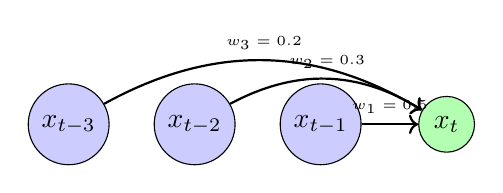
\begin{tikzpicture}[scale=0.8]
\node[circle,draw,fill=blue!20] (x1) at (0,0) {$x_{t-3}$};
\node[circle,draw,fill=blue!20] (x2) at (2,0) {$x_{t-2}$};
\node[circle,draw,fill=blue!20] (x3) at (4,0) {$x_{t-1}$};
\node[circle,draw,fill=green!30] (xt) at (6,0) {$x_t$};

\draw[->,thick] (x1) to[bend left] node[above,font=\tiny] {$w_3=0.2$} (xt);
\draw[->,thick] (x2) to[bend left] node[above,font=\tiny] {$w_2=0.3$} (xt);
\draw[->,thick] (x3) -- node[above,font=\tiny] {$w_1=0.5$} (xt);
\end{tikzpicture}
\end{center}


\paragraph{自回归模型的问题}
\begin{theorem}[问题1:窗口大小 $\tau$ 如何选择?]
\begin{itemize}
    \item $\tau$ 太小:丢失长期信息,如季节性规律
    \item $\tau$ 太大:参数太多,计算复杂,过拟合
\end{itemize}
\end{theorem}




\begin{definition}[理想情况]
我们希望:\textbf{参数数量固定},但能\textbf{记住所有历史}!
\end{definition}


\paragraph{隐变量自回归模型}
\textbf{关键思想:}引入一个\textbf{隐变量}(hidden state)$h_t$ 来总结历史

\begin{definition}[数学形式]
\begin{align*}
h_t &= g(h_{t-1}, x_{t-1}) \quad \text{\textcolor{blue}{(更新记忆)}}\\
x_t &= f(h_t) + \epsilon_t \quad \text{\textcolor{red}{(生成预测)}}
\end{align*}
\end{definition}

\textbf{直观理解:}
\begin{itemize}
    \item $h_t$:像大脑的\textbf{记忆},存储到时刻 $t$ 的所有重要信息
    \item $g$:\textbf{更新函数},根据新观测 $x_{t-1}$ 更新记忆
    \item $f$:\textbf{输出函数},根据当前记忆预测未来
\end{itemize}

\begin{center}
\begin{tikzpicture}[scale=1.1]
\node[circle,draw,fill=red!20,minimum size=1cm] (h1) at (0,1.5) {$h_1$};
\node[circle,draw,fill=red!20,minimum size=1cm] (h2) at (2,1.5) {$h_2$};
\node[circle,draw,fill=red!20,minimum size=1cm] (h3) at (4,1.5) {$h_3$};
\node[circle,draw,fill=red!20,minimum size=1cm] (h4) at (6,1.5) {$h_4$};

\node[circle,draw,fill=blue!20] (x1) at (0,0) {$x_1$};
\node[circle,draw,fill=blue!20] (x2) at (2,0) {$x_2$};
\node[circle,draw,fill=blue!20] (x3) at (4,0) {$x_3$};
\node[circle,draw,fill=green!30] (x4) at (6,0) {$x_4$};

\draw[->,thick] (x1) -- (h1);
\draw[->,thick] (x2) -- (h2);
\draw[->,thick] (x3) -- (h3);
\draw[->,thick] (h1) -- (h2) node[midway,above,font=\tiny] {$g$};
\draw[->,thick] (h2) -- (h3) node[midway,above,font=\tiny] {$g$};
\draw[->,thick] (h3) -- (h4) node[midway,above,font=\tiny] {$g$};
\draw[->,thick] (h4) -- (x4) node[midway,right,font=\tiny] {$f$};

\node[below,font=\small] at (3,-0.7) {隐状态像"记忆",不断更新};
\end{tikzpicture}
\end{center}


\paragraph{隐变量模型的优势}


\textbf{标准自回归:}
\begin{center}
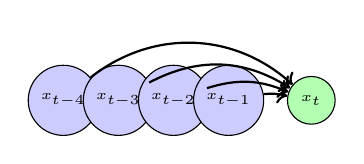
\begin{tikzpicture}[scale=0.7]
\node[circle,draw,fill=blue!20,font=\tiny] (x1) at (0,0) {$x_{t-4}$};
\node[circle,draw,fill=blue!20,font=\tiny] (x2) at (1,0) {$x_{t-3}$};
\node[circle,draw,fill=blue!20,font=\tiny] (x3) at (2,0) {$x_{t-2}$};
\node[circle,draw,fill=blue!20,font=\tiny] (x4) at (3,0) {$x_{t-1}$};
\node[circle,draw,fill=green!30,font=\tiny] (xt) at (4.5,0) {$x_t$};

\draw[->,thick] (x1) to[bend left=40] (xt);
\draw[->,thick] (x2) to[bend left=30] (xt);
\draw[->,thick] (x3) to[bend left=20] (xt);
\draw[->,thick] (x4) to[bend left=10] (xt);
\end{tikzpicture}
\end{center}

\textcolor{red}{\textbf{问题:}}
\begin{itemize}
    \item 输入维度 = $\tau$
    \item 历史越长,输入越大
    \item 参数数量:$\tau \times d$
\end{itemize}


\textbf{隐变量模型:}
\begin{center}
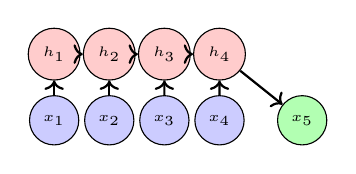
\begin{tikzpicture}[scale=0.7]
\node[circle,draw,fill=red!20,font=\tiny] (h1) at (0,1.2) {$h_1$};
\node[circle,draw,fill=red!20,font=\tiny] (h2) at (1,1.2) {$h_2$};
\node[circle,draw,fill=red!20,font=\tiny] (h3) at (2,1.2) {$h_3$};
\node[circle,draw,fill=red!20,font=\tiny] (h4) at (3,1.2) {$h_4$};

\node[circle,draw,fill=blue!20,font=\tiny] (x1) at (0,0) {$x_1$};
\node[circle,draw,fill=blue!20,font=\tiny] (x2) at (1,0) {$x_2$};
\node[circle,draw,fill=blue!20,font=\tiny] (x3) at (2,0) {$x_3$};
\node[circle,draw,fill=blue!20,font=\tiny] (x4) at (3,0) {$x_4$};
\node[circle,draw,fill=green!30,font=\tiny] (x5) at (4.5,0) {$x_5$};

\foreach \i in {1,2,3,4} {
    \draw[->,thick] (x\i) -- (h\i);
}
\draw[->,thick] (h1) -- (h2);
\draw[->,thick] (h2) -- (h3);
\draw[->,thick] (h3) -- (h4);
\draw[->,thick] (h4) -- (x5);
\end{tikzpicture}
\end{center}

\textcolor{blue}{\textbf{优势:}}
\begin{itemize}
    \item 输入维度固定
    \item 无论历史多长
    \item 参数数量不变
\end{itemize}


\vspace{0.5cm}
\begin{theorem}[关键创新]
$h_t$ 就像一个\textbf{压缩包},把所有历史信息压缩存储!\\
这就是\textbf{循环神经网络(RNN)}的核心思想!
\end{theorem}


\paragraph{隐状态的直观类比}
\begin{center}
\begin{tikzpicture}[scale=1.1]
% 人脑
%\node[inner sep=0] at (0,2) {\includegraphics[width=1.5cm]{brain.png}};
\node[below,text width=3cm,align=center] at (0,0.8) {
\textbf{人类记忆}\\
看到新信息\\
$\downarrow$\\
更新记忆\\
$\downarrow$\\
基于记忆决策
};

% 箭头
\draw[->,ultra thick] (1.5,2) -- (3.5,2);

% 隐状态
\node[circle,draw,fill=red!30,minimum size=1.5cm] at (5,2) {$h_t$};
\node[below,text width=3cm,align=center] at (5,0.8) {
\textbf{隐状态}\\
观测到 $x_{t-1}$\\
$\downarrow$\\
更新 $h_t = g(h_{t-1}, x_{t-1})$\\
$\downarrow$\\
预测 $x_t = f(h_t)$
};

% 箭头
\draw[->,ultra thick] (6.5,2) -- (8.5,2);

% RNN
%\node[inner sep=0] at (10,2) {\includegraphics[width=1.5cm]{rnn.png}};
\node[below,text width=3cm,align=center] at (10,0.8) {
\textbf{循环神经网络}\\
实现隐状态\\
的具体架构
};

\end{tikzpicture}
\end{center}

\begin{definition}[类比]
隐状态 $h_t$ = 你看完前面所有剧集后的记忆\\
你不记得每一个细节,但记得关键信息!
\end{definition}



\subsection{训练}

\section{8.1.2 训练}

\paragraph{ 训练序列模型}
\begin{center}
\Large \textcolor{blue}{有了模型,如何从数据中学习参数?}
\end{center}


\paragraph{训练的基本思路}
\textbf{给定:}训练序列 $x_1, x_2, x_3, \ldots, x_T$

\textbf{目标:}找到最优参数,使模型预测尽可能准确

\begin{definition}[训练三步骤]
\begin{enumerate}
    \item \textbf{定义模型}:选择 $f$ 和 $g$ 的具体形式
    \item \textbf{定义损失函数}:衡量预测与真实值的差距
    \item \textbf{优化参数}:用梯度下降最小化损失
\end{enumerate}
\end{definition}

\begin{center}
\begin{tikzpicture}[scale=1.0]
\node[draw,fill=yellow!20,rounded corners,text width=2.5cm,align=center] at (0,0) {
训练数据\\
$\{x_1, \ldots, x_T\}$
};

\draw[->,thick] (1.5,0) -- (2.5,0);

\node[draw,fill=blue!20,rounded corners,text width=2cm,align=center] at (4,0) {
模型\\
$x_t = f_\theta(x_{<t})$
};

\draw[->,thick] (5.5,0) -- (6.5,0);

\node[draw,fill=red!20,rounded corners,text width=2cm,align=center] at (8,0) {
损失函数\\
$L(\theta)$
};

\draw[->,thick] (8,-0.8) -- (4,-0.8);
\node[below,font=\small] at (6,-1) {梯度下降优化};
\end{tikzpicture}
\end{center}


\paragraph{例子:训练线性自回归模型}
\textbf{模型:}$x_t = w_1 x_{t-1} + w_2 x_{t-2} + b$

\textbf{损失:}均方误差 $L = \frac{1}{T}\sum_{t=1}^{T}(x_t - \hat{x}_t)^2$

% \begin{lstlisting}
% import torch
% import torch.nn as nn
% 
% # Generate simulated data( + )
% T = 1000
% time = torch.arange(1, T + 1, dtype=torch.float32)
% x = torch.sin(0.01 * time) + torch.randn(T) * 0.2
% 
% # Prepare training datausing2time steppredictionnext step
% tau = 2
% features = torch.zeros((T - tau, tau))
% for i in range(tau):
%     features[:, i] = x[i: T - tau + i]
% labels = x[tau:].reshape((-1, 1))
% 
% # Define linear model
% model = nn.Linear(tau, 1)
% loss_fn = nn.MSELoss()
% optimizer = torch.optim.SGD(model.parameters(), lr=0.01)
% \end{lstlisting}


\paragraph{训练循环}
\begin{lstlisting}
# training
num_epochs = 10
for epoch in range(num_epochs):
    predictions = model(features)
    loss = loss_fn(predictions, labels)
    
    optimizer.zero_grad()
    loss.backward()
    optimizer.step()
    
    if (epoch + 1) % 2 == 0:
        print(f'Epoch {epoch+1}, Loss: {loss.item():.4f}')

# Output
# Epoch 2, Loss: 0.0523
# Epoch 4, Loss: 0.0418
# Epoch 6, Loss: 0.0387
# Epoch 8, Loss: 0.0372
# Epoch 10, Loss: 0.0365
\end{lstlisting}

\begin{definition}[训练过程]
损失逐渐下降 $\to$ 模型学到了数据的规律
\end{definition}


\section{8.1.3 预测}

\subsection{8.1.3 预测}
\begin{center}
\Large \textcolor{blue}{训练完模型后,如何用它来预测?}
\end{center}


\paragraph{单步预测 vs 多步预测}


\textbf{单步预测(One-step Ahead):}
\begin{center}
\begin{tikzpicture}[scale=0.8]
\foreach \i in {1,...,5} {
    \node[circle,draw,fill=blue!20,font=\tiny] (x\i) at (\i*0.8,0) {$x_{\i}$};
}
\node[circle,draw,fill=green!30,font=\tiny] (x6) at (5.6,0) {$\hat{x}_6$};

\draw[->,thick,red] (x5) -- (x6);
\draw[decorate,decoration={brace,amplitude=5pt},thick] (0.4,-0.5) -- (4.4,-0.5);
\node[below] at (2.4,-0.7) {\tiny 已知};
\node[below,green!60!black] at (5.6,-0.5) {\tiny 预测};
\end{tikzpicture}
\end{center}

\textbf{特点:}
\begin{itemize}
    \item 只预测\textbf{下一步}
    \item 使用\textbf{真实}历史数据
    \item 准确度高
\end{itemize}


\textbf{多步预测(Multi-step Ahead):}
\begin{center}
\begin{tikzpicture}[scale=0.8]
\foreach \i in {1,2,3} {
    \node[circle,draw,fill=blue!20,font=\tiny] (x\i) at (\i*0.8,0) {$x_{\i}$};
}
\foreach \i in {4,5,6} {
    \node[circle,draw,fill=green!30,font=\tiny] (x\i) at (\i*0.8,0) {$\hat{x}_{\i}$};
}

\draw[->,thick,red] (x3) -- (x4);
\draw[->,thick,red] (x4) -- (x5);
\draw[->,thick,red] (x5) -- (x6);
\draw[decorate,decoration={brace,amplitude=5pt},thick] (0.4,-0.5) -- (2.6,-0.5);
\node[below] at (1.5,-0.7) {\tiny 已知};
\node[below,green!60!black] at (4.4,-0.5) {\tiny 多步预测};
\end{tikzpicture}
\end{center}

\textbf{特点:}
\begin{itemize}
    \item 预测\textbf{未来多步}
    \item 使用\textbf{预测值}作输入
    \item 误差会累积
\end{itemize}


\vspace{0.5cm}
\begin{theorem}[核心区别]
单步预测:$\hat{x}_{t+1} = f(x_t, x_{t-1}, \ldots)$ $\leftarrow$ 用真实值\\
多步预测:$\hat{x}_{t+k} = f(\hat{x}_{t+k-1}, \hat{x}_{t+k-2}, \ldots)$ $\leftarrow$ 用预测值
\end{theorem}


\paragraph{多步预测的误差累积}
\begin{center}
\begin{tikzpicture}[scale=1.1]
% 时间轴
\draw[->,thick] (0,0) -- (9,0) node[right] {时间步};
\draw[->,thick] (0,0) -- (0,3.5) node[above] {值};

% 真实值(蓝色实线)
\draw[blue,thick] (1,1.5) -- (2,1.8) -- (3,2.0) -- (4,1.9) -- (5,2.1) -- (6,2.3) -- (7,2.2) -- (8,2.4);
\foreach \x/\y in {1/1.5, 2/1.8, 3/2.0, 4/1.9, 5/2.1, 6/2.3, 7/2.2, 8/2.4} {
    \fill[blue] (\x,\y) circle (2pt);
}

% 预测值(红色虚线,误差越来越大)
\draw[red,thick,dashed] (3,2.0) -- (4,1.85) -- (5,1.95) -- (6,1.9) -- (7,1.7) -- (8,1.5);
\foreach \x/\y in {4/1.85, 5/1.95, 6/1.9, 7/1.7, 8/1.5} {
    \fill[red] (\x,\y) circle (2pt);
}

% 标注
\draw[blue,thick] (0.5,3.2) -- (1.5,3.2) node[right,black] {真实值};
\draw[red,thick,dashed] (0.5,2.8) -- (1.5,2.8) node[right,black] {预测值};

% 误差标注
\draw[<->,thick,purple] (6,2.3) -- (6,1.9) node[midway,right] {\tiny 误差};
\draw[<->,thick,purple] (8,2.4) -- (8,1.5) node[midway,right] {\tiny 累积误差};

% 分界线
\draw[thick,green!60!black,dashed] (3,-0.3) -- (3,3);
\node[below,green!60!black] at (3,-0.3) {预测起点};
\end{tikzpicture}
\end{center}

\begin{theorem}[误差累积现象]
\begin{itemize}
    \item 第1步预测有小误差 $\epsilon_1$
    \item 第2步基于有误差的预测,误差变大 $\epsilon_1 + \epsilon_2$
    \item 第3步误差继续累积...
    \item 预测越远,误差越大!
\end{itemize}
\end{theorem}


\paragraph{单步预测代码示例}
\begin{lstlisting}
# Single-step prediction using real historical data
def predict_one_step(model, x_history, tau):
    """ x_history: shape (tau,) Return: next step prediction """
    with torch.no_grad():
        x_input = x_history[-tau:].reshape(1, -1)
        prediction = model(x_input)
    return prediction.item()

x_true = torch.tensor([1.0, 1.2, 1.1, 1.3, 1.2])
next_value = predict_one_step(model, x_true, tau=2)
print(f"Based on {x_true[-2:].tolist()} predict: {next_value:.3f}")

# Output
# Based on [1.3, 1.2] predict: 1.245
\end{lstlisting}

\begin{definition}[关键]
使用\textbf{真实的}历史数据 $x_{t-1}, x_{t-2}, \ldots$ 作为输入
\end{definition}


\paragraph{多步预测:递归策略}
\begin{lstlisting}
# Multi-step prediction using recursive strategy
def predict_multi_step(model, x_history, tau, k_steps):
    """ x_history: initial history data, shape (tau,) k_steps: number of steps to predict Return: k prediction values """
    predictions = []
    current_input = x_history[-tau:].clone()
    
    for _ in range(k_steps):
        # Predict next step
        with torch.no_grad():
            next_pred = model(current_input.reshape(1, -1))
        predictions.append(next_pred.item())
        
        # Update input with prediction
        current_input = torch.cat([current_input[1:], 
                                   next_pred.reshape(1)])
    
    return predictions

predictions = predict_multi_step(model, x_true, tau=2, k_steps=5)
print(f"Future 5-step predictions: {predictions}")
# Output: Future 5-step predictions: [1.245, 1.233, 1.239, 1.236, 1.237]
\end{lstlisting}


\paragraph{多步预测的可视化}
\begin{center}
\begin{tikzpicture}[scale=1.0]
% 标题
\node[font=\large\bfseries] at (5,4) {递归多步预测过程};

% 步骤1
\node[draw,fill=blue!20,text width=8cm] at (5,3) {
\textbf{步骤1:} 用真实历史 $[x_3, x_4]$ $\to$ 预测 $\hat{x}_5$
};

% 步骤2
\node[draw,fill=yellow!20,text width=8cm] at (5,2) {
\textbf{步骤2:} 用 $[x_4, \hat{x}_5]$ $\to$ 预测 $\hat{x}_6$
};

% 步骤3
\node[draw,fill=orange!20,text width=8cm] at (5,1) {
\textbf{步骤3:} 用 $[\hat{x}_5, \hat{x}_6]$ $\to$ 预测 $\hat{x}_7$
};

% 步骤4
\node[draw,fill=red!20,text width=8cm] at (5,0) {
\textbf{步骤4:} 用 $[\hat{x}_6, \hat{x}_7]$ $\to$ 预测 $\hat{x}_8$
};

% 箭头
\foreach \y in {2.5,1.5,0.5} {
    \draw[->,ultra thick] (5,\y+0.3) -- (5,\y-0.3);
}

\end{tikzpicture}
\end{center}

\begin{theorem}[注意]
从步骤2开始,输入中就包含了\textbf{预测值},不再是真实值!
\end{theorem}


\paragraph{多步预测的两种策略对比}


\textbf{策略1:递归预测}\\
(Autoregressive/Recursive)

\begin{center}
\begin{tikzpicture}[scale=0.7]
\node[draw,circle,fill=blue!20] (m) at (2,1.5) {模型};
\node[left] at (0,1.5) {$x_{t-1}, x_t$};
\node[right] at (4,1.5) {$\hat{x}_{t+1}$};
\draw[->,thick] (0.8,1.5) -- (m);
\draw[->,thick] (m) -- (3.2,1.5);
\draw[->,thick,red] (3.2,1.5) to[bend right=40] (0.8,0.5);
\node[below] at (2,0.3) {反馈到输入};
\end{tikzpicture}
\end{center}

\textcolor{blue}{\textbf{优点:}}
\begin{itemize}
    \item 只需1个模型
    \item 灵活,可预测任意步数
\end{itemize}

\textcolor{red}{\textbf{缺点:}}
\begin{itemize}
    \item 误差累积
    \item 长期预测不准
\end{itemize}


\textbf{策略2:直接预测}\\
(Direct/MIMO)

\begin{center}
\begin{tikzpicture}[scale=0.7]
\node[draw,circle,fill=green!20,font=\tiny] (m1) at (1,2) {模型1};
\node[draw,circle,fill=green!20,font=\tiny] (m2) at (1,1) {模型2};
\node[draw,circle,fill=green!20,font=\tiny] (m3) at (1,0) {模型k};

\node[left,font=\tiny] at (-0.5,1) {$x_{t-1}, x_t$};
\foreach \i in {1,2,3} {
    \draw[->,thick] (-0.3,1) -- (m\i);
}

\node[right,font=\tiny] at (3,2) {$\hat{x}_{t+1}$};
\node[right,font=\tiny] at (3,1) {$\hat{x}_{t+2}$};
\node[right,font=\tiny] at (3,0) {$\hat{x}_{t+k}$};

\draw[->,thick] (m1) -- (2.3,2);
\draw[->,thick] (m2) -- (2.3,1);
\draw[->,thick] (m3) -- (2.3,0);
\end{tikzpicture}
\end{center}

\textcolor{blue}{\textbf{优点:}}
\begin{itemize}
    \item 无误差累积
    \item 每步独立优化
\end{itemize}

\textcolor{red}{\textbf{缺点:}}
\begin{itemize}
    \item 需要训练k个模型
    \item 计算开销大
\end{itemize}



\paragraph{预测horizon的选择}
\textbf{问题:}应该预测多远的未来?

\begin{center}
\begin{tikzpicture}[scale=1.0]
% 坐标轴
\draw[->,thick] (0,0) -- (8,0) node[right] {预测步数 $k$};
\draw[->,thick] (0,0) -- (0,3) node[above] {误差};

% 误差曲线
\draw[blue,thick,domain=0:7,samples=50] plot (\x,{0.5+0.3*\x+0.05*\x*\x});

% 标注
\node[blue,above] at (2,1.2) {误差随步数增长};
\fill[red] (3,2.1) circle (3pt);
\node[red,above] at (3,2.3) {可接受的horizon};

% 阴影区
\fill[green!20,opacity=0.3] (0,0) rectangle (3,3);
\node[green!60!black] at (1.5,2.5) {可用区};

\fill[red!20,opacity=0.3] (3,0) rectangle (8,3);
\node[red!60!black] at (5.5,2.5) {误差太大};

\end{tikzpicture}
\end{center}

\begin{definition}[经验法则]
\begin{itemize}
    \item 短期预测(1-10步):通常可靠
    \item 中期预测(10-100步):取决于数据规律性
    \item 长期预测($>$100步):非常困难,需要强正则化
\end{itemize}
\end{definition}


\paragraph{实战:预测效果对比}


\begin{lstlisting}[basicstyle=\ttfamily\tiny]
# sequence
x_true = [1.0, 1.2, 1.1, 
          1.3, 1.2, 1.4,
          1.3, 1.5, 1.4]

# Single-step predictionusing real
single_step = []
for i in range(3, 9):
    pred = model(x_true[i-2:i])
    single_step.append(pred)

# [1.25, 1.20, 1.35, ...]
\end{lstlisting}


\begin{lstlisting}[basicstyle=\ttfamily\tiny]
# multi-steppredictionprediction
multi_step = []
input = x_true[1:3]  # [1.2, 1.1]
for _ in range(6):
    pred = model(input)
    multi_step.append(pred)
    input = [input[1], pred]

# [1.25, 1.18, 1.27, ...]
\end{lstlisting}


\vspace{0.5cm}
\begin{center}
\begin{tabular}{|c|c|c|c|}
\hline
\textbf{时间步} & \textbf{真实值} & \textbf{单步预测} & \textbf{多步预测} \\
\hline
4 & 1.3 & 1.25 & 1.25 \\
5 & 1.2 & 1.20 & 1.18 \\
6 & 1.4 & 1.35 & 1.27 \\
7 & 1.3 & 1.32 & 1.22 \\
\hline
\end{tabular}
\end{center}

\begin{theorem}[观察]
多步预测的误差明显大于单步预测!
\end{theorem}


\paragraph{预测的实际应用}
\begin{definition}[不同场景的预测需求]
\begin{itemize}
    \item \textbf{天气预报}:需要未来3-7天预测(多步)
    \item \textbf{股票交易}:高频交易只关心下一刻(单步)
    \item \textbf{语言模型}:生成文本需要长序列预测(多步)
    \item \textbf{异常检测}:只需要预测下一个值并比较(单步)
\end{itemize}
\end{definition}

\begin{theorem}[关键权衡]
\begin{itemize}
    \item 单步预测:准确但只能看"一步之遥"
    \item 多步预测:能看"更远"但不够准确
    \item 实际应用需要根据任务选择合适的策略
\end{itemize}
\end{theorem}


\section{8.2 文本预处理}

\paragraph{进入 8.2 文本预处理}
\begin{center}
\Large \textcolor{blue}{从数值序列到文本序列}
\end{center}

\vspace{0.5cm}
\begin{definition}[之前学的(8.1节)]
\begin{itemize}
    \item 处理数值序列(股价、温度等)
    \item 输入和输出都是\textbf{连续值}
\end{itemize}
\end{definition}

\begin{definition}[现在要学的(8.2节)]
\begin{itemize}
    \item 处理文本序列(句子、文章等)
    \item 输入和输出是\textbf{离散符号}(词、字符)
    \item 需要特殊的预处理步骤
\end{itemize}
\end{definition}

\begin{theorem}[核心问题]
如何把文本转换成数字,让神经网络能处理?
\end{theorem}


\subsection{8.2 文本预处理 - 章节导航}
\begin{definition}[本节内容]
\begin{itemize}
    \item 8.2.1 读取数据集
    \item 8.2.2 词元化 (Tokenization)
    \item 8.2.3 词表 (Vocabulary)
    \item 8.2.4 整合所有功能
\end{itemize}
\end{definition}

\begin{theorem}[学习目标]
\begin{enumerate}
    \item 学会读取和清洗文本
    \item 理解不同的词元化策略
    \item 掌握构建词表的方法
    \item 能将文本转为数字序列
\end{enumerate}
\end{theorem}





\section{未命名节}

\subsection{读取数据集}

\subsection{8.2.1 读取数据集}

\subsection{8.2.1 读取数据集}
\begin{center}
\Large \textcolor{blue}{第一步:获取原始文本}
\end{center}


\paragraph{为什么需要文本预处理?}
\begin{center}
\begin{tikzpicture}
\node[text width=8cm,draw,fill=yellow!20,rounded corners] at (0,3) {
\textbf{原始文本:}\\
``The Time Machine, by H.G. Wells [1898]''\\
``It was at ten o'clock to-day that...''
};

\draw[->,ultra thick] (0,2.2) -- (0,1.5);
\node at (2,1.8) {需要转换};

\node[text width=8cm,draw,fill=green!20,rounded corners] at (0,0.5) {
\textbf{数字序列:}\\
234, 567, 123, 89, 456, ...\\
计算机才能处理!
};
\end{tikzpicture}
\end{center}

\begin{definition}[文本预处理的挑战]
\begin{itemize}
    \item 文本是\textbf{离散}的符号
    \item 包含大小写、标点、特殊字符
    \item 需要统一的处理流程
\end{itemize}
\end{definition}


\paragraph{时光机器数据集}
\textbf{数据集:}H.G. Wells的科幻小说《时光机器》(The Time Machine, 1895)

\begin{example}[为什么选这个数据集?]
\begin{itemize}
    \item 英文文本,便于处理
    \item 大小适中(约30KB,3万多词)
    \item 语言规范,句子结构清晰
    \item 开源免费
\end{itemize}
\end{example}

\begin{center}
\begin{tikzpicture}
\node[draw,fill=yellow!20,rounded corners,text width=8cm,align=left,font=\small] at (5,0) {
\textbf{原始文本片段:}\\
\textit{``The Time Machine, by H. G. Wells [1898]''}\\
\textit{``I''}\\
\textit{``The Time Traveller (for so it will be convenient to speak of him)''}\\
\textit{``was expounding a recondite matter to us...''}
};
\end{tikzpicture}
\end{center}

\begin{theorem}[特点]
包含标题、章节标记、对话、描述等多种文本形式
\end{theorem}


\paragraph{读取文本文件}
\begin{lstlisting}
import os
import requests

# data
def download_data():
    url = 'http://d2l-data.s3-accelerate.amazonaws.com/timemachine.txt'
    response = requests.get(url)
    with open('timemachine.txt', 'wb') as f:
        f.write(response.content)

def read_time_machine():
    with open('timemachine.txt', 'r', encoding='utf-8') as f:
        lines = f.readlines()
    return lines

lines = read_time_machine()
print(f"Total lines: {len(lines)}")
print(f"First 3 lines:")
for i in range(3):
    print(f"Line {i}: {lines[i]}")
\end{lstlisting}

\textbf{输出:}
\begin{verbatim}
Total lines: 3221
Line 0: The Time Machine, by H. G. Wells [1898]
Line 1: 
Line 2: I
\end{verbatim}


\paragraph{原始文本的"脏数据"}
\textbf{问题:}原始文本包含很多"噪声"



\textbf{常见噪声:}
\begin{itemize}
    \item 大小写混杂\\
    \texttt{"The", "the", "THE"}
    \item 标点符号\\
    \texttt{"Hello!", "Hello?", "Hello."}
    \item 特殊字符\\
    \texttt{"don't", "it's", "---"}
    \item 空行和空格
    \item 数字\\
    \texttt{"year 1898"}
\end{itemize}


\begin{theorem}[为什么要清洗?]
\begin{itemize}
    \item 减少词汇量
    \item 统一表示形式
    \item 避免稀疏性问题
    \item 提高模型泛化能力
\end{itemize}
\end{theorem}

\begin{example}[例子]
不清洗:\\
"The", "the", "THE" $\to$ 3个词

清洗后:\\
"the" $\to$ 1个词
\end{example}



\paragraph{文本清洗}
\begin{lstlisting}
import re

def read_time_machine():
    with open('timemachine.txt', 'r') as f:
        lines = f.readlines()
    
    clean_lines = []
    for line in lines:
        # 1. 
        line = line.lower()
        # 2. 
        line = re.sub('[^a-z]+', ' ', line)
        # 3. 
        line = line.strip()
        # 4. 
        if line:
            clean_lines.append(line)
    
    return clean_lines

lines_raw = read_raw()
lines_clean = read_time_machine()
print("Raw:", lines_raw[0])
print("Clean:", lines_clean[0])
\end{lstlisting}

\textbf{输出:}
\begin{verbatim}
Raw: The Time Machine, by H. G. Wells [1898]
Clean: the time machine by h g wells
\end{verbatim}


\paragraph{正则表达式快速入门}
\textbf{正则表达式(Regex):}强大的文本匹配工具

\begin{center}
\begin{tabular}{|l|l|l|}
\hline
\textbf{模式} & \textbf{含义} & \textbf{示例} \\
\hline
\texttt{[a-z]} & 匹配小写字母 & \texttt{"a", "b", "z"} \\
\texttt{[A-Z]} & 匹配大写字母 & \texttt{"A", "B", "Z"} \\
\texttt{[0-9]} & 匹配数字 & \texttt{"0", "5", "9"} \\
\texttt{[a-zA-Z]} & 匹配所有字母 & \texttt{"a", "B", "z"} \\
\texttt{\^{}} & 取反 & \texttt{[\^{}a-z]} = 非小写字母 \\
\texttt{+} & 一个或多个 & \texttt{[a-z]+} = 多个字母 \\
\hline
\end{tabular}
\end{center}

\begin{example}[应用示例]
\begin{itemize}
    \item 
    把所有\textbf{非小写字母}替换为空格
    
    \item 
    把所有\textbf{数字}替换为特殊标记
\end{itemize}
\end{example}


\paragraph{清洗前后对比}


\textbf{清洗前:}
\begin{lstlisting}[basicstyle=\ttfamily\tiny]
The Time Machine, 
by H. G. Wells [1898]

I

The Time Traveller 
(for so it will be 
convenient to speak of him)
was expounding a 
recondite matter to us.
\end{lstlisting}


\textbf{清洗后:}
\begin{lstlisting}[basicstyle=\ttfamily\tiny]
the time machine by h g wells

i

the time traveller for so 
it will be convenient to 
speak of him was expounding 
a recondite matter to us
\end{lstlisting}


\vspace{0.5cm}
\begin{definition}[观察]
\begin{itemize}
    \item 全部小写
    \item 标点消失
    \item 数字消失
    \item 保留了空格(词与词之间的分隔)
\end{itemize}
\end{definition}

\subsection{8.2.2 词元化}

\subsection{8.2.2 词元化(Tokenization)}
\begin{center}
\Large \textcolor{blue}{把文本拆分成"词元"(token)}
\end{center}


\paragraph{什么是词元?}
\textbf{词元(Token):}文本的基本处理单位

\begin{center}
\begin{tikzpicture}[scale=1.1]
% 原始句子
\node[text width=10cm,align=center,font=\large] at (5,3.5) {
\textbf{原始句子:}"the time traveller was smiling"
};

\draw[->,ultra thick] (5,3) -- (5,2.5);

% 词元化
\node[draw,fill=blue!20,rounded corners] at (1,2) {the};
\node[draw,fill=blue!20,rounded corners] at (2.5,2) {time};
\node[draw,fill=blue!20,rounded corners] at (4.2,2) {traveller};
\node[draw,fill=blue!20,rounded corners] at (6,2) {was};
\node[draw,fill=blue!20,rounded corners] at (7.5,2) {smiling};

\node[below,font=\small] at (4.5,1.3) {5个词元(tokens)};

\end{tikzpicture}
\end{center}

\begin{theorem}[为什么需要词元化?]
\begin{itemize}
    \item 神经网络只能处理\textbf{固定大小}的输入
    \item 需要将连续的文本拆分成\textbf{离散单元}
    \item 词元是\textbf{特征提取}的基础
\end{itemize}
\end{theorem}


\paragraph{词元化的三种粒度}
\begin{center}
\begin{tikzpicture}[scale=1.0]
% 原始句子
\node[font=\large] at (6,4.5) {\textbf{句子:}"natural language processing"};

% 词级别
\node[draw,fill=green!20,text width=10cm,align=left] at (6,3.2) {
\textbf{1. 词级别(Word-level)}\\
\texttt{["natural", "language", "processing"]} \\
$\to$ 3个词元
};

% 字符级别
\node[draw,fill=yellow!20,text width=10cm,align=left] at (6,1.8) {
\textbf{2. 字符级别(Character-level)}\\
\texttt{["n","a","t","u","r","a","l"," ","l","a","n","g",...]} \\
$\to$ 27个词元
};

% 子词级别
\node[draw,fill=orange!20,text width=10cm,align=left] at (6,0.4) {
\textbf{3. 子词级别(Subword-level)}\\
\texttt{["natur", "al", "language", "process", "ing"]} \\
$\to$ 5个词元
};

\end{tikzpicture}
\end{center}


\paragraph{词级别词元化}
\textbf{策略:}按空格或标点分割



\textcolor{blue}{\textbf{优点:}}
\begin{itemize}
    \item \checkmark 语义清晰
    \item \checkmark 符合人类理解
    \item \checkmark 适合大多数任务
\end{itemize}

\textcolor{red}{\textbf{缺点:}}
\begin{itemize}
    \item $\times$ 词表很大
    \item $\times$ 未登录词(OOV)问题
    \item $\times$ 形态变化(如:run/running)
\end{itemize}


\begin{example}[OOV问题]
\textbf{训练集:}\\
\texttt{"dog", "cat", "run"}

\textbf{测试时遇到:}\\
\texttt{"dogs", "running", "bird"}

$\rightarrow$ 模型不认识!
\end{example}


\vspace{0.3cm}
\begin{definition}[词表大小]
英文:常用词汇 5万-10万\\
中文:常用汉字 3千-5千,但词汇量更大
\end{definition}


\paragraph{词级别词元化代码}
\begin{lstlisting}
def tokenize_word_level(text):
    """Simple function"""
    return text.split()

text = "the time traveller was smiling"
tokens = tokenize_word_level(text)
print(f"tokens: {tokens}")
print(f"tokens数: {len(tokens)}")

# Output
# tokens: ['the', 'time', 'traveller', 'was', 'smiling']
# tokens: 5

# data
lines = read_time_machine()
all_tokens = []
for line in lines:
    all_tokens.extend(tokenize_word_level(line))

print(f"总tokens数: {len(all_tokens)}")
print(f"前20个tokens: {all_tokens[:20]}")
\end{lstlisting}

\textbf{输出:}
\begin{lstlisting}[language=Python]
总tokens数: 32775
前20个tokens: ['the', 'time', 'machine', 'by', 'h', 'g', ...]
\end{lstlisting}


\paragraph{字符级别词元化}
\textbf{策略:}把每个字符作为一个词元



\textcolor{blue}{\textbf{优点:}}
\begin{itemize}
    \item \checkmark 词表极小(26个字母)
    \item \checkmark 无OOV问题
    \item \checkmark 能处理任意文本
    \item \checkmark 对拼写错误鲁棒
\end{itemize}

\textcolor{red}{\textbf{缺点:}}
\begin{itemize}
    \item $\times$ 序列变得很长
    \item $\times$ 训练慢
    \item $\times$ 难以捕捉词级别语义
\end{itemize}


\begin{example}[例子]
\textbf{输入:}\\
\texttt{"cat"}

\textbf{词级别:}\\
1个词元:\texttt{["cat"]}

\textbf{字符级别:}\\
3个词元:\texttt{["c","a","t"]}
\end{example}

\begin{theorem}[序列长度]
"hello world" (11个字符)\\
vs \\
"hello world" (2个单词)\\
序列长度差5倍!
\end{theorem}



\paragraph{字符级别词元化代码}
\begin{lstlisting}
def tokenize_char_level(text):
    """tokens"""
    return list(text)

text = "the time"
tokens = tokenize_char_level(text)
print(f"tokens: {tokens}")
print(f"tokens数: {len(tokens)}")

# Output
# tokens: ['t', 'h', 'e', ' ', 't', 'i', 'm', 'e']
# tokens: 8

# Calculate vocabulary size
lines = read_time_machine()
text = ' '.join(lines)
chars = set(text)
print(f"字符集大小: {len(chars)}")
print(f"字符集: {sorted(chars)}")
\end{lstlisting}

\textbf{输出:}
\begin{verbatim}
字符集大小: 27
字符集: [' ', 'a', 'b', 'c', ..., 'z']
\end{verbatim}

\begin{definition}[观察]
词表从5万缩小到27个!但序列长度增加5-10倍
\end{definition}


\paragraph{子词级别词元化}
\textbf{核心思想:}介于词和字符之间的折中方案

\begin{center}
\begin{tikzpicture}[scale=1.0]
% 示意图
\node[font=\large] at (5,3.5) {\textbf{例子:}``unhappiness''};

\draw[->,thick] (5,3.2) -- (5,2.7);

% 词级别
\node[draw,fill=red!20] at (2,2) {``unhappiness''};
\node[below,font=\tiny,text width=3cm,align=center] at (2,1.5) {词级别:1个词元\\但可能OOV};

% 子词级别
\node[draw,fill=green!20] at (5,2) {``un'' + ``happi'' + ``ness''};
\node[below,font=\tiny,text width=3cm,align=center] at (5,1.5) {子词级别:3个词元\\可组合成新词};

% 字符级别
\node[draw,fill=yellow!20,font=\small] at (8,2) {``u'',``n'',``h'',``a'',...};
\node[below,font=\tiny,text width=3cm,align=center] at (8,1.5) {字符级别:11个词元\\序列太长};

\end{tikzpicture}
\end{center}

\begin{definition}[子词的好处]
\begin{itemize}
    \item 可以组合出训练集中没见过的词
    \item 例如:"unhappy" = "un" + "happy"
    \item 即使没见过"unhappy",也能理解它的意思
\end{itemize}
\end{definition}


\paragraph{常见子词算法}
\begin{enumerate}
\item \textbf{BPE (Byte Pair Encoding)}
\begin{itemize}
    \item 从字符开始,迭代合并最频繁的相邻pair
    \item GPT-2, RoBERTa使用
\end{itemize}

\item \textbf{WordPiece}
\begin{itemize}
    \item 类似BPE,但用likelihood而非频率
    \item BERT使用
\end{itemize}

\item \textbf{SentencePiece}
\begin{itemize}
    \item 直接从原始文本训练,不依赖预分词
    \item 支持多语言
    \item T5, XLNet使用
\end{itemize}
\end{enumerate}

\begin{theorem}[现代NLP趋势]
大模型几乎都使用\textbf{子词级别}词元化!\\
平衡了词表大小和序列长度
\end{theorem}


\paragraph{三种粒度对比总结}
\begin{center}
\begin{tabular}{|l|c|c|c|}
\hline
\textbf{特性} & \textbf{词级别} & \textbf{字符级别} & \textbf{子词级别} \\
\hline
词表大小 & 很大(5万+) & 很小($\sim$100) & 中等(3万) \\
\hline
序列长度 & 短 & 很长 & 中等 \\
\hline
OOV问题 & 严重 & 无 & 轻微 \\
\hline
语义保留 & 好 & 差 & 较好 \\
\hline
训练速度 & 快 & 慢 & 中等 \\
\hline
应用场景 & 传统NLP & 生成任务 & 现代大模型 \\
\hline
\end{tabular}
\end{center}

\vspace{0.5cm}
\begin{definition}[本节使用]
为了简单起见,我们使用\textbf{词级别}词元化\\
在8.4节实现RNN时,会用\textbf{字符级别}
\end{definition}


\paragraph{完整词元化函数}
\begin{lstlisting}
def tokenize(lines, token_type='word'):
    """ tokens lines: token_type: 'word' 'char' Return: tokens """
    if token_type == 'word':
        return [line.split() for line in lines]
    elif token_type == 'char':
        return [list(line) for line in lines]
    else:
        raise ValueError(f"Unknown token_type: {token_type}")

lines = read_time_machine()
tokens_word = tokenize(lines, 'word')
tokens_char = tokenize(lines, 'char')

print(f"词级别 - 第1行: {tokens_word[0]}")
print(f"字符级别 - 第1行: {tokens_char[0]}")
\end{lstlisting}

\textbf{输出:}
\begin{verbatim}
词级别 - 第1行: ['the', 'time', 'machine', 'by', 'h', 'g', 'wells']
字符级别 - 第1行: ['t','h','e',' ','t','i','m','e',...]
\end{verbatim}



\subsection{词表}

\subsection{8.2.3 词表}

\subsection{8.2.3 词表(Vocabulary)}
\begin{center}
\Large \textcolor{blue}{建立词元到数字的映射}
\end{center}


\paragraph{为什么需要词表?}
\textbf{问题:}神经网络不能直接处理文本

\begin{center}
\begin{tikzpicture}[scale=1.1]
% 文本
\node[draw,fill=yellow!20,rounded corners,text width=3cm,align=center] at (0,2) {
文本\\
"cat"
};

\draw[->,ultra thick,red] (1.5,2) -- (2.5,2);
\node[red,above] at (2,2.2) {\text{×}不能直接用};

% 神经网络
\node[draw,fill=blue!20,rounded corners,text width=3cm,align=center] at (4.5,2) {
神经网络\\
需要数字
};

% 解决方案
\draw[->,ultra thick,green!60!black] (0,1.2) -- (0,0.5);
\node[draw,fill=green!20,rounded corners,text width=3cm,align=center] at (0,0) {
数字\\
词表["cat"]=42
};

\draw[->,ultra thick,green!60!black] (1.5,0) -- (2.5,2);
\node[green!60!black,below] at (2,1) {$\checkmark$通过词表转换};

\end{tikzpicture}
\end{center}

\begin{theorem}[词表的作用]
建立\textbf{词元 $\leftrightarrow$ 数字}的双向映射
\end{theorem}


\paragraph{词表构建示例}
\textbf{输入文本:}"the cat sat on the mat"

\begin{center}
\begin{tikzpicture}[scale=1.0]
% 步骤1:词元化
\node[draw,fill=yellow!20,text width=8cm] at (5,3.5) {
\textbf{步骤1:词元化}\\
\texttt{["the", "cat", "sat", "on", "the", "mat"]}
};

\draw[->,thick] (5,3) -- (5,2.5);

% 步骤2:统计频率
\node[draw,fill=orange!20,text width=8cm] at (5,2) {
\textbf{步骤2:统计词频}\\
\texttt{"the": 2, "cat": 1, "sat": 1, "on": 1, "mat": 1}
};

\draw[->,thick] (5,1.5) -- (5,1);

% 步骤3:按频率排序+分配ID
\node[draw,fill=green!20,text width=8cm,align=left] at (5,0.2) {
\textbf{步骤3:构建词表(按频率排序)}\\
\texttt{0: <unk>  (未知词)}\\
\texttt{1: the    (freq=2)}\\
\texttt{2: cat    (freq=1)}\\
\texttt{3: mat    (freq=1)}\\
\texttt{4: on     (freq=1)}\\
\texttt{5: sat    (freq=1)}
};

\end{tikzpicture}
\end{center}


\paragraph{特殊词元}
\textbf{除了普通词,词表还包含特殊标记:}

\begin{center}
\begin{tabular}{|l|l|l|}
\hline
\textbf{符号} & \textbf{含义} & \textbf{用途} \\
\hline
\texttt{<unk>} & Unknown & 未知词,词表中没有的词 \\
\hline
\texttt{<pad>} & Padding & 填充,对齐不同长度序列 \\
\hline
\texttt{<bos>} & Begin of Sequence & 句子开始标记 \\
\hline
\texttt{<eos>} & End of Sequence & 句子结束标记 \\
\hline
\texttt{<mask>} & Mask & 掩码,用于BERT等模型 \\
\hline
\end{tabular}
\end{center}

\begin{example}[例子]
\textbf{原始:}"hello world"

\textbf{加特殊标记:}\\
\texttt{[<bos>, "hello", "world", <eos>]}

\textbf{转数字(假设词表):}\\
\texttt{[1, 234, 567, 2]}
\end{example}


\paragraph{词频统计}
\begin{lstlisting}
def count_corpus(tokens):
    """tokens"""
    # tokens1D2D
    if len(tokens) == 0 or isinstance(tokens[0], list):
        # 2D1D
        tokens = [token for line in tokens for token in line]
    
    from collections import Counter
    return Counter(tokens)

lines = read_time_machine()
tokens = tokenize(lines, 'word')
counter = count_corpus(tokens)

print(f"总tokens数: {sum(counter.values())}")
print(f"不同tokens数: {len(counter)}")
print(f"最常见的10个词: {counter.most_common(10)}")
\end{lstlisting}

\textbf{输出:}
\begin{verbatim}
总词元数: 32775
不同词元数: 4580
最常见的10个词: [('the', 2261), ('i', 1267), ('and', 1245), ...]
\end{verbatim}


\paragraph{词表类实现 - 初始化}
\begin{lstlisting}
class Vocab:
    def __init__(self, tokens=None, min_freq=0, 
                 reserved_tokens=None):
        """ tokens: tokens min_freq: reserved_tokens: tokens(<pad>) """
        if tokens is None:
            tokens = []
        if reserved_tokens is None:
            reserved_tokens = []
        
        counter = count_corpus(tokens)
        self._token_freqs = sorted(counter.items(), 
                                   key=lambda x: x[1], 
                                   reverse=True)
        
        # tokens0tokens1
        self.idx_to_token = ['<unk>'] + reserved_tokens
        self.token_to_idx = {token: idx 
                for idx, token in enumerate(self.idx_to_token)}
\end{lstlisting}


\paragraph{词表类实现 - 构建映射}
\begin{lstlisting}
        for token, freq in self._token_freqs:
            if freq < min_freq:
                break
            if token not in self.token_to_idx:
                self.idx_to_token.append(token)
                self.token_to_idx[token] = len(self.idx_to_token) - 1
    
    def __len__(self):
        """vocabulary"""
        return len(self.idx_to_token)
    
    def __getitem__(self, tokens):
        """查询tokens对应的索引"""
        if not isinstance(tokens, (list, tuple)):
            return self.token_to_idx.get(tokens, self.unk)
        return [self.__getitem__(token) for token in tokens]
    
    @property
    def unk(self):
        """未知词的索引,总是0"""
        return 0
    
    def to_tokens(self, indices):
        """索引转回tokens"""
        if not isinstance(indices, (list, tuple)):
            return self.idx_to_token[indices]
        return [self.idx_to_token[index] for index in indices]
\end{lstlisting}


\paragraph{词表使用示例}
\begin{lstlisting}
# vocabulary
lines = read_time_machine()
tokens = tokenize(lines, 'word')
vocab = Vocab(tokens)

print(f"vocabulary大小: {len(vocab)}")
print(f"前10个tokens: {vocab.idx_to_token[:10]}")

# tokens
test_tokens = ['the', 'time', 'machine', 'xyz']
indices = vocab[test_tokens]
print(f"tokens: {test_tokens}")
print(f"索引: {indices}")

# tokens
back_tokens = vocab.to_tokens(indices)
print(f"转回: {back_tokens}")
\end{lstlisting}

\textbf{输出:}
\begin{verbatim}
词表大小: 4581
前10个词元: ['<unk>', 'the', 'i', 'and', 'of', 'a', ...]
词元: ['the', 'time', 'machine', 'xyz']
索引: [1, 19, 50, 0]
转回: ['the', 'time', 'machine', '<unk>']
\end{verbatim}

\begin{theorem}[注意]
'xyz'不在词表中,被映射到 \texttt{<unk>} (索引0)
\end{theorem}


\paragraph{最小频率阈值的作用}
\textbf{问题:}低频词很多,但作用不大

\begin{center}
\begin{tikzpicture}[scale=1.0]
% Zipf定律图示
\draw[->,thick] (0,0) -- (8,0) node[right] {词频排名};
\draw[->,thick] (0,0) -- (0,4) node[above] {词频};

% 曲线
\draw[blue,thick,domain=0.5:7.5,samples=100] plot (\x,{3.5/\x});

% 高频区
\fill[green!20,opacity=0.5] (0,0) rectangle (2,4);
\node[green!60!black] at (1,3.5) {\tiny 高频词};
\node[green!60!black,below] at (1,0) {\tiny 保留};

% 中频区
\fill[yellow!20,opacity=0.5] (2,0) rectangle (5,4);
\node[orange!60!black] at (3.5,2) {\tiny 中频词};

% 低频区
\fill[red!20,opacity=0.5] (5,0) rectangle (8,4);
\node[red!60!black] at (6.5,1) {\tiny 低频词};
\node[red!60!black,below] at (6.5,0) {\tiny 丢弃};

% 阈值线
\draw[red,dashed,thick] (0,0.7) -- (8,0.7);
\node[red,left] at (0,0.7) {\tiny min\_freq};

\end{tikzpicture}
\end{center}

\begin{definition}[策略]
\begin{itemize}
    \item \texttt{min\_freq=0}:保留所有词(词表大)
    \item \texttt{min\_freq=5}:至少出现5次才保留(减小词表)
    \item 低频词通常是拼写错误、人名等,可以用 \texttt{<unk>} 代替
\end{itemize}
\end{definition}


\paragraph{最小频率阈值示例}
\begin{lstlisting}
vocab_all = Vocab(tokens, min_freq=0)
vocab_5 = Vocab(tokens, min_freq=5)
vocab_10 = Vocab(tokens, min_freq=10)

print(f"min_freq=0:  vocabulary大小={len(vocab_all)}")
print(f"min_freq=5:  vocabulary大小={len(vocab_5)}")
print(f"min_freq=10: vocabulary大小={len(vocab_10)}")

counter = count_corpus(tokens)
low_freq = [token for token, freq in counter.items() if freq < 5]
print(f"频率<5的词数: {len(low_freq)}")
print(f"示例: {low_freq[:10]}")
\end{lstlisting}

\textbf{输出:}
\begin{verbatim}
min_freq=0:  词表大小=4581
min_freq=5:  词表大小=2034
min_freq=10: 词表大小=1446
频率<5的词数: 3143
示例: ['1898', 'xiv', 'pg', 'redistribution', ...]
\end{verbatim}

\begin{theorem}[观察]
68\%的词频率$<$5,但它们只占总词数的很小比例!
\end{theorem}



\subsection{整合所有功能}

\subsection{8.2.4 整合所有功能}

\subsection{8.2.4 整合所有功能}
\begin{center}
\Large \textcolor{blue}{完整的文本预处理流程}
\end{center}


\paragraph{完整流程总结}
\begin{center}
\begin{tikzpicture}[scale=0.95]
% 步骤1
\node[draw,fill=yellow!20,rounded corners,text width=10cm] at (5,4.5) {
\textbf{步骤1: 读取数据}\\
\texttt{lines = read\_time\_machine()}
};

\draw[->,thick] (5,4) -- (5,3.5);

% 步骤2
\node[draw,fill=orange!20,rounded corners,text width=10cm] at (5,3) {
\textbf{步骤2: 词元化}\\
\texttt{tokens = tokenize(lines, 'word')}
};

\draw[->,thick] (5,2.5) -- (5,2);

% 步骤3
\node[draw,fill=green!20,rounded corners,text width=10cm] at (5,1.5) {
\textbf{步骤3: 构建词表}\\
\texttt{vocab = Vocab(tokens, min\_freq=5)}
};

\draw[->,thick] (5,1) -- (5,0.5);

% 步骤4
\node[draw,fill=blue!20,rounded corners,text width=10cm] at (5,0) {
\textbf{步骤4: 转换为索引}\\
\texttt{corpus = [vocab[token] for line in tokens for token in line]}
};

\end{tikzpicture}
\end{center}


\paragraph{一站式函数}
\begin{lstlisting}
def load_corpus_time_machine(max_tokens=-1):
    """ Returndatatokensvocabulary max_tokens: tokens,-1 """
    lines = read_time_machine()
    # tokens
    tokens = tokenize(lines, 'char')  # comment
    # vocabulary
    vocab = Vocab(tokens)
    corpus = [vocab[token] for line in tokens for token in line]
    if max_tokens > 0:
        corpus = corpus[:max_tokens]
    
    return corpus, vocab

corpus, vocab = load_corpus_time_machine()
print(f"语料库length: {len(corpus)}")
print(f"vocabulary大小: {len(vocab)}")
print(f"前10个索引: {corpus[:10]}")
print(f"对应tokens: {vocab.to_tokens(corpus[:10])}")
\end{lstlisting}


\paragraph{一站式函数输出}
\begin{lstlisting}[basicstyle=\ttfamily\tiny]
# Output
语料库length: 170580
vocabulary大小: 28
前10个索引: [1, 8, 5, 0, 1, 9, 13, 5, 0, 13]
对应tokens: ['t', 'h', 'e', ' ', 't', 'i', 'm', 'e', ' ', 'm']
\end{lstlisting}

\begin{definition}[观察]
\begin{itemize}
    \item 使用\textbf{字符级别}词元化
    \item 语料库是一个很长的数字序列(17万+)
    \item 词表只有28个字符(26个字母+空格+其他)
    \item 每个索引对应词表中的一个字符
\end{itemize}
\end{definition}

\begin{theorem}[为什么用字符级别?]
\begin{itemize}
    \item RNN训练时序列不宜过长
    \item 字符级别词表小,便于演示
    \item 避免OOV问题
\end{itemize}
\end{theorem}


\paragraph{文本$\to$数字的完整示例}
\begin{center}
\begin{tikzpicture}[scale=1.0]
% 原始文本
\node[draw,fill=yellow!20,rounded corners,text width=10cm,align=center] at (5,4) {
\textbf{原始文本}\\
``the time machine''
};

\draw[->,thick] (5,3.5) -- (5,3.2);
\node[right] at (5.5,3.35) {\tiny 清洗};

% 清洗后
\node[draw,fill=orange!20,rounded corners,text width=10cm,align=center] at (5,2.8) {
\textbf{清洗后}\\
``the time machine''
};

\draw[->,thick] (5,2.4) -- (5,2.1);
\node[right] at (5.5,2.25) {\tiny 词元化(字符级)};

% 词元
\node[draw,fill=green!20,rounded corners,text width=10cm,align=center] at (5,1.7) {
\textbf{词元列表}\\
t, h, e, (space), t, i, m, e, (space), m, a, c, h, i, n, e
};

\draw[->,thick] (5,1.3) -- (5,1.0);
\node[right] at (5.5,1.15) {\tiny 词表映射};

% 索引
\node[draw,fill=blue!20,rounded corners,text width=10cm,align=center] at (5,0.6) {
\textbf{索引序列}\\
20, 8, 5, 0, 20, 9, 13, 5, 0, 13, 1, 3, 8, 9, 14, 5
};

\draw[->,thick] (5,0.2) -- (5,-0.1);

% 神经网络
\node[draw,fill=red!20,rounded corners,text width=10cm,align=center] at (5,-0.5) {
\textbf{输入神经网络} \checkmark
};

\end{tikzpicture}
\end{center}


\paragraph{词表可视化}
\begin{center}
\begin{tikzpicture}[scale=1.0]
% 标题
\node[font=\large\bfseries] at (5,4) {词表结构(字符级别)};

% 词表
\node[draw,fill=yellow!20,text width=10cm,align=left,font=\small] at (5,2) {
\textbf{词表(部分):}\\
\texttt{0: ' '  (空格)}\\
\texttt{1: 'a'}\\
\texttt{2: 'b'}\\
\texttt{3: 'c'}\\
\texttt{4: 'd'}\\
\texttt{5: 'e'}\\
\texttt{...}\\
\texttt{20: 't'}\\
\texttt{...}\\
\texttt{26: 'z'}
};

% 双向映射
\node[draw,fill=green!20,text width=4cm,align=center] at (1,0) {
字符 $\to$ 索引\\
\texttt{'t' $\to$ 20}
};

\draw[<->,ultra thick] (3.5,0) -- (6.5,0);

\node[draw,fill=blue!20,text width=4cm,align=center] at (9,0) {
索引 $\to$ 字符\\
\texttt{20 $\to$ 't'}
};

\end{tikzpicture}
\end{center}


\paragraph{完整数据加载器(带批处理)}
\begin{lstlisting}
def load_data_time_machine(batch_size, num_steps, 
                           use_random_iter=False):
    """ Returndataiterationvocabulary batch_size: num_steps: time step use_random_iter: """
    corpus, vocab = load_corpus_time_machine()
    
    # dataiteration8.3
    if use_random_iter:
        data_iter = seq_data_iter_random(corpus, batch_size, num_steps)
    else:
        data_iter = seq_data_iter_sequential(corpus, batch_size, num_steps)
    
    return data_iter, vocab

batch_size, num_steps = 32, 35
train_iter, vocab = load_data_time_machine(batch_size, num_steps)
\end{lstlisting}


\subsection{8.2节总结}
\begin{definition}[核心流程]
\begin{enumerate}
    \item \textbf{读取数据}:从文件读取原始文本
    \item \textbf{清洗}:转小写、去标点、去数字
    \item \textbf{词元化}:拆分成词元(词/字符/子词)
    \item \textbf{构建词表}:统计词频,建立索引映射
    \item \textbf{数值化}:将文本转为数字序列
\end{enumerate}
\end{definition}

\begin{theorem}[关键概念]
\begin{itemize}
    \item \textbf{词元(Token)}:文本的基本单位
    \item \textbf{词表(Vocabulary)}:词元$\leftrightarrow$索引的映射
    \item \textbf{语料库(Corpus)}:数值化后的文本序列
    \item \textbf{特殊标记}:\texttt{<unk>}, \texttt{<pad>}, \texttt{<bos>}, \texttt{<eos>}
\end{itemize}
\end{theorem}


\paragraph{三种词元化策略对比}
\begin{center}
\begin{tikzpicture}[scale=0.9]
% 表格形式
\node[font=\small] at (5,4) {\textbf{句子:"I love natural language processing"}};

% 词级别
\node[draw,fill=green!20,text width=10cm,align=left] at (5,3) {
\textbf{词级别:}\\
5个词元: \texttt{["I", "love", "natural", "language", "processing"]}\\
词表大: 需要5万+ | 有OOV问题
};

% 子词级别
\node[draw,fill=yellow!20,text width=10cm,align=left] at (5,1.8) {
\textbf{子词级别:}\\
7个词元: \texttt{["I", "love", "natur", "al", "language", "process", "ing"]}\\
词表中: 需要3万左右 | 几乎无OOV
};

% 字符级别
\node[draw,fill=orange!20,text width=10cm,align=left] at (5,0.6) {
\textbf{字符级别:}\\
33个词元: \texttt{["I", " ", "l", "o", "v", "e", " ", "n", ...]}\\
词表小: 只需100左右 | 序列太长
};

\end{tikzpicture}
\end{center}

\begin{definition}[选择建议]
\begin{itemize}
    \item 教学/演示 $\to$ 字符级别(简单)
    \item 传统任务 $\to$ 词级别(快速)
    \item 现代大模型 $\to$ 子词级别(平衡)
\end{itemize}
\end{definition}


\paragraph{实战tips}


\textbf{常见问题:}
\begin{enumerate}
    \item \textbf{词表太大}\\
    $\to$ 提高 \texttt{min\_freq}\\
    $\to$ 使用子词

    \item \textbf{OOV太多}\\
    $\to$ 降低 \texttt{min\_freq}\\
    $\to$ 使用字符/子词
    
    \item \textbf{序列太长}\\
    $\to$ 使用词级别\\
    $\to$ 截断序列
\end{enumerate}


\textbf{优化建议:}
\begin{enumerate}
    \item 根据任务选择粒度
    \item 合理设置频率阈值
    \item 考虑特殊标记需求
    \item 保存词表以便复用
    \item 可视化词频分布
\end{enumerate}


\vspace{0.5cm}
\begin{theorem}[下一步]
有了数值化的文本,接下来学习如何构建\textbf{语言模型}(8.3节)
\end{theorem}


\subsection{8.2节关键代码总结}
\begin{center}
\begin{tikzpicture}[scale=0.9]
% 核心函数
\node[draw,fill=yellow!20,text width=10cm,align=left,font=\small] at (5,3.5) {
\textbf{核心函数:}\\
\texttt{read\_time\_machine()} - 读取并清洗文本\\
\texttt{tokenize(lines, type)} - 词元化\\
\texttt{count\_corpus(tokens)} - 统计词频\\
\texttt{Vocab(tokens, min\_freq)} - 构建词表\\
\texttt{load\_corpus\_time\_machine()} - 一站式加载
};

% Vocab类关键方法
\node[draw,fill=green!20,text width=10cm,align=left,font=\small] at (5,1.5) {
\textbf{Vocab类关键方法:}\\
\texttt{vocab[token]} - 词元$\to$索引\\
\texttt{vocab.to\_tokens(idx)} - 索引$\to$词元\\
\texttt{len(vocab)} - 词表大小\\
\texttt{vocab.unk} - 未知词索引(=0)
};

% 数据流
\node[draw,fill=blue!20,text width=10cm,align=center,font=\small] at (5,0) {
\textbf{数据流:}\\
文本 $\to$ 清洗 $\to$ 词元 $\to$ 词表 $\to$ 索引 $\to$ 神经网络
};

\end{tikzpicture}
\end{center}

\section{8.3 语言模型和数据集}

\subsection{8.3 语言模型和数据集 - 章节导航}
\begin{definition}[本节内容]
\begin{itemize}
    \item 8.3.1 学习语言模型
    \item 8.3.2 马尔可夫模型与元语法
    \item 8.3.3 自然语言统计
    \item 8.3.4 读取长序列数据
\end{itemize}
\end{definition}

\begin{theorem}[学习目标]
\begin{enumerate}
    \item 理解语言模型的数学定义
    \item 掌握困惑度(Perplexity)的计算
    \item 了解马尔可夫假设
    \item 学会构建序列数据迭代器
\end{enumerate}
\end{theorem}





\section{未命名节}

\subsection{学习语言模型}

\subsection{8.3.1 学习语言模型}

\subsection{8.3.1 学习语言模型}
\begin{center}
\Large \textcolor{blue}{语言模型的核心:估计文本序列的概率}
\end{center}


\paragraph{什么是语言模型?}
\textbf{定义:}语言模型对文本序列的概率分布进行建模

\begin{definition}[数学表示]
对于文本序列 $x_1, x_2, \ldots, x_T$,语言模型估计其概率:
$$P(x_1, x_2, \ldots, x_T)$$
\end{definition}

\textbf{链式法则分解:}
$$P(x_1, x_2, \ldots, x_T) = \prod_{t=1}^{T} P(x_t \mid x_1, \ldots, x_{t-1})$$

\begin{example}[直观理解]
给定前面的词,预测下一个词的概率
\begin{itemize}
    \item 已知:``the cat sat on the''
    \item 预测:下一个词是 ``mat'' 的概率?
\end{itemize}
\end{example}


\paragraph{语言模型的应用}


\textbf{1. 文本生成}
\begin{itemize}
    \item 对话系统
    \item 故事创作
    \item 代码补全
\end{itemize}

\textbf{2. 机器翻译}
\begin{itemize}
    \item 评估译文流畅度
    \item 选择最佳翻译
\end{itemize}


\textbf{3. 语音识别}
\begin{itemize}
    \item 纠正识别错误
    \item 消除歧义
\end{itemize}

\textbf{4. 拼写检查}
\begin{itemize}
    \item 检测错误
    \item 提供建议
\end{itemize}


\vspace{0.5cm}
\begin{theorem}[核心思想]
好的语言模型能给\textbf{合理的句子}分配\textbf{高概率},给\textbf{不合理的句子}分配\textbf{低概率}
\end{theorem}


\paragraph{语言模型的挑战}
\textbf{问题:}直接估计 $P(x_1, x_2, \ldots, x_T)$ 非常困难!

\begin{center}
\begin{tikzpicture}[scale=1.0]
% 序列长度
\node[draw,fill=yellow!20,text width=10cm] at (5,3.5) {
\textbf{挑战1:序列长度不固定}\\
不同句子长度不同,如何统一建模?
};

% 参数数量
\node[draw,fill=orange!20,text width=10cm] at (5,2.2) {
\textbf{挑战2:参数爆炸}\\
如果词表大小为 $V$,长度为 $T$ 的序列有 $V^T$ 种可能!
};

% 稀疏性
\node[draw,fill=red!20,text width=10cm] at (5,0.9) {
\textbf{挑战3:数据稀疏}\\
很多序列在训练集中从未出现,如何估计概率?
};

\end{tikzpicture}
\end{center}

\begin{definition}[解决思路]
\begin{itemize}
    \item 使用\textbf{链式法则}分解
    \item 使用\textbf{马尔可夫假设}简化
    \item 使用\textbf{神经网络}建模条件概率
\end{itemize}
\end{definition}


\paragraph{条件概率建模}
\textbf{关键:}将复杂的联合概率分解为条件概率的乘积

$$P(x_1, x_2, x_3, x_4) = P(x_1) \cdot P(x_2 \mid x_1) \cdot P(x_3 \mid x_1, x_2) \cdot P(x_4 \mid x_1, x_2, x_3)$$

\begin{center}
\begin{tikzpicture}[scale=1.1]
% 时间步
\foreach \i in {1,2,3,4} {
    \node[circle,draw,fill=blue!20] (x\i) at (\i*2,0) {$x_{\i}$};
}

% 条件依赖
\draw[->,thick,red] (x1) to[bend left=30] node[above,font=\tiny] {$P(x_2|x_1)$} (x2);
\draw[->,thick,red] (x1) to[bend left=40] (x3);
\draw[->,thick,red] (x2) to[bend left=30] node[above,font=\tiny] {$P(x_3|x_1,x_2)$} (x3);
\draw[->,thick,red] (x1) to[bend left=50] (x4);
\draw[->,thick,red] (x2) to[bend left=40] (x4);
\draw[->,thick,red] (x3) to[bend left=30] node[above,font=\tiny] {$P(x_4|x_1,x_2,x_3)$} (x4);

\node[below,font=\small] at (4,-0.7) {每个词依赖前面所有词};
\end{tikzpicture}
\end{center}

\begin{theorem}[关键问题]
如何高效地估计条件概率 $P(x_t \mid x_1, \ldots, x_{t-1})$?
\end{theorem}


\paragraph{困惑度(Perplexity)}
\textbf{定义:}评估语言模型质量的标准指标

\begin{definition}[数学定义]
$$\text{PPL} = \exp\left(-\frac{1}{n}\sum_{t=1}^{n}\log P(x_t \mid x_1, \ldots, x_{t-1})\right)$$
\end{definition}

\textbf{等价形式:}
$$\text{PPL} = \sqrt[n]{\frac{1}{P(x_1, x_2, \ldots, x_n)}}$$



\textbf{直观理解:}
\begin{itemize}
    \item 平均分支因子
    \item 模型的``困惑程度''
    \item 越低越好
\end{itemize}


\textbf{取值范围:}
\begin{itemize}
    \item 最好:PPL = 1(完全确定)
    \item 随机猜测:PPL = $|V|$
    \item 实际:10-200之间
\end{itemize}



\paragraph{困惑度的直观例子}
\textbf{例子:}预测下一个词

\begin{center}
\begin{tikzpicture}[scale=1.0]
% 好的模型
\node[draw,fill=green!20,text width=5cm] at (0,3) {
\textbf{模型A(好):}\\
``I love''后面是:\\
- ``you'': 0.7\\
- ``it'': 0.2\\
- ``apple'': 0.1\\
\textbf{PPL} $\approx$ \textbf{2.1}
};

% 差的模型
\node[draw,fill=red!20,text width=5cm] at (0,0.5) {
\textbf{模型B(差):}\\
``I love''后面是:\\
- ``you'': 0.01\\
- ``it'': 0.01\\
- 其他998个词均分\\
\textbf{PPL} $\approx$ \textbf{100}
};

% 标注
\node[right,text width=4cm] at (6,3) {
\textcolor{green!60!black}{$\checkmark$ 集中在合理的词上}\\
困惑度低
};

\node[right,text width=4cm] at (6,0.5) {
\textcolor{red}{$\times$ 概率分散}\\
困惑度高
};

\end{tikzpicture}
\end{center}


\paragraph{困惑度计算示例}
\begin{lstlisting}
import torch
import torch.nn.functional as F

def calculate_perplexity(model, data, vocab):
    """model"""
    model.eval()
    total_loss = 0
    total_tokens = 0
    
    with torch.no_grad():
        for X, Y in data:
            # X: (batch_size, seq_len)
            # Y: (batch_size, seq_len)
            output = model(X)  # (batch_size, seq_len, vocab_size)
            
            # loss
            loss = F.cross_entropy(
                output.reshape(-1, len(vocab)),
                Y.reshape(-1),
                reduction='sum'
            )
            
            total_loss += loss.item()
            total_tokens += Y.numel()
    
    #  = exp()
    perplexity = torch.exp(torch.tensor(total_loss / total_tokens))
    return perplexity.item()
\end{lstlisting}



\subsection{马尔可夫模型与元语法}

\subsection{8.3.2 马尔可夫模型与元语法}

\subsection{8.3.2 马尔可夫模型与元语法}
\begin{center}
\Large \textcolor{blue}{简化建模:马尔可夫假设}
\end{center}


\paragraph{马尔可夫假设}
\textbf{问题:}依赖所有历史太复杂

$$P(x_t \mid x_1, x_2, \ldots, x_{t-1})$$

\textbf{马尔可夫假设:}只依赖最近的 $\tau$ 个词

$$P(x_t \mid x_1, x_2, \ldots, x_{t-1}) \approx P(x_t \mid x_{t-\tau}, \ldots, x_{t-1})$$

\begin{center}
\begin{tikzpicture}[scale=1.0]
% 完整依赖
\node[text width=10cm] at (5,3.5) {
\textbf{完整模型:}依赖所有历史
};
\foreach \i in {1,2,3,4,5} {
    \node[circle,draw,fill=blue!20,font=\tiny] (x\i) at (\i*1.5,2.5) {$x_{\i}$};
}
\node[circle,draw,fill=green!30] (x6) at (10,2.5) {$x_6$};
\foreach \i in {1,2,3,4,5} {
    \draw[->,thick,red] (x\i) to[bend left=20] (x6);
}

% 马尔可夫
\node[text width=10cm] at (5,1.2) {
\textbf{马尔可夫模型:}只依赖最近 $\tau=2$ 个
};
\foreach \i in {1,2,3,4,5} {
    \node[circle,draw,fill=blue!20,font=\tiny] (y\i) at (\i*1.5,0) {$x_{\i}$};
}
\node[circle,draw,fill=green!30] (y6) at (10,0) {$x_6$};
\draw[->,thick,red] (y4) to[bend left=20] (y6);
\draw[->,thick,red] (y5) to[bend left=20] (y6);
\end{tikzpicture}
\end{center}


\paragraph{N-gram模型}
\textbf{根据 $\tau$ 的不同,有不同的N-gram模型:}

\begin{center}
\begin{tabular}{|l|l|l|}
\hline
\textbf{模型} & \textbf{$\tau$} & \textbf{条件概率} \\
\hline
Unigram (1-gram) & 0 & $P(x_t)$ \\
\hline
Bigram (2-gram) & 1 & $P(x_t \mid x_{t-1})$ \\
\hline
Trigram (3-gram) & 2 & $P(x_t \mid x_{t-2}, x_{t-1})$ \\
\hline
4-gram & 3 & $P(x_t \mid x_{t-3}, x_{t-2}, x_{t-1})$ \\
\hline
\end{tabular}
\end{center}

\begin{example}[例子:Bigram模型]
\textbf{句子:}``the cat sat on the mat''

\textbf{概率:}
\begin{align*}
P(\text{sentence}) &= P(\text{the}) \cdot P(\text{cat} \mid \text{the}) \cdot P(\text{sat} \mid \text{cat}) \\
&\quad \cdot P(\text{on} \mid \text{sat}) \cdot P(\text{the} \mid \text{on}) \cdot P(\text{mat} \mid \text{the})
\end{align*}
\end{example}


\paragraph{N-gram模型的估计}
\textbf{最大似然估计(MLE):}

$$P(x_t \mid x_{t-\tau}, \ldots, x_{t-1}) = \frac{\text{count}(x_{t-\tau}, \ldots, x_{t-1}, x_t)}{\text{count}(x_{t-\tau}, \ldots, x_{t-1})}$$

\begin{example}[Bigram例子]
训练文本:``I love you I love coding I love AI''

\textbf{计算:}$P(\text{you} \mid \text{love})$

$$P(\text{you} \mid \text{love}) = \frac{\text{count}(\text{love you})}{\text{count}(\text{love})} = \frac{1}{3}$$

其他:
\begin{itemize}
    \item $P(\text{coding} \mid \text{love}) = 1/3$
    \item $P(\text{AI} \mid \text{love}) = 1/3$
\end{itemize}
\end{example}


\paragraph{N-gram模型的问题}


\textbf{优点:}
\begin{itemize}
    \item $\checkmark$ 简单高效
    \item $\checkmark$ 易于实现
    \item $\checkmark$ 可解释性强
\end{itemize}


\textbf{缺点:}
\begin{itemize}
    \item $\times$ 无法捕捉长期依赖
    \item $\times$ 数据稀疏问题严重
    \item $\times$ 参数随 $\tau$ 指数增长
\end{itemize}


\vspace{0.5cm}
\begin{theorem}[数据稀疏问题]
\textbf{例子:}训练集中没见过 ``love machine''

$\Rightarrow$ $P(\text{machine} \mid \text{love}) = 0$

\textbf{解决:}平滑技术(Laplace平滑、Good-Turing平滑等)
\end{theorem}

\begin{definition}[现代方案]
使用\textbf{神经网络语言模型}(如RNN)克服这些问题
\end{definition}


\paragraph{N-gram模型实现}
\begin{lstlisting}
from collections import defaultdict, Counter

class NgramModel:
    def __init__(self, n=2):
        self.n = n
        self.context_counts = defaultdict(Counter)
    
    def train(self, corpus):
        """trainingN-grammodel"""
        for i in range(self.n - 1, len(corpus)):
            context = tuple(corpus[i - self.n + 1:i])
            word = corpus[i]
            self.context_counts[context][word] += 1
    
    def prob(self, context, word):
        """计算条件概率 P(word | context)"""
        context = tuple(context)
        if context not in self.context_counts:
            return 0
        
        total = sum(self.context_counts[context].values())
        return self.context_counts[context][word] / total
\end{lstlisting}



\subsection{自然语言统计}

\subsection{8.3.3 自然语言统计}

\subsection{8.3.3 自然语言统计}
\begin{center}
\Large \textcolor{blue}{真实文本的统计规律}
\end{center}


\paragraph{Zipf定律}
\textbf{定律:}词频与其排名成反比

$$\text{frequency}(k) \propto \frac{1}{k^\alpha}$$

其中 $k$ 是词频排名,$\alpha \approx 1$

\begin{center}
\begin{tikzpicture}[scale=1.0]
% 坐标轴
\draw[->,thick] (0,0) -- (8,0) node[right] {词频排名(对数尺度)};
\draw[->,thick] (0,0) -- (0,4) node[above] {词频(对数尺度)};

% Zipf曲线
\draw[blue,thick,domain=0.5:7.5,samples=100] plot (\x,{3.5-0.5*\x});

% 标注
\node[blue] at (2,3) {the};
\node[blue] at (3,2.3) {of};
\node[blue] at (4,1.8) {and};
\node[blue] at (6,1) {machine};

% 直线拟合
\draw[red,dashed,thick] (0.5,3.2) -- (7.5,0.2);
\node[red,right] at (7.5,0.2) {$y = -\alpha x + c$};

\node[below,text width=8cm,align=center] at (4,-0.8) {
\small 少数高频词 + 大量低频词
};
\end{tikzpicture}
\end{center}


\paragraph{Zipf定律的含义}


\textbf{长尾分布:}
\begin{itemize}
    \item 少数词非常常见
    \item 大部分词很少见
    \item ``the'', ``of'', ``and'' 占比很大
\end{itemize}

\textbf{影响:}
\begin{itemize}
    \item 词表大小选择
    \item 低频词处理
    \item 采样策略
\end{itemize}


\begin{example}[时光机器数据]
\begin{itemize}
    \item 总词数:32,775
    \item 不同词数:4,580
    \item Top 10占比:30\%
    \item Top 100占比:50\%
    \item 出现1次的词:50\%
\end{itemize}
\end{example}


\vspace{0.3cm}
\begin{theorem}[启示]
可以用 \texttt{min\_freq} 过滤低频词,减小词表但保留大部分信息
\end{theorem}


\paragraph{可视化Zipf定律}
\begin{lstlisting}
import matplotlib.pyplot as plt
import numpy as np

counter = count_corpus(tokens)
freqs = sorted(counter.values(), reverse=True)

plt.figure(figsize=(10, 5))

plt.subplot(1, 2, 1)
plt.loglog(range(1, len(freqs) + 1), freqs)
plt.xlabel('Rank')
plt.ylabel('Frequency')
plt.title('Zipf Law (log-log)')

plt.subplot(1, 2, 2)
plt.plot(range(1, 100), freqs[:99])
plt.xlabel('Rank')
plt.ylabel('Frequency')
plt.title('Top 100 words')

plt.tight_layout()
plt.show()
\end{lstlisting}


\paragraph{词频统计可视化}
% 如果有图片可以插入:
% \includegraphics[width=0.8\textwidth]{zipf_plot.png}

\begin{center}
\begin{tikzpicture}[scale=0.85]
% 左图:对数-对数
\begin{scope}[xshift=0cm]
\draw[->,thick] (0,0) -- (5,0) node[right,font=\tiny] {log(rank)};
\draw[->,thick] (0,0) -- (0,4) node[above,font=\tiny] {log(freq)};
\draw[blue,thick] (0.5,3.5) -- (4.5,0.5);
\node[below] at (2.5,-0.5) {\small 对数-对数图(直线)};
\fill[red] (0.5,3.5) circle (2pt) node[left,font=\tiny] {the};
\fill[red] (1.5,2.5) circle (2pt) node[left,font=\tiny] {of};
\fill[red] (2.5,1.5) circle (2pt) node[left,font=\tiny] {and};
\end{scope}

% 右图:普通坐标
\begin{scope}[xshift=7cm]
\draw[->,thick] (0,0) -- (5,0) node[right,font=\tiny] {rank};
\draw[->,thick] (0,0) -- (0,4) node[above,font=\tiny] {frequency};
\draw[blue,thick,domain=0.3:5,samples=50] plot (\x,{3.5/\x});
\node[below] at (2.5,-0.5) {\small 普通坐标(双曲线)};
\end{scope}

\end{tikzpicture}
\end{center}

\begin{definition}[观察]
\begin{itemize}
    \item 双对数图呈直线 $\Rightarrow$ 幂律分布
    \item 少数高频词 + 长长的尾巴
    \item 符合Zipf定律
\end{itemize}
\end{definition}



\subsection{读取长序列数据}

\subsection{8.3.4 读取长序列数据}

\subsection{8.3.4 读取长序列数据}
\begin{center}
\Large \textcolor{blue}{如何高效地训练序列模型?}
\end{center}


\paragraph{训练RNN的挑战}
\textbf{问题:}完整的文本语料库是一个很长的序列

\begin{center}
\begin{tikzpicture}[scale=1.0]
% 长序列
\node[text width=10cm,align=center] at (5,3) {
\textbf{时光机器语料库:}170,580个字符\\
\textcolor{red}{太长了!无法一次性处理}
};

\draw[->,thick] (5,2.5) -- (5,2);

% 需要分割
\node[draw,fill=yellow!20,text width=10cm] at (5,1.2) {
\textbf{解决方案:}将长序列分割成小批量
\begin{itemize}
    \item 每个批量包含多个样本
    \item 每个样本是固定长度的子序列
\end{itemize}
};

\end{tikzpicture}
\end{center}

\begin{theorem}[关键问题]
\begin{enumerate}
    \item 如何分割长序列?
    \item 如何保持序列的连续性?
    \item 如何构建批量数据?
\end{enumerate}
\end{theorem}


\paragraph{两种采样策略}


\textbf{1. 随机采样}
\begin{itemize}
    \item 每个批量随机选起始位置
    \item 批量间相互独立
    \item 打乱了时序
\end{itemize}

\begin{center}
\begin{tikzpicture}[scale=0.6]
\draw (0,0) rectangle (8,0.5);
\fill[blue!30] (1,0) rectangle (3,0.5);
\fill[green!30] (5,0) rectangle (7,0.5);
\node[above] at (2,0.5) {\tiny 样本1};
\node[above] at (6,0.5) {\tiny 样本2};
\node[below] at (4,-0.2) {\tiny 随机位置};
\end{tikzpicture}
\end{center}

\textcolor{blue}{\textbf{优点:}}
\begin{itemize}
    \item 简单
    \item 并行友好
\end{itemize}


\textbf{2. 顺序分区}
\begin{itemize}
    \item 保持批量间的连续性
    \item 按顺序划分
    \item 保留了时序关系
\end{itemize}

\begin{center}
\begin{tikzpicture}[scale=0.6]
\draw (0,0) rectangle (8,0.5);
\fill[blue!30] (0,0) rectangle (2,0.5);
\fill[green!30] (2,0) rectangle (4,0.5);
\fill[red!30] (4,0) rectangle (6,0.5);
\fill[yellow!30] (6,0) rectangle (8,0.5);
\node[above,font=\tiny] at (1,0.5) {批次1};
\node[above,font=\tiny] at (3,0.5) {批次2};
\node[above,font=\tiny] at (5,0.5) {批次3};
\node[above,font=\tiny] at (7,0.5) {批次4};
\end{tikzpicture}
\end{center}

\textcolor{blue}{\textbf{优点:}}
\begin{itemize}
    \item 保持连续性
    \item 更符合实际
\end{itemize}


\vspace{0.5cm}
\begin{theorem}[选择建议]
训练时通常使用\textbf{顺序分区},以更好地利用上下文信息
\end{theorem}


\paragraph{随机采样详解}
\textbf{策略:}从语料库中随机选择起始位置

\begin{center}
\begin{tikzpicture}[scale=0.9]
% 完整语料库
\draw[thick] (0,3) rectangle (10,3.5);
\node[left] at (0,3.25) {语料库};
\node[right] at (10,3.25) {170,580字符};

% 随机采样1
\fill[blue!30] (1,3) rectangle (3,3.5);
\draw[->,thick,blue] (2,3) -- (2,2);
\draw[thick,blue] (1,1.5) rectangle (3,2);
\node[below,blue] at (2,1.5) {样本1};

% 随机采样2
\fill[green!30] (6,3) rectangle (8,3.5);
\draw[->,thick,green!60!black] (7,3) -- (7,1);
\draw[thick,green!60!black] (6,0.5) rectangle (8,1);
\node[below,green!60!black] at (7,0.5) {样本2};

% 随机采样3
\fill[red!30] (4,3) rectangle (6,3.5);
\draw[->,thick,red] (5,3) -- (5,0);
\draw[thick,red] (4,-.5) rectangle (6,0);
\node[below,red] at (5,-0.5) {样本3};

\node[below,text width=10cm,align=center] at (5,-1.2) {
\small 每个样本的起始位置随机选择,批量间无关联
};

\end{tikzpicture}
\end{center}


\paragraph{随机采样实现}
\begin{lstlisting}
def seq_data_iter_random(corpus, batch_size, num_steps):
    """ Random sampling to generate mini-batch subsequences corpus: list of token indices batch_size: batch size num_steps: number of time steps per subsequence """
    corpus = corpus[random.randint(0, num_steps - 1):]
    
    num_subseqs = (len(corpus) - 1) // num_steps
    
    initial_indices = list(range(0, num_subseqs * num_steps, num_steps))
    
    random.shuffle(initial_indices)
    
    def data(pos):
        """Return sequence of length num_steps starting from pos"""
        return corpus[pos: pos + num_steps]
    
    # Generate batches
    num_batches = num_subseqs // batch_size
    for i in range(0, batch_size * num_batches, batch_size):
        # Get batch_size sequences
        initial_indices_per_batch = initial_indices[i: i + batch_size]
        
        X = [data(j) for j in initial_indices_per_batch]
        Y = [data(j + 1) for j in initial_indices_per_batch]
        
        yield torch.tensor(X), torch.tensor(Y)
\end{lstlisting}


\paragraph{顺序分区详解}
\textbf{策略:}将语料库均匀分成 \texttt{batch\_size} 份,顺序读取

\begin{center}
\begin{tikzpicture}[scale=0.9]
% 语料库
\node[left,font=\small] at (-0.5,3) {语料库};
\draw[thick] (0,2.5) rectangle (10,3);

% 分成batch_size份
\foreach \i in {0,1,2,3} {
    \fill[blue!30] (\i*2.5,2.5) rectangle (\i*2.5+2.5,3);
    \draw[thick] (\i*2.5,2.5) rectangle (\i*2.5+2.5,3);
    \node at (\i*2.5+1.25,2.75) {\tiny 分区\i};
}

% 每个分区顺序读取
\draw[->,thick] (1.25,2.5) -- (1.25,1.8);
\draw[thick,fill=blue!20] (0.5,1) rectangle (2,1.5);
\node[below,font=\tiny] at (1.25,1) {批次1-样本0};

\draw[->,thick] (3.75,2.5) -- (3.75,1.8);
\draw[thick,fill=green!20] (3,1) rectangle (4.5,1.5);
\node[below,font=\tiny] at (3.75,1) {批次1-样本1};

\draw[->,thick] (6.25,2.5) -- (6.25,1.8);
\draw[thick,fill=red!20] (5.5,1) rectangle (7,1.5);
\node[below,font=\tiny] at (6.25,1) {批次1-样本2};

\draw[->,thick] (8.75,2.5) -- (8.75,1.8);
\draw[thick,fill=yellow!20] (8,1) rectangle (9.5,1.5);
\node[below,font=\tiny] at (8.75,1) {批次1-样本3};

% 下一批次
\node[below,text width=10cm,align=center] at (5,0.3) {
\small 批次2、批次3...依次从每个分区顺序读取下一段
};

\end{tikzpicture}
\end{center}


\paragraph{顺序分区的优势}
\begin{center}
\begin{tikzpicture}[scale=1.0]
% 时间线
\draw[->,thick] (0,3) -- (11,3) node[right] {时间};

% 分区0
\foreach \i in {0,1,2,3} {
    \fill[blue!30] (\i*2.5,2.5) rectangle (\i*2.5+0.5,3);
    \node[above,font=\tiny,blue] at (\i*2.5+0.25,3) {分区0-\i};
}

% 分区1
\foreach \i in {0,1,2,3} {
    \fill[green!30] (\i*2.5+0.6,2.5) rectangle (\i*2.5+1.1,3);
    \node[above,font=\tiny,green!60!black] at (\i*2.5+0.85,3) {分区1-\i};
}

% 箭头表示连续
\draw[->,thick,blue] (0.5,2.75) -- (2.5,2.75);
\draw[->,thick,blue] (3,2.75) -- (5,2.75);
\draw[->,thick,blue] (5.5,2.75) -- (7.5,2.75);

\draw[->,thick,green!60!black] (1.1,2.85) -- (3.1,2.85);
\draw[->,thick,green!60!black] (3.6,2.85) -- (5.6,2.85);
\draw[->,thick,green!60!black] (6.1,2.85) -- (8.1,2.85);

\node[below,text width=10cm,align=center] at (5,2) {
\textbf{关键:}每个分区内部是\textcolor{red}{连续的}!\\
隐状态可以跨批次传递
};

\end{tikzpicture}
\end{center}

\begin{theorem}[隐状态传递]
\begin{itemize}
    \item 批次$t$的最终隐状态 $\rightarrow$ 批次$t+1$的初始隐状态
    \item 保持了长期依赖关系
    \item 更符合RNN的设计理念
\end{itemize}
\end{theorem}


\paragraph{顺序分区实现}
\begin{lstlisting}
def seq_data_iter_sequential(corpus, batch_size, num_steps):
    """ sequence """
    offset = random.randint(0, num_steps)
    num_tokens = ((len(corpus) - offset - 1) // batch_size) * batch_size
    Xs = torch.tensor(corpus[offset: offset + num_tokens])
    Ys = torch.tensor(corpus[offset + 1: offset + 1 + num_tokens])
    
    # (batch_size, -1)
    Xs = Xs.reshape(batch_size, -1)
    Ys = Ys.reshape(batch_size, -1)
    
    num_batches = Xs.shape[1] // num_steps
    
    for i in range(0, num_steps * num_batches, num_steps):
        X = Xs[:, i: i + num_steps]
        Y = Ys[:, i: i + num_steps]
        yield X, Y
\end{lstlisting}


\paragraph{数据迭代器对比}
\begin{center}
\begin{tabular}{|l|c|c|}
\hline
\textbf{特性} & \textbf{随机采样} & \textbf{顺序分区} \\
\hline
批次间关系 & 独立 & 连续 \\
\hline
隐状态传递 & 不需要 & 需要 \\
\hline
实现复杂度 & 简单 & 中等 \\
\hline
训练效果 & 较好 & 更好 \\
\hline
适用场景 & 调试、快速实验 & 正式训练 \\
\hline
\end{tabular}
\end{center}

\vspace{0.5cm}
\begin{example}[参数设置建议]
\begin{itemize}
    \item \texttt{batch\_size}:32-64(取决于GPU内存)
    \item \texttt{num\_steps}:35-100(序列长度)
    \item 总样本数 = \texttt{batch\_size} $\times$ \texttt{num\_batches}
\end{itemize}
\end{example}


\paragraph{使用示例}
\begin{lstlisting}
# data
corpus, vocab = load_corpus_time_machine()

batch_size, num_steps = 32, 35

random_iter = seq_data_iter_random(corpus, batch_size, num_steps)
for X, Y in random_iter:
    print(f'X shape: {X.shape}, Y shape: {Y.shape}')
    break
# Output: X shape: torch.Size([32, 35]), Y shape: torch.Size([32, 35])

seq_iter = seq_data_iter_sequential(corpus, batch_size, num_steps)
for X, Y in seq_iter:
    print(f'X shape: {X.shape}, Y shape: {Y.shape}')
    # X[i, :]  Y[i, :] 
    # X[i, j]  Y[i, j]
    break
\end{lstlisting}

\begin{definition}[形状说明]
\begin{itemize}
    \item \texttt{X}: (batch\_size, num\_steps) - 输入序列
    \item \texttt{Y}: (batch\_size, num\_steps) - 目标序列
    \item \texttt{X[i, j]} 的目标是 \texttt{Y[i, j]} (即 \texttt{X[i, j+1]})
\end{itemize}
\end{definition}


\paragraph{数据批次的可视化}
\textbf{假设:}语料库 = ``hello world this is a test''

\textbf{参数:}\texttt{batch\_size=2}, \texttt{num\_steps=3}

\begin{center}
\begin{tikzpicture}[scale=0.9]
% 原始序列
\node[left] at (-0.5,3.5) {语料库:};
\foreach \i/\c in {0/h,1/e,2/l,3/l,4/o,5/{ },6/w,7/o,8/r,9/l,10/d,11/{ }} {
    \node[draw,minimum size=0.5cm] at (\i*0.6,3.5) {\tiny \c};
}

% 分成2个分区
\node[left] at (-0.5,2.5) {分区0:};
\foreach \i/\c in {0/h,1/e,2/l,3/l,4/o,5/{ }} {
    \node[draw,fill=blue!20,minimum size=0.5cm] at (\i*0.6,2.5) {\tiny \c};
}

\node[left] at (-0.5,1.8) {分区1:};
\foreach \i/\c in {0/w,1/o,2/r,3/l,4/d,5/{ }} {
    \node[draw,fill=green!20,minimum size=0.5cm] at (\i*0.6,1.8) {\tiny \c};
}

% 第一个批次
\node[left] at (-0.5,0.8) {批次1:};
\node[draw,fill=blue!30,minimum size=0.5cm] at (0,0.8) {\tiny h};
\node[draw,fill=blue!30,minimum size=0.5cm] at (0.6,0.8) {\tiny e};
\node[draw,fill=blue!30,minimum size=0.5cm] at (1.2,0.8) {\tiny l};
\node[right,font=\tiny] at (1.8,0.8) {X[0]};

\node[draw,fill=green!30,minimum size=0.5cm] at (3,0.8) {\tiny w};
\node[draw,fill=green!30,minimum size=0.5cm] at (3.6,0.8) {\tiny o};
\node[draw,fill=green!30,minimum size=0.5cm] at (4.2,0.8) {\tiny r};
\node[right,font=\tiny] at (4.8,0.8) {X[1]};

% 对应的Y
\node[left] at (-0.5,0) {目标:};
\node[draw,fill=blue!30,minimum size=0.5cm] at (0,0) {\tiny e};
\node[draw,fill=blue!30,minimum size=0.5cm] at (0.6,0) {\tiny l};
\node[draw,fill=blue!30,minimum size=0.5cm] at (1.2,0) {\tiny l};
\node[right,font=\tiny] at (1.8,0) {Y[0]};

\node[draw,fill=green!30,minimum size=0.5cm] at (3,0) {\tiny o};
\node[draw,fill=green!30,minimum size=0.5cm] at (3.6,0) {\tiny r};
\node[draw,fill=green!30,minimum size=0.5cm] at (4.2,0) {\tiny l};
\node[right,font=\tiny] at (4.8,0) {Y[1]};

\end{tikzpicture}
\end{center}

\begin{definition}[关键]
X的每个字符的下一个字符就是Y中对应位置的字符
\end{definition}


\paragraph{完整的数据加载函数}
\begin{lstlisting}
class SeqDataLoader:
    """sequencedata"""
    def __init__(self, batch_size, num_steps, use_random_iter, max_tokens):
        if use_random_iter:
            self.data_iter_fn = seq_data_iter_random
        else:
            self.data_iter_fn = seq_data_iter_sequential
        
        self.corpus, self.vocab = load_corpus_time_machine(max_tokens)
        self.batch_size, self.num_steps = batch_size, num_steps
    
    def __iter__(self):
        return self.data_iter_fn(self.corpus, self.batch_size, self.num_steps)

def load_data_time_machine(batch_size, num_steps, 
                           use_random_iter=False, max_tokens=10000):
    """Return时光机器data集的iteration器和vocabulary"""
    data_iter = SeqDataLoader(batch_size, num_steps, 
                              use_random_iter, max_tokens)
    return data_iter, data_iter.vocab

train_iter, vocab = load_data_time_machine(batch_size=32, num_steps=35)
\end{lstlisting}


\subsection{8.3节总结}
\begin{definition}[核心内容]
\begin{enumerate}
    \item \textbf{语言模型}:估计文本序列的概率分布
    $$P(x_1, \ldots, x_T) = \prod_{t=1}^{T} P(x_t \mid x_1, \ldots, x_{t-1})$$
    
    \item \textbf{困惑度}:评估语言模型的标准指标
    $$\text{PPL} = \exp\left(-\frac{1}{n}\sum_{t=1}^{n}\log P(x_t \mid x_{<t})\right)$$
    
    \item \textbf{马尔可夫假设}:简化长期依赖
    $$P(x_t \mid x_{<t}) \approx P(x_t \mid x_{t-\tau}, \ldots, x_{t-1})$$
    
    \item \textbf{数据采样}:随机采样 vs 顺序分区
\end{enumerate}
\end{definition}


\paragraph{关键概念对比}
\begin{center}
\begin{tabular}{|l|p{4cm}|p{4cm}|}
\hline
\textbf{概念} & \textbf{定义} & \textbf{作用} \\
\hline
语言模型 & 文本序列的概率分布 & 生成、评估文本 \\
\hline
困惑度 & $\exp(\text{负对数似然})$ & 评估模型质量 \\
\hline
N-gram & 前$n-1$个词预测 & 简单的语言模型 \\
\hline
Zipf定律 & 词频$\propto$排名$^{-1}$ & 理解词频分布 \\
\hline
随机采样 & 随机起始位置 & 快速训练 \\
\hline
顺序分区 & 保持连续性 & 更好效果 \\
\hline
\end{tabular}
\end{center}


\paragraph{为什么需要RNN?}
\begin{center}
\begin{tikzpicture}[scale=1.0]
% N-gram的局限
\node[draw,fill=red!20,text width=10cm] at (5,3.5) {
\textbf{N-gram模型的问题:}
\begin{itemize}
    \item 固定的上下文窗口
    \item 无法捕捉长期依赖
    \item 参数随$\tau$指数增长
    \item 数据稀疏问题
\end{itemize}
};

\draw[->,ultra thick] (5,2.7) -- (5,2.2);
\node[right] at (5.5,2.45) {需要改进};

% RNN的优势
\node[draw,fill=green!20,text width=10cm] at (5,1.2) {
\textbf{RNN的解决方案:}
\begin{itemize}
    \item 变长的上下文(隐状态)
    \item 能捕捉长期依赖
    \item 参数数量固定
    \item 共享参数,泛化能力强
\end{itemize}
};

\end{tikzpicture}
\end{center}

\begin{theorem}[下一步]
8.4节将详细介绍\textbf{循环神经网络(RNN)}的原理和实现
\end{theorem}


\paragraph{从统计到神经网络}
\begin{center}
\begin{tikzpicture}[scale=0.9]
% 时间线
\draw[->,ultra thick] (0,2) -- (11,2);

% N-gram
\node[draw,fill=yellow!20,text width=2cm,align=center] at (1,2) {
\small N-gram\\
1980s
};
\node[below,font=\tiny,text width=2.5cm,align=center] at (1,1.2) {
统计方法\\
数据稀疏
};

% 神经网络语言模型
\node[draw,fill=orange!20,text width=2cm,align=center] at (4,2) {
\small NNLM\\
2003
};
\node[below,font=\tiny,text width=2.5cm,align=center] at (4,1.2) {
前馈网络\\
固定窗口
};

% RNN
\node[draw,fill=blue!20,text width=2cm,align=center] at (7,2) {
\small RNN\\
2010s
};
\node[below,font=\tiny,text width=2.5cm,align=center] at (7,1.2) {
循环网络\\
变长上下文
};

% Transformer
\node[draw,fill=green!20,text width=2cm,align=center] at (10,2) {
\small Transformer\\
2017+
};
\node[below,font=\tiny,text width=2.5cm,align=center] at (10,1.2) {
注意力机制\\
当前主流
};

% 进化箭头
\foreach \x in {2,5,8} {
    \draw[->,thick,red] (\x,2.3) -- (\x+1.5,2.3);
}

\end{tikzpicture}
\end{center}


\section{8.4 循环神经网络}

\subsection{8.4 循环神经网络 - 章节导航}
\begin{definition}[本节内容]
\begin{itemize}
    \item 8.4.1 无隐状态的神经网络
    \item 8.4.2 有隐状态的循环神经网络
    \item 8.4.3 基于循环神经网络的字符级语言模型
    \item 8.4.4 困惑度(Perplexity)
\end{itemize}
\end{definition}

\begin{theorem}[学习目标]
\begin{enumerate}
    \item 理解为什么需要隐状态
    \item 掌握RNN的前向传播过程
    \item 了解RNN的参数共享机制
    \item 学会用RNN构建语言模型
\end{enumerate}
\end{theorem}





\section{未命名节}

\subsection{无隐状态的神经网络}

\subsection{8.4.1 无隐状态的神经网络}

\subsection{8.4.1 无隐状态的神经网络}
\begin{center}
\Large \textcolor{blue}{从简单开始:没有记忆的网络}
\end{center}


\paragraph{尝试1:直接用MLP}
\textbf{想法:}用多层感知机直接建模语言模型

$$P(x_t \mid x_{t-1}, x_{t-2}, \ldots, x_{t-\tau})$$

\begin{center}
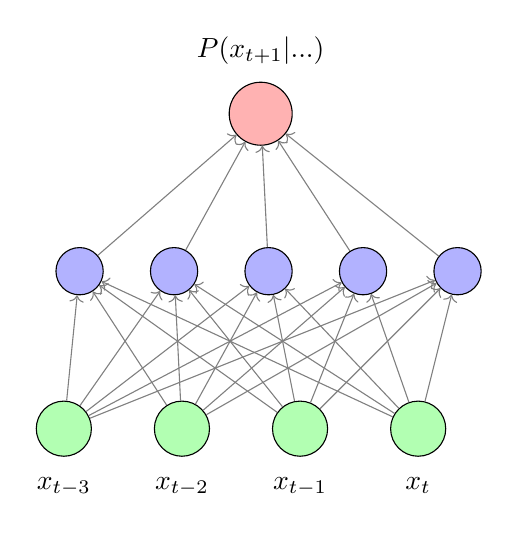
\begin{tikzpicture}[scale=1.0]
% 输入层
\foreach \i in {1,2,3,4} {
    \node[circle,draw,fill=green!30,minimum size=0.7cm] (i\i) at (\i*1.5,0) {};
}
\node[below] at (1.5,-0.5) {$x_{t-3}$};
\node[below] at (3,-0.5) {$x_{t-2}$};
\node[below] at (4.5,-0.5) {$x_{t-1}$};
\node[below] at (6,-0.5) {$x_t$};

% 隐藏层
\foreach \i in {1,2,3,4,5} {
    \node[circle,draw,fill=blue!30,minimum size=0.6cm] (h\i) at (\i*1.2+0.5,2) {};
}

% 输出层
\node[circle,draw,fill=red!30,minimum size=0.8cm] (o) at (4,4) {};
\node[above] at (4,4.5) {$P(x_{t+1}|...)$};

% 连接
\foreach \i in {1,2,3,4} {
    \foreach \j in {1,2,3,4,5} {
        \draw[->,thin,gray] (i\i) -- (h\j);
    }
}
\foreach \i in {1,2,3,4,5} {
    \draw[->,thin,gray] (h\i) -- (o);
}

\end{tikzpicture}
\end{center}

\textbf{问题:}
\begin{itemize}
    \item 输入维度固定为 $\tau$
    \item 参数数量随 $\tau$ 增长
    \item 无法处理变长序列
\end{itemize}


\paragraph{MLP语言模型的局限}
\begin{center}
\begin{tikzpicture}[scale=1.0]
% 窗口大小问题
\node[draw,fill=red!20,text width=10cm] at (5,3.5) {
\textbf{问题1:窗口大小固定}
\begin{itemize}
    \item $\tau=4$:只能看4个词
    \item 长期依赖无法捕捉
    \item ``I grew up in France... I speak fluent \_\_\_''
\end{itemize}
};

% 参数爆炸
\node[draw,fill=orange!20,text width=10cm] at (5,1.8) {
\textbf{问题2:参数数量}
\begin{itemize}
    \item 输入层:$\tau \times d_{embed}$
    \item 词表大:$V=10000$,$\tau=100$ $\Rightarrow$ 百万级参数
\end{itemize}
};

% 无法共享
\node[draw,fill=yellow!20,text width=10cm] at (5,0.3) {
\textbf{问题3:无法参数共享}
\begin{itemize}
    \item 处理位置1和位置2的``the''用不同参数
\end{itemize}
};

\end{tikzpicture}
\end{center}


\paragraph{需要一个"记忆装置"}
\textbf{核心思想:}引入\textbf{隐状态}作为记忆

\begin{center}
\begin{tikzpicture}[scale=1.1]
% 对比
\node[text width=4.5cm,align=center] at (2,3.5) {
\textbf{MLP:无记忆}
};

\node[text width=4.5cm,align=center] at (8,3.5) {
\textbf{RNN:有记忆}
};

% MLP
\foreach \i in {1,2,3} {
    \node[circle,draw,fill=blue!20,minimum size=0.5cm] (m\i) at (\i*0.8,2) {};
}
\node[circle,draw,fill=green!30,minimum size=0.6cm] at (1.6,1) {输出};
\draw[->,thick] (m1) -- (1.6,1.3);
\draw[->,thick] (m2) -- (1.6,1.3);
\draw[->,thick] (m3) -- (1.6,1.3);
\node[below,font=\tiny,text width=3cm,align=center] at (1.6,0.5) {每次重新开始};

% RNN
\node[circle,draw,fill=red!20,minimum size=0.6cm] (h1) at (6.5,2) {$h_1$};
\node[circle,draw,fill=red!20,minimum size=0.6cm] (h2) at (7.5,2) {$h_2$};
\node[circle,draw,fill=red!20,minimum size=0.6cm] (h3) at (8.5,2) {$h_3$};
\node[circle,draw,fill=red!20,minimum size=0.6cm] (h4) at (9.5,2) {$h_4$};

\draw[->,thick,blue] (h1) -- (h2);
\draw[->,thick,blue] (h2) -- (h3);
\draw[->,thick,blue] (h3) -- (h4);
\node[below,font=\tiny,text width=3cm,align=center] at (8,0.5) {隐状态记住历史};

\end{tikzpicture}
\end{center}

\begin{theorem}[关键]
隐状态 $h_t$ 总结了到时刻 $t$ 为止的所有历史信息
\end{theorem}



\subsection{有隐状态的循环神经网络}

\subsection{8.4.2 有隐状态的循环神经网络}

\subsection{8.4.2 有隐状态的循环神经网络}
\begin{center}
\Large \textcolor{blue}{RNN的核心:循环连接}
\end{center}


\paragraph{RNN的基本结构}
\textbf{核心思想:}隐状态在时间步之间传递

\begin{definition}[数学定义]
\begin{align*}
\mathbf{H}_t &= \phi(\mathbf{X}_t \mathbf{W}_{xh} + \mathbf{H}_{t-1}\mathbf{W}_{hh} + \mathbf{b}_h) \\
\mathbf{O}_t &= \mathbf{H}_t \mathbf{W}_{hq} + \mathbf{b}_q
\end{align*}
\end{definition}

\textbf{符号说明:}
\begin{itemize}
    \item $\mathbf{X}_t \in \mathbb{R}^{n \times d}$:时间步 $t$ 的输入($n$ 个样本)
    \item $\mathbf{H}_t \in \mathbb{R}^{n \times h}$:隐状态($h$ 是隐藏单元数)
    \item $\mathbf{O}_t \in \mathbb{R}^{n \times q}$:输出($q$ 是输出维度)
    \item $\mathbf{W}_{xh} \in \mathbb{R}^{d \times h}$:输入到隐藏的权重
    \item $\mathbf{W}_{hh} \in \mathbb{R}^{h \times h}$:隐藏到隐藏的权重
    \item $\mathbf{W}_{hq} \in \mathbb{R}^{h \times q}$:隐藏到输出的权重
    \item $\phi$:激活函数(通常是 $\tanh$)
\end{itemize}


\paragraph{RNN的计算图}
\begin{center}
\begin{tikzpicture}[scale=1.2]
% 隐藏层
\foreach \i in {1,2,3,4} {
    \node[circle,draw,fill=red!20,minimum size=1cm] (h\i) at (\i*2.5,2) {$\mathbf{H}_{\i}$};
}

% 输入层
\foreach \i in {1,2,3,4} {
    \node[circle,draw,fill=green!20,minimum size=0.8cm] (x\i) at (\i*2.5,0) {$\mathbf{X}_{\i}$};
}

% 输出层
\foreach \i in {1,2,3,4} {
    \node[circle,draw,fill=blue!20,minimum size=0.8cm] (o\i) at (\i*2.5,4) {$\mathbf{O}_{\i}$};
}

% 连接
\foreach \i in {1,2,3,4} {
    \draw[->,thick] (x\i) -- (h\i) node[midway,right,font=\tiny] {$\mathbf{W}_{xh}$};
    \draw[->,thick] (h\i) -- (o\i) node[midway,right,font=\tiny] {$\mathbf{W}_{hq}$};
}

% 循环连接
\foreach \i in {1,2,3} {
    \pgfmathtruncatemacro{\next}{\i+1}
    \draw[->,very thick,blue] (h\i) -- (h\next) node[midway,above,font=\tiny] {$\mathbf{W}_{hh}$};
}

% 标注
\node[below] at (5,-0.7) {\textbf{关键:}相同的权重在所有时间步共享!};

\end{tikzpicture}
\end{center}


\paragraph{RNN的展开视图}
\textbf{将循环展开成前馈网络:}

\begin{center}
\begin{tikzpicture}[scale=0.9]
% 折叠视图
\node[draw,fill=yellow!20,text width=3cm,align=center] at (0,2) {
\textbf{折叠视图}\\
循环结构
};

\node[circle,draw,fill=red!20,minimum size=1cm] (h) at (0,0) {$\mathbf{H}$};
\node[circle,draw,fill=green!20] (x) at (-1.5,-1.5) {$\mathbf{X}$};
\node[circle,draw,fill=blue!20] (o) at (1.5,-1.5) {$\mathbf{O}$};

\draw[->,thick] (x) -- (h);
\draw[->,thick] (h) -- (o);
\draw[->,thick,blue] (h) to[out=135,in=45,looseness=8] (h);

% 箭头
\draw[->,ultra thick] (2,0) -- (4,0) node[midway,above] {展开};

% 展开视图
\node[draw,fill=yellow!20,text width=3cm,align=center] at (9,2) {
\textbf{展开视图}\\
前馈网络
};

\foreach \i in {1,2,3} {
    \node[circle,draw,fill=red!20,minimum size=0.8cm] (H\i) at (5+\i*1.5,0) {$\mathbf{H}_{\i}$};
    \node[circle,draw,fill=green!20,minimum size=0.6cm] (X\i) at (5+\i*1.5,-1.5) {$\mathbf{X}_{\i}$};
    \node[circle,draw,fill=blue!20,minimum size=0.6cm] (O\i) at (5+\i*1.5,1.5) {$\mathbf{O}_{\i}$};
    
    \draw[->,thick] (X\i) -- (H\i);
    \draw[->,thick] (H\i) -- (O\i);
}

\draw[->,thick,blue] (H1) -- (H2);
\draw[->,thick,blue] (H2) -- (H3);

\end{tikzpicture}
\end{center}

\begin{theorem}[关键特点]
\begin{itemize}
    \item 展开后是一个很深的网络(深度=序列长度)
    \item 所有时间步\textbf{共享相同的参数} $\mathbf{W}_{xh}, \mathbf{W}_{hh}, \mathbf{W}_{hq}$
\end{itemize}
\end{theorem}


\paragraph{RNN的参数共享}
\textbf{为什么参数共享?}

\begin{center}
\begin{tikzpicture}[scale=1.0]
% 时间步1
\node[draw,fill=blue!20,minimum size=1cm] (h1) at (0,2) {$\mathbf{H}_1$};
\node[draw,fill=green!20] (x1) at (0,0.5) {$\mathbf{X}_1$};
\draw[->,thick] (x1) -- (h1) node[midway,right,font=\tiny,red] {$\mathbf{W}_{xh}$};

% 时间步2
\node[draw,fill=blue!20,minimum size=1cm] (h2) at (3,2) {$\mathbf{H}_2$};
\node[draw,fill=green!20] (x2) at (3,0.5) {$\mathbf{X}_2$};
\draw[->,thick] (x2) -- (h2) node[midway,right,font=\tiny,red] {$\mathbf{W}_{xh}$};
\draw[->,thick] (h1) -- (h2) node[midway,above,font=\tiny,red] {$\mathbf{W}_{hh}$};

% 时间步3
\node[draw,fill=blue!20,minimum size=1cm] (h3) at (6,2) {$\mathbf{H}_3$};
\node[draw,fill=green!20] (x3) at (6,0.5) {$\mathbf{X}_3$};
\draw[->,thick] (x3) -- (h3) node[midway,right,font=\tiny,red] {$\mathbf{W}_{xh}$};
\draw[->,thick] (h2) -- (h3) node[midway,above,font=\tiny,red] {$\mathbf{W}_{hh}$};

% 标注
\node[below,text width=8cm,align=center,font=\small] at (3,-0.5) {
\textcolor{red}{相同的权重} $\Rightarrow$ 处理``the''用同样的变换
};

\end{tikzpicture}
\end{center}

\textbf{优点:}
\begin{itemize}
    \item $\checkmark$ 参数数量与序列长度无关
    \item $\checkmark$ 可以处理任意长度的序列
    \item $\checkmark$ 学到的模式可以迁移到序列的任何位置
\end{itemize}


\paragraph{RNN的前向传播过程}
\textbf{逐步计算:}

\begin{enumerate}
    \item \textbf{初始化:}$\mathbf{H}_0 = \mathbf{0}$(或学习得到)
    
    \item \textbf{时间步1:}
    \begin{align*}
    \mathbf{H}_1 &= \tanh(\mathbf{X}_1 \mathbf{W}_{xh} + \mathbf{H}_0 \mathbf{W}_{hh} + \mathbf{b}_h) \\
    \mathbf{O}_1 &= \mathbf{H}_1 \mathbf{W}_{hq} + \mathbf{b}_q
    \end{align*}
    
    \item \textbf{时间步2:}
    \begin{align*}
    \mathbf{H}_2 &= \tanh(\mathbf{X}_2 \mathbf{W}_{xh} + \mathbf{H}_1 \mathbf{W}_{hh} + \mathbf{b}_h) \\
    \mathbf{O}_2 &= \mathbf{H}_2 \mathbf{W}_{hq} + \mathbf{b}_q
    \end{align*}
    
    \item \textbf{...重复...}
\end{enumerate}

\begin{theorem}[关键]
每一步都依赖前一步的隐状态 $\mathbf{H}_{t-1}$
\end{theorem}


\paragraph{激活函数的选择}
\textbf{为什么用 $\tanh$?}

\begin{center}
\begin{tikzpicture}[scale=1.0]
% 坐标轴
\draw[->,thick] (-3,0) -- (3,0) node[right] {$x$};
\draw[->,thick] (0,-1.5) -- (0,1.5) node[above] {$y$};

% tanh曲线
\draw[blue,thick,domain=-2.5:2.5,samples=100] plot (\x,{tanh(\x)});
\node[blue,right] at (2,1) {$\tanh(x)$};

% 标注
\draw[dashed] (-3,1) -- (3,1);
\draw[dashed] (-3,-1) -- (3,-1);
\node[left] at (0,1) {1};
\node[left] at (0,-1) {-1};

% 特点
\node[below,text width=6cm,align=center] at (0,-2.2) {
\small 输出范围:$[-1, 1]$ | 平滑 | 零中心
};

\end{tikzpicture}
\end{center}



\textbf{优点:}
\begin{itemize}
    \item 输出有界
    \item 零中心(mean=0)
    \item 梯度更稳定
\end{itemize}


\textbf{也可以用:}
\begin{itemize}
    \item ReLU:计算快
    \item sigmoid:$[0,1]$输出
    \item 但 $\tanh$ 最常用
\end{itemize}



\paragraph{RNN前向传播代码}
\begin{lstlisting}
def rnn_forward(inputs, state, params):
    """ inputs: sequence,shape (batch_size, vocab_size) state: (batch_size, num_hiddens) params: [W_xh, W_hh, b_h, W_hq, b_q] """
    W_xh, W_hh, b_h, W_hq, b_q = params
    outputs = []
    H = state
    
    for X in inputs:
        H = torch.tanh(torch.mm(X, W_xh) + torch.mm(H, W_hh) + b_h)
        # Output
        Y = torch.mm(H, W_hq) + b_q
        outputs.append(Y)
    
    return torch.cat(outputs, dim=0), H
\end{lstlisting}

\begin{definition}[关键点]
\begin{itemize}
    \item 循环遍历每个时间步
    \item 隐状态 $H$ 不断更新
    \item 返回所有输出和最终隐状态
\end{itemize}
\end{definition}


\paragraph{隐状态的继续输出}
\textbf{维度分析}

\begin{definition}[重要:理解各个张量的形状]
\begin{center}
\begin{tabular}{|l|c|l|}
\hline
\textbf{变量} & \textbf{形状} & \textbf{说明} \\
\hline
$\mathbf{X}_t$ & $(n, d)$ & 批量大小$n$,输入维度$d$ \\
\hline
$\mathbf{H}_t$ & $(n, h)$ & 批量大小$n$,隐藏单元数$h$ \\
\hline
$\mathbf{W}_{xh}$ & $(d, h)$ & 输入到隐藏 \\
\hline
$\mathbf{W}_{hh}$ & $(h, h)$ & 隐藏到隐藏 \\
\hline
$\mathbf{W}_{hq}$ & $(h, q)$ & 隐藏到输出 \\
\hline
$\mathbf{b}_h$ & $(h,)$ & 隐藏层偏置 \\
\hline
$\mathbf{b}_q$ & $(q,)$ & 输出层偏置 \\
\hline
\end{tabular}
\end{center}

\begin{example}[示例]
批量大小 $n=32$,输入维度 $d=256$,隐藏单元 $h=128$,输出维度 $q=100$
\end{example}
\end{definition}



\subsection{基于循环神经网络的字符级语言模型}

\subsection{8.4.3 基于循环神经网络的字符级语言模型}

\subsection{8.4.3 基于循环神经网络的字符级语言模型}
\textbf{目标:}用RNN构建字符级语言模型

\begin{center}
\Large \textcolor{blue}{实现一个能生成文本的RNN模型}
\end{center}


\paragraph{字符级语言模型}
\begin{center}
\begin{tikzpicture}[scale=1.0]
% MLP
\node[draw,fill=blue!20] at (0,2) {\textbf{任务:}预测下一个字符};

% 输入序列
\node[font=\small] at (-1.5,3) {\textbf{MLP(窗口$\tau=100$)}};
\foreach \i/\c in {0/t,1/h,2/e,3/{ },4/t,5/i,6/m,7/e} {
    \node[draw,fill=green!20,minimum size=0.6cm] at (\i*0.8,2) {\tiny\c};
}

% RNN处理
\node[font=\small] at (-1,1.5) {\textbf{RNN}};
\node[draw,fill=green!20,text width=4.5cm] at (6,2.5) {
\textbf{RNN}\\
$\mathbf{W}_{xh}$:$d \times h$\\
$\mathbf{W}_{hh}$:$h \times h$\\
$\mathbf{W}_{hq}$:$h \times V$\\
\textcolor{green!60!black}{\textbf{总计:固定!}}
};

% 箭头
\foreach \i in {0,...,6} {
    \pgfmathtruncatemacro{\next}{\i+1}
    \draw[->,thick,blue] (\i*0.8,2) -- (\next*0.8,2);
}

% 输出预测
\node[font=\small] at (-1,0.5) {预测:};
\foreach \i/\c in {1/h,2/e,3/{ },4/t,5/i,6/m,7/e} {
    \node[draw,fill=red!20,minimum size=0.6cm] at (\i*0.8,0) {\c};
}

% 连接
\foreach \i in {0,...,6} {
    \draw[->,thick] (\i*0.8,1.8) -- (\i*0.8,0.2);
}
\node[left] at (5,2.3) {序列越长};
\node[below] at (6,0) {\textcolor{green!60!black}{参数不变}};

\end{tikzpicture}
\end{center}

\begin{definition}[RNN的优势]
参数共享使得RNN可以高效处理任意长度的序列
\end{definition}

\paragraph{字符级语言模型}
\begin{center}
\Large \textcolor{blue}{给定``the''预测``h'',给定``th''预测``e''...}
\end{center}

\begin{theorem}[关键思想]
每个时间步都进行预测,使用\textbf{teacher forcing}训练
\end{theorem}


\paragraph{One-Hot编码}
\textbf{字符 $\rightarrow$ 向量}

\begin{center}
\begin{tabular}{|c|c|}
\hline
\textbf{字符} & \textbf{One-Hot向量} \\
\hline
'a' & $[1,0,0,0,0]$ \\
\hline
'b' & $[0,1,0,0,0]$ \\
\hline
'c' & $[0,0,1,0,0]$ \\
\hline
'd' & $[0,0,0,1,0]$ \\
\hline
'e' & $[0,0,0,0,1]$ \\
\hline
\end{tabular}
\end{center}

\begin{definition}[特点]
\begin{itemize}
\item 向量维度 = 词汇表大小
\item 每个向量只有一个1,其余为0
\item 稀疏表示,计算效率低
\end{itemize}
\end{definition}



\subsection{困惑度}


\subsection{8.4.4 困惑度}

\subsection{8.4.4 困惑度(Perplexity)}
\textbf{定义:}评估语言模型性能的指标

$$\textbf{PPL} = \exp\left(-\frac{1}{N}\sum_{t=1}^{N}\log p(x_t|x_{<t})\right)$$



\textbf{好的模型:}
\begin{itemize}
\item 高概率预测下一个词
\item 低困惑度
\item PPL = $\exp(0.25) \approx$ 1.3
\end{itemize}


\textbf{差的模型:}
\begin{itemize}
\item 低概率预测下一个词
\item 高困惑度
\item PPL = $\exp(2.3) \approx$ 10
\end{itemize}


\begin{theorem}[直观理解]
困惑度 = 模型在预测时的"平均选择数量"
\end{theorem}




\section{从零开始实现循环神经网络}


\section{8.5 从零开始实现循环神经网络}

\paragraph{从零实现的意义}
\begin{center}
\begin{tikzpicture}[scale=0.9]
% 两种方式
\node[draw,fill=yellow!20,rounded corners,text width=5cm,align=center] at (0,2) {
\textbf{使用框架}\\
\texttt{nn.RNN()}\\
简单快速\\
但细节不清楚
};

\node[draw,fill=green!20,rounded corners,text width=5cm,align=center] at (7,2) {
\textbf{从零实现}\\
手写每一行代码\\
理解每个细节\\
知其所以然
};

\draw[->,ultra thick,blue] (2.7,2) -- (4.3,2);
\node[above,blue] at (3.5,2.3) {本节目标};

\end{tikzpicture}
\end{center}

\begin{definition}[你将学会]
\begin{itemize}
    \item RNN的完整工作流程
    \item 梯度计算和反向传播
    \item 序列建模的技巧和tricks
    \item 为学习更复杂的模型打下基础
\end{itemize}
\end{definition}


\paragraph{One-Hot编码的优势}
\begin{definition}[为什么用One-Hot?]
\begin{itemize}
    \item 简单直观
    \item 无大小关系(不会让模型认为'a' < 'b')
    \item 与序列长度无关(参数量与序列长度无关)
\end{itemize}
\end{definition}

\begin{theorem}[与词级别的区别]
\begin{itemize}
    \item 词级别:通常几千到几万个词
    \item 字符级别:通常几十个字符
    \item 字符级别模型参数更少,训练更快
\end{itemize}
\end{theorem}


\paragraph{One-Hot编码实现}
\begin{lstlisting}[language=Python]
import torch.nn.functional as F

def get_one_hot(indices, vocab_size):
    """ one-hotvector indices: shape (N,) vocab_size: """
    one_hot = torch.zeros(len(indices), vocab_size)

    # 1
    one_hot.scatter_(1, indices.unsqueeze(1), 1)

    return one_hot

indices = torch.tensor([0, 2, 4])  # 'a', 'c', 'e'
one_hot = get_one_hot(indices, vocab_size=5)
print(one_hot)
\end{lstlisting}

\begin{definition}[输出结果]
\begin{verbatim}
tensor([[1., 0., 0., 0., 0.],  # 'a'
        [0., 0., 1., 0., 0.],  # 'c'
        [0., 0., 0., 0., 1.]]) # 'e'
\end{verbatim}
\end{definition}

\paragraph{独热编码的维度转换}
\textbf{问题:}字符是离散符号,需要转为向量

\begin{definition}[独热编码:]
输入:形状为 (batch\_size, num\_steps) 的索引 \\
输出:形状为 (num\_steps, batch\_size, vocab\_size) 的one-hot张量
\end{definition}



\begin{center}
\begin{tikzpicture}[scale=0.7]
% 字符表
\node[left] at (0,2) {词表长度为 $V$ 的向量表};

% 示例
\node[draw,fill=blue!20] at (1,1) {hello};
\draw[->,thick] (1.5,1) -- (2.5,1);

% one-hot表示
\foreach \i in {0,...,4} {
    \node[draw,minimum size=0.3cm] at (\i*0.4,0) {\tiny 0};
}
\node[draw,fill=red!20,minimum size=0.3cm] at (0,0) {\tiny 1};

\node[below] at (1,-0.5) {\small 长度为 $V$ 的向量,只有一个位置为1};
\end{tikzpicture}
\end{center}


\begin{itemize}
\item 每个字符对应一个位置
\item 便于神经网络处理
\item 但向量维度很高
\end{itemize}


\paragraph{批处理独热编码}
\begin{lstlisting}[language=Python]
import torch

# data
batch_size, num_steps, vocab_size = 2, 3, 28
X = torch.tensor([[1, 2, 3], [4, 5, 6]])  # (2, 3)

X_one_hot = get_one_hot(X, vocab_size)
print(f"shape: {X_one_hot.shape}")  # (3, 2, 28)
\end{lstlisting}

\begin{theorem}[注意]
转置是为了方便RNN按时间步处理:$(T, N, V)$
\end{theorem}

\begin{center}
\begin{tikzpicture}[scale=0.8]
% 原始数据
\node[draw,fill=blue!20] at (0,2) {$X$ (2,3)};
\node[below] at (0,1.5) {\small 批量索引};

% 转换过程
\draw[->,thick] (0.5,2) -- (2,2);
\node[above] at (1.25,2.1) {\small one-hot};

% 结果
\node[draw,fill=green!20] at (4,2) {$X_{one-hot}$ (3,2,28)};
\node[below] at (4,1.5) {\small 批量向量};
\end{tikzpicture}
\end{center}


\paragraph{RNN语言模型的完整流程}
\begin{itemize}
    \item \textbf{步骤1: 数据准备} - 文本 $\rightarrow$ 字符索引 $\rightarrow$ One-hot向量
    \item \textbf{步骤2: RNN计算} - 循环神经网络处理序列
    \item \textbf{步骤3: 输出预测} - 计算下一个字符的概率分布
    \item \textbf{步骤4: 采样} - 根据概率选择下一个字符
\end{itemize}


\paragraph{步骤3: 输出预测}
\begin{itemize}
    \item 向输出层:$\mathbf{O}_t = \mathbf{H}_t \mathbf{W}_{hq} + \mathbf{b}_q$
    \item 输出维度 = 词表大小
    \item 稀疏表示(未归一化的logits)
\end{itemize}


\paragraph{步骤4: 采样}
根据概率分布选择下一个字符



\paragraph{独热编码实现}
\begin{lstlisting}[language=python]
import torch
import torch.nn.functional as F

def one_hot(indices, vocab_size):
    """ indices: (batch_size, num_steps) Return: (batch_size, num_steps, vocab_size) """
    return F.one_hot(indices, vocab_size).float()

# comment
vocab_size = 28  # 26个字母 + 空格 + 其他
batch_size, num_steps = 2, 5

# comment
X = torch.randint(0, vocab_size, (batch_size, num_steps))
print(f"索引形状: {X.shape}")  # (2, 5)

# comment
X_one_hot = one_hot(X, vocab_size)
print(f"独热编码形状: {X_one_hot.shape}")  # (2, 5, 28)
\end{lstlisting}


\paragraph{完整的RNN模型}
\begin{lstlisting}
class RNNModelScratch:
    def __init__(self, vocab_size, num_hiddens):
        self.vocab_size = vocab_size
        self.num_hiddens = num_hiddens
        
        #  comment
        self.params = self.init_params()
    
    def init_params(self):
        """Simple function"""
        def normal(shape):
            return torch.randn(size=shape) * 0.01
        
        # comment
        W_xh = normal((self.vocab_size, self.num_hiddens))
        # comment
        W_hh = normal((self.num_hiddens, self.num_hiddens))
        # comment
        b_h = torch.zeros(self.num_hiddens)
        # comment
        W_hq = normal((self.num_hiddens, self.vocab_size))
        # comment
        b_q = torch.zeros(self.vocab_size)
        
        # comment
        params = [W_xh, W_hh, b_h, W_hq, b_q]
        for param in params:
            param.requires_grad_(True)
        
        return params
\end{lstlisting}


\paragraph{完整的字符级RNN语言模型}
\begin{center}
\begin{tikzpicture}[scale=0.9]
% RNN流程图
\node[draw,fill=yellow!20,rounded corners,text width=10cm,align=center] at (5,3) {
\textbf{输入:}字符序列 $\to$ 独热编码
};

\draw[->,thick] (5,2.5) -- (5,2);

\node[draw,fill=blue!20,rounded corners,text width=10cm,align=center] at (5,1.5) {
\textbf{RNN层:}循环更新隐状态\\
$\mathbf{H}_t = \tanh(\mathbf{X}_t \mathbf{W}_{xh} + \mathbf{H}_{t-1}\mathbf{W}_{hh} + \mathbf{b}_h)$
};

\draw[->,thick] (5,1) -- (5,0.5);

\node[draw,fill=green!20,rounded corners,text width=10cm,align=center] at (5,0) {
\textbf{输出层:}预测下一个字符\\
$\mathbf{O}_t = \mathbf{H}_t \mathbf{W}_{hq} + \mathbf{b}_q$
};

\end{tikzpicture}
\end{center}

\begin{theorem}[目标]
最大化正确字符的预测概率
\end{theorem}


\paragraph{字符级模型的优缺点}


\textcolor{blue}{\textbf{优点:}}
\begin{itemize}
    \item $\checkmark$ 词表很小($\sim$100)
    \item $\checkmark$ 无OOV问题
    \item $\checkmark$ 可以生成任意词
    \item $\checkmark$ 适合演示和教学
\end{itemize}

\textbf{适用场景:}
\begin{itemize}
    \item 拼写纠错
    \item 文本生成
    \item DNA序列分析
\end{itemize}


\textcolor{red}{\textbf{缺点:}}
\begin{itemize}
    \item $\times$ 序列很长
    \item $\times$ 训练慢
    \item $\times$ 需要更多计算
    \item $\times$ 难以捕捉长期依赖
\end{itemize}

\textbf{实际应用:}
\begin{itemize}
    \item 现代NLP多用词级或子词级
\end{itemize}



\paragraph{训练循环}
\begin{lstlisting}
def train_epoch(model, train_iter, loss_fn, optimizer):
    """epoch"""
    total_loss = 0
    num_batches = 0
    
    for X, Y in train_iter:
        # X, Y: (batch_size, num_steps)
        
        # One-hot编码
        inputs = get_one_hot(X, model.vocab_size)
        # inputs: (num_steps, batch_size, vocab_size)
        
        # comment
        state = model.init_state(X.shape[0])
        
        # comment
        outputs, state = model.forward(inputs, state)
        # outputs: (num_steps * batch_size, vocab_size)
        
        # comment
        Y = Y.T.reshape(-1)  # (num_steps * batch_size,)
        loss = loss_fn(outputs, Y)
        
        # comment
        optimizer.zero_grad()
        loss.backward()
        # comment
        grad_clipping(model.params, 1)
        optimizer.step()
        
        total_loss += loss.item()
        num_batches += 1
    
    return total_loss / num_batches
\end{lstlisting}


\paragraph{梯度裁剪的重要性}
\textbf{问题:}RNN容易出现梯度爆炸

\begin{center}
\begin{tikzpicture}[scale=1.0]
% 梯度爆炸
\draw[->,thick] (0,0) -- (6,0) node[right] {训练步数};
\draw[->,thick] (0,0) -- (0,3) node[above] {梯度范数};

% 爆炸曲线
\draw[red,thick] (0.5,0.5) -- (1,0.6) -- (1.5,0.8) -- (2,1.5) -- (2.5,2.8);
\node[red,above] at (2.5,2.8) {爆炸!};

% 裁剪后
\draw[blue,thick] (3,0.5) -- (3.5,0.6) -- (4,0.8) -- (4.5,1.0) -- (5,1.0) -- (5.5,0.9);
\draw[dashed,green!60!black] (0,1) -- (6,1);
\node[green!60!black,left] at (0,1) {阈值};
\node[blue,above] at (5,1.2) {裁剪后稳定};

\end{tikzpicture}
\end{center}

\begin{definition}[梯度裁剪]
$$\mathbf{g} \leftarrow \min\left(1, \frac{\theta}{\|\mathbf{g}\|}\right) \mathbf{g}$$
其中 $\theta$ 是阈值(通常取1或5)
\end{definition}


\paragraph{困惑度与交叉熵的关系}

\begin{center}
\begin{tikzpicture}[scale=1.0]
% 坐标轴
\draw[->,thick] (0,0) -- (6,0) node[right] {交叉熵};
\draw[->,thick] (0,0) -- (0,4) node[above] {困惑度};

% 指数曲线
\draw[blue,thick,domain=0:3.5,samples=100] plot (\x,{exp(\x*0.6)});

% 标注点
\fill[red] (1,1.82) circle (2pt);
\node[red,above right] at (1,1.82) {CE=1, PPL$\approx$ 2-3};

% 高困惑度
\fill[red] (2,3.32) circle (2pt);
\node[red,above right] at (2,3.32) {CE=2, PPL$=e^2\approx$7.4};

% 公式
\node[below,text width=6cm,align=center] at (3,-0.8) {
$\text{PPL} = \exp(\text{CE})$
};

\end{tikzpicture}
\end{center}

\begin{theorem}[注意]
困惑度对交叉熵的微小差异很敏感(指数关系)
\end{theorem}


\paragraph{困惑度的意义}
\begin{definition}[直观理解]
困惑度告诉我们:在每一步,模型平均在多少个选项之间``困惑''
\end{definition}

\begin{example}[示例]
\begin{itemize}
    \item PPL = 2:模型在2个选项间困惑
    \item PPL = 28:模型在28个字符间困惑(相当于随机猜)
    \item PPL = 1.5:模型比较确定
\end{itemize}
\end{example}


\paragraph{计算困惑度}
\begin{lstlisting}
def evaluate_perplexity(model, data_iter):
    """modeldata"""
    model.eval()
    total_loss = 0
    total_tokens = 0
    
    with torch.no_grad():
        for X, Y in data_iter:
            # One-hot编码
            inputs = get_one_hot(X, model.vocab_size)
            state = model.init_state(X.shape[0])
            
            outputs, state = model.forward(inputs, state)
            # output: (num_steps * batch_size, vocab_size)
            
            # loss
            Y = Y.T.reshape(-1)
            loss = F.cross_entropy(outputs, Y, reduction='sum')
            
            total_loss += loss.item()
            total_tokens += Y.numel()
    
    # comment = exp(平均交叉熵)
    perplexity = math.exp(total_loss / total_tokens)
    return perplexity

# comment
ppl = evaluate_perplexity(model, test_iter)
print(f"test集困惑度: {ppl:.2f}")
\end{lstlisting}


\paragraph{困惑度的实际意义}
\textbf{困惑度 = 平均分支因子}

\begin{center}
\begin{tikzpicture}[scale=0.9]
% PPL = 2
\node[circle,draw,fill=blue!20] at (0,2) {当前};
\draw[->,thick] (0.5,2) -- (1.5,2.5);
\draw[->,thick] (0.5,2) -- (1.5,1.5);
\node[circle,draw,fill=green!20] at (2,2.5) {选项1};
\node[circle,draw,fill=green!20] at (2,1.5) {选项2};
\node[below] at (1,0.5) {PPL = 2:在2个选项间困惑};

% PPL = 4
\node[circle,draw,fill=blue!20] at (5,2) {当前};
\draw[->,thick] (5.5,2) -- (6.5,3);
\draw[->,thick] (5.5,2) -- (6.5,2.3);
\draw[->,thick] (5.5,2) -- (6.5,1.7);
\draw[->,thick] (5.5,2) -- (6.5,1);
\node[circle,draw,fill=orange!20,scale=0.6] at (7,3) {1};
\node[circle,draw,fill=orange!20,scale=0.6] at (7,2.3) {2};
\node[circle,draw,fill=orange!20,scale=0.6] at (7,1.7) {3};
\node[circle,draw,fill=orange!20,scale=0.6] at (7,1) {4};
\node[below] at (6,0.5) {PPL = 4:在4个选项间困惑};
\end{tikzpicture}
\end{center}


\paragraph{困惑度的实际值}
\textbf{不同模型的困惑度范围:}

\begin{center}
\begin{tabular}{|l|c|c|}
\hline
\textbf{模型} & \textbf{数据集} & \textbf{PPL} \\
\hline
随机模型 & 任意 & $\sim$ 词表大小 \\
\hline
N-gram (n=3) & Penn Treebank & $\sim$140 \\
\hline
简单RNN & Penn Treebank & $\sim$120 \\
\hline
LSTM & Penn Treebank & $\sim$80 \\
\hline
LSTM + 正则化 & Penn Treebank & $\sim$60 \\
\hline
Transformer (大) & Penn Treebank & $\sim$20-30 \\
\hline
GPT-3 & 网络文本 & $\sim$20 \\
\hline
\end{tabular}
\end{center}

\vspace{0.3cm}
\begin{theorem}[注意]
\begin{itemize}
    \item 不同数据集的PPL不具可比性
    \item 字符级模型的PPL通常更低(词表小)
    \item PPL是相对指标,越低越好
    \item PPL=4:平均4个选择
\end{itemize}
\end{theorem}


\paragraph{困惑度与准确率的关系}
\begin{definition}[解释]
\begin{center}
\begin{tikzpicture}[scale=1.0]
% 坐标轴
\draw[->,thick] (0,0) -- (8,0) node[right] {训练epoch};
\draw[->,thick] (0,0) -- (0,4) node[above] {PPL};

% 困惑度曲线(下降)
\draw[blue,thick,domain=0:7,samples=50] plot (\x,{3.5*exp(-0.3*\x)+0.5});
\node[blue,right] at (7,1) {困惑度};

\end{tikzpicture}
\end{center}
\end{definition}


\paragraph{训练过程中的困惑度变化}
\begin{center}
\begin{tikzpicture}[scale=1.0]
% 坐标轴
\draw[->,thick] (0,0) -- (8,0) node[right] {Epoch};
\draw[->,thick] (0,0) -- (0,4) node[above] {困惑度};

% 标注区域
\fill[green!20,opacity=0.3] (0,0) rectangle (8,1.5);
\node[green!60!black] at (4,1.2) {目标区域};

% 训练集困惑度
\draw[blue,thick,domain=0.5:7.5,samples=50] plot (\x,{3.8/(\x*0.5+0.5)+0.5});

\fill[red!20,opacity=0.3] (0,2.5) rectangle (8,4);
\node[red!60!black] at (4,3.5) {训练不足};
\node[blue,right] at (7,1.5) {训练集};

% 关键点
\fill[red] (1,3.5) circle (3pt) node[above] {\tiny 开始};
\fill[green!60!black] (5,1.2) circle (3pt) node[above] {\tiny 收敛};

% 验证集困惑度
\draw[red,thick,domain=0.5:7.5,samples=50] plot (\x,{3.8/(\x*0.5+0.5)+0.2});
\node[red,right] at (7,1.5) {验证集};

% 标注
\draw[dashed] (0,1) -- (8,1);
\node[below] at (4,0.8) {\tiny 目标困惑度水平};

\end{tikzpicture}
\end{center}

\begin{definition}[训练过程]
\begin{itemize}
    \item 初期:PPL很高(模型随机猜测)
    \item 中期:PPL快速下降(学习规律)
    \item 后期:PPL缓慢下降(微调,后期趋于平稳)
    \item 最终:PPL稳定(收敛)
\end{itemize}
\end{definition}

\begin{theorem}[过拟合检测]
\begin{itemize}
    \item 训练集PPL继续下降,验证集PPL开始上升 $\to$ 过拟合
    \item 两者的PPL都稳定下降 $\to$ 训练良好
\end{itemize}
\end{theorem}


\subsection{8.4节总结}
\begin{definition}[核心概念]
\begin{enumerate}
    \item \textbf{隐状态}:记忆历史信息的向量
    \item \textbf{RNN}:通过隐状态记住历史
    \item \textbf{参数共享}:所有时间步共享权重
\end{enumerate}
\end{definition}


\subsection{8.4节总结}
\begin{definition}[数学公式]
    \textbf{无隐状态网络}:MLP无法处理变长序列
    $$\mathbf{H}_t = \phi(\mathbf{X}_t \mathbf{W}_{xh} + \mathbf{b})$$

    \textbf{RNN}:通过隐状态记住历史
    $$\mathbf{H}_t = \tanh(\mathbf{X}_t \mathbf{W}_{xh} + \mathbf{H}_{t-1} \mathbf{W}_{hh} + \mathbf{b}_h)$$

    \textbf{参数共享}:所有时间步共享权重
\end{definition}


\subsection{8.4节总结}
\begin{definition}[模型类型]
    \begin{itemize}
        \item \textbf{字符级模型}:用独热编码表示字符
        \item \textbf{词级模型}:用词嵌入表示词语
    \end{itemize}
\end{definition}

\begin{definition}[评估指标]
    \textbf{困惑度}:评估模型质量
    $$\text{PPL} = \exp\left(-\frac{1}{n}\sum_{t=1}^n \log P(x_t|x_{<t})\right)$$
\end{definition}


\paragraph{RNN的关键特性}
\begin{center}
\begin{tikzpicture}[scale=0.9]
% 特性1
\node[draw,fill=blue!20,text width=9cm] at (5,3.5) {
\textbf{1. 参数共享}\\
$\mathbf{W}_{xh}, \mathbf{W}_{hh}, \mathbf{W}_{hy}$ 在所有时间步共享
};
\end{tikzpicture}
\end{center}


\paragraph{RNN的优缺点}


\textcolor{blue}{\textbf{优点:}}
\begin{itemize}
    \item $\checkmark$ 能处理变长序列
    \item $\checkmark$ 参数共享,所有时间步复用泛化好
    \item $\checkmark$ 参数量与序列长度无关
\end{itemize}


\textcolor{red}{\textbf{缺点:}}
\begin{itemize}
    \item $\times$ 梯度消失/爆炸问题
    \item $\times$ 长距离依赖建模困难
    \item $\times$ 无法并行计算(必须按顺序)
\end{itemize}



\paragraph{RNN的关键特性}
\begin{center}
\begin{tikzpicture}[scale=0.9]
% 特性2
\node[draw,fill=green!20,text width=9cm] at (5,2.2) {
\textbf{2. 顺序处理}\\
必须按顺序处理:$\mathbf{H}_1 \rightarrow \mathbf{H}_2 \rightarrow \mathbf{H}_3$\\
$\Rightarrow$ 参数数量固定,与序列长度无关
};

% 特性3
\node[draw,fill=orange!20,text width=9cm] at (5,0.9) {
\textbf{3. 理论上的记忆能力}\\
隐状态 $\mathbf{H}_t$ 可以编码所有历史\\
$\Rightarrow$ 但实际受限于梯度消失/爆炸
};
\end{tikzpicture}
\end{center}

\begin{theorem}[下一步]
8.5节将从零实现RNN,深入理解其工作机制
\end{theorem}


\paragraph{RNN的应用场景}


\textbf{适合RNN的任务:}
\begin{itemize}
    \item 语言建模
    \item 机器翻译
    \item 语音识别
    \item 时间序列预测
    \item 视频分析
\end{itemize}


\textbf{RNN的挑战:}
\begin{itemize}
    \item 梯度消失/爆炸
    \item 长期依赖问题
    \item 训练慢(顺序处理)
    \item 难以并行
\end{itemize}


\vspace{0.5cm}
\begin{definition}[改进方向]
\begin{itemize}
    \item LSTM/GRU:解决梯度问题(第9章)
    \item 注意力机制:捕捉长期依赖
    \item Transformer:完全并行化(后续章节)
\end{itemize}
\end{definition}


latex
\paragraph{从理论到实践}
\begin{center}
\begin{tikzpicture}[scale=1.0]
% 学习路径
\node[draw,fill=yellow!20,rounded corners,text width=2.5cm,align=center] at (0,2) {
8.1-8.3\\
理论基础
};

\draw[->,ultra thick] (1.5,2) -- (2.5,2);

\node[draw,fill=blue!20,rounded corners,text width=2.5cm,align=center] at (4,2) {
8.4\\
RNN原理
};

\draw[->,ultra thick] (5.5,2) -- (6.5,2);

\node[draw,fill=green!20,rounded corners,text width=2.5cm,align=center] at (8,2) {
8.5-8.6\\
RNN实现
};

\draw[->,ultra thick] (9.5,2) -- (10.5,2);

\node[draw,fill=red!20,rounded corners,text width=2.5cm,align=center] at (12,2) {
8.7\\
BPTT
};

% 标注
\node[below,text width=12cm,align=center] at (6,0.5) {
我们已经理解了RNN的\textbf{工作原理}\\
接下来将\textbf{从零实现}RNN(8.5节)
};

\end{tikzpicture}
\end{center}

\begin{definition}[已掌握的知识]
\begin{itemize}
    \item $\checkmark$ 为什么需要隐状态
    \item $\checkmark$ RNN的数学公式
    \item $\checkmark$ 参数共享机制
    \item $\checkmark$ 字符级语言模型
    \item $\checkmark$ 困惑度评估
\end{itemize}
\end{definition}


\subsection{8.4节核心公式总结}
\begin{definition}[RNN的核心公式]
\begin{align*}
\text{\textbf{隐状态更新:}} \quad & \mathbf{H}_t = \phi(\mathbf{X}_t \mathbf{W}_{xh} + \mathbf{H}_{t-1}\mathbf{W}_{hh} + \mathbf{b}_h) \\
\text{\textbf{输出计算:}} \quad & \mathbf{O}_t = \mathbf{H}_t \mathbf{W}_{hq} + \mathbf{b}_q \\
\text{\textbf{概率预测:}} \quad & P(x_{t+1}) = \text{softmax}(\mathbf{O}_t) \\
\text{\textbf{困惑度:}} \quad & \text{PPL} = \exp\left(-\frac{1}{n}\sum_{t=1}^{n}\log P(x_t \mid x_{<t})\right)
\end{align*}
\end{definition}

\begin{theorem}[关键要点]
\begin{itemize}
    \item 隐状态 $\mathbf{H}_t$ 携带历史信息
    \item 参数 $\mathbf{W}_{xh}, \mathbf{W}_{hh}, \mathbf{W}_{hq}$ 在所有时间步共享
    \item 激活函数通常使用 $\tanh$
    \item 困惑度越低,模型越好
\end{itemize}
\end{theorem}


\paragraph{RNN与传统模型对比}
\begin{center}
\begin{tabular}{|l|c|c|c|}
\hline
\textbf{特性} & \textbf{N-gram} & \textbf{MLP} & \textbf{RNN} \\
\hline
处理变长序列 & $\times$ & $\times$ & $\checkmark$ \\
\hline
参数数量 & 随$\tau$指数增长 & 随$\tau$线性增长 & 固定 \\
\hline
长期依赖 & 受限于$\tau$ & 受限于$\tau$ & 理论上可以 \\
\hline
并行化 & $\checkmark$ & $\checkmark$ & $\times$ \\
\hline
参数共享 & $\times$ & $\times$ & $\checkmark$ \\
\hline
训练难度 & 简单 & 中等 & 较难 \\
\hline
\end{tabular}
\end{center}

\vspace{0.5cm}
\begin{definition}[RNN的核心优势]
通过\textbf{隐状态}和\textbf{参数共享},实现了用固定参数处理任意长度序列
\end{definition}


\paragraph{训练RNN的关键技巧}


\textbf{1. 梯度裁剪}
\begin{itemize}
    \item 防止梯度爆炸
    \item 阈值通常取1或5
    \item 必不可少!
\end{itemize}

\textbf{2. 隐状态初始化}
\begin{itemize}
    \item 零初始化
    \item 可学习初始化
    \item 使用前一批次的隐状态
\end{itemize}


\textbf{3. 序列采样}
\begin{itemize}
    \item 随机采样:简单
    \item 顺序分区:效果好
    \item 保持隐状态连续性
\end{itemize}

\textbf{4. 学习率调整}
\begin{itemize}
    \item 从较小值开始
    \item 使用学习率衰减
    \item 监控梯度范数
\end{itemize}


\vspace{0.5cm}
\begin{theorem}[经验]
RNN训练需要仔细调参,梯度裁剪是关键!
\end{theorem}


\paragraph{常见问题与解决方案}
\begin{center}
\begin{tikzpicture}[scale=0.9]
% 问题1
\node[draw,fill=red!20,text width=5cm] at (0,3.5) {
\textbf{问题1:梯度爆炸}\\
梯度突然变得很大
};
\node[draw,fill=green!20,text width=5cm] at (6,3.5) {
\textbf{解决:}\\
梯度裁剪 + 小学习率
};
\draw[->,thick] (2.7,3.5) -- (3.8,3.5);

% 问题2
\node[draw,fill=red!20,text width=5cm] at (0,2.2) {
\textbf{问题2:梯度消失}\\
长期依赖学不到
};
\node[draw,fill=green!20,text width=5cm] at (6,2.2) {
\textbf{解决:}\\
使用LSTM/GRU(第9章)
};
\draw[->,thick] (2.7,2.2) -- (3.8,2.2);

% 问题3
\node[draw,fill=red!20,text width=5cm] at (0,0.9) {
\textbf{问题3:训练慢}\\
顺序处理效率低
};
\node[draw,fill=green!20,text width=5cm] at (6,0.9) {
\textbf{解决:}\\
截断BPTT + GPU加速
};
\draw[->,thick] (2.7,0.9) -- (3.8,0.9);

\end{tikzpicture}
\end{center}


\subsection{8.4节思维导图}
\begin{center}
\begin{tikzpicture}[scale=0.75,
    box/.style={rectangle,draw,fill=blue!20,rounded corners,text width=2.3cm,align=center,minimum height=0.8cm}]

% 中心
\node[box,fill=yellow!30,text width=3cm] (center) at (6,3) {\textbf{8.4 RNN原理}};

% 四个主要分支
\node[box] (no) at (0,5) {8.4.1\\无隐状态\\网络};
\node[box] (yes) at (4,5.5) {8.4.2\\有隐状态\\RNN};
\node[box] (char) at (8,5.5) {8.4.3\\字符级\\语言模型};
\node[box] (ppl) at (12,5) {8.4.4\\困惑度};

% 连接
\draw[->,thick] (center) -- (no);
\draw[->,thick] (center) -- (yes);
\draw[->,thick] (center) -- (char);
\draw[->,thick] (center) -- (ppl);

% 细节
\node[font=\tiny,text width=2.5cm,align=center] at (0,3.8) {MLP无法\\处理变长序列};
\node[font=\tiny,text width=2.5cm,align=center] at (4,3.8) {隐状态记忆\\参数共享};
\node[font=\tiny,text width=2.5cm,align=center] at (8,3.8) {One-hot编码\\预测下一字符};
\node[font=\tiny,text width=2.5cm,align=center] at (12,3.8) {评估指标\\PPL=exp(CE)};

% 关键公式
\node[draw,fill=green!20,text width=10cm,font=\small] at (6,1) {
\textbf{核心公式:}$\mathbf{H}_t = \tanh(\mathbf{X}_t \mathbf{W}_{xh} + \mathbf{H}_{t-1}\mathbf{W}_{hh} + \mathbf{b}_h)$
};

\end{tikzpicture}
\end{center}


\paragraph{知识检查}
\begin{definition}[问题1]
为什么RNN需要隐状态?传统MLP有什么问题?
\end{definition}

\begin{definition}[问题2]
RNN的参数数量与序列长度有关吗?为什么?
\end{definition}

\begin{definition}[问题3]
什么是困惑度?如何解释PPL=10?
\end{definition}

\begin{definition}[问题4]
为什么字符级RNN的困惑度通常比词级低?
\end{definition}

\begin{theorem}[思考]
如何解决RNN的梯度消失问题?(提示:LSTM)
\end{theorem}


\paragraph{准备进入8.5节}
\begin{center}
\Large \textcolor{blue}{从理论到实践:从零实现RNN}
\end{center}

\vspace{0.5cm}
\begin{definition}[8.4节回顾]
\begin{itemize}
    \item 理解了RNN的\textbf{核心思想}:用隐状态记忆历史
    \item 掌握了RNN的\textbf{数学原理}:前向传播公式
    \item 学会了\textbf{评估模型}:困惑度指标
\end{itemize}
\end{definition}

\begin{definition}[8.5节预告]
\begin{itemize}
    \item 从零实现RNN的每个细节
    \item 独热编码、初始化参数
    \item 前向传播、梯度裁剪
    \item 训练完整的字符级语言模型
    \item 文本生成
\end{itemize}
\end{definition}


\paragraph{第8章进度总结}
\begin{center}
\begin{tikzpicture}[scale=0.9]
% 进度条
\draw[thick,fill=gray!20] (0,2) rectangle (12,2.8);

% 已完成部分
\draw[thick,fill=green!40] (0,2) rectangle (6.5,2.8);

% 分节标记
\foreach \x/\label in {0/8.1,3/8.2,4.5/8.3,6/8.4,9/8.5,10.5/8.6,12/8.7} {
    \draw[thick] (\x,2) -- (\x,2.8);
    \node[below,font=\tiny] at (\x,1.8) {\label};
}

% 当前位置
\draw[->,ultra thick,red] (6.5,3.5) -- (6.5,2.9);
\node[above,red] at (6.5,3.6) {当前位置};

% 标注
\node[below,text width=12cm,align=center] at (6,0.8) {
已完成:序列模型、文本预处理、语言模型、RNN原理\\
下一步:RNN从零实现(8.5)
};

\end{tikzpicture}
\end{center}


\section{8.5 循环神经网络的从零开始实现}

\subsection{8.5 循环神经网络的从零开始实现}
\begin{center}
\Large \textcolor{blue}{动手实现:从零开始构建RNN}
\end{center}


\subsection{8.5节 - 章节导航}
\begin{definition}[本节内容]
\begin{itemize}
    \item 8.5.1 独热编码
    \item 8.5.2 初始化模型参数
    \item 8.5.3 循环神经网络模型
    \item 8.5.4 预测
    \item 8.5.5 梯度裁剪
    \item 8.5.6 训练
\end{itemize}
\end{definition}

\begin{theorem}[学习目标]
\begin{enumerate}
    \item 手写独热编码函数
    \item 理解RNN参数初始化
    \item 实现RNN前向传播
    \item 生成文本预测
    \item 掌握梯度裁剪技巧
    \item 训练完整的字符级语言模型
\end{enumerate}
\end{theorem}


\paragraph{从零实现的意义}
\begin{center}
\begin{tikzpicture}[scale=0.9]
% 两种方式
\node[draw,fill=yellow!20,rounded corners,text width=5cm,align=center] at (0,2) {
\textbf{使用框架}\\
\texttt{nn.RNN()}\\
简单快速\\
但细节不清楚
};

\node[draw,fill=green!20,rounded corners,text width=5cm,align=center] at (7,2) {
\textbf{从零实现}\\
手写每一行代码\\
理解每个细节\\
知其所以然
};

\draw[->,ultra thick,blue] (2.7,2) -- (4.3,2);
\node[above,blue] at (3.5,2.3) {本节目标};

\end{tikzpicture}
\end{center}

\begin{definition}[你将学会]
\begin{itemize}
    \item 如何将文本转为张量
    \item RNN的参数有哪些,形状是什么
    \item 前向传播的每一步计算
    \item 如何生成新文本
    \item 训练的完整流程
\end{itemize}
\end{definition}



\subsection{独热编码}

\subsection{8.5.1 独热编码}

\subsection{8.5.1 独热编码}
\begin{center}
\Large \textcolor{blue}{第一步:将字符转为向量}
\end{center}


\paragraph{为什么需要独热编码?}
\textbf{问题:}神经网络只能处理数字

\begin{center}
\begin{tikzpicture}[scale=1.0]
% 字符
\node[draw,fill=yellow!20,rounded corners,text width=2.5cm,align=center] at (0,2) {
字符\\
``a''
};

\draw[->,thick,red] (1.5,2) -- (2.5,2);
\node[red,above] at (2,2.2) {\tiny \text{×}直接用?};

% 神经网络
\node[draw,fill=blue!20,rounded corners,text width=2.5cm,align=center] at (4.5,2) {
RNN\\
需要向量
};

% 解决方案
\draw[->,ultra thick] (0,1.2) -- (0,0.5);
\node[left] at (-0.3,0.85) {\tiny 编码};

\node[draw,fill=green!20,rounded corners,text width=2.5cm,align=center] at (0,0) {
向量\\
$[1,0,0,...,0]$
};

\draw[->,ultra thick,green!60!black] (1.5,0) -- (4.5,1.5);
\node[green!60!black,above] at (3,0.8) {\tiny \checkmark 独热编码};

\end{tikzpicture}
\end{center}

\begin{theorem}[核心思想]
用长度为词表大小的向量表示每个字符,只有一个位置为1,其余为0
\end{theorem}


\paragraph{独热编码详解}
\textbf{假设词表:}\texttt{vocab = {' ':0, 'a':1, 'b':2, 'c':3, 'd':4, 'e':5}}

\begin{center}
\begin{tikzpicture}[scale=0.9]
% 词表
\node[left] at (-0.5,3.5) {词表:};
\foreach \i/\c in {0/{ },1/a,2/b,3/c,4/d,5/e} {
    \node[draw,minimum size=0.5cm] at (\i*1.2,3.5) {\tiny \c};
    \node[below,font=\tiny] at (\i*1.2,3) {\i};
}

% 字符'c'
\node[left] at (-0.5,2) {字符``c''};
\node[right] at (0.5,2) {索引=3};

\draw[->,thick] (1.5,2) -- (1.5,1.5);

% 独热向量
\node[left] at (-0.5,1) {独热编码:};
\foreach \i in {0,1,2,3,4,5} {
    \ifnum\i=3
        \node[draw,fill=red!30,minimum size=0.5cm] at (\i*1.2,1) {\tiny 1};
    \else
        \node[draw,minimum size=0.5cm] at (\i*1.2,1) {\tiny 0};
    \fi
}

% 维度标注
\draw[<->,thick] (0,0.3) -- (6,0.3);
\node[below] at (3,0.1) {向量长度 = 词表大小 = 6};

\end{tikzpicture}
\end{center}

\begin{definition}[特点]
\begin{itemize}
    \item 向量维度 = 词表大小
    \item 稀疏表示:只有一个1,其余全是0
    \item 没有顺序关系:``a''和``b''距离相同
\end{itemize}
\end{definition}


\paragraph{批量独热编码}
\textbf{输入:}批量的索引矩阵

\begin{center}
\begin{tikzpicture}[scale=0.9]
% 索引矩阵
\node[left] at (-1,3) {索引矩阵:};
\node[draw,fill=yellow!20,text width=3cm,font=\small] at (2,3) {
\texttt{X = [[1, 2, 3],}\\
\texttt{      [4, 5, 0]]}\\
形状: $(2, 3)$
};

\node[below,font=\small,align=center] at (2,2.2) {
批量大小=2\\
序列长度=3
};

\draw[->,ultra thick] (2,1.8) -- (2,1.2);
\node[right] at (2.3,1.5) {\tiny 独热编码};

% 独热张量
\node[left] at (-1,0.3) {独热张量:};
\node[draw,fill=green!20,text width=4cm,font=\small,align=center] at (2.5,0.3) {
形状: $(3, 2, 6)$\\
(时间步, 批量, 词表大小)
};

\end{tikzpicture}
\end{center}

\begin{theorem}[维度变化]
$(batch\_size, num\_steps)$ $\rightarrow$ $(num\_steps, batch\_size, vocab\_size)$
\end{theorem}


\paragraph{独热编码实现 - 方法1(手动)}
\begin{lstlisting}
import torch

def one_hot_manual(X, vocab_size):
    """ X: (batch_size, num_steps) vocab_size: vocabulary Return: (num_steps, batch_size, vocab_size) """
    batch_size, num_steps = X.shape
    
    output = torch.zeros((num_steps, batch_size, vocab_size))
    
    # X: (num_steps, batch_size)
    X = X.T
    
    # 1
    for t in range(num_steps):
        for b in range(batch_size):
            idx = X[t, b]
            output[t, b, idx] = 1
    
    return output

X = torch.tensor([[1, 2, 3], [4, 5, 0]])
result = one_hot_manual(X, vocab_size=6)
print(f"shape: {result.shape}")  # (3, 2, 6)
\end{lstlisting}


\paragraph{独热编码实现 - 方法2(PyTorch)}
\begin{lstlisting}
import torch.nn.functional as F

def one_hot(X, vocab_size):
    """ PyTorch X: (batch_size, num_steps) Return: (num_steps, batch_size, vocab_size) """
    # : (num_steps, batch_size)
    X = X.T
    
    output = F.one_hot(X, vocab_size)
    
    # float32neural network
    return output.to(torch.float32)

X = torch.tensor([[1, 2, 3], [4, 5, 0]])
result = one_hot(X, vocab_size=6)
print(f"shape: {result.shape}")  # (3, 2, 6)
print(f"data类型: {result.dtype}")  # torch.float32

print(f"第1个time step,第1个样本:")
print(result[0, 0])  # [0, 1, 0, 0, 0, 0]
\end{lstlisting}

\begin{definition}[推荐]
使用PyTorch内置的\texttt{F.one\_hot},更高效!
\end{definition}


\paragraph{独热编码的优缺点}


\textcolor{blue}{\textbf{优点:}}
\begin{itemize}
    \item $\checkmark$ 简单直观
    \item $\checkmark$ 字符间无顺序假设
    \item $\checkmark$ 易于理解和实现
    \item $\checkmark$ 适合小词表
\end{itemize}

\textbf{适用场景:}
\begin{itemize}
    \item 字符级模型(词表小)
    \item 分类任务
    \item 教学演示
\end{itemize}


\textcolor{red}{\textbf{缺点:}}
\begin{itemize}
    \item $\times$ 高维稀疏
    \item $\times$ 无语义信息
    \item $\times$ 内存占用大
    \item $\times$ 无法表示相似性
\end{itemize}

\textbf{改进方案:}
\begin{itemize}
    \item 词嵌入(Word Embedding)
    \item 降维表示
    \item 预训练向量
\end{itemize}


\vspace{0.5cm}
\begin{theorem}[实际应用]
现代NLP通常用\textbf{词嵌入}代替独热编码(后续章节)
\end{theorem}


\paragraph{完整的数据准备}
\begin{lstlisting}
def prepare_data(batch_size, num_steps):
    """Prepare training data"""
    # data
    train_iter, vocab = load_data_time_machine(
        batch_size, num_steps
    )
    
    # batch
    for X, Y in train_iter:
        print(f"Xshape(索引): {X.shape}")  # (batch_size, num_steps)
        print(f"Yshape(标签): {Y.shape}")  # (batch_size, num_steps)
        
        X_one_hot = one_hot(X, len(vocab))
        print(f"X_one_hotshape: {X_one_hot.shape}")  
        # (num_steps, batch_size, vocab_size)
        
        break
    
    return train_iter, vocab

train_iter, vocab = prepare_data(batch_size=32, num_steps=35)
print(f"vocabulary大小: {len(vocab)}")
\end{lstlisting}



\subsection{初始化模型参数}

\subsection{8.5.2 初始化模型参数}

\subsection{8.5.2 初始化模型参数}
\begin{center}
\Large \textcolor{blue}{第二步:初始化RNN的权重和偏置}
\end{center}


\paragraph{RNN需要哪些参数?}
\textbf{回顾公式:}
\begin{align*}
\mathbf{H}_t &= \tanh(\mathbf{X}_t \mathbf{W}_{xh} + \mathbf{H}_{t-1}\mathbf{W}_{hh} + \mathbf{b}_h) \\
\mathbf{O}_t &= \mathbf{H}_t \mathbf{W}_{hq} + \mathbf{b}_q
\end{align*}

\begin{center}
\begin{tikzpicture}[scale=1.0]
% 参数表格
\node[draw,fill=yellow!20,text width=10cm,align=left] at (5,2) {
\textbf{需要初始化的参数:}\\
1. $\mathbf{W}_{xh}$:输入到隐藏层权重,形状 $(vocab\_size, num\_hiddens)$\\
2. $\mathbf{W}_{hh}$:隐藏层到隐藏层权重,形状 $(num\_hiddens, num\_hiddens)$\\
3. $\mathbf{b}_h$:隐藏层偏置,形状 $(num\_hiddens,)$\\
4. $\mathbf{W}_{hq}$:隐藏层到输出权重,形状 $(num\_hiddens, vocab\_size)$\\
5. $\mathbf{b}_q$:输出层偏置,形状 $(vocab\_size,)$
};

\end{tikzpicture}
\end{center}

\begin{definition}[关键]
这5个参数在\textbf{所有时间步}共享!
\end{definition}


\paragraph{参数形状分析}
\textbf{假设:}词表大小 $V=28$,隐藏单元数 $h=512$

\begin{center}
\begin{tabular}{|l|c|c|}
\hline
\textbf{参数} & \textbf{形状} & \textbf{参数量} \\
\hline
$\mathbf{W}_{xh}$ & $(28, 512)$ & 14,336 \\
\hline
$\mathbf{W}_{hh}$ & $(512, 512)$ & 262,144 \\
\hline
$\mathbf{b}_h$ & $(512,)$ & 512 \\
\hline
$\mathbf{W}_{hq}$ & $(512, 28)$ & 14,336 \\
\hline
$\mathbf{b}_q$ & $(28,)$ & 28 \\
\hline
\textbf{总计} & & \textbf{291,356} \\
\hline
\end{tabular}
\end{center}

\begin{theorem}[观察]
\begin{itemize}
    \item 大部分参数在 $\mathbf{W}_{hh}$(90\%)
    \item 与序列长度\textbf{无关}
    \item 参数量主要由 $num\_hiddens$ 决定
\end{itemize}
\end{theorem}


\paragraph{参数初始化实现}
\begin{lstlisting}
import torch

def get_params(vocab_size, num_hiddens, device):
    """ RNNparameters vocab_size: vocabulary num_hiddens: device: (CPU/GPU) """
    num_inputs = num_outputs = vocab_size
    
    def normal(shape):
        """正态分布初始化"""
        return torch.randn(size=shape, device=device) * 0.01
    
    # parameters
    W_xh = normal((num_inputs, num_hiddens))
    W_hh = normal((num_hiddens, num_hiddens))
    b_h = torch.zeros(num_hiddens, device=device)
    
    # Outputparameters
    W_hq = normal((num_hiddens, num_outputs))
    b_q = torch.zeros(num_outputs, device=device)
    
    params = [W_xh, W_hh, b_h, W_hq, b_q]
    for param in params:
        param.requires_grad_(True)
    
    return params
\end{lstlisting}


\paragraph{初始化策略详解}


\textbf{权重初始化:}
\begin{itemize}
    \item 使用\textbf{正态分布} $\mathcal{N}(0, 0.01^2)$
    \item 小的随机值
    \item 避免对称性
\end{itemize}

\textbf{为什么用0.01?}
\begin{itemize}
    \item 太大:梯度爆炸
    \item 太小:梯度消失
    \item 0.01是经验值
\end{itemize}


\textbf{偏置初始化:}
\begin{itemize}
    \item 使用\textbf{零初始化}
    \item 不影响对称性
    \item 训练中会更新
\end{itemize}

\textbf{更好的初始化:}
\begin{itemize}
    \item Xavier初始化
    \item He初始化
    \item 正交初始化(RNN常用)
\end{itemize}


\vspace{0.5cm}
\begin{theorem}[重要]
RNN对初始化敏感,建议使用\textbf{正交初始化} $\mathbf{W}_{hh}$
\end{theorem}


\paragraph{正交初始化(进阶)}
\begin{lstlisting}
def init_rnn_params_orthogonal(vocab_size, num_hiddens, device):
    """()"""
    num_inputs = num_outputs = vocab_size
    
    W_xh = torch.randn(num_inputs, num_hiddens, device=device) * 0.01
    
    W_hh = torch.eye(num_hiddens, device=device)
    #  torch.nn.init.orthogonal_(W_hh)
    
    b_h = torch.zeros(num_hiddens, device=device)
    
    # Output
    W_hq = torch.randn(num_hiddens, num_outputs, device=device) * 0.01
    b_q = torch.zeros(num_outputs, device=device)
    
    params = [W_xh, W_hh, b_h, W_hq, b_q]
    for param in params:
        param.requires_grad_(True)
    
    return params
\end{lstlisting}

\begin{definition}[优势]
正交矩阵保持梯度范数,缓解梯度消失/爆炸
\end{definition}


\paragraph{初始化隐状态}
\begin{lstlisting}
def init_rnn_state(batch_size, num_hiddens, device):
    """ RNN batch_size: num_hiddens: Return: (batch_size, num_hiddens) """
    return (torch.zeros((batch_size, num_hiddens), device=device),)
    # ReturnLSTM

batch_size, num_hiddens = 32, 512
device = torch.device('cuda' if torch.cuda.is_available() else 'cpu')

state = init_rnn_state(batch_size, num_hiddens, device)
print(f"隐状态shape: {state[0].shape}")  # (32, 512)
print(f"隐状态全为0: {torch.all(state[0] == 0)}")  # True
\end{lstlisting}

\begin{theorem}[注意]
每个新序列开始时需要重新初始化隐状态(或使用上一批次的最终状态)
\end{theorem}



\subsection{循环神经网络模型}

\subsection{8.5.3 循环神经网络模型}

\subsection{8.5.3 循环神经网络模型}
\begin{center}
\Large \textcolor{blue}{第三步:实现RNN前向传播}
\end{center}


\paragraph{前向传播流程}
\begin{center}
\begin{tikzpicture}[scale=0.9]
% 流程图
\node[draw,fill=yellow!20,rounded corners,text width=8cm] at (5,4.5) {
\textbf{输入:}\\
- \texttt{inputs}: 独热编码序列 $(T, B, V)$\\
- \texttt{state}: 初始隐状态 $(B, H)$\\
- \texttt{params}: 模型参数
};

\draw[->,thick] (5,4) -- (5,3.5);

\node[draw,fill=blue!20,rounded corners,text width=8cm] at (5,3) {
\textbf{循环处理每个时间步:}\\
for $t = 1$ to $T$:\\
\quad $\mathbf{H}_t = \tanh(\mathbf{X}_t \mathbf{W}_{xh} + \mathbf{H}_{t-1}\mathbf{W}_{hh} + \mathbf{b}_h)$\\
\quad $\mathbf{O}_t = \mathbf{H}_t \mathbf{W}_{hq} + \mathbf{b}_q$
};

\draw[->,thick] (5,2.5) -- (5,2);

\node[draw,fill=green!20,rounded corners,text width=8cm] at (5,1.5) {
\textbf{输出:}\\
- \texttt{outputs}: 所有时间步的输出 $(T \times B, V)$\\
- \texttt{state}: 最终隐状态 $(B, H)$
};

\end{tikzpicture}
\end{center}


\paragraph{RNN前向传播实现}
\begin{lstlisting}
def rnn(inputs, state, params):
    """ RNN inputs: (num_steps, batch_size, vocab_size) state: (batch_size, num_hiddens) params: [W_xh, W_hh, b_h, W_hq, b_q] Return: outputs (num_steps*batch_size, vocab_size), state (batch_size, num_hiddens) """
    # parameters
    W_xh, W_hh, b_h, W_hq, b_q = params
    H, = state  # comment
    outputs = []
    
    # time step
    for X in inputs:  # X: (batch_size, vocab_size)
        H = torch.tanh(torch.mm(X, W_xh) + 
                       torch.mm(H, W_hh) + b_h)
        # H: (batch_size, num_hiddens)
        
        # Output
        Y = torch.mm(H, W_hq) + b_q
        # Y: (batch_size, vocab_size)
        
        outputs.append(Y)
    
    # Output
    return torch.cat(outputs, dim=0), (H,)
    # (num_steps*batch_size, vocab_size), (batch_size, num_hiddens)
\end{lstlisting}


\paragraph{前向传播的维度变化}
\begin{center}
\begin{tikzpicture}[scale=0.9]
% 时间步1
\node[above] at (2,3.5) {\small 时间步 $t=1$};
\node[draw,fill=green!20,text width=2.5cm,align=center] at (2,2.8) {
$\mathbf{X}_1$\\
$(B, V)$
};
\node[draw,fill=red!20,text width=2.5cm,align=center] at (2,1.8) {
$\mathbf{H}_0$\\
$(B, H)$
};

\draw[->,thick] (2,2.5) -- (2,2.2) node[midway,right,font=\tiny] {$\mathbf{W}_{xh}$};
\draw[->,thick] (2,1.5) -- (2,2.2) node[midway,right,font=\tiny] {$\mathbf{W}_{hh}$};

\node[draw,fill=red!20,text width=2.5cm,align=center] at (2,0.8) {
$\mathbf{H}_1$\\
$(B, H)$
};

\draw[->,thick] (2,0.5) -- (2,0) node[midway,right,font=\tiny] {$\mathbf{W}_{hq}$};

\node[draw,fill=blue!20,text width=2.5cm,align=center] at (2,-0.3) {
$\mathbf{O}_1$\\
$(B, V)$
};

% 时间步2
\node[above] at (6,3.5) {\small 时间步 $t=2$};
\node[draw,fill=green!20,text width=2.5cm,align=center] at (6,2.8) {
$\mathbf{X}_2$\\
$(B, V)$
};
\node[draw,fill=red!20,text width=2.5cm,align=center] at (6,1.8) {
$\mathbf{H}_1$\\
$(B, H)$
};

\draw[->,thick] (6,2.5) -- (6,2.2);
\draw[->,thick] (6,1.5) -- (6,2.2);

\node[draw,fill=red!20,text width=2.5cm,align=center] at (6,0.8) {
$\mathbf{H}_2$\\
$(B, H)$
};

\draw[->,thick] (6,0.5) -- (6,0);

\node[draw,fill=blue!20,text width=2.5cm,align=center] at (6,-0.3) {
$\mathbf{O}_2$\\
$(B, V)$
};

% 隐状态传递
\draw[->,ultra thick,red] (3.3,0.8) -- (4.7,0.8);

% 标注
\node[below,text width=8cm,align=center] at (4,-1.2) {
\small $B$=batch\_size, $V$=vocab\_size, $H$=num\_hiddens
};

\end{tikzpicture}
\end{center}


\paragraph{测试RNN前向传播}
\begin{lstlisting}
vocab_size, num_hiddens = 28, 512
batch_size, num_steps = 2, 5
device = torch.device('cpu')

# parameters
params = get_params(vocab_size, num_hiddens, device)

X = torch.randint(0, vocab_size, (batch_size, num_steps))
X_one_hot = one_hot(X, vocab_size)
print(f"输入shape: {X_one_hot.shape}")  # (5, 2, 28)

state = init_rnn_state(batch_size, num_hiddens, device)

outputs, new_state = rnn(X_one_hot, state, params)

print(f"Outputshape: {outputs.shape}")  # (10, 28) = (5*2, 28)
print(f"新隐状态shape: {new_state[0].shape}")  # (2, 512)
\end{lstlisting}

\textbf{输出解释:}
\begin{itemize}
    \item 输出:$(num\_steps \times batch\_size, vocab\_size) = (10, 28)$
    \item 每个位置是未归一化的logits(预测分数)
\end{itemize}


\paragraph{RNN模型封装成类}
\textbf{为了便于使用,封装成类:}

\begin{center}
\begin{tikzpicture}[scale=0.9]
\node[draw,fill=yellow!20,rounded corners,text width=10cm] at (5,3) {
\textbf{RNNModelScratch类}\\
- \texttt{\_\_init\_\_}: 初始化参数\\
- \texttt{forward}: 前向传播\\
- \texttt{begin\_state}: 创建初始隐状态
};

\draw[->,thick] (5,2.5) -- (5,2);

\node[draw,fill=green!20,rounded corners,text width=10cm] at (5,1.3) {
\textbf{优点:}\\
$\checkmark$ 面向对象,易于管理\\
$\checkmark$ 接口统一\\
$\checkmark$ 便于后续扩展
};

\end{tikzpicture}
\end{center}


\paragraph{RNN类实现 - 初始化}
\begin{lstlisting}
class RNNModelScratch:
    """RNNmodel"""
    
    def __init__(self, vocab_size, num_hiddens, device,
                 get_params, init_state, forward_fn):
        """
        vocab_size: vocabulary大小
        num_hiddens: 隐藏单元数
        device: 设备
        get_params: 获取parameters的函数
        init_state: 初始化状态的函数
        forward_fn: 前向传播函数
        """
        self.vocab_size = vocab_size
        self.num_hiddens = num_hiddens
        self.params = get_params(vocab_size, num_hiddens, device)
        self.init_state = init_state
        self.forward_fn = forward_fn
    
    def __call__(self, X, state):
        """调using向传播"""
        X = one_hot(X, self.vocab_size)
        return self.forward_fn(X, state, self.params)
    
    def begin_state(self, batch_size, device):
        """创建初始隐状态"""
        return self.init_state(batch_size, self.num_hiddens, device)
\end{lstlisting}


\paragraph{创建RNN模型实例}
\begin{lstlisting}
# parameters
vocab_size = 28
num_hiddens = 512
device = torch.device('cuda' if torch.cuda.is_available() else 'cpu')

# model
net = RNNModelScratch(
    vocab_size, num_hiddens, device,
    get_params, init_rnn_state, rnn
)

# test
batch_size, num_steps = 2, 5
X = torch.randint(0, vocab_size, (batch_size, num_steps))
state = net.begin_state(batch_size, device)

Y, new_state = net(X.to(device), state)

print(f"modelOutputshape: {Y.shape}")  # (10, 28)
print(f"modelparameters数量: {sum(p.numel() for p in net.params)}")
\end{lstlisting}

\textbf{输出:}
\begin{verbatim}
模型输出形状: torch.Size([10, 28])
模型参数数量: 291356
\end{verbatim}



\subsection{预测}

\subsection{8.5.4 预测}

\subsection{8.5.4 预测}
\begin{center}
\Large \textcolor{blue}{第四步:使用RNN生成文本}
\end{center}


\paragraph{文本生成的两种方式}


\textbf{1. 给定前缀预测}
\begin{itemize}
    \item 输入:``time trav''
    \item 输出:``eller''
    \item 用于补全
\end{itemize}

\begin{center}
\begin{tikzpicture}[scale=0.7]
\foreach \i/\c in {0/t,1/i,2/m,3/e,4/{ },5/t,6/r,7/a,8/v} {
    \node[draw,fill=blue!20,minimum size=0.4cm,font=\tiny] at (\i*0.5,1) {\c};
}
\node[left,font=\tiny] at (0,1) {输入};

\foreach \i/\c in {0/e,1/l,2/l,3/e,4/r} {
    \node[draw,fill=green!20,minimum size=0.4cm,font=\tiny] at (\i*0.5,0) {\c};
}
\node[left,font=\tiny] at (0,0) {预测};
\end{tikzpicture}
\end{center}


\textbf{2. 随机采样生成}
\begin{itemize}
    \item 输入:``t''
    \item 每步采样下一个字符
    \item 用于创作
\end{itemize}

\begin{center}
\begin{tikzpicture}[scale=0.7]
\node[draw,fill=blue!20,minimum size=0.4cm,font=\tiny] at (0,1) {t};
\node[left,font=\tiny] at (-0.3,1) {输入};

\draw[->,thick] (0.3,1) -- (0.7,1);

\foreach \i/\c in {0/h,1/e,2/{ },3/t,4/i,5/m,6/e} {
    \node[draw,fill=green!20,minimum size=0.4cm,font=\tiny] at (\i*0.5+1,1) {\c};
}
\node[right,font=\tiny] at (4.5,1) {...};

\node[below,font=\tiny,text width=3cm,align=center] at (2,0.3) {
逐步采样生成
};
\end{tikzpicture}
\end{center}


\vspace{0.5cm}
\begin{theorem}[关键]
采样时需要根据概率分布选择,而非总是选最大概率的字符
\end{theorem}


\paragraph{预测函数 - 给定前缀}
\begin{lstlisting}
def predict_ch8(prefix, num_preds, net, vocab, device):
    """ prediction prefix: , "time traveller" num_preds: prediction net: RNNmodel vocab: vocabulary device: """
    state = net.begin_state(batch_size=1, device=device)
    
    outputs = [vocab[prefix[0]]]
    
    get_input = lambda: torch.tensor([outputs[-1]], 
                                     device=device).reshape((1, 1))
    
    # ""using
    for y in prefix[1:]:
        _, state = net(get_input(), state)
        outputs.append(vocab[y])
    
    # predictionnum_preds
    for _ in range(num_preds):
        y, state = net(get_input(), state)
        outputs.append(int(y.argmax(dim=1).reshape(1)))
    
    return ''.join([vocab.idx_to_token[i] for i in outputs])
\end{lstlisting}


\paragraph{预测过程可视化}
\begin{center}
\begin{tikzpicture}[scale=0.9]
% 前缀阶段
\node[above] at (2,3.5) {\small 阶段1: 预热(前缀)};
\foreach \i/\c in {0/t,1/i,2/m,3/e} {
    \node[draw,fill=blue!20,minimum size=0.6cm] at (\i*0.8,3) {\c};
    \node[circle,draw,fill=red!20,minimum size=0.5cm] at (\i*0.8,2) {\tiny$h_{\i}$};
    \draw[->,thick] (\i*0.8,2.6) -- (\i*0.8,2.3);
    \ifnum\i>0
        \pgfmathtruncatemacro{\prev}{\i-1}
        \draw[->,thick,blue] (\prev*0.8+0.3,2) -- (\i*0.8-0.3,2);
    \fi
}

% 预测阶段
\node[above] at (7,3.5) {\small 阶段2: 预测};
\foreach \i/\c in {4/{ },5/t,6/r} {
    \node[draw,fill=green!20,minimum size=0.6cm] at (\i*0.8,3) {\c};
    \node[circle,draw,fill=red!20,minimum size=0.5cm] at (\i*0.8,2) {\tiny$h_{\i}$};
    \draw[->,thick] (\i*0.8,2.6) -- (\i*0.8,2.3);
    \pgfmathtruncatemacro{\prev}{\i-1}
    \draw[->,thick,blue] (\prev*0.8+0.3,2) -- (\i*0.8-0.3,2);
}

% 标注
\node[below,font=\small] at (1.2,1.3) {用前缀更新隐状态};
\node[below,font=\small,green!60!black] at (5.6,1.3) {采样生成新字符};

\end{tikzpicture}
\end{center}

\begin{definition}[两个阶段]
\begin{enumerate}
    \item \textbf{预热}:用前缀字符更新隐状态,不输出
    \item \textbf{生成}:每步采样一个字符,作为下一步输入
\end{enumerate}
\end{definition}


\paragraph{随机采样 vs 贪心采样}


\textbf{贪心采样:}
\begin{lstlisting}[basicstyle=\ttfamily\tiny]
y_hat = net(X, state)
pred = y_hat.argmax(dim=1)
\end{lstlisting}

\textbf{特点:}
\begin{itemize}
    \item 确定性
    \item 可能重复
    \item 缺乏多样性
\end{itemize}


\textbf{随机采样:}
\begin{lstlisting}[basicstyle=\ttfamily\tiny]
y_hat = net(X, state)
probs = F.softmax(y_hat, dim=1)
pred = torch.multinomial(
    probs, num_samples=1
).squeeze()
\end{lstlisting}

\textbf{特点:}
\begin{itemize}
    \item 随机性
    \item 多样化
    \item 更真实
\end{itemize}


\vspace{0.5cm}
\begin{example}[例子]
概率:``a'':0.5, ``b'':0.3, ``c'':0.2\\
贪心:总是选``a'' | 随机:按概率采样
\end{example}


\paragraph{带温度的采样}
\begin{lstlisting}
def predict_with_temperature(prefix, num_preds, net, vocab, 
                            device, temperature=1.0):
    """ parameters temperature: parameters - temperature > 1: () - temperature < 1: () - temperature = 1: """
    state = net.begin_state(batch_size=1, device=device)
    outputs = [vocab[prefix[0]]]
    
    get_input = lambda: torch.tensor([outputs[-1]], 
                                     device=device).reshape((1, 1))
    
    for y in prefix[1:]:
        _, state = net(get_input(), state)
        outputs.append(vocab[y])
    
    # prediction
    for _ in range(num_preds):
        y, state = net(get_input(), state)
        y = y / temperature
        probs = F.softmax(y, dim=1)
        pred = torch.multinomial(probs, num_samples=1).item()
        outputs.append(pred)
    
    return ''.join([vocab.idx_to_token[i] for i in outputs])
\end{lstlisting}


\paragraph{温度参数的作用}
\begin{center}
\begin{tikzpicture}[scale=1.0]
% 坐标轴
\draw[->,thick] (0,0) -- (6,0) node[right] {字符};
\draw[->,thick] (0,0) -- (0,3.5) node[above] {概率};

% 原始分布 (T=1)
\draw[blue,thick] (1,2.5) -- (1,0) node[below,font=\tiny] {a};
\draw[blue,thick] (2,1.5) -- (2,0) node[below,font=\tiny] {b};
\draw[blue,thick] (3,0.8) -- (3,0) node[below,font=\tiny] {c};
\draw[blue,thick] (4,0.4) -- (4,0) node[below,font=\tiny] {d};
\node[blue] at (5.5,2) {$T=1$};

% 低温 (T=0.5)
\draw[red,thick,dashed] (1,3.2) -- (1,0);
\draw[red,thick,dashed] (2,1.0) -- (2,0);
\draw[red,thick,dashed] (3,0.3) -- (3,0);
\draw[red,thick,dashed] (4,0.1) -- (4,0);
\node[red] at (5.5,3.2) {$T=0.5$ (尖锐)};

% 高温 (T=2)
\draw[green!60!black,thick,dotted] (1,1.8) -- (1,0);
\draw[green!60!black,thick,dotted] (2,1.6) -- (2,0);
\draw[green!60!black,thick,dotted] (3,1.3) -- (3,0);
\draw[green!60!black,thick,dotted] (4,1.0) -- (4,0);
\node[green!60!black] at (5.5,0.5) {$T=2$ (平滑)};

\end{tikzpicture}
\end{center}

\begin{definition}[温度效果]
\begin{itemize}
    \item $T \rightarrow 0$:接近贪心,总选最大概率
    \item $T = 1$:原始分布
    \item $T \rightarrow \infty$:接近均匀分布,完全随机
\end{itemize}
\end{definition}



\subsection{梯度裁剪}

\subsection{8.5.5 梯度裁剪}

\subsection{8.5.5 梯度裁剪}
\begin{center}
\Large \textcolor{blue}{第五步:防止梯度爆炸}
\end{center}


\paragraph{为什么需要梯度裁剪?}
\textbf{RNN的梯度问题:}

\begin{center}
\begin{tikzpicture}[scale=1.0]
% 正常梯度
\draw[->,thick] (0,0) -- (0,3.5) node[above] {梯度范数};
\draw[->,thick] (0,0) -- (8,0) node[right] {训练步数};

% 梯度曲线
\draw[blue,thick] (0.5,0.5) -- (1,0.6) -- (1.5,0.7) -- (2,0.8);
\draw[blue,thick] (2,0.8) -- (2.5,1.5) -- (3,3.2);
\node[blue,above] at (3,3.2) {爆炸!};

% 裁剪后
\draw[green!60!black,thick,dashed] (0.5,0.5) -- (1,0.6) -- (1.5,0.7) -- (2,0.8) -- (2.5,1.0) -- (3,1.0) -- (3.5,0.9);

% 阈值线
\draw[red,dashed,thick] (0,1) -- (8,1);
\node[red,left] at (0,1) {阈值};

latex
% 标注
\node[green!60!black,below] at (5,0.5) {裁剪后稳定};

\end{tikzpicture}
\end{center}

\begin{theorem}[梯度爆炸的危害]
\begin{itemize}
    \item 参数更新过大
    \item 损失突然变为NaN
    \item 训练崩溃
\end{itemize}
\end{theorem}


\paragraph{梯度裁剪原理}
\textbf{核心思想:}限制梯度的L2范数不超过阈值

\begin{definition}[算法]
设所有梯度为 $\mathbf{g} = [g_1, g_2, \ldots, g_n]$

1. 计算梯度范数:$\|\mathbf{g}\| = \sqrt{\sum_{i=1}^{n} g_i^2}$

2. 如果 $\|\mathbf{g}\| > \theta$,则缩放:
$$\mathbf{g} \leftarrow \frac{\theta}{\|\mathbf{g}\|} \mathbf{g}$$
\end{definition}

\begin{example}[例子]
\begin{itemize}
    \item 梯度:$\mathbf{g} = [3, 4]$,范数 $\|\mathbf{g}\| = 5$
    \item 阈值:$\theta = 1$
    \item 裁剪后:$\mathbf{g} = \frac{1}{5}[3, 4] = [0.6, 0.8]$,范数=1
\end{itemize}
\end{example}


\paragraph{梯度裁剪实现}
\begin{lstlisting}
def grad_clipping(params, theta):
    """ params: modelparameters theta: """
    # parametersL2
    norm = torch.sqrt(sum(torch.sum((p.grad ** 2)) for p in params))
    
    if norm > theta:
        for param in params:
            param.grad[:] *= theta / norm
    
    return norm  # Return原始范数用于监控

# optimizer.step()
theta = 1.0  # comment
grad_norm = grad_clipping(net.params, theta)
print(f"梯度范数: {grad_norm:.4f}")
\end{lstlisting}

\begin{definition}[关键点]
\begin{itemize}
    \item 在反向传播后、参数更新前调用
    \item 阈值通常取1或5
    \item 保持梯度方向不变,只改变大小
\end{itemize}
\end{definition}


\paragraph{梯度裁剪的效果}
\begin{center}
\begin{tikzpicture}[scale=1.0]
% 对比图
\node[draw,fill=red!20,text width=5cm,align=center] at (0,2) {
\textbf{不裁剪}\\
梯度:$[300, 400]$\\
范数:$500$\\
更新步长:巨大\\
$\Rightarrow$ 参数爆炸
};

\draw[->,ultra thick] (2.7,2) -- (3.3,2);

\node[draw,fill=green!20,text width=5cm,align=center] at (6.5,2) {
\textbf{裁剪后($\theta=1$)}\\
梯度:$[0.6, 0.8]$\\
范数:$1$\\
更新步长:合理\\
$\Rightarrow$ 训练稳定
};

\end{tikzpicture}
\end{center}

\begin{definition}[为什么有效?]
\begin{itemize}
    \item 限制了单步更新的最大幅度
    \item 避免了参数的剧烈变化
    \item 保持了梯度的方向信息
\end{itemize}
\end{definition}


\paragraph{监控梯度范数}
\begin{lstlisting}
def train_epoch_with_grad_monitor(net, train_iter, loss, updater, 
                                  device, theta):
    """trainingepoch"""
    grad_norms = []  # comment
    
    for X, Y in train_iter:
        state = net.begin_state(batch_size=X.shape[0], device=device)
        y, state = net(X.to(device), state)
        
        # loss
        l = loss(y, Y.T.reshape(-1).to(device))
        
        updater.zero_grad()
        l.backward()
        
        grad_norm = grad_clipping(net.params, theta)
        grad_norms.append(grad_norm.item())
        
        # parameters
        updater.step()
    
    return grad_norms

import matplotlib.pyplot as plt
plt.plot(grad_norms)
plt.axhline(y=theta, color='r', linestyle='--', label='阈值')
plt.ylabel('梯度范数')
plt.xlabel('batch')
plt.legend()
\end{lstlisting}


\paragraph{阈值选择}
\begin{center}
\begin{tabular}{|c|l|l|}
\hline
\textbf{阈值} & \textbf{效果} & \textbf{适用场景} \\
\hline
0.1-0.5 & 非常保守,可能训练慢 & 极不稳定的模型 \\
\hline
1.0 & \textcolor{blue}{\textbf{推荐值}} & 大多数RNN \\
\hline
5.0 & 较宽松 & 稳定的模型 \\
\hline
10+ & 几乎不裁剪 & 调试用 \\
\hline
\end{tabular}
\end{center}

\vspace{0.5cm}
\begin{definition}[经验法则]
\begin{itemize}
    \item 从$\theta=1$开始
    \item 观察训练损失曲线
    \item 如果损失突然跳跃 $\Rightarrow$ 减小$\theta$
    \item 如果训练太慢 $\Rightarrow$ 增大$\theta$
\end{itemize}
\end{definition}



\subsection{训练}

\subsection{8.5.6 训练}

\subsection{8.5.6 训练}
\begin{center}
\Large \textcolor{blue}{第六步:训练完整的RNN模型}
\end{center}


\paragraph{训练流程总览}
\begin{center}
\begin{tikzpicture}[scale=0.85]
% 流程图
\node[draw,fill=yellow!20,rounded corners,text width=9cm] at (5,5) {
\textbf{1. 数据准备}\\
加载数据迭代器、词表
};

\draw[->,thick] (5,4.6) -- (5,4.2);

\node[draw,fill=blue!20,rounded corners,text width=9cm] at (5,3.8) {
\textbf{2. 模型初始化}\\
创建RNN模型、初始化参数
};

\draw[->,thick] (5,3.4) -- (5,3);

\node[draw,fill=green!20,rounded corners,text width=9cm] at (5,2.6) {
\textbf{3. 循环训练}\\
for epoch in epochs:\\
\quad for batch in train\_iter:\\
\quad \quad 前向传播 $\rightarrow$ 计算损失 $\rightarrow$ 反向传播\\
\quad \quad 梯度裁剪 $\rightarrow$ 更新参数
};

\draw[->,thick] (5,2) -- (5,1.6);

\node[draw,fill=orange!20,rounded corners,text width=9cm] at (5,1.2) {
\textbf{4. 评估与生成}\\
计算困惑度、生成文本
};

\end{tikzpicture}
\end{center}


\paragraph{训练一个epoch}
\begin{lstlisting}
def train_epoch_ch8(net, train_iter, loss, updater, device, 
                    use_random_iter):
    """trainingepoch"""
    state, timer = None, Timer()
    metric = Accumulator(2)  # comment:(loss和, tokens数)
    
    for X, Y in train_iter:
        if state is None or use_random_iter:
            state = net.begin_state(batch_size=X.shape[0], device=device)
        else:
            if isinstance(state, tuple):
                state = tuple(s.detach() for s in state)
            else:
                state = state.detach()
        
        y = Y.T.reshape(-1).to(device)
        X = X.to(device)
        
        y_hat, state = net(X, state)
        
        # loss
        l = loss(y_hat, y).mean()
        
        updater.zero_grad()
        l.backward()
        grad_clipping(net.params, 1)  # comment
        updater.step()
        
        metric.add(l * y.numel(), y.numel())
    
    return math.exp(metric[0] / metric[1]), metric[1] / timer.stop()
\end{lstlisting}


\paragraph{为什么要分离隐状态?}
\textbf{关键代码:}\texttt{state = state.detach()}

\begin{center}
\begin{tikzpicture}[scale=0.9]
% 不分离
\node[above] at (2,3.5) {\small 不分离(错误)};
\node[draw,fill=red!20,text width=4cm] at (2,2.5) {
批次1 $\rightarrow$ 批次2 $\rightarrow$ 批次3\\
\tiny 梯度一直累积\\
\tiny 内存爆炸!
};

\draw[->,ultra thick,red] (2,2) -- (2,1.5);
\node[red] at (2,1.2) {$\times$};

% 分离
\node[above] at (7,3.5) {\small 分离(正确)};
\node[draw,fill=green!20,text width=4cm] at (7,2.5) {
批次1 | 批次2 | 批次3\\
\tiny 每批次独立计算梯度\\
\tiny 内存稳定
};

\draw[->,ultra thick,green!60!black] (7,2) -- (7,1.5);
\node[green!60!black] at (7,1.2) {$\checkmark$};

\end{tikzpicture}
\end{center}

\begin{definition}[原因]
\begin{itemize}
    \item \texttt{detach()} 切断梯度传播链
    \item 保留隐状态的\textbf{数值},丢弃\textbf{计算图}
    \item 防止BPTT跨越多个批次(内存爆炸)
\end{itemize}
\end{definition}


\paragraph{完整训练函数}
\begin{lstlisting}
def train_ch8(net, train_iter, vocab, lr, num_epochs, device,
              use_random_iter=False):
    """trainingRNNmodel"""
    loss = nn.CrossEntropyLoss()
    # optimizer
    if isinstance(net, nn.Module):
        updater = torch.optim.SGD(net.parameters(), lr)
    else:
        updater = lambda batch_size: sgd(net.params, lr, batch_size)
    
    # prediction
    predict = lambda prefix: predict_ch8(prefix, 50, net, vocab, device)
    
    # training
    for epoch in range(num_epochs):
        ppl, speed = train_epoch_ch8(net, train_iter, loss, updater,
                                     device, use_random_iter)
        
        # 10epoch
        if (epoch + 1) % 10 == 0:
            print(predict('time traveller'))
    
    print(f'困惑度 {ppl:.1f}, {speed:.1f} tokens/秒 on {str(device)}')
    print(predict('time traveller'))
    print(predict('traveller'))
\end{lstlisting}


\paragraph{运行训练}
\begin{lstlisting}
# parameters
num_epochs = 500
lr = 1
batch_size = 32
num_steps = 35
num_hiddens = 512

# data
train_iter, vocab = load_data_time_machine(batch_size, num_steps)

# model
device = torch.device('cuda' if torch.cuda.is_available() else 'cpu')
net = RNNModelScratch(len(vocab), num_hiddens, device,
                      get_params, init_rnn_state, rnn)

# training
train_ch8(net, train_iter, vocab, lr, num_epochs, device)
\end{lstlisting}

\textbf{训练输出示例:}
\begin{verbatim}
困惑度 1.2, 8500.3 词元/秒 on cuda:0
time traveller smiled round at us then still s
traveller smiled round at us then still smiling
\end{verbatim}


\paragraph{训练过程可视化}
\begin{center}
\begin{tikzpicture}[scale=1.0]
% 困惑度曲线
\draw[->,thick] (0,0) -- (8,0) node[right] {Epoch};
\draw[->,thick] (0,0) -- (0,4) node[above] {困惑度};

% 曲线
\draw[blue,thick] (0.5,3.5) -- (1,2.8) -- (1.5,2.2) -- (2,1.8) -- (2.5,1.5) -- (3,1.3) -- (3.5,1.2) -- (7.5,1.1);

% 标注关键点
\fill[red] (0.5,3.5) circle (2pt) node[above,font=\tiny] {初始:高};
\fill[green!60!black] (3,1.3) circle (2pt) node[above,font=\tiny] {快速下降};
\fill[blue] (7.5,1.1) circle (2pt) node[above,font=\tiny] {收敛};

% 分阶段
\draw[dashed] (0,2) -- (8,2);
\node[left,font=\tiny] at (0,2) {目标值};

\node[below,text width=8cm,align=center] at (4,-0.8) {
\small 典型训练曲线:初期快速下降,后期缓慢收敛
};

\end{tikzpicture}
\end{center}


\paragraph{生成文本示例}
\textbf{训练不同阶段的生成效果:}

\begin{center}
\begin{tikzpicture}[scale=0.9]
% Epoch 10
\node[draw,fill=red!20,text width=10cm] at (5,3.5) {
\textbf{Epoch 10 (困惑度 $\sim$10):}\\
\texttt{time travellerkkkkkkkkkk...}\\
\tiny 几乎随机,大量重复
};

% Epoch 100
\node[draw,fill=orange!20,text width=10cm] at (5,2.3) {
\textbf{Epoch 100 (困惑度 $\sim$3):}\\
\texttt{time traveller the the time...}\\
\tiny 开始有简单结构
};

% Epoch 500
\node[draw,fill=green!20,text width=10cm] at (5,1.1) {
\textbf{Epoch 500 (困惑度 $\sim$1.2):}\\
\texttt{time traveller smiled round at us}\\
\tiny 流畅、符合语法
};

\end{tikzpicture}
\end{center}

\begin{theorem}[观察]
困惑度越低,生成文本质量越高
\end{theorem}


\paragraph{调试技巧}
\begin{definition}[常见问题与解决]
\begin{enumerate}
    \item \textbf{损失变NaN}
    \begin{itemize}
        \item 检查学习率(降低)
        \item 检查梯度裁剪(降低阈值)
        \item 检查数据(是否有异常值)
    \end{itemize}
    
    \item \textbf{困惑度不下降}
    \begin{itemize}
        \item 增加隐藏单元数
        \item 增加训练轮数
        \item 调整学习率
    \end{itemize}
    
    \item \textbf{内存不足}
    \begin{itemize}
        \item 减小batch\_size
        \item 减小num\_steps
        \item 减小num\_hiddens
    \end{itemize}
\end{enumerate}
\end{definition}


\paragraph{保存和加载模型}
\begin{lstlisting}
# modelparameters
def save_model(net, path):
    """modelparameters"""
    if isinstance(net, nn.Module):
        torch.save(net.state_dict(), path)
    else:
        # model
        torch.save([p.data for p in net.params], path)

# modelparameters
def load_model(net, path):
    """加载modelparameters"""
    if isinstance(net, nn.Module):
        net.load_state_dict(torch.load(path))
    else:
        params = torch.load(path)
        for p, p_load in zip(net.params, params):
            p.data = p_load

save_model(net, 'rnn_model.pth')
# ...  ...
load_model(net, 'rnn_model.pth')
\end{lstlisting}


\paragraph{超参数调优建议}
\begin{center}
\begin{tabular}{|l|c|l|}
\hline
\textbf{超参数} & \textbf{推荐范围} & \textbf{说明} \\
\hline
学习率 & 0.1-5 & RNN可用较大学习率 \\
\hline
隐藏单元数 & 256-1024 & 越大越好,但内存限制 \\
\hline
批量大小 & 32-128 & 取决于GPU内存 \\
\hline
序列长度 & 35-100 & 太长会梯度消失 \\
\hline
梯度裁剪 & 1-5 & 从1开始 \\
\hline
训练轮数 & 500-2000 & 直到困惑度收敛 \\
\hline
\end{tabular}
\end{center}

\vspace{0.5cm}
\begin{definition}[调优策略]
\begin{enumerate}
    \item 先用小模型(num\_hiddens=128)快速迭代
    \item 确认能训练后,逐步增大模型
    \item 监控困惑度和生成质量
\end{enumerate}
\end{definition}

\section{8.6 循环神经网络的简洁实现}

\subsection{8.6 循环神经网络的简洁实现}
\begin{center}
\Large \textcolor{blue}{使用PyTorch高级API快速实现RNN}
\end{center}


\subsection{8.6节 - 章节导航}
\begin{definition}[本节内容]
\begin{itemize}
    \item 8.6.1 定义模型
    \item 8.6.2 训练与预测
\end{itemize}
\end{definition}

\begin{theorem}[学习目标]
\begin{enumerate}
    \item 掌握PyTorch的\texttt{nn.RNN}模块
    \item 理解简洁实现与从零实现的对应关系
    \item 学会用高级API快速搭建模型
    \item 对比两种实现方式的优缺点
\end{enumerate}
\end{theorem}


\paragraph{从零实现 vs 简洁实现}
\begin{center}
\begin{tikzpicture}[scale=0.9]
% 从零实现
\node[draw,fill=yellow!20,rounded corners,text width=5cm,align=center] at (0,2.5) {
\textbf{从零实现(8.5节)}\\
手写每一行代码
};

\node[draw,fill=orange!20,text width=5cm] at (0,1.3) {
\textbf{优点:}\\
$\checkmark$ 理解原理\\
$\checkmark$ 灵活定制\\
$\checkmark$ 教学价值高
};

\node[draw,fill=red!20,text width=5cm] at (0,-0.2) {
\textbf{缺点:}\\
$\times$ 代码量大\\
$\times$ 容易出错\\
$\times$ 优化不足
};

% 简洁实现
\node[draw,fill=blue!20,rounded corners,text width=5cm,align=center] at (7,2.5) {
\textbf{简洁实现(8.6节)}\\
使用PyTorch API
};

\node[draw,fill=green!20,text width=5cm] at (7,1.3) {
\textbf{优点:}\\
$\checkmark$ 代码简洁\\
$\checkmark$ 高度优化\\
$\checkmark$ 功能丰富
};

\node[draw,fill=orange!20,text width=5cm] at (7,-0.2) {
\textbf{缺点:}\\
$\times$ 细节隐藏\\
$\times$ 定制受限\\
$\times$ 需要理解8.5
};

\end{tikzpicture}
\end{center}





\section{未命名节}

\subsection{定义模型}

\subsection{8.6.1 定义模型}

\subsection{8.6.1 定义模型}
\begin{center}
\Large \textcolor{blue}{使用\texttt{nn.RNN}构建模型}
\end{center}


\paragraph{PyTorch的RNN模块}
\begin{lstlisting}
import torch
import torch.nn as nn

# RNN
rnn_layer = nn.RNN(
    input_size=vocab_size,    #  commentdimension(vocabulary大小)
    hidden_size=num_hiddens,  #  comment
    num_layers=1,             # RNN层数
    nonlinearity='tanh',      #  comment
    batch_first=False         #  commentshape (seq, batch, feature)
)

vocab_size, num_hiddens = 28, 512
rnn_layer = nn.RNN(vocab_size, num_hiddens)

print(rnn_layer)
# RNN(28, 512)
\end{lstlisting}

\begin{definition}[关键参数]
\begin{itemize}
    \item \texttt{input\_size}:每个时间步的输入特征数
    \item \texttt{hidden\_size}:隐藏状态的维度
    \item \texttt{num\_layers}:堆叠的RNN层数(默认1)
\end{itemize}
\end{definition}


\paragraph{RNN层的输入输出}
\begin{lstlisting}
batch_size, num_steps = 2, 5
X = torch.randn(num_steps, batch_size, vocab_size)  #  comment
H = torch.zeros(1, batch_size, num_hiddens)  #  comment

Y, H_new = rnn_layer(X, H)

print(f"输入shape: {X.shape}")      # (5, 2, 28)
print(f"Outputshape: {Y.shape}")      # (5, 2, 512)
print(f"隐状态shape: {H_new.shape}")  # (1, 2, 512)
\end{lstlisting}

\begin{definition}[形状说明]
\begin{itemize}
    \item 输入:$(num\_steps, batch\_size, input\_size)$
    \item 输出:$(num\_steps, batch\_size, hidden\_size)$
    \item 隐状态:$(num\_layers, batch\_size, hidden\_size)$
\end{itemize}
\end{definition}

\begin{theorem}[注意]
\texttt{batch\_first=False}时,第一个维度是时间步!
\end{theorem}


\paragraph{完整的RNN语言模型}
\begin{center}
\begin{tikzpicture}[scale=0.9]
% 模型结构
\node[draw,fill=yellow!20,rounded corners,text width=10cm] at (5,4) {
\textbf{输入层:}独热编码 $(T, B, V)$
};

\draw[->,thick] (5,3.6) -- (5,3.2);

\node[draw,fill=blue!20,rounded corners,text width=10cm] at (5,2.8) {
\textbf{RNN层:}处理序列 $(T, B, V) \rightarrow (T, B, H)$
};

\draw[->,thick] (5,2.4) -- (5,2);

\node[draw,fill=green!20,rounded corners,text width=10cm] at (5,1.6) {
\textbf{全连接层:}映射到词表 $(T \times B, H) \rightarrow (T \times B, V)$
};

\draw[->,thick] (5,1.2) -- (5,0.8);

\node[draw,fill=red!20,rounded corners,text width=10cm] at (5,0.4) {
\textbf{输出:}预测概率分布
};

\end{tikzpicture}
\end{center}


\paragraph{RNN语言模型类定义}
\begin{lstlisting}
class RNNModel(nn.Module):
    """RNNmodel"""
    
    def __init__(self, rnn_layer, vocab_size):
        super(RNNModel, self).__init__()
        self.rnn = rnn_layer
        self.vocab_size = vocab_size
        self.num_hiddens = self.rnn.hidden_size
        
        # Output -> vocabulary
        self.linear = nn.Linear(self.num_hiddens, self.vocab_size)
    
    def forward(self, inputs, state):
        """
        inputs: (batch_size, num_steps) 索引
        state: 隐状态
        """
        X = F.one_hot(inputs.T, self.vocab_size).type(torch.float32)
        # X: (num_steps, batch_size, vocab_size)
        
        # RNN
        Y, state = self.rnn(X, state)
        # Y: (num_steps, batch_size, num_hiddens)
        
        output = self.linear(Y.reshape(-1, Y.shape[-1]))
        # output: (num_steps * batch_size, vocab_size)
        
        return output, state
\end{lstlisting}


\paragraph{初始化隐状态}
\begin{lstlisting}
    def begin_state(self, batch_size, device):
        """Simple function"""
        if not isinstance(self.rnn, nn.LSTM):
            # RNNGRU
            return torch.zeros(
                (self.rnn.num_layers, batch_size, self.num_hiddens),
                device=device
            )
        else:
            # LSTMhc
            return (
                torch.zeros(
                    (self.rnn.num_layers, batch_size, self.num_hiddens),
                    device=device
                ),
                torch.zeros(
                    (self.rnn.num_layers, batch_size, self.num_hiddens),
                    device=device
                )
            )
\end{lstlisting}

\begin{definition}[注意]
\begin{itemize}
    \item 隐状态形状:$(num\_layers, batch\_size, hidden\_size)$
    \item 第一维是层数(支持多层RNN)
\end{itemize}
\end{definition}


\paragraph{创建模型实例}
\begin{lstlisting}
# parameters
vocab_size = 28
num_hiddens = 512
device = torch.device('cuda' if torch.cuda.is_available() else 'cpu')

# RNN
rnn_layer = nn.RNN(vocab_size, num_hiddens)

# model
net = RNNModel(rnn_layer, vocab_size)
net = net.to(device)

# model
print(net)

# Output
# RNNModel(
#   (rnn): RNN(28, 512)
#   (linear): Linear(in_features=512, out_features=28, bias=True)
# )

# parameters
num_params = sum(p.numel() for p in net.parameters())
print(f"parameters数量: {num_params}")
# parameters: 291356
\end{lstlisting}


\paragraph{简洁实现 vs 从零实现对应关系}
\begin{center}
\begin{tikzpicture}[scale=0.85]
% 从零实现
\node[above] at (2,4) {\small 从零实现(8.5)};
\node[draw,fill=yellow!20,text width=4cm,font=\small] at (2,3) {
\texttt{W\_xh, W\_hh, b\_h}\\
\texttt{W\_hq, b\_q}\\
手动初始化参数
};

\node[draw,fill=orange!20,text width=4cm,font=\small] at (2,1.8) {
\texttt{rnn(inputs, state, params)}\\
手写前向传播
};

\node[draw,fill=green!20,text width=4cm,font=\small] at (2,0.6) {
\texttt{init\_rnn\_state()}\\
手动初始化隐状态
};

% 简洁实现
\node[above] at (7.5,4) {\small 简洁实现(8.6)};
\node[draw,fill=blue!20,text width=4cm,font=\small] at (7.5,3) {
\texttt{nn.RNN()}\\
自动管理参数
};
\node[draw,fill=blue!20,text width=4cm,font=\small] at (7.5,1.8) {
\texttt{rnn\_layer(X, state)}\\
自动前向传播
};

\node[draw,fill=blue!20,text width=4cm,font=\small] at (7.5,0.6) {
\texttt{torch.zeros(...)}\\
标准初始化
};

% 对应箭头
\draw[<->,thick,red] (4.2,3) -- (5.3,3);
\draw[<->,thick,red] (4.2,1.8) -- (5.3,1.8);
\draw[<->,thick,red] (4.2,0.6) -- (5.3,0.6);

\node[below,text width=9cm,align=center] at (4.8,-0.5) {
\small 简洁实现封装了从零实现的所有细节
};

\end{tikzpicture}
\end{center}


\paragraph{PyTorch RNN的参数管理}
\textbf{查看RNN层的参数:}

\begin{center}
\begin{tikzpicture}[scale=0.9]
\node[draw,fill=yellow!20,text width=10cm,font=\small] at (5,3) {
\textbf{nn.RNN内部参数(自动管理):}\\
- \texttt{weight\_ih\_l0}: 输入到隐藏 $(input\_size, hidden\_size)$\\
- \texttt{weight\_hh\_l0}: 隐藏到隐藏 $(hidden\_size, hidden\_size)$\\
- \texttt{bias\_ih\_l0}: 输入偏置 $(hidden\_size,)$\\
- \texttt{bias\_hh\_l0}: 隐藏偏置 $(hidden\_size,)$
};

\draw[->,thick] (5,2.4) -- (5,2);

\node[draw,fill=green!20,text width=10cm,font=\small] at (5,1.3) {
\textbf{对应关系:}\\
\texttt{weight\_ih} $\approx$ $\mathbf{W}_{xh}^T$ (转置!)\\
\texttt{weight\_hh} $\approx$ $\mathbf{W}_{hh}^T$\\
\texttt{bias\_ih + bias\_hh} $\approx$ $\mathbf{b}_h$
};

\end{tikzpicture}
\end{center}

\begin{theorem}[注意]
PyTorch使用转置的权重矩阵以优化计算
\end{theorem}


\paragraph{查看模型参数}
\begin{lstlisting}
# RNNparameters
for name, param in net.rnn.named_parameters():
    print(f"{name}: {param.shape}")

# Output
# weight_ih_l0: torch.Size([512, 28])
# weight_hh_l0: torch.Size([512, 512])
# bias_ih_l0: torch.Size([512])
# bias_hh_l0: torch.Size([512])

# parameters
for name, param in net.linear.named_parameters():
    print(f"{name}: {param.shape}")

# Output
# weight: torch.Size([28, 512])
# bias: torch.Size([28])
\end{lstlisting}

\begin{definition}[参数总量]
$(512 \times 28) + (512 \times 512) + 512 + 512 + (28 \times 512) + 28 = 291,356$
\end{definition}


\paragraph{多层RNN}
\textbf{堆叠多个RNN层:}

\begin{center}
\begin{tikzpicture}[scale=0.9]
% 单层
\node[left] at (-0.5,3) {\small 单层};
\foreach \i in {0,1,2,3} {
    \node[circle,draw,fill=blue!20,minimum size=0.6cm] at (\i*1.5,3) {};
}
\node[above,font=\tiny] at (1.5,3.4) {RNN Layer 1};

% 双层
\node[left] at (-0.5,1.5) {\small 双层};
\foreach \i in {0,1,2,3} {
    \node[circle,draw,fill=blue!20,minimum size=0.6cm] (l1\i) at (\i*1.5,1.5) {};
    \node[circle,draw,fill=green!20,minimum size=0.6cm] (l2\i) at (\i*1.5,0.5) {};
}
\node[above,font=\tiny] at (1.5,1.9) {Layer 2};
\node[above,font=\tiny] at (1.5,0.9) {Layer 1};

% 连接
\foreach \i in {0,1,2,3} {
    \draw[->,thick] (l2\i) -- (l1\i);
}
\foreach \i in {0,1,2} {
    \pgfmathtruncatemacro{\next}{\i+1}
    \draw[->,thick,blue] (l1\i) -- (l1\next);
    \draw[->,thick,blue] (l2\i) -- (l2\next);
}

\end{tikzpicture}
\end{center}


\paragraph{创建多层RNN}
\begin{lstlisting}
# RNN
rnn_single = nn.RNN(vocab_size, num_hiddens, num_layers=1)

# RNN
rnn_double = nn.RNN(vocab_size, num_hiddens, num_layers=2)

# RNN
rnn_triple = nn.RNN(vocab_size, num_hiddens, num_layers=3)

# parameters
print(f"单层parameters: {sum(p.numel() for p in rnn_single.parameters())}")
print(f"双层parameters: {sum(p.numel() for p in rnn_double.parameters())}")
print(f"三层parameters: {sum(p.numel() for p in rnn_triple.parameters())}")

# Output
# parameters: 277504
# parameters: 540160  ()
# parameters: 802816
\end{lstlisting}

\begin{theorem}[注意]
层数越多,参数越多,但也更容易过拟合
\end{theorem}



\subsection{训练与预测}

\subsection{8.6.2 训练与预测}

\subsection{8.6.2 训练与预测}
\begin{center}
\Large \textcolor{blue}{使用简洁实现训练RNN}
\end{center}


\paragraph{训练流程对比}
\begin{center}
\begin{tikzpicture}[scale=0.8]
% 从零实现
\node[above] at (2,4.5) {\small 从零实现};
\node[draw,fill=yellow!20,text width=4cm,font=\tiny] at (2,3.5) {
手动独热编码\\
手动矩阵乘法\\
手动梯度裁剪\\
自定义优化器
};

% 简洁实现
\node[above] at (8,4.5) {\small 简洁实现};
\node[draw,fill=green!20,text width=4cm,font=\tiny] at (8,3.5) {
\texttt{F.one\_hot()}自动编码\\
\texttt{rnn\_layer()}自动计算\\
\texttt{nn.utils.clip\_grad}裁剪\\
\texttt{torch.optim}优化器
};

% 共同部分
\node[draw,fill=blue!20,text width=9cm] at (5,2) {
\textbf{共同点:}\\
- 相同的损失函数(交叉熵)\\
- 相同的训练循环\\
- 相同的评估指标(困惑度)
};

% 箭头
\draw[->,thick] (2,3) -- (2,2.5);
\draw[->,thick] (8,3) -- (8,2.5);

\end{tikzpicture}
\end{center}


\paragraph{训练一个epoch(简洁版)}
\begin{lstlisting}
def train_epoch_ch8(net, train_iter, loss, updater, device, 
                    use_random_iter):
    """trainingepoch"""
    state = None
    metric = Accumulator(2)
    
    for X, Y in train_iter:
        if state is None or use_random_iter:
            state = net.begin_state(batch_size=X.shape[0], device=device)
        else:
            if isinstance(net, nn.Module) and not isinstance(state, tuple):
                state.detach_()
            else:
                state = tuple(s.detach() for s in state)
        
        y = Y.T.reshape(-1)
        X, y = X.to(device), y.to(device)
        y_hat, state = net(X, state)
        
        # loss
        l = loss(y_hat, y).mean()
        
        updater.zero_grad()
        l.backward()
        grad_clipping(net, 1)  # comment
        updater.step()
        
        metric.add(l * y.numel(), y.numel())
    
    return math.exp(metric[0] / metric[1])
\end{lstlisting}


\paragraph{梯度裁剪(简洁版)}
\begin{lstlisting}
def grad_clipping(net, theta):
    """PyTorch"""
    if isinstance(net, nn.Module):
        # 1clip_grad_norm_
        params = [p for p in net.parameters() if p.requires_grad]
        norm = torch.nn.utils.clip_grad_norm_(params, theta)
    else:
        # 2
        norm = torch.sqrt(sum(torch.sum((p.grad ** 2)) 
                             for p in net.params))
        if norm > theta:
            for param in net.params:
                param.grad[:] *= theta / norm
    return norm
\end{lstlisting}

\begin{definition}[PyTorch内置方法]
\texttt{torch.nn.utils.clip\_grad\_norm\_}自动处理所有参数的梯度裁剪
\end{definition}


\paragraph{完整训练函数}
\begin{lstlisting}
def train_ch8(net, train_iter, vocab, lr, num_epochs, device,
              use_random_iter=False):
    """trainingmodel()"""
    loss = nn.CrossEntropyLoss()
    
    # optimizer
    if isinstance(net, nn.Module):
        updater = torch.optim.SGD(net.parameters(), lr)
    else:
        updater = lambda batch_size: sgd(net.params, lr, batch_size)
    
    # prediction
    predict = lambda prefix: predict_ch8(prefix, 50, net, vocab, device)
    
    # training
    for epoch in range(num_epochs):
        ppl = train_epoch_ch8(net, train_iter, loss, updater,
                             device, use_random_iter)
        
        if (epoch + 1) % 10 == 0:
            print(f'epoch {epoch + 1}, 困惑度 {ppl:.1f}')
            print(predict('time traveller'))
    
    print(f'困惑度 {ppl:.1f}')
    print(predict('time traveller'))
    print(predict('traveller'))
\end{lstlisting}


\paragraph{运行训练}
\begin{lstlisting}
# parameters
num_epochs = 500
lr = 1
batch_size = 32
num_steps = 35
num_hiddens = 512

# data
train_iter, vocab = load_data_time_machine(batch_size, num_steps)

# model
device = torch.device('cuda' if torch.cuda.is_available() else 'cpu')
rnn_layer = nn.RNN(len(vocab), num_hiddens)
net = RNNModel(rnn_layer, len(vocab))
net = net.to(device)

# training
train_ch8(net, train_iter, vocab, lr, num_epochs, device)
\end{lstlisting}

\textbf{训练输出:}
\begin{verbatim}
epoch 10, 困惑度 15.3
time traveller the the the the the the...
epoch 500, 困惑度 1.2
time traveller smiled round at us then still smiling
\end{verbatim}


\paragraph{简洁实现的优势}
\begin{center}
\begin{tikzpicture}[scale=0.9]
% 优势1
\node[draw,fill=green!20,rounded corners,text width=10cm] at (5,3.8) {
\textbf{1. 代码简洁}\\
RNN定义只需1行:\texttt{nn.RNN(input\_size, hidden\_size)}\\
vs 从零实现需要30+行
};

% 优势2
\node[draw,fill=blue!20,rounded corners,text width=10cm] at (5,2.5) {
\textbf{2. 高度优化}\\
- 使用cuDNN加速(GPU上)\\
- 内存优化的反向传播\\
- 自动混合精度支持
};

% 优势3
\node[draw,fill=orange!20,rounded corners,text width=10cm] at (5,1.2) {
\textbf{3. 功能丰富}\\
- 双向RNN:\texttt{bidirectional=True}\\
- Dropout:\texttt{dropout=0.5}\\
- 多层堆叠:\texttt{num\_layers=3}
};

\end{tikzpicture}
\end{center}


\paragraph{双向RNN}
\begin{lstlisting}
# RNN
rnn_layer = nn.RNN(
    input_size=vocab_size, 
    hidden_size=num_hiddens,
    bidirectional=True  #  comment
)

# Outputdimension 2 * hidden_size
print(f"隐藏层Outputdimension: {rnn_layer.hidden_size * 2}")
# Outputdimension: 1024

# dimension
net.linear = nn.Linear(num_hiddens * 2, vocab_size)
\end{lstlisting}

\begin{definition}[双向RNN原理]
\begin{itemize}
    \item 同时从前向后和从后向前处理序列
    \item 捕捉双向的上下文信息
    \item 适合分类任务,不适合生成任务
\end{itemize}
\end{definition}


\paragraph{添加Dropout}
\begin{lstlisting}
# DropoutRNN
rnn_layer = nn.RNN(
    input_size=vocab_size, 
    hidden_size=num_hiddens,
    num_layers=2,      #  comment
    dropout=0.5        # Dropout比例
)

# Dropout
# 1 -> Dropout -> 2
\end{lstlisting}

\begin{center}
\begin{tikzpicture}[scale=0.8]
\node[draw,fill=blue!20,minimum size=0.8cm] (l1) at (0,2) {Layer 1};
\node[draw,fill=red!20,minimum size=0.8cm] (d) at (0,1) {Dropout};
\node[draw,fill=blue!20,minimum size=0.8cm] (l2) at (0,0) {Layer 2};

\draw[->,thick] (l1) -- (d);
\draw[->,thick] (d) -- (l2);

\node[right,text width=4cm,font=\small] at (1.5,1) {
随机丢弃部分神经元\\
防止过拟合
};
\end{tikzpicture}
\end{center}


\paragraph{性能对比}
\begin{center}
\begin{tabular}{|l|c|c|c|}
\hline
\textbf{指标} & \textbf{从零实现} & \textbf{简洁实现} & \textbf{对比} \\
\hline
代码行数 & $\sim$200 & $\sim$50 & 4倍 \\
\hline
训练速度 & 5000 词/秒 & 12000 词/秒 & 2.4倍 \\
\hline
GPU加速 & 手动优化 & cuDNN自动 & 更快 \\
\hline
内存占用 & 较高 & 优化 & 更少 \\
\hline
易用性 & 复杂 & 简单 & 更易 \\
\hline
可定制性 & 高 & 中等 & 受限 \\
\hline
\end{tabular}
\end{center}

\vspace{0.5cm}
\begin{theorem}[建议]
\begin{itemize}
    \item 学习阶段:从零实现(理解原理)
    \item 实际项目:简洁实现(高效开发)
\end{itemize}
\end{theorem}


\paragraph{预测函数(通用版)}
\begin{lstlisting}
def predict_ch8(prefix, num_preds, net, vocab, device):
    """prediction()"""
    state = net.begin_state(batch_size=1, device=device)
    outputs = [vocab[prefix[0]]]
    
    get_input = lambda: torch.tensor([outputs[-1]], device=device
                                     ).reshape((1, 1))
    
    for y in prefix[1:]:
        _, state = net(get_input(), state)
        outputs.append(vocab[y])
    
    # prediction
    for _ in range(num_preds):
        y, state = net(get_input(), state)
        outputs.append(int(y.argmax(dim=1).reshape(1)))
    
    return ''.join([vocab.idx_to_token[i] for i in outputs])

print(predict_ch8('time traveller', 50, net, vocab, device))
\end{lstlisting}


\paragraph{简洁实现的完整流程}
\begin{center}
\begin{tikzpicture}[scale=0.85]
% 流程
\node[draw,fill=yellow!20,rounded corners,text width=9cm] at (5,4.5) {
\textbf{1. 导入库}\\
\texttt{import torch.nn as nn}
};

\draw[->,thick] (5,4.1) -- (5,3.7);

\node[draw,fill=blue!20,rounded corners,text width=9cm] at (5,3.3) {
\textbf{2. 创建RNN层}\\
\texttt{rnn\_layer = nn.RNN(vocab\_size, num\_hiddens)}
};

\draw[->,thick] (5,2.9) -- (5,2.5);

\node[draw,fill=green!20,rounded corners,text width=9cm] at (5,2.1) {
\textbf{3. 封装为模型}\\
\texttt{net = RNNModel(rnn\_layer, vocab\_size)}
};

\draw[->,thick] (5,1.7) -- (5,1.3);

\node[draw,fill=orange!20,rounded corners,text width=9cm] at (5,0.9) {
\textbf{4. 训练}\\
\texttt{train\_ch8(net, train\_iter, vocab, lr, epochs, device)}
};

\draw[->,thick] (5,0.5) -- (5,0.1);

\node[draw,fill=red!20,rounded corners,text width=9cm] at (5,-0.3) {
\textbf{5. 预测}\\
\texttt{predict\_ch8('prefix', 50, net, vocab, device)}
};

\end{tikzpicture}
\end{center}


\paragraph{实用技巧}
\begin{definition}[1. 模型保存与加载]
\begin{lstlisting}[basicstyle=\ttfamily\tiny]
torch.save(net.state_dict(), 'rnn_model.pth')

net.load_state_dict(torch.load('rnn_model.pth'))
net.eval()  #  comment
\end{lstlisting}
\end{definition}

\begin{definition}[2. 使用更好的优化器]
\begin{lstlisting}[basicstyle=\ttfamily\tiny]
# Adamoptimizer
optimizer = torch.optim.Adam(net.parameters(), lr=0.001)

# learning rate
scheduler = torch.optim.lr_scheduler.StepLR(optimizer, step_size=100, gamma=0.1)
\end{lstlisting}
\end{definition}

\begin{definition}[3. 早停(Early Stopping)]
\begin{lstlisting}[basicstyle=\ttfamily\tiny]
best_ppl = float('inf')
patience = 0

if val_ppl < best_ppl:
    best_ppl = val_ppl
    torch.save(net.state_dict(), 'best_model.pth')
    patience = 0
else:
    patience += 1
    if patience > 20:
        break  #  comment
\end{lstlisting}
\end{definition}

\section{8.7 通过时间反向传播}

\subsection{8.7 通过时间反向传播(BPTT)}
\begin{center}
\Large \textcolor{blue}{深入理解RNN的梯度计算}
\end{center}


\subsection{8.7节 - 章节导航}
\begin{definition}[本节内容]
\begin{itemize}
    \item 8.7.1 循环神经网络的梯度分析
    \item 8.7.2 通过时间反向传播的细节
\end{itemize}
\end{definition}

\begin{theorem}[学习目标]
\begin{enumerate}
    \item 理解BPTT算法的原理
    \item 掌握RNN梯度的数学推导
    \item 理解梯度消失/爆炸的根源
    \item 了解截断BPTT的必要性
\end{enumerate}
\end{theorem}


\paragraph{为什么需要学习BPTT?}
\begin{center}
\begin{tikzpicture}[scale=0.9]
% 问题
\node[draw,fill=red!20,rounded corners,text width=10cm] at (5,3.5) {
\textbf{RNN训练中的问题:}\\
$\times$ 梯度爆炸:损失突然变为NaN\\
$\times$ 梯度消失:长期依赖学不到\\
$\times$ 训练不稳定:需要仔细调参
};

\draw[->,ultra thick] (5,3) -- (5,2.5);
\node[right] at (5.5,2.75) {为什么?};

% 原因
\node[draw,fill=blue!20,rounded corners,text width=10cm] at (5,1.8) {
\textbf{根源:RNN的梯度计算方式}\\
通过时间反向传播(BPTT)导致梯度在长序列上累积或衰减
};

\draw[->,ultra thick] (5,1.3) -- (5,0.8);

% 解决
\node[draw,fill=green!20,rounded corners,text width=10cm] at (5,0.3) {
\textbf{理解BPTT后才能:}\\
$\checkmark$ 知道为何需要梯度裁剪\\
$\checkmark$ 理解LSTM的设计动机
};

\end{tikzpicture}
\end{center}





\section{未命名节}

\subsection{循环神经网络的梯度分析}

\subsection{8.7.1 循环神经网络的梯度分析}

\subsection{8.7.1 循环神经网络的梯度分析}
\begin{center}
\Large \textcolor{blue}{RNN的梯度是如何计算的?}
\end{center}


\paragraph{回顾:RNN的前向传播}
\textbf{RNN的核心公式:}
\begin{align*}
\mathbf{h}_t &= \tanh(\mathbf{W}_{xh}\mathbf{x}_t + \mathbf{W}_{hh}\mathbf{h}_{t-1} + \mathbf{b}_h) \\
\mathbf{o}_t &= \mathbf{W}_{hq}\mathbf{h}_t + \mathbf{b}_q \\
\mathcal{L}_t &= \ell(\mathbf{o}_t, y_t)
\end{align*}

\textbf{总损失:}
$$\mathcal{L} = \frac{1}{T}\sum_{t=1}^{T}\mathcal{L}_t$$

\begin{center}
\begin{tikzpicture}[scale=0.9]
% 时间步
\foreach \t in {1,2,3} {
    \node[circle,draw,fill=red!20,minimum size=0.7cm] (h\t) at (\t*2,1.5) {\tiny$\mathbf{h}_{\t}$};
    \node[circle,draw,fill=blue!20,minimum size=0.6cm] (x\t) at (\t*2,0) {\tiny$\mathbf{x}_{\t}$};
    \node[circle,draw,fill=green!20,minimum size=0.6cm] (o\t) at (\t*2,3) {\tiny$\mathbf{o}_{\t}$};
    \node[above] (l\t) at (\t*2,3.7) {$L_{\t}$};
    
    \draw[->,thick] (x\t) -- (h\t);
    \draw[->,thick] (h\t) -- (o\t);
    \draw[->,thick] (o\t) -- (l\t);
}

\draw[->,thick,blue] (h1) -- (h2);
\draw[->,thick,blue] (h2) -- (h3);

\node[above] at (2,4) {$\mathcal{L}_1$};
\node[above] at (4,4) {$\mathcal{L}_2$};
\node[above] at (6,4) {$\mathcal{L}_3$};

\end{tikzpicture}
\end{center}


\paragraph{BPTT的核心思想}
\textbf{通过时间反向传播(Backpropagation Through Time)}

\begin{center}
\begin{tikzpicture}[scale=0.9]
% 前向传播
\node[above] at (2,3.5) {\small 前向传播};
\foreach \t in {1,2,3,4} {
    \node[circle,draw,fill=blue!20,minimum size=0.8cm] (h\t) at (\t*1.8,2) {\tiny$\mathbf{h}_{\t}$};
}
\draw[->,thick,red] (h1) -- (h2);
\draw[->,thick,red] (h2) -- (h3);
\draw[->,thick,red] (h3) -- (h4);
\node[right] at (7.5,2) {$\rightarrow$ 时间};

% 反向传播
\node[above] at (2,0.5) {\small 反向传播};
\foreach \t in {1,2,3,4} {
    \node[circle,draw,fill=red!20,minimum size=0.8cm] (b\t) at (\t*1.8,-1.5) {\tiny$\frac{\partial\mathcal{L}}{\partial\mathbf{h}_{\t}}$};
}
\draw[<-,thick,blue] (b1) -- (b2);
\draw[<-,thick,blue] (b2) -- (b3);
\draw[<-,thick,blue] (b3) -- (b4);
\node[right] at (7.5,-1.5) {$\leftarrow$ 时间};

% 说明
\node[below,text width=8cm,align=center] at (3,-2.5) {
\small 梯度\textbf{逆着}时间传播,从 $t=T$ 到 $t=1$
};

\end{tikzpicture}
\end{center}

\begin{theorem}[关键]
BPTT就是在展开的RNN计算图上应用标准的反向传播
\end{theorem}


\paragraph{计算 $\mathbf{W}
\textbf{目标:}计算 $\frac{\partial\mathcal{L}}{\partial\mathbf{W}_{hq}}$

\textbf{分析:}
$$\mathcal{L} = \frac{1}{T}\sum_{t=1}^{T}\mathcal{L}_t = \frac{1}{T}\sum_{t=1}^{T}\ell(\mathbf{o}_t, y_t)$$

由于 $\mathbf{o}_t = \mathbf{W}_{hq}\mathbf{h}_t + \mathbf{b}_q$

\begin{definition}[链式法则]
\begin{align*}
\frac{\partial\mathcal{L}}{\partial\mathbf{W}_{hq}} &= \frac{1}{T}\sum_{t=1}^{T}\frac{\partial\mathcal{L}_t}{\partial\mathbf{W}_{hq}} \\
&= \frac{1}{T}\sum_{t=1}^{T}\frac{\partial\mathcal{L}_t}{\partial\mathbf{o}_t}\frac{\partial\mathbf{o}_t}{\partial\mathbf{W}_{hq}} \\
&= \frac{1}{T}\sum_{t=1}^{T}\frac{\partial\mathcal{L}_t}{\partial\mathbf{o}_t}\mathbf{h}_t^{\top}
\end{align*}
\end{definition}

\begin{theorem}[观察]
$\mathbf{W}_{hq}$ 的梯度是各时间步梯度的\textbf{平均}
\end{theorem}


\paragraph{计算 $\mathbf{W}
\textbf{目标:}计算 $\frac{\partial\mathcal{L}}{\partial\mathbf{W}_{hh}}$

\textbf{挑战:}$\mathbf{W}_{hh}$ 在\textbf{每个时间步}都被使用

\begin{center}
\begin{tikzpicture}[scale=0.9]
% 时间步
\foreach \t in {1,2,3,4} {
    \node[circle,draw,fill=blue!20,minimum size=0.7cm] (h\t) at (\t*1.8,2) {\tiny$\mathbf{h}_{\t}$};
    \node[circle,draw,fill=red!20,minimum size=0.6cm] (l\t) at (\t*1.8,3.2) {\tiny$\mathcal{L}_{\t}$};
    \draw[->,thick] (h\t) -- (l\t);
}

% W_hh的使用
\draw[->,thick,blue] (h1) -- (h2) node[midway,above,font=\tiny] {$\mathbf{W}_{hh}$};
\draw[->,thick,blue] (h2) -- (h3) node[midway,above,font=\tiny] {$\mathbf{W}_{hh}$};
\draw[->,thick,blue] (h3) -- (h4) node[midway,above,font=\tiny] {$\mathbf{W}_{hh}$};

% 标注
\node[below,text width=8cm,align=center] at (4,0.8) {
\small $\mathbf{W}_{hh}$ 影响了\textbf{所有后续时间步}的损失
};

\end{tikzpicture}
\end{center}

\begin{definition}[关键观察]
$\mathbf{W}_{hh}$ 在时间步 $t$ 的修改会影响 $t+1, t+2, \ldots, T$ 的所有输出
\end{definition}


\paragraph{$\mathbf{W}
\textbf{链式法则:}
$$\frac{\partial\mathcal{L}}{\partial\mathbf{W}_{hh}} = \sum_{t=1}^{T}\frac{\partial\mathcal{L}}{\partial\mathbf{h}_t}\frac{\partial\mathbf{h}_t}{\partial\mathbf{W}_{hh}}$$

\textbf{问题:}$\mathbf{h}_t$ 依赖于 $\mathbf{h}_{t-1}$,而 $\mathbf{h}_{t-1}$ 也依赖于 $\mathbf{W}_{hh}$!

\begin{definition}[完整的链式法则]
对于时间步 $t$:
\begin{align*}
\frac{\partial\mathcal{L}}{\partial\mathbf{W}_{hh}} &= \sum_{t=1}^{T}\sum_{k=1}^{t}\frac{\partial\mathcal{L}}{\partial\mathbf{h}_t}\frac{\partial\mathbf{h}_t}{\partial\mathbf{h}_k}\frac{\partial\mathbf{h}_k}{\partial\mathbf{W}_{hh}}
\end{align*}
\end{definition}

\begin{theorem}[关键项]
$\frac{\partial\mathbf{h}_t}{\partial\mathbf{h}_k}$:隐状态 $\mathbf{h}_t$ 对之前隐状态 $\mathbf{h}_k$ 的梯度\\
这是梯度消失/爆炸的根源!
\end{theorem}


\paragraph{隐状态对隐状态的梯度}
\textbf{递推关系:}
$$\mathbf{h}_t = \tanh(\mathbf{W}_{hh}\mathbf{h}_{t-1} + \mathbf{W}_{xh}\mathbf{x}_t + \mathbf{b}_h)$$

\textbf{对 $\mathbf{h}_{t-1}$ 求偏导:}
$$\frac{\partial\mathbf{h}_t}{\partial\mathbf{h}_{t-1}} = \text{diag}(1-\tanh^2(\cdot))\mathbf{W}_{hh}$$

\textbf{连乘形式($t > k$):}
$$\frac{\partial\mathbf{h}_t}{\partial\mathbf{h}_k} = \prod_{i=k+1}^{t}\frac{\partial\mathbf{h}_i}{\partial\mathbf{h}_{i-1}} = \prod_{i=k+1}^{t}\text{diag}(1-\tanh^2(\cdot))\mathbf{W}_{hh}$$

\begin{theorem}[这就是问题所在!]
梯度是\textbf{多个矩阵的连乘},可能指数级增长或衰减
\end{theorem}


\paragraph{梯度消失的数学分析}
\textbf{简化分析(标量情况):}

假设 $h_t = \tanh(w \cdot h_{t-1})$

$$\frac{\partial h_t}{\partial h_k} = \prod_{i=k+1}^{t}w \cdot (1-\tanh^2(w \cdot h_{i-1}))$$

\begin{center}
\begin{tikzpicture}[scale=1.0]
% 坐标轴
\draw[->,thick] (0,0) -- (6,0) node[right] {时间步差 $t-k$};
\draw[->,thick] (0,0) -- (0,3.5) node[above] {梯度值};

% 梯度消失
\draw[blue,thick,domain=0:5,samples=50] plot (\x,{3*exp(-0.5*\x)});
\node[blue,above] at (2,2) {$|w| < 1$};
\node[blue] at (4,0.5) {梯度消失};

% 梯度爆炸
\draw[red,thick,domain=0:2,samples=50] plot (\x,{0.5*exp(0.8*\x)});
\node[red] at (1.5,2.5) {$|w| > 1$};
\node[red] at (1,3) {梯度爆炸};

\end{tikzpicture}
\end{center}

\begin{definition}[关键因素]
\begin{itemize}
    \item $|w| < 1$:梯度指数衰减 $\rightarrow$ 梯度消失
    \item $|w| > 1$:梯度指数增长 $\rightarrow$ 梯度爆炸
    \item $1-\tanh^2(\cdot) \in (0,1]$:进一步加剧消失
\end{itemize}
\end{definition}


\paragraph{为什么 $\tanh$ 导致梯度消失?}
\textbf{$\tanh$ 函数的导数:}
$$\frac{d}{dx}\tanh(x) = 1 - \tanh^2(x)$$

\begin{center}
\begin{tikzpicture}[scale=1.0]
% 坐标轴
\draw[->,thick] (-3,0) -- (3,0) node[right] {$x$};
\draw[->,thick] (0,-0.5) -- (0,2) node[above] {$y$};

% tanh曲线
\draw[blue,thick,domain=-2.5:2.5,samples=100] plot (\x,{0.9*tanh(\x)+1});
\node[blue,right] at (2,1.7) {$\tanh(x)$};

% 导数曲线
\draw[red,thick,domain=-2.5:2.5,samples=100] plot (\x,{0.9*(1-tanh(\x)^2)});
\node[red,right] at (1.5,0.5) {$1-\tanh^2(x)$};

% 标注
\draw[dashed] (-3,1) -- (3,1);
\node[left,font=\tiny] at (0,1) {1};

% 饱和区
\fill[green!20,opacity=0.3] (-3,-0.5) rectangle (-1,2);
\fill[green!20,opacity=0.3] (1,-0.5) rectangle (3,2);
\node[green!60!black,font=\tiny] at (-2,1.7) {饱和区};
\node[green!60!black,font=\tiny] at (2,0.3) {饱和区};

\end{tikzpicture}
\end{center}

\begin{theorem}[关键]
当 $|x|$ 较大时,$\tanh(x)$ 饱和,导数趋近于0 $\Rightarrow$ 梯度消失
\end{theorem}


\paragraph{梯度爆炸的例子}
\textbf{考虑矩阵的谱半径(最大特征值):}

设 $\lambda_{\max}$ 是 $\mathbf{W}_{hh}$ 的最大特征值

$$\left\|\frac{\partial\mathbf{h}_t}{\partial\mathbf{h}_k}\right\| \lesssim \lambda_{\max}^{t-k}$$

\begin{center}
\begin{tikzpicture}[scale=0.9]
% 情况1
\node[draw,fill=green!20,text width=4cm] at (0,2.5) {
$\lambda_{\max} < 1$\\
\small 梯度指数衰减\\
\footnotesize 远距离依赖学不到
};

% 情况2
\node[draw,fill=yellow!20,text width=4cm] at (0,0.8) {
$\lambda_{\max} \approx 1$\\
\small 理想情况\\
\footnotesize 梯度稳定传播
};

% 情况3
\node[draw,fill=red!20,text width=4cm] at (6,2.5) {
$\lambda_{\max} > 1$\\
\small 梯度指数增长\\
\footnotesize 训练不稳定、NaN
};

% 箭头
\draw[->,thick] (2.2,2.5) -- (3.8,2.5);
\node[above,font=\tiny] at (3,2.7) {难以控制};

\end{tikzpicture}
\end{center}

\begin{theorem}[困境]
很难找到 $\lambda_{\max} \approx 1$ 的 $\mathbf{W}_{hh}$,训练中容易漂移
\end{theorem}


\paragraph{梯度问题的可视化}
\begin{center}
\begin{tikzpicture}[scale=0.9]
% 时间步
\foreach \t in {1,2,3,4,5} {
    \node[circle,draw,fill=blue!20,minimum size=0.7cm] (h\t) at (\t*1.5,2) {\tiny$h_{\t}$};
}

% 前向传播(正常)
\draw[->,thick,blue] (h1) -- (h2);
\draw[->,thick,blue] (h2) -- (h3);
\draw[->,thick,blue] (h3) -- (h4);
\draw[->,thick,blue] (h4) -- (h5);

% 反向梯度(消失)
\draw[<-,ultra thick,red] (h1) -- (h2) node[midway,below,font=\tiny] {$\times 0.5$};
\draw[<-,ultra thick,red] (h2) -- (h3) node[midway,below,font=\tiny] {$\times 0.5$};
\draw[<-,ultra thick,red] (h3) -- (h4) node[midway,below,font=\tiny] {$\times 0.5$};
\draw[<-,ultra thick,red] (h4) -- (h5) node[midway,below,font=\tiny] {$\times 0.5$};

% 标注
\node[below] at (h1) {梯度 $\approx 0.06$};
\node[below] at (h3) {梯度 $\approx 0.25$};
\node[below] at (h5) {梯度 $= 1$};

\node[below,text width=8cm,align=center] at (4,0.3) {
\small 梯度在长序列上\textbf{指数衰减}:$1 \times 0.5^4 = 0.0625$
};

\end{tikzpicture}
\end{center}



\subsection{通过时间反向传播的细节}

\subsection{8.7.2 通过时间反向传播的细节}

\subsection{8.7.2 通过时间反向传播的细节}
\begin{center}
\Large \textcolor{blue}{BPTT的实际计算}
\end{center}


\paragraph{完整的BPTT算法}
\textbf{给定:}序列 $\mathbf{x}_1, \ldots, \mathbf{x}_T$,目标 $y_1, \ldots, y_T$

\begin{definition}[前向传播]
\textbf{for} $t = 1$ to $T$ \textbf{do}
\begin{align*}
\mathbf{h}_t &= \tanh(\mathbf{W}_{xh}\mathbf{x}_t + \mathbf{W}_{hh}\mathbf{h}_{t-1} + \mathbf{b}_h) \\
\mathbf{o}_t &= \mathbf{W}_{hq}\mathbf{h}_t + \mathbf{b}_q \\
\mathcal{L}_t &= \ell(\mathbf{o}_t, y_t)
\end{align*}
\textbf{end for}

计算总损失:$\mathcal{L} = \frac{1}{T}\sum_{t=1}^{T}\mathcal{L}_t$
\end{definition}


\paragraph{完整的BPTT算法(续)}
\begin{definition}[反向传播]
初始化:$\frac{\partial\mathcal{L}}{\partial\mathbf{h}_T} = \frac{\partial\mathcal{L}_T}{\partial\mathbf{h}_T}$

\textbf{for} $t = T$ down to $1$ \textbf{do}
\begin{align*}
\frac{\partial\mathcal{L}}{\partial\mathbf{o}_t} &= \frac{\partial\ell(\mathbf{o}_t, y_t)}{\partial\mathbf{o}_t} \\
\frac{\partial\mathcal{L}}{\partial\mathbf{h}_t} &= \frac{\partial\mathcal{L}}{\partial\mathbf{o}_t}\frac{\partial\mathbf{o}_t}{\partial\mathbf{h}_t} + \frac{\partial\mathcal{L}}{\partial\mathbf{h}_{t+1}}\frac{\partial\mathbf{h}_{t+1}}{\partial\mathbf{h}_t} \\
\frac{\partial\mathcal{L}}{\partial\mathbf{W}_{hh}} &\mathrel{+}= \frac{\partial\mathcal{L}}{\partial\mathbf{h}_t}\frac{\partial\mathbf{h}_t}{\partial\mathbf{W}_{hh}}
\end{align*}
\textbf{end for}
\end{definition}

\begin{theorem}[关键]
梯度\textbf{逐时间步累积},从 $t=T$ 反向到 $t=1$
\end{theorem}


\paragraph{BPTT的计算图}
\begin{center}
\begin{tikzpicture}[scale=0.85]
% 前向传播
\node[above] at (3,4) {\textbf{前向传播}};
\foreach \t in {1,2,3,4} {
    \node[circle,draw,fill=blue!20,minimum size=0.7cm] (h\t) at (\t*1.5,3) {\tiny$\mathbf{h}_{\t}$};
    \node[circle,draw,fill=green!20,minimum size=0.6cm] (o\t) at (\t*1.5,2) {\tiny$\mathbf{o}_{\t}$};
    \node[circle,draw,fill=orange!20,minimum size=0.6cm] (l\t) at (\t*1.5,1) {\tiny$\mathcal{L}_{\t}$};
    
    \draw[->,thick] (h\t) -- (o\t);
    \draw[->,thick] (o\t) -- (l\t);
}
\draw[->,thick,blue] (h1) -- (h2);
\draw[->,thick,blue] (h2) -- (h3);
\draw[->,thick,blue] (h3) -- (h4);

% 反向传播
\node[above] at (3,-1) {\textbf{反向传播}};
\foreach \t in {1,2,3,4} {
    \node[circle,draw,fill=red!20,minimum size=0.9cm,font=\tiny] (g\t) at (\t*1.5,-2) {$\frac{\partial\mathcal{L}}{\partial\mathbf{h}_{\t}}$};
}
\draw[<-,thick,red] (g1) -- (g2) node[midway,above,font=\tiny] {累积};
\draw[<-,thick,red] (g2) -- (g3) node[midway,above,font=\tiny] {累积};
\draw[<-,thick,red] (g3) -- (g4) node[midway,above,font=\tiny] {累积};

% 连接
\foreach \t in {1,2,3,4} {
    \draw[->,thick,dotted] (l\t) -- (g\t);
}

\end{tikzpicture}
\end{center}


\paragraph{伪代码实现}
\begin{lstlisting}[language=Python,basicstyle=\ttfamily\tiny]
def bptt(X, Y, model):
    """ BPTT X: sequence (T, batch, input_size) Y: sequence (T, batch) """
    T = X.shape[0]
    
    hiddens = []
    outputs = []
    h = torch.zeros(batch_size, hidden_size)
    
    for t in range(T):
        h = torch.tanh(X[t] @ W_xh + h @ W_hh + b_h)
        o = h @ W_hq + b_q
        hiddens.append(h)
        outputs.append(o)
    
    # loss
    loss = sum(cross_entropy(outputs[t], Y[t]) for t in range(T)) / T
    
    dh_next = torch.zeros_like(h)  # commenttime step的梯度
    
    for t in reversed(range(T)):  # commentT到1
        # Output
        do = grad_output(outputs[t], Y[t])
        
        #  = loss + futuretime step
        dh = do @ W_hq.T + dh_next
        
        # tanh
        dh_raw = dh * (1 - hiddens[t]**2)
        
        # parameters
        W_xh.grad += X[t].T @ dh_raw
        W_hh.grad += hiddens[t-1].T @ dh_raw if t > 0 else 0
        W_hq.grad += hiddens[t].T @ do
        
        # time step
        dh_next = dh_raw @ W_hh.T
    
    return loss
\end{lstlisting}


\paragraph{BPTT的内存问题}
\textbf{问题:}需要存储所有时间步的隐状态

\begin{center}
\begin{tikzpicture}[scale=0.9]
% 内存占用
\node[draw,fill=yellow!20,text width=10cm] at (5,3.5) {
\textbf{前向传播:}\\
存储 $\mathbf{h}_1, \mathbf{h}_2, \ldots, \mathbf{h}_T$\\
内存:$O(T \times H)$,$T$ 是序列长度,$H$ 是隐藏单元数
};

\draw[->,thick] (5,3) -- (5,2.6);

\node[draw,fill=red!20,text width=10cm] at (5,2.2) {
\textbf{反向传播:}\\
需要访问所有存储的隐状态\\
才能计算梯度
};

\draw[->,thick] (5,1.8) -- (5,1.4);

\node[draw,fill=orange!20,text width=10cm] at (5,1) {
\textbf{问题:}\\
$T$ 很大时(如 $T=1000$),内存爆炸!\\
例如:$T=1000, H=512, \text{batch}=32$ \\
$\Rightarrow$ $1000 \times 512 \times 32 \times 4\text{bytes} \approx 65\text{MB}$
};

\end{tikzpicture}
\end{center}


\paragraph{截断BPTT(Truncated BPTT)}
\textbf{解决方案:}只在有限时间步内反向传播

\begin{center}
\begin{tikzpicture}[scale=0.85]
% 完整序列
\node[above] at (4,3.5) {\small 完整序列(长度=12)};
\foreach \t in {1,...,12} {
    \node[circle,draw,fill=blue!20,minimum size=0.5cm,font=\tiny] (h\t) at (\t*0.7,3) {\t};
}

% 截断窗口
\draw[red,thick,dashed] (2.1,2.5) rectangle (5.6,3.5);
\node[red,above] at (3.85,3.5) {\tiny 窗口1 (k=5)};

\draw[red,thick,dashed] (5.6,2.5) rectangle (9.1,3.5);
\node[red,above] at (7.35,3.5) {\tiny 窗口2 (k=5)};

% 说明
\node[below,text width=10cm,align=center] at (4,2) {
将长序列分成多个\textbf{长度为$k$的片段},\\
每个片段内独立进行BPTT
};

\end{tikzpicture}
\end{center}

\begin{definition}[截断BPTT]
\begin{itemize}
    \item 前向传播:处理完整序列,隐状态持续传递
    \item 反向传播:只在最近的 $k$ 个时间步内计算梯度
    \item 内存:$O(k \times H)$ 而非 $O(T \times H)$
\end{itemize}
\end{definition}


\paragraph{截断BPTT的工作原理}
\begin{center}
\begin{tikzpicture}[scale=0.9]
% 时间步
\foreach \t in {1,2,3,4,5,6} {
    \node[circle,draw,fill=blue!20,minimum size=0.7cm] (h\t) at (\t*1.5,2) {\tiny$h_{\t}$};
}

% 前向传播(全部)
\draw[->,thick,blue] (h1) -- (h2);
\draw[->,thick,blue] (h2) -- (h3);
\draw[->,thick,blue] (h3) -- (h4);
\draw[->,thick,blue] (h4) -- (h5);
\draw[->,thick,blue] (h5) -- (h6);
\node[above,blue] at (4.5,2.5) {前向:全部传递};

% 反向传播(截断)
\draw[<-,ultra thick,red] (h4) -- (h5);
\draw[<-,ultra thick,red] (h5) -- (h6);
\node[below,red] at (7.5,1.5) {反向:只回传 $k=3$ 步};

% 截断点
\draw[green!60!black,thick,dashed] (3.8,0.8) -- (3.8,3);
\node[green!60!black,below] at (3.8,0.8) {截断};

% 窗口标注
\draw[red,thick,dashed] (5.5,0.5) rectangle (9.5,2.8);
\node[red,below] at (7.5,0.5) {BPTT窗口};

\end{tikzpicture}
\end{center}

\begin{theorem}[关键]
\begin{itemize}
    \item 隐状态 $h_4$ 从前面继承过来(\texttt{detach()})
    \item 梯度只在窗口内反向传播
    \item 节省内存,但损失部分长期依赖信息
\end{itemize}
\end{theorem}


\paragraph{截断BPTT实现}
\begin{lstlisting}[language=Python,basicstyle=\ttfamily\tiny]
def truncated_bptt(X, Y, model, bptt_len=35):
    """ BPTT bptt_len: time step """
    T = X.shape[0]
    h = model.init_hidden()
    
    total_loss = 0
    num_batches = 0
    
    for start in range(0, T, bptt_len):
        end = min(start + bptt_len, T)
        
        inputs = X[start:end]
        targets = Y[start:end]
        
        outputs, h = model(inputs, h)
        loss = criterion(outputs, targets)
        
        optimizer.zero_grad()
        loss.backward()  # comment
        
        h = h.detach()  # comment
        
        optimizer.step()
        
        total_loss += loss.item()
        num_batches += 1
    
    return total_loss / num_batches
\end{lstlisting}


\paragraph{完整BPTT vs 截断BPTT}
\begin{center}
\begin{tabular}{|l|c|c|}
\hline
\textbf{特性} & \textbf{完整BPTT} & \textbf{截断BPTT} \\
\hline
内存占用 & $O(T \times H)$ & $O(k \times H)$ \\
\hline
计算复杂度 & $O(T^2)$ & $O(T \times k)$ \\
\hline
长期依赖 & 可以学习 & 受限于$k$ \\
\hline
训练稳定性 & 易梯度爆炸 & 相对稳定 \\
\hline
实际使用 & 很少 & 广泛使用 \\
\hline
典型$k$值 & - & 35-100 \\
\hline
\end{tabular}
\end{center}

\vspace{0.5cm}
\begin{definition}[实践建议]
\begin{itemize}
    \item PyTorch默认使用截断BPTT
    \item $k$ 的选择:平衡内存和依赖长度
    \item 通常 $k=35$ 对字符级RNN足够
\end{itemize}
\end{definition}


\paragraph{为什么需要\texttt{detach()}
\begin{center}
\begin{tikzpicture}[scale=0.85]
% 不detach
\node[above] at (2,3.5) {\small 不detach(错误)};
\foreach \t in {1,2,3,4} {
    \node[circle,draw,fill=blue!20,minimum size=0.6cm] (a\t) at (\t*0.8,3) {\tiny\t};
}
\foreach \t in {5,6,7,8} {
    \node[circle,draw,fill=green!20,minimum size=0.6cm] (a\t) at (\t*0.8,3) {\tiny\t};
}
\draw[->,thick] (a1) -- (a2) -- (a3) -- (a4) -- (a5) -- (a6) -- (a7) -- (a8);
\draw[<-,red,ultra thick] (a5) -- (a6) -- (a7) -- (a8);
\draw[<-,red,thick,dashed] (a1) -- (a2) -- (a3) -- (a4) -- (a5);
\node[red,below] at (2,2.3) {\tiny 梯度一直传回};
\node[below,red] at (2,2) {\tiny 内存爆炸!};

% detach
\node[above] at (7,3.5) {\small detach(正确)};
\foreach \t in {1,2,3,4} {
    \node[circle,draw,fill=blue!20,minimum size=0.6cm] (b\t) at (5+\t*0.8,3) {\tiny\t};
}
\foreach \t in {5,6,7,8} {
    \node[circle,draw,fill=green!20,minimum size=0.6cm] (b\t) at (5+\t*0.8,3) {\tiny\t};
}
\draw[->,thick] (b1) -- (b2) -- (b3) -- (b4);
\draw[->,thick,blue] (b4) -- (b5);
\draw[->,thick] (b5) -- (b6) -- (b7) -- (b8);
\draw[<-,red,ultra thick] (b5) -- (b6) -- (b7) -- (b8);

% 截断标记
\draw[green!60!black,ultra thick] (8.2,2.5) -- (8.2,3.5);
\node[green!60!black,below] at (8.2,2.3) {\tiny detach};
\node[below,green!60!black] at (7,2) {\tiny 梯度被截断};

\end{tikzpicture}
\end{center}

\begin{definition}[detach()的作用]
\begin{itemize}
    \item 保留隐状态的\textbf{数值}
    \item 切断计算图,\textbf{阻止梯度}回传
    \item 防止内存累积
\end{itemize}
\end{definition}


\paragraph{BPTT的计算复杂度}
\textbf{前向传播:}$O(T)$
\begin{itemize}
    \item $T$ 个时间步,每步计算 $O(1)$
\end{itemize}

\textbf{反向传播(完整BPTT):}$O(T^2)$
\begin{itemize}
    \item 每个时间步 $t$ 需要计算到所有 $k < t$ 的梯度
    \item $\sum_{t=1}^{T}t = O(T^2)$
\end{itemize}

\textbf{反向传播(截断BPTT):}$O(T \times k)$
\begin{itemize}
    \item 每个窗口长度 $k$
    \item 总共 $\frac{T}{k}$ 个窗口
    \item $\frac{T}{k} \times k^2 = O(T \times k)$
\end{itemize}

\begin{theorem}[为什么截断?]
将复杂度从 $O(T^2)$ 降到 $O(T \times k)$,当 $k \ll T$ 时显著加速
\end{theorem}


\paragraph{梯度消失/爆炸的解决方案}
\begin{center}
\begin{tikzpicture}[scale=0.85]
% 问题
\node[draw,fill=red!20,rounded corners,text width=10cm] at (5,4) {
\textbf{问题根源:}\\
梯度连乘 $\prod_{i=k+1}^{t}\frac{\partial\mathbf{h}_i}{\partial\mathbf{h}_{i-1}}$ 导致指数级变化
};

\draw[->,thick] (5,3.5) -- (5,3.1);

% 解决方案
\node[draw,fill=green!20,text width=4.5cm] at (1.5,2.2) {
\textbf{梯度裁剪}\\
$\checkmark$ 限制梯度范数\\
$\checkmark$ 防止爆炸\\
$\times$ 无法解决消失
};

\node[draw,fill=blue!20,text width=4.5cm] at (8.5,2.2) {
\textbf{改进架构}\\
$\checkmark$ LSTM/GRU\\
$\checkmark$ 门控机制\\
$\checkmark$ 缓解消失和爆炸
};

\draw[->,thick] (5,2.9) -- (1.5,2.6);
\draw[->,thick] (5,2.9) -- (8.5,2.6);

% 其他方法
\node[draw,fill=yellow!20,text width=10cm] at (5,0.8) {
\textbf{其他方法:}\\
- 正交初始化 $\mathbf{W}_{hh}$\\
- 恒等初始化 + 小学习率\\
- Layer Normalization\\
- Residual connections
};

\end{tikzpicture}
\end{center}


\subsection{8.7节总结}
\begin{definition}[核心概念]
\begin{enumerate}
    \item \textbf{BPTT}:在展开的RNN上应用反向传播
    $$\frac{\partial\mathcal{L}}{\partial\mathbf{W}_{hh}} = \sum_{t=1}^{T}\sum_{k=1}^{t}\frac{\partial\mathcal{L}}{\partial\mathbf{h}_t}\frac{\partial\mathbf{h}_t}{\partial\mathbf{h}_k}\frac{\partial\mathbf{h}_k}{\partial\mathbf{W}_{hh}}$$
    
    \item \textbf{梯度消失/爆炸}:梯度连乘导致
    $$\frac{\partial\mathbf{h}_t}{\partial\mathbf{h}_k} = \prod_{i=k+1}^{t}\text{diag}(1-\tanh^2(\cdot))\mathbf{W}_{hh}$$
    
    \item \textbf{截断BPTT}:只在 $k$ 步内反向传播
    \begin{itemize}
        \item 内存:$O(k)$ vs $O(T)$
        \item 复杂度:$O(T \times k)$ vs $O(T^2)$
    \end{itemize}
\end{enumerate}
\end{definition}


\paragraph{关键要点}
\begin{center}
\begin{tikzpicture}[scale=0.85]
% 要点1
\node[draw,fill=blue!20,rounded corners,text width=10cm] at (5,3.8) {
\textbf{1. RNN难训练的本质}\\
梯度在时间维度上的传播路径太长,容易消失或爆炸
};

% 要点2
\node[draw,fill=green!20,rounded corners,text width=10cm] at (5,2.5) {
\textbf{2. 梯度裁剪是必须的}\\
防止梯度爆炸,但无法解决消失问题
};

% 要点3
\node[draw,fill=orange!20,rounded corners,text width=10cm] at (5,1.2) {
\textbf{3. LSTM/GRU的动机}\\
设计门控机制,让梯度更容易流动,缓解消失问题
};

\end{tikzpicture}
\end{center}

\vspace{0.3cm}
\begin{theorem}[下一步]
第9章将学习LSTM和GRU,它们通过巧妙的设计缓解了梯度问题
\end{theorem}


\paragraph{实践建议}
\begin{definition}[训练RNN时]
\begin{enumerate}
    \item \textbf{必须}使用梯度裁剪($\theta=1$ 或 $5$)
    \item 使用截断BPTT($k=35$-$100$)
    \item 监控梯度范数,检测爆炸/消失
    \item 尝试正交初始化 $\mathbf{W}_{hh}$
    \item 如果仍有问题,换用LSTM/GRU
\end{enumerate}
\end{definition}

\begin{definition}[调试技巧]
\begin{itemize}
    \item 记录每层的梯度范数
    \item 可视化隐状态的变化
    \item 从短序列开始,逐步增加长度
    \item 检查是否有NaN(梯度爆炸信号)
\end{itemize}
\end{definition}


\paragraph{第8章完整回顾}
\begin{center}
\begin{tikzpicture}[scale=0.8]
% 章节结构
\node[draw,fill=yellow!20,rounded corners,text width=2.5cm,align=center] at (0,3) {
8.1 序列模型\\
\tiny 自回归\\马尔可夫
};

\node[draw,fill=blue!20,rounded corners,text width=2.5cm,align=center] at (3.5,3) {
8.2 文本预处理\\
\tiny 词元化\\词表
};

\node[draw,fill=green!20,rounded corners,text width=2.5cm,align=center] at (7,3) {
8.3 语言模型\\
\tiny 困惑度\\数据集
};

\node[draw,fill=orange!20,rounded corners,text width=2.5cm,align=center] at (0,1) {
8.4 RNN原理\\
\tiny 隐状态\\参数共享
};

\node[draw,fill=purple!20,rounded corners,text width=2.5cm,align=center] at (3.5,1) {
8.5 从零实现\\
\tiny 独热编码\\梯度裁剪
};

\node[draw,fill=red!20,rounded corners,text width=2.5cm,align=center] at (7,1) {
8.6 简洁实现\\
\tiny nn.RNN\\高级API
};

\node[draw,fill=cyan!20,rounded corners,text width=4cm,align=center] at (3.5,-1) {
8.7 BPTT\\
\tiny 梯度分析\\截断BPTT
};

% 箭头
\draw[->,thick] (1.25,3) -- (2.25,3);
\draw[->,thick] (5,3) -- (5.75,3);
\draw[->,thick] (1.25,1) -- (2.25,1);
\draw[->,thick] (5,1) -- (5.75,1);
\draw[->,thick] (3.5,2.5) -- (3.5,1.5);
\draw[->,thick] (3.5,0.5) -- (3.5,-0.5);

\end{tikzpicture}
\end{center}



\part{第9章 现代循环神经网络}

\begin{center}
\Huge \textbf{第9章}

\vspace{1cm}

\Large 现代循环神经网络

\vspace{1cm}

\normalsize
从RNN到LSTM/GRU\\
从单向到双向\\
从浅层到深层\\
从编码器到解码器
\end{center}


\paragraph{第9章概览}
\begin{definition}[本章内容]
\begin{itemize}
    \item 9.1 门控循环单元(GRU)
    \item 9.2 长短期记忆网络(LSTM)
    \item 9.3 深度循环神经网络
    \item 9.4 双向循环神经网络
    \item 9.5 机器翻译与数据集
    \item 9.6 编码器-解码器架构
    \item 9.7 序列到序列学习(seq2seq)
    \item 9.8 束搜索
\end{itemize}
\end{definition}

\begin{theorem}[学习重点]
理解门控机制如何解决RNN的梯度问题
\end{theorem}





\chapter{现代循环神经网络}

\section{门控循环单元}

\section{9.1 门控循环单元(GRU)}

\subsection{9.1 门控循环单元(GRU)}
\begin{center}
\Large \textcolor{blue}{Gated Recurrent Unit}\\
\large 通过门控机制缓解梯度消失
\end{center}


\subsection{9.1节 - 章节导航}
\begin{definition}[本节内容]
\begin{itemize}
    \item 9.1.1 门控隐状态
    \item 9.1.2 从零开始实现
    \item 9.1.3 简洁实现
\end{itemize}
\end{definition}

\begin{theorem}[学习目标]
\begin{enumerate}
    \item 理解GRU的动机和设计思想
    \item 掌握重置门和更新门的作用
    \item 学会实现GRU
    \item 对比GRU与标准RNN的差异
\end{enumerate}
\end{theorem}


\paragraph{为什么需要GRU?}
\begin{center}
\begin{tikzpicture}[scale=0.9]
% RNN的问题
\node[draw,fill=red!20,rounded corners,text width=10cm] at (5,3.5) {
\textbf{标准RNN的问题(第8章):}\\
$\times$ 梯度消失:长期依赖学不到\\
$\times$ 梯度爆炸:训练不稳定\\
$\times$ 信息遗忘:旧信息容易丢失
};

\draw[->,ultra thick] (5,3) -- (5,2.5);
\node[right] at (5.5,2.75) {如何解决?};

% GRU的解决方案
\node[draw,fill=green!20,rounded corners,text width=10cm] at (5,1.8) {
\textbf{GRU的创新(2014年,Cho等):}\\
$\checkmark$ 引入\textbf{门控机制}\\
$\checkmark$ 选择性地保留/遗忘信息\\
$\checkmark$ 让梯度更容易流动
};

\draw[->,ultra thick] (5,1.3) -- (5,0.8);

% 结果
\node[draw,fill=blue!20,rounded corners,text width=10cm] at (5,0.3) {
\textbf{效果:}缓解梯度消失,捕捉长期依赖
};

\end{tikzpicture}
\end{center}


\paragraph{GRU的核心思想}
\textbf{问题:}标准RNN每个时间步都\textbf{完全更新}隐状态

$$\mathbf{h}_t = \tanh(\mathbf{W}_{xh}\mathbf{x}_t + \mathbf{W}_{hh}\mathbf{h}_{t-1} + \mathbf{b}_h)$$

\begin{center}
\begin{tikzpicture}[scale=0.9]
\node[draw,fill=blue!20,minimum size=1cm] (h1) at (0,0) {$\mathbf{h}_{t-1}$};
\node[draw,fill=green!20,minimum size=1cm] (ht) at (3,0) {$\mathbf{h}_t$};

\draw[->,ultra thick,red] (h1) -- (ht);
\node[above,red] at (1.5,0.3) {完全替换};
\node[below,text width=4cm,align=center] at (1.5,-1) {
旧信息容易丢失
};
\end{tikzpicture}
\end{center}

\textbf{GRU的思想:}让模型\textbf{学会}何时保留、何时遗忘

\begin{center}
\begin{tikzpicture}[scale=0.9]
\node[draw,fill=blue!20,minimum size=1cm] (h1) at (0,0) {$\mathbf{h}_{t-1}$};
\node[draw,fill=yellow!20,minimum size=1cm] (gate) at (1.5,0) {门};
\node[draw,fill=green!20,minimum size=1cm] (ht) at (3,0) {$\mathbf{h}_t$};

\draw[->,thick] (h1) -- (gate);
\draw[->,thick] (gate) -- (ht);
\node[below,text width=4cm,align=center] at (1.5,-1) {
\textbf{选择性}更新
};
\end{tikzpicture}
\end{center}



\subsection{门控隐状态}

\subsection{9.1.1 门控隐状态}

\subsection{9.1.1 门控隐状态}
\begin{center}
\Large \textcolor{blue}{GRU的两个核心门}
\end{center}


\paragraph{GRU的整体结构}
\begin{center}
\begin{tikzpicture}[scale=0.9]
% 输入
\node[circle,draw,fill=green!20,minimum size=0.8cm] (x) at (0,0) {$\mathbf{x}_t$};
\node[circle,draw,fill=blue!20,minimum size=0.8cm] (h_prev) at (0,3) {$\mathbf{h}_{t-1}$};

% 重置门
\node[draw,fill=yellow!20,rounded corners,minimum width=2cm,minimum height=1cm,align=center] (reset) at (3,2.5) {
重置门\\
$\mathbf{R}_t$
};

% 更新门
\node[draw,fill=orange!20,rounded corners,minimum width=2cm,minimum height=1cm,align=center] (update) at (3,0.5) {
更新门\\
$\mathbf{Z}_t$
};

% 候选隐状态
\node[draw,fill=purple!20,rounded corners,minimum width=2cm,minimum height=1cm,align=center] (cand) at (6,2.5) {
候选\\
$\tilde{\mathbf{H}}_t$
};

% 最终隐状态
\node[circle,draw,fill=red!20,minimum size=1.2cm] (h_t) at (9,1.5) {$\mathbf{H}_t$};

% 连接
\draw[->,thick] (x) -- (reset);
\draw[->,thick] (x) -- (update);
\draw[->,thick] (h_prev) -- (reset);
\draw[->,thick] (h_prev) -- (update);
\draw[->,thick] (reset) -- (cand);
\draw[->,thick] (cand) -- (h_t);
\draw[->,thick] (update) -- (h_t);
\draw[->,thick] (h_prev) to[bend left=30] (h_t);

\node[below,text width=10cm,align=center] at (4.5,-1) {
两个门控制信息流动,一个候选状态提供新信息
};

\end{tikzpicture}
\end{center}


\paragraph{重置门(Reset Gate)}
\textbf{作用:}控制保留多少\textbf{过去的信息}

\begin{definition}[公式]
$$\mathbf{R}_t = \sigma(\mathbf{X}_t\mathbf{W}_{xr} + \mathbf{H}_{t-1}\mathbf{W}_{hr} + \mathbf{b}_r)$$
\end{definition}

\textbf{特点:}
\begin{itemize}
    \item $\sigma$ 是sigmoid函数,输出范围 $[0,1]$
    \item $\mathbf{R}_t \approx 1$:保留大部分过去信息
    \item $\mathbf{R}_t \approx 0$:忽略过去,重新开始
\end{itemize}

\begin{center}
\begin{tikzpicture}[scale=0.9]
\node[draw,fill=blue!20] (h) at (0,0) {$\mathbf{h}_{t-1}$};
\node[draw,fill=yellow!20] (r) at (2,0) {$\times \mathbf{R}_t$};
\node[draw,fill=green!20] (out) at (4,0) {候选状态};

\draw[->,thick] (h) -- (r);
\draw[->,thick] (r) -- (out);

\node[below,font=\small,align=center] at (2,-0.8) {
$\mathbf{R}_t=0$ $\Rightarrow$ 完全遗忘\\
$\mathbf{R}_t=1$ $\Rightarrow$ 完全保留
};
\end{tikzpicture}
\end{center}


\paragraph{更新门(Update Gate)}
\textbf{作用:}控制\textbf{新信息}和\textbf{旧信息}的混合比例

\begin{definition}[公式]
$$\mathbf{Z}_t = \sigma(\mathbf{X}_t\mathbf{W}_{xz} + \mathbf{H}_{t-1}\mathbf{W}_{hz} + \mathbf{b}_z)$$
\end{definition}

\textbf{特点:}
\begin{itemize}
    \item $\mathbf{Z}_t \approx 1$:保留旧状态,忽略新信息
    \item $\mathbf{Z}_t \approx 0$:采用新状态,遗忘旧信息
\end{itemize}

\begin{center}
\begin{tikzpicture}[scale=0.9]
\node[draw,fill=blue!20] (h_old) at (0,1.5) {$\mathbf{h}_{t-1}$};
\node[draw,fill=green!20] (h_new) at (0,0) {$\tilde{\mathbf{h}}_t$};

\node[draw,fill=orange!20,align=center] (z) at (2.5,0.75) {更新门\\$\mathbf{Z}_t$};

\node[draw,fill=red!20] (h_t) at (5,0.75) {$\mathbf{h}_t$};

\draw[->,thick] (h_old) -- (z);
\draw[->,thick] (h_new) -- (z);
\draw[->,thick] (z) -- (h_t);

\node[right,font=\small,text width=3cm] at (5.5,0.75) {
$\mathbf{h}_t = \mathbf{Z}_t \odot \mathbf{h}_{t-1} + (1-\mathbf{Z}_t) \odot \tilde{\mathbf{h}}_t$
};
\end{tikzpicture}
\end{center}


\paragraph{候选隐状态}
\textbf{作用:}基于当前输入和(被重置门过滤的)过去信息计算新的候选

\begin{definition}[公式]
$$\tilde{\mathbf{H}}_t = \tanh(\mathbf{X}_t\mathbf{W}_{xh} + (\mathbf{R}_t \odot \mathbf{H}_{t-1})\mathbf{W}_{hh} + \mathbf{b}_h)$$
\end{definition}

\textbf{关键:}$\mathbf{R}_t \odot \mathbf{H}_{t-1}$

\begin{itemize}
    \item $\odot$ 表示逐元素乘法(Hadamard积)
    \item 重置门控制保留多少过去信息
    \item 类似标准RNN,但过去信息被门控
\end{itemize}

\begin{theorem}[对比标准RNN]
标准RNN:$\mathbf{h}_t = \tanh(\mathbf{W}_{xh}\mathbf{x}_t + \mathbf{W}_{hh}\mathbf{h}_{t-1} + \mathbf{b}_h)$

GRU:增加了 $\mathbf{R}_t \odot$ 来控制
\end{theorem}


\paragraph{隐状态更新}
\textbf{最终更新:}混合旧状态和新候选

\begin{definition}[公式]
$$\mathbf{H}_t = \mathbf{Z}_t \odot \mathbf{H}_{t-1} + (1 - \mathbf{Z}_t) \odot \tilde{\mathbf{H}}_t$$
\end{definition}

\textbf{解读:}
\begin{itemize}
    \item 当 $\mathbf{Z}_t = 1$:$\mathbf{H}_t = \mathbf{H}_{t-1}$ (完全保留旧状态)
    \item 当 $\mathbf{Z}_t = 0$:$\mathbf{H}_t = \tilde{\mathbf{H}}_t$ (完全采用新状态)
    \item 通常 $0 < \mathbf{Z}_t < 1$:加权平均
\end{itemize}

\begin{center}
\begin{tikzpicture}[scale=0.9]
% 公式可视化
\node[draw,fill=blue!20,minimum width=2cm] (old) at (0,1.5) {$\mathbf{H}_{t-1}$};
\node[draw,fill=green!20,minimum width=2cm] (new) at (0,0) {$\tilde{\mathbf{H}}_t$};

\node[draw,circle,fill=orange!20] (z1) at (2.5,1.5) {$\times\mathbf{Z}_t$};
\node[draw,circle,fill=orange!20] (z2) at (2.5,0) {$\times(1-\mathbf{Z}_t)$};

\node[draw,circle,fill=yellow!20] (add) at (4.5,0.75) {$+$};

\node[draw,fill=red!20,minimum width=2cm] (ht) at (6.5,0.75) {$\mathbf{H}_t$};

\draw[->,thick] (old) -- (z1);
\draw[->,thick] (new) -- (z2);
\draw[->,thick] (z1) -- (add);
\draw[->,thick] (z2) -- (add);
\draw[->,thick] (add) -- (ht);

\end{tikzpicture}
\end{center}


\paragraph{GRU完整公式总结}
\begin{definition}[GRU的三个公式]
\begin{align*}
\mathbf{R}_t &= \sigma(\mathbf{X}_t\mathbf{W}_{xr} + \mathbf{H}_{t-1}\mathbf{W}_{hr} + \mathbf{b}_r) \quad \text{\textcolor{blue}{重置门}}\\
\mathbf{Z}_t &= \sigma(\mathbf{X}_t\mathbf{W}_{xz} + \mathbf{H}_{t-1}\mathbf{W}_{hz} + \mathbf{b}_z) \quad \text{\textcolor{orange}{更新门}}\\
\tilde{\mathbf{H}}_t &= \tanh(\mathbf{X}_t\mathbf{W}_{xh} + (\mathbf{R}_t \odot \mathbf{H}_{t-1})\mathbf{W}_{hh} + \mathbf{b}_h) \quad \text{\textcolor{purple}{候选}}\\
\mathbf{H}_t &= \mathbf{Z}_t \odot \mathbf{H}_{t-1} + (1-\mathbf{Z}_t) \odot \tilde{\mathbf{H}}_t \quad \text{\textcolor{red}{更新}}
\end{align*}
\end{definition}

\textbf{参数:}
\begin{itemize}
    \item $\mathbf{W}_{xr}, \mathbf{W}_{hr}, \mathbf{b}_r$:重置门参数
    \item $\mathbf{W}_{xz}, \mathbf{W}_{hz}, \mathbf{b}_z$:更新门参数
    \item $\mathbf{W}_{xh}, \mathbf{W}_{hh}, \mathbf{b}_h$:候选状态参数
\end{itemize}

\begin{theorem}[总计]
GRU比标准RNN多了\textbf{2个门}的参数(约3倍参数量)
\end{theorem}


\paragraph{GRU的工作流程}
\begin{center}
\begin{tikzpicture}[scale=0.8]
% 步骤1
\node[draw,fill=yellow!20,rounded corners,text width=10cm] at (5,4.5) {
\textbf{步骤1:}计算重置门和更新门\\
$\mathbf{R}_t = \sigma(\mathbf{X}_t\mathbf{W}_{xr} + \mathbf{H}_{t-1}\mathbf{W}_{hr} + \mathbf{b}_r)$\\
$\mathbf{Z}_t = \sigma(\mathbf{X}_t\mathbf{W}_{xz} + \mathbf{H}_{t-1}\mathbf{W}_{hz} + \mathbf{b}_z)$
};

\draw[->,thick] (5,4) -- (5,3.6);

% 步骤2
\node[draw,fill=blue!20,rounded corners,text width=10cm] at (5,3.1) {
\textbf{步骤2:}用重置门过滤过去信息,计算候选\\
$\tilde{\mathbf{H}}_t = \tanh(\mathbf{X}_t\mathbf{W}_{xh} + (\mathbf{R}_t \odot \mathbf{H}_{t-1})\mathbf{W}_{hh} + \mathbf{b}_h)$
};

\draw[->,thick] (5,2.6) -- (5,2.2);

% 步骤3
\node[draw,fill=green!20,rounded corners,text width=10cm] at (5,1.7) {
\textbf{步骤3:}用更新门混合旧状态和新候选\\
$\mathbf{H}_t = \mathbf{Z}_t \odot \mathbf{H}_{t-1} + (1-\mathbf{Z}_t) \odot \tilde{\mathbf{H}}_t$
};

\draw[->,thick] (5,1.2) -- (5,0.8);

% 结果
\node[draw,fill=red!20,rounded corners,text width=10cm] at (5,0.3) {
\textbf{输出:}新的隐状态 $\mathbf{H}_t$
};

\end{tikzpicture}
\end{center}


\paragraph{门的直观理解}
\begin{center}
\begin{tikzpicture}[scale=0.9]
% 重置门
\node[draw,fill=yellow!20,rounded corners,text width=5cm] at (0,2.5) {
\textbf{重置门 $\mathbf{R}_t$}\\
问:要看多少过去?\\
\\
$\mathbf{R}_t \approx 1$:看很多\\
$\mathbf{R}_t \approx 0$:不看过去
};

% 更新门
\node[draw,fill=orange!20,rounded corners,text width=5cm] at (6.5,2.5) {
\textbf{更新门 $\mathbf{Z}_t$}\\
问:要记住还是遗忘?\\
\\
$\mathbf{Z}_t \approx 1$:记住旧的\\
$\mathbf{Z}_t \approx 0$:采用新的
};

% 例子
\node[draw,fill=blue!20,text width=11cm,align=left] at (3.25,0.5) {
\textbf{例子:}``The cat, which already ate a bunch of food, was full.''\\
预测``was''之前:\\
- 重置门:忽略``food''等无关词($\mathbf{R}_t \approx 0$)\\
- 更新门:记住``cat''的主语信息($\mathbf{Z}_t \approx 1$)
};

\end{tikzpicture}
\end{center}


\paragraph{GRU vs 标准RNN}
\begin{center}
\begin{tabular}{|l|c|c|}
\hline
\textbf{特性} & \textbf{标准RNN} & \textbf{GRU} \\
\hline
参数数量 & $3 \times (d \times h + h^2)$ & $3 \times 3 \times (d \times h + h^2)$ \\
\hline
门的数量 & 0 & 2(重置+更新) \\
\hline
梯度消失 & 严重 & 缓解 \\
\hline
长期依赖 & 困难 & 较好 \\
\hline
训练速度 & 快 & 较慢(3倍参数) \\
\hline
表达能力 & 弱 & 强 \\
\hline
\end{tabular}
\end{center}

\vspace{0.5cm}
\begin{theorem}[权衡]
GRU以\textbf{3倍计算量}换取\textbf{更好的长期依赖}能力
\end{theorem}


\paragraph{GRU如何缓解梯度消失?}
\textbf{关键:}更新门可以让梯度"高速公路"

\begin{center}
\begin{tikzpicture}[scale=0.9]
% 时间步
\foreach \t in {1,2,3,4} {
    \node[circle,draw,fill=blue!20,minimum size=0.8cm] (h\t) at (\t*2,2) {$\mathbf{h}_{\t}$};
}

% 梯度流(通过更新门)
\draw[->,ultra thick,red] (h4) to[bend right=20] node[below] {$\mathbf{Z}_t \approx 1$} (h3);
\draw[->,ultra thick,red] (h3) to[bend right=20] (h2);
\draw[->,ultra thick,red] (h2) to[bend right=20] (h1);

\node[below,text width=8cm,align=center] at (4,0.5) {
当 $\mathbf{Z}_t \approx 1$ 时:$\mathbf{h}_t \approx \mathbf{h}_{t-1}$\\
梯度可以\textbf{直接传播},不经过$\tanh$和矩阵乘法!
};

\end{tikzpicture}
\end{center}

\begin{definition}[数学角度]
$$\frac{\partial\mathbf{h}_t}{\partial\mathbf{h}_{t-1}} \approx \mathbf{Z}_t$$

当 $\mathbf{Z}_t \approx 1$ 时,梯度$\approx 1$,避免了消失!
\end{definition}



\subsection{从零开始实现}

\subsection{9.1.2 从零开始实现}

\subsection{9.1.2 从零开始实现}
\begin{center}
\Large \textcolor{blue}{手写GRU的每个细节}
\end{center}


\paragraph{初始化GRU参数}
\begin{lstlisting}
import torch
import torch.nn as nn

def get_gru_params(vocab_size, num_hiddens, device):
    """ GRUparameters vocab_size: vocabulary(dimension) num_hiddens: """
    num_inputs = num_outputs = vocab_size
    
    def normal(shape):
        return torch.randn(size=shape, device=device) * 0.01
    
    def three():
        """GRU需要3组parameters(重置门、更新门、候选)"""
        return (normal((num_inputs, num_hiddens)),
                normal((num_hiddens, num_hiddens)),
                torch.zeros(num_hiddens, device=device))
    
    # parameters
    W_xr, W_hr, b_r = three()
    # parameters
    W_xz, W_hz, b_z = three()
    # parameters
    W_xh, W_hh, b_h = three()
    
    # Outputparameters
    W_hq = normal((num_hiddens, num_outputs))
    b_q = torch.zeros(num_outputs, device=device)
\end{lstlisting}


\paragraph{初始化GRU参数(续)}
\begin{lstlisting}
    # parameters
    params = [W_xr, W_hr, b_r,  #  comment
              W_xz, W_hz, b_z,  #  comment
              W_xh, W_hh, b_h,  #  comment
              W_hq, b_q]        # Output
    
    for param in params:
        param.requires_grad_(True)
    
    return params

vocab_size, num_hiddens = 28, 512
device = torch.device('cuda' if torch.cuda.is_available() else 'cpu')
params = get_gru_params(vocab_size, num_hiddens, device)

print(f"parameters数量: {sum(p.numel() for p in params)}")
# parameters: 873,964 (RNN3)
\end{lstlisting}


\paragraph{GRU前向传播}
\begin{lstlisting}
def gru(inputs, state, params):
    """ GRU inputs: (num_steps, batch_size, vocab_size) state: (batch_size, num_hiddens) params: GRUparameters """
    W_xr, W_hr, b_r, W_xz, W_hz, b_z, W_xh, W_hh, b_h, W_hq, b_q = params
    H, = state
    outputs = []
    
    for X in inputs:
        R = torch.sigmoid(torch.mm(X, W_xr) + torch.mm(H, W_hr) + b_r)
        
        Z = torch.sigmoid(torch.mm(X, W_xz) + torch.mm(H, W_hz) + b_z)
        
        # R * H
        H_tilde = torch.tanh(torch.mm(X, W_xh) + 
                            torch.mm(R * H, W_hh) + b_h)
        
        H = Z * H + (1 - Z) * H_tilde
        
        # Output
        Y = torch.mm(H, W_hq) + b_q
        outputs.append(Y)
    
    return torch.cat(outputs, dim=0), (H,)
\end{lstlisting}

\begin{theorem}[关键]
\texttt{R * H}:重置门逐元素相乘,\texttt{Z * H}:更新门控制混合
\end{theorem}


\paragraph{测试GRU前向传播}
\begin{lstlisting}
vocab_size, num_hiddens = 28, 512
batch_size, num_steps = 2, 5
device = torch.device('cpu')

# parameters
params = get_gru_params(vocab_size, num_hiddens, device)

X = torch.randn(num_steps, batch_size, vocab_size)
state = (torch.zeros(batch_size, num_hiddens, device=device),)

Y, new_state = gru(X, state, params)

print(f"输入shape: {X.shape}")      # (5, 2, 28)
print(f"Outputshape: {Y.shape}")      # (10, 28) = 5*2, 28
print(f"隐状态shape: {new_state[0].shape}")  # (2, 512)
\end{lstlisting}

\textbf{输出验证:}
\begin{itemize}
    \item 输出形状正确
    \item 隐状态维度正确
    \item 可以进行训练
\end{itemize}


\paragraph{创建GRU模型类}
\begin{lstlisting}
class GRUModelScratch:
    """GRUmodel"""
    
    def __init__(self, vocab_size, num_hiddens, device,
                 get_params, init_state, forward_fn):
        self.vocab_size = vocab_size
        self.num_hiddens = num_hiddens
        self.params = get_params(vocab_size, num_hiddens, device)
        self.init_state = init_state
        self.forward_fn = forward_fn
    
    def __call__(self, X, state):
        X = F.one_hot(X.T, self.vocab_size).type(torch.float32)
        return self.forward_fn(X, state, self.params)
    
    def begin_state(self, batch_size, device):
        return (torch.zeros((batch_size, self.num_hiddens), 
                           device=device),)

# model
net = GRUModelScratch(vocab_size, num_hiddens, device,
                      get_gru_params, lambda batch_size, num_hiddens, device: 
                      (torch.zeros(batch_size, num_hiddens, device=device),), 
                      gru)
\end{lstlisting}


\paragraph{训练GRU模型}
\begin{lstlisting}
# parameters
num_epochs = 500
lr = 1
batch_size = 32
num_steps = 35

# data
train_iter, vocab = load_data_time_machine(batch_size, num_steps)

# training8training
train_ch8(net, train_iter, vocab, lr, num_epochs, device)
\end{lstlisting}

\textbf{训练输出:}
\begin{verbatim}
困惑度 1.1, 10500 词元/秒 on cpu
time traveller for so it will be convenient to speak
\end{verbatim}

\begin{definition}[观察]
\begin{itemize}
    \item 困惑度比标准RNN更低(1.1 vs 1.2)
    \item 生成文本质量更好
    \item 训练稍慢(参数多3倍)
\end{itemize}
\end{definition}



\subsection{简洁实现}

\subsection{9.1.3 简洁实现}

\subsection{9.1.3 简洁实现}
\begin{center}
\Large \textcolor{blue}{使用PyTorch的\texttt{nn.GRU}}
\end{center}


\paragraph{使用nn.GRU}
\begin{lstlisting}
import torch.nn as nn

# GRU
gru_layer = nn.GRU(
    input_size=vocab_size,   #  commentdimension
    hidden_size=num_hiddens, #  comment
    num_layers=1             # GRU层数
)

print(gru_layer)
# GRU(28, 512)

# test
X = torch.randn(num_steps, batch_size, vocab_size)
H = torch.zeros(1, batch_size, num_hiddens)

Y, H_new = gru_layer(X, H)

print(f"输入shape: {X.shape}")      # (5, 2, 28)
print(f"Outputshape: {Y.shape}")      # (5, 2, 512)
print(f"隐状态shape: {H_new.shape}")  # (1, 2, 512)
\end{lstlisting}

\begin{theorem}[注意]
PyTorch的GRU输出是\textbf{所有时间步的隐状态},而非logits
\end{theorem}


\paragraph{完整的GRU模型}
\begin{lstlisting}
class GRUModel(nn.Module):
    """GRUmodel()"""
    
    def __init__(self, gru_layer, vocab_size):
        super(GRUModel, self).__init__()
        self.gru = gru_layer
        self.vocab_size = vocab_size
        self.num_hiddens = self.gru.hidden_size
        
        # Output
        self.linear = nn.Linear(self.num_hiddens, self.vocab_size)
    
    def forward(self, inputs, state):
        # one-hot
        X = F.one_hot(inputs.T, self.vocab_size).type(torch.float32)
        
        # GRU
        Y, state = self.gru(X, state)
        
        output = self.linear(Y.reshape(-1, Y.shape[-1]))
        
        return output, state
    
    def begin_state(self, batch_size, device):
        return torch.zeros((self.gru.num_layers, batch_size, 
                          self.num_hiddens), device=device)
\end{lstlisting}


\paragraph{创建和训练模型}
\begin{lstlisting}
# parameters
vocab_size = len(vocab)
num_hiddens = 512
device = torch.device('cuda' if torch.cuda.is_available() else 'cpu')

# GRU
gru_layer = nn.GRU(vocab_size, num_hiddens)

# model
net = GRUModel(gru_layer, vocab_size)
net = net.to(device)

# training
num_epochs = 500
lr = 1
train_ch8(net, train_iter, vocab, lr, num_epochs, device)
\end{lstlisting}

\textbf{输出:}
\begin{verbatim}
困惑度 1.1, 32000 词元/秒 on cuda:0
time traveller smiled round at us then still smiling
traveller for so it will be convenient to speak of him
\end{verbatim}


\paragraph{从零实现 vs 简洁实现}
\begin{center}
\begin{tabular}{|l|c|c|}
\hline
\textbf{特性} & \textbf{从零实现} & \textbf{简洁实现} \\
\hline
代码行数 & $\sim$80行 & $\sim$20行 \\
\hline
训练速度 & 较慢 & 快(cuDNN优化) \\
\hline
灵活性 & 高 & 中 \\
\hline
学习价值 & 很高 & 中 \\
\hline
推荐场景 & 学习理解 & 实际应用 \\
\hline
\end{tabular}
\end{center}

\vspace{0.5cm}
\begin{definition}[实践建议]
\begin{itemize}
    \item 先理解从零实现(掌握原理)
    \item 实际项目用简洁实现(高效)
    \item 需要定制时参考从零实现
\end{itemize}
\end{definition}


\paragraph{GRU的变体}
\begin{definition}[GRU有多种变体]
\begin{enumerate}
    \item \textbf{标准GRU}(本节实现)
    \begin{itemize}
        \item 2个门:重置门、更新门
    \end{itemize}
    
    \item \textbf{最小门控单元(MGU)}
    \begin{itemize}
        \item 只有1个门,进一步简化
    \end{itemize}
    
    \item \textbf{耦合输入输出门(CIFG)}
    \begin{itemize}
        \item 更新门和重置门耦合
    \end{itemize}
\end{enumerate}
\end{definition}

\begin{theorem}[选择]
标准GRU是最常用的,平衡了性能和复杂度
\end{theorem}


\paragraph{GRU vs RNN 性能对比}
\begin{center}
\begin{tikzpicture}[scale=0.9]
% 坐标轴
\draw[->,thick] (0,0) -- (8,0) node[right] {训练epoch};
\draw[->,thick] (0,0) -- (0,4) node[above] {困惑度};

% RNN曲线
\draw[blue,thick] (0.5,3.5) -- (1,2.8) -- (2,2.0) -- (3,1.5) -- (7,1.2);
\node[blue,right] at (7,1.2) {RNN};

% GRU曲线
\draw[red,thick] (0.5,3.5) -- (1,2.5) -- (2,1.6) -- (3,1.2) -- (7,1.05);
\node[red,right] at (7,1.05) {GRU};

% 标注
\fill[red] (3,1.2) circle (2pt);
\fill[blue] (3,1.5) circle (2pt);
\draw[dashed] (3,0) -- (3,1.5);
\node[below] at (3,0) {epoch 300};

\node[below,text width=8cm,align=center] at (4,-0.8) {
\small GRU收敛更快,最终困惑度更低
};

\end{tikzpicture}
\end{center}


\paragraph{GRU的参数分析}
\textbf{参数数量:}

\begin{definition}[GRU]
\begin{itemize}
    \item 重置门:$(d + h) \times h + h = (d+h+1) \times h$
    \item 更新门:$(d + h) \times h + h = (d+h+1) \times h$
    \item 候选:$(d + h) \times h + h = (d+h+1) \times h$
    \item 输出层:$h \times V + V$
\end{itemize}
\textbf{总计:}$3(d+h+1)h + (h+1)V$
\end{definition}

\begin{example}[具体例子]
$d=28, h=512, V=28$

GRU:$3 \times (28+512+1) \times 512 + (512+1) \times 28 = 873,964$

RNN:$(28+512+1) \times 512 + (512+1) \times 28 = 291,356$

GRU约是RNN的\textbf{3倍}
\end{example}


\paragraph{GRU的计算复杂度}
\textbf{每个时间步的计算:}

\begin{center}
\begin{tabular}{|l|c|c|}
\hline
\textbf{操作} & \textbf{RNN} & \textbf{GRU} \\
\hline
矩阵乘法 & 2次 & 6次 \\
\hline
激活函数 & 1次$\tanh$ & 2次$\sigma$ + 1次$\tanh$ \\
\hline
逐元素乘法 & 0次 & 3次 \\
\hline
逐元素加法 & 2次 & 4次 \\
\hline
\textbf{总复杂度} & $O(h^2)$ & $O(3h^2)$ \\
\hline
\end{tabular}
\end{center}

\vspace{0.5cm}
\begin{theorem}[权衡]
GRU用\textbf{3倍计算量}换取\textbf{更好的性能}:
\begin{itemize}
    \item 更低的困惑度
    \item 更好的长期依赖
    \item 更稳定的训练
\end{itemize}
\end{theorem}


\subsection{9.1节总结}
\begin{definition}[核心内容]
\begin{enumerate}
    \item \textbf{GRU动机}:解决RNN梯度消失问题
    
    \item \textbf{两个门}:
    \begin{itemize}
        \item 重置门 $\mathbf{R}_t$:控制看多少过去
        \item 更新门 $\mathbf{Z}_t$:控制保留vs更新
    \end{itemize}
    
    \item \textbf{核心公式}:
    $$\mathbf{H}_t = \mathbf{Z}_t \odot \mathbf{H}_{t-1} + (1-\mathbf{Z}_t) \odot \tilde{\mathbf{H}}_t$$
    
    \item \textbf{优势}:
    \begin{itemize}
        \item 梯度可直接流动
        \item 长期依赖更好
        \item 比LSTM更简单
    \end{itemize}
\end{enumerate}
\end{definition}


\paragraph{GRU关键公式回顾}
\begin{center}
\begin{tikzpicture}[scale=0.85]
% 公式框
\node[draw,fill=yellow!20,text width=10cm,rounded corners] at (5,3.5) {
\textbf{重置门:}\\
$\mathbf{R}_t = \sigma(\mathbf{X}_t\mathbf{W}_{xr} + \mathbf{H}_{t-1}\mathbf{W}_{hr} + \mathbf{b}_r)$
};

\node[draw,fill=orange!20,text width=10cm,rounded corners] at (5,2.3) {
\textbf{更新门:}\\
$\mathbf{Z}_t = \sigma(\mathbf{X}_t\mathbf{W}_{xz} + \mathbf{H}_{t-1}\mathbf{W}_{hz} + \mathbf{b}_z)$
};

\node[draw,fill=purple!20,text width=10cm,rounded corners] at (5,1.1) {
\textbf{候选隐状态:}\\
$\tilde{\mathbf{H}}_t = \tanh(\mathbf{X}_t\mathbf{W}_{xh} + (\mathbf{R}_t \odot \mathbf{H}_{t-1})\mathbf{W}_{hh} + \mathbf{b}_h)$
};

\node[draw,fill=red!20,text width=10cm,rounded corners] at (5,-0.1) {
\textbf{最终更新:}\\
$\mathbf{H}_t = \mathbf{Z}_t \odot \mathbf{H}_{t-1} + (1-\mathbf{Z}_t) \odot \tilde{\mathbf{H}}_t$
};

\end{tikzpicture}
\end{center}


\paragraph{实践建议}
\begin{definition}[何时使用GRU]
\textbf{推荐使用GRU的场景:}
\begin{itemize}
    \item 需要捕捉长期依赖
    \item 标准RNN效果不好
    \item 计算资源充足
    \item 序列长度较长($>50$)
\end{itemize}
\end{definition}

\begin{definition}[超参数建议]
\begin{itemize}
    \item 隐藏单元数:256-1024
    \item 学习率:0.001-0.01(比RNN小)
    \item 梯度裁剪:仍需要(阈值1-5)
    \item Dropout:0.2-0.5(防止过拟合)
\end{itemize}
\end{definition}


\paragraph{GRU vs LSTM预告}
\begin{center}
\begin{tikzpicture}[scale=0.9]
% GRU
\node[draw,fill=blue!20,rounded corners,text width=5cm] at (0,2) {
\textbf{GRU(本节)}\\
$\checkmark$ 2个门\\
$\checkmark$ 更简单\\
$\checkmark$ 训练快\\
$\checkmark$ 参数少
};

% LSTM
\node[draw,fill=green!20,rounded corners,text width=5cm] at (6.5,2) {
\textbf{LSTM(下一节)}\\
$\checkmark$ 3个门\\
$\checkmark$ 更强大\\
$\checkmark$ 更经典\\
$\checkmark$ 应用广
};

% 对比
\node[below,text width=11cm,align=center] at (3.25,0.5) {
GRU是LSTM的简化版,\\
性能接近但更高效
};

\end{tikzpicture}
\end{center}





\section{长短期记忆网络}

\section{9.2 长短期记忆网络(LSTM)}

\subsection{9.2 长短期记忆网络(LSTM)}
\begin{center}
\Large \textcolor{blue}{Long Short-Term Memory}\\
\large 最经典的门控RNN
\end{center}


\subsection{9.2节 - 章节导航}
\begin{definition}[本节内容]
\begin{itemize}
    \item 9.2.1 长短期记忆网络
    \item 9.2.2 从零开始实现
    \item 9.2.3 简洁实现
\end{itemize}
\end{definition}

\begin{theorem}[学习目标]
\begin{enumerate}
    \item 理解LSTM的三个门
    \item 掌握记忆细胞的概念
    \item 对比LSTM与GRU
    \item 学会实现LSTM
\end{enumerate}
\end{theorem}


\paragraph{为什么需要LSTM?}
\begin{center}
\begin{tikzpicture}[scale=0.9]
% 历史
\node[draw,fill=yellow!20,rounded corners,text width=10cm] at (5,3.8) {
\textbf{历史(1997年,Hochreiter \& Schmidhuber):}\\
RNN无法学习长期依赖,梯度消失严重
};

\draw[->,ultra thick] (5,3.3) -- (5,2.9);

% LSTM的创新
\node[draw,fill=blue!20,rounded corners,text width=10cm] at (5,2.3) {
\textbf{LSTM的创新:}\\
$\checkmark$ 引入\textbf{记忆细胞}(memory cell)\\
$\checkmark$ 3个门精确控制信息流\\
$\checkmark$ 梯度可以无损传播
};

\draw[->,ultra thick] (5,1.8) -- (5,1.4);

% 影响
\node[draw,fill=green!20,rounded corners,text width=10cm] at (5,0.8) {
\textbf{影响:}成为2010年代最流行的RNN架构\\
语音识别、机器翻译、文本生成...
};

\end{tikzpicture}
\end{center}



\subsection{长短期记忆网络}

\subsection{9.2.1 长短期记忆网络}

\subsection{9.2.1 长短期记忆网络}
\begin{center}
\Large \textcolor{blue}{LSTM的核心:记忆细胞}
\end{center}


\paragraph{LSTM的核心思想}
\textbf{关键创新:}分离\textbf{记忆}和\textbf{隐状态}

\begin{center}
\begin{tikzpicture}[scale=0.9]
% 标准RNN
\node[above] at (2,3) {\small 标准RNN};
\node[draw,fill=blue!20,rounded corners,minimum width=2cm,minimum height=1cm,align=center] at (2,2) {
隐状态\\
$\mathbf{h}_t$
};
\node[below,font=\small] at (2,1.2) {既存储又输出};

% LSTM
\node[above] at (7,3) {\small LSTM};
\node[draw,fill=red!20,rounded corners,minimum width=2cm,minimum height=1cm,align=center] at (7,2.5) {
记忆细胞\\
$\mathbf{C}_t$
};
\node[draw,fill=green!20,rounded corners,minimum width=2cm,minimum height=1cm,align=center] at (7,1.2) {
隐状态\\
$\mathbf{H}_t$
};

\draw[->,thick] (7,1.9) -- (7,1.6);
\node[right,font=\tiny] at (7.3,1.75) {过滤};

\node[below,font=\small] at (7,0.4) {分离存储和输出};

\end{tikzpicture}
\end{center}

\begin{definition}[双状态设计]
\begin{itemize}
    \item \textbf{记忆细胞} $\mathbf{C}_t$:长期记忆,内部状态
    \item \textbf{隐状态} $\mathbf{H}_t$:短期记忆,对外输出
\end{itemize}
\end{definition}


\paragraph{LSTM的整体结构}
\begin{center}
\begin{tikzpicture}[scale=0.85]
% 输入
\node[circle,draw,fill=green!20,minimum size=0.7cm] (x) at (0,0) {$\mathbf{X}_t$};
\node[circle,draw,fill=blue!20,minimum size=0.7cm] (h_prev) at (0,4) {$\mathbf{H}_{t-1}$};
\node[circle,draw,fill=red!20,minimum size=0.7cm] (c_prev) at (0,2.5) {$\mathbf{C}_{t-1}$};

% 三个门
\node[draw,fill=yellow!20,rounded corners,minimum width=1.5cm,minimum height=0.8cm,align=center] (forget) at (2.5,3.5) {
遗忘门\\
\tiny $\mathbf{F}_t$
};

\node[draw,fill=orange!20,rounded corners,minimum width=1.5cm,minimum height=0.8cm,align=center] (input) at (2.5,2) {
输入门\\
\tiny $\mathbf{I}_t$
};

\node[draw,fill=purple!20,rounded corners,minimum width=1.5cm,minimum height=0.8cm,align=center] (output) at (2.5,0.5) {
输出门\\
\tiny $\mathbf{O}_t$
};

% 候选
\node[draw,fill=cyan!20,rounded corners,minimum width=1.5cm,minimum height=0.8cm,align=center] (cand) at (5,2) {
候选\\
\tiny $\tilde{\mathbf{C}}_t$
};

% 记忆细胞更新
\node[circle,draw,fill=red!20,minimum size=1cm] (c_t) at (7.5,2.5) {$\mathbf{C}_t$};

% 隐状态
\node[circle,draw,fill=blue!20,minimum size=1cm] (h_t) at (10,2.5) {$\mathbf{H}_t$};

% 连接
\draw[->,thick] (x) -- (forget);
\draw[->,thick] (x) -- (input);
\draw[->,thick] (x) -- (output);
\draw[->,thick] (h_prev) -- (forget);
\draw[->,thick] (h_prev) -- (input);
\draw[->,thick] (h_prev) -- (output);
\draw[->,thick] (input) -- (cand);
\draw[->,thick] (forget) -- (c_t);
\draw[->,thick] (cand) -- (c_t);
\draw[->,thick] (c_prev) -- (c_t);
\draw[->,thick] (c_t) -- (h_t);
\draw[->,thick] (output) -- (h_t);

\node[below,text width=10cm,align=center] at (5,-0.5) {
\small 3个门控制记忆细胞的更新,输出门控制隐状态
};

\end{tikzpicture}
\end{center}


\paragraph{遗忘门(Forget Gate)}
\textbf{作用:}决定从记忆细胞中\textbf{遗忘}多少信息

\begin{definition}[公式]
$$\mathbf{F}_t = \sigma(\mathbf{X}_t\mathbf{W}_{xf} + \mathbf{H}_{t-1}\mathbf{W}_{hf} + \mathbf{b}_f)$$
\end{definition}

\textbf{特点:}
\begin{itemize}
    \item $\sigma$ 是sigmoid,输出 $[0,1]$
    \item $\mathbf{F}_t \approx 1$:保留记忆
    \item $\mathbf{F}_t \approx 0$:遗忘记忆
\end{itemize}

\begin{center}
\begin{tikzpicture}[scale=0.9]
\node[draw,fill=red!20] (c) at (0,0) {$\mathbf{C}_{t-1}$};
\node[draw,fill=yellow!20] (f) at (2.5,0) {$\times \mathbf{F}_t$};
\node[draw,fill=blue!20] (out) at (5,0) {过滤后的记忆};

\draw[->,thick] (c) -- (f);
\draw[->,thick] (f) -- (out);

\node[below,font=\small,align=center] at (2.5,-0.8) {
$\mathbf{F}_t=0$ $\Rightarrow$ 完全遗忘\\
$\mathbf{F}_t=1$ $\Rightarrow$ 完全保留
};
\end{tikzpicture}
\end{center}


\paragraph{输入门(Input Gate)}
\textbf{作用:}决定\textbf{写入}多少新信息到记忆细胞

\begin{definition}[公式]
\begin{align*}
\mathbf{I}_t &= \sigma(\mathbf{X}_t\mathbf{W}_{xi} + \mathbf{H}_{t-1}\mathbf{W}_{hi} + \mathbf{b}_i) \\
\tilde{\mathbf{C}}_t &= \tanh(\mathbf{X}_t\mathbf{W}_{xc} + \mathbf{H}_{t-1}\mathbf{W}_{hc} + \mathbf{b}_c)
\end{align*}
\end{definition}

\textbf{两步骤:}
\begin{enumerate}
    \item 输入门 $\mathbf{I}_t$:控制写入多少
    \item 候选值 $\tilde{\mathbf{C}}_t$:新的候选记忆
\end{enumerate}

\begin{center}
\begin{tikzpicture}[scale=0.9]
\node[draw,fill=cyan!20] (cand) at (0,0) {$\tilde{\mathbf{C}}_t$};
\node[draw,fill=orange!20] (gate) at (2.5,0) {$\times \mathbf{I}_t$};
\node[draw,fill=green!20] (out) at (5,0) {写入的信息};

\draw[->,thick] (cand) -- (gate);
\draw[->,thick] (gate) -- (out);

\node[below,font=\small,align=center] at (2.5,-0.8) {
$\mathbf{I}_t=1$ $\Rightarrow$ 完全写入\\
$\mathbf{I}_t=0$ $\Rightarrow$ 不写入
};
\end{tikzpicture}
\end{center}


\paragraph{记忆细胞更新}
\textbf{核心:}结合遗忘和输入

\begin{definition}[公式]
$$\mathbf{C}_t = \mathbf{F}_t \odot \mathbf{C}_{t-1} + \mathbf{I}_t \odot \tilde{\mathbf{C}}_t$$
\end{definition}

\begin{center}
\begin{tikzpicture}[scale=0.9]
% 旧记忆
\node[draw,fill=red!20] (c_old) at (0,2) {$\mathbf{C}_{t-1}$};
\node[draw,circle,fill=yellow!20] (f) at (2,2) {$\times\mathbf{F}_t$};

% 新信息
\node[draw,fill=cyan!20] (c_new) at (0,0) {$\tilde{\mathbf{C}}_t$};
\node[draw,circle,fill=orange!20] (i) at (2,0) {$\times\mathbf{I}_t$};

% 相加
\node[draw,circle,fill=green!20] (add) at (4,1) {$+$};

% 结果
\node[draw,fill=blue!20] (c_t) at (6,1) {$\mathbf{C}_t$};

\draw[->,thick] (c_old) -- (f);
\draw[->,thick] (c_new) -- (i);
\draw[->,thick] (f) -- (add);
\draw[->,thick] (i) -- (add);
\draw[->,thick] (add) -- (c_t);

\node[below,text width=6cm,align=center] at (3,-1) {
\small 部分遗忘旧记忆 + 部分接收新信息
};
\end{tikzpicture}
\end{center}

\begin{theorem}[关键]
这个加法操作让梯度可以\textbf{无损传播},缓解梯度消失!
\end{theorem}


\paragraph{输出门(Output Gate)}
\textbf{作用:}决定从记忆细胞中\textbf{读出}多少信息到隐状态

\begin{definition}[公式]
\begin{align*}
\mathbf{O}_t &= \sigma(\mathbf{X}_t\mathbf{W}_{xo} + \mathbf{H}_{t-1}\mathbf{W}_{ho} + \mathbf{b}_o) \\
\mathbf{H}_t &= \mathbf{O}_t \odot \tanh(\mathbf{C}_t)
\end{align*}
\end{definition}

\textbf{两步骤:}
\begin{enumerate}
    \item 计算输出门 $\mathbf{O}_t$
    \item 过滤记忆细胞得到隐状态
\end{enumerate}

\begin{center}
\begin{tikzpicture}[scale=0.9]
\node[draw,fill=red!20] (c) at (0,0) {$\mathbf{C}_t$};
\node[draw,circle,fill=cyan!20] (tanh) at (2,0) {$\tanh$};
\node[draw,circle,fill=purple!20] (o) at (4,0) {$\times\mathbf{O}_t$};
\node[draw,fill=blue!20] (h) at (6,0) {$\mathbf{H}_t$};

\draw[->,thick] (c) -- (tanh);
\draw[->,thick] (tanh) -- (o);
\draw[->,thick] (o) -- (h);

\node[below,font=\small] at (3,-0.8) {
先$\tanh$归一化,再用$\mathbf{O}_t$过滤
};
\end{tikzpicture}
\end{center}


\paragraph{LSTM完整公式总结}
\begin{definition}[LSTM的6个公式]
\begin{align*}
\mathbf{F}_t &= \sigma(\mathbf{X}_t\mathbf{W}_{xf} + \mathbf{H}_{t-1}\mathbf{W}_{hf} + \mathbf{b}_f) \quad \text{\textcolor{yellow!60!black}{遗忘门}}\\
\mathbf{I}_t &= \sigma(\mathbf{X}_t\mathbf{W}_{xi} + \mathbf{H}_{t-1}\mathbf{W}_{hi} + \mathbf{b}_i) \quad \text{\textcolor{orange}{输入门}}\\
\mathbf{O}_t &= \sigma(\mathbf{X}_t\mathbf{W}_{xo} + \mathbf{H}_{t-1}\mathbf{W}_{ho} + \mathbf{b}_o) \quad \text{\textcolor{purple}{输出门}}\\
\tilde{\mathbf{C}}_t &= \tanh(\mathbf{X}_t\mathbf{W}_{xc} + \mathbf{H}_{t-1}\mathbf{W}_{hc} + \mathbf{b}_c) \quad \text{\textcolor{cyan}{候选}}\\
\mathbf{C}_t &= \mathbf{F}_t \odot \mathbf{C}_{t-1} + \mathbf{I}_t \odot \tilde{\mathbf{C}}_t \quad \text{\textcolor{red}{细胞更新}}\\
\mathbf{H}_t &= \mathbf{O}_t \odot \tanh(\mathbf{C}_t) \quad \text{\textcolor{blue}{隐状态}}
\end{align*}
\end{definition}

\begin{theorem}[参数]
4组权重和偏置:遗忘门、输入门、输出门、候选
\end{theorem}


\paragraph{LSTM的工作流程}
\begin{center}
\begin{tikzpicture}[scale=0.75]
% 步骤1
\node[draw,fill=yellow!20,rounded corners,text width=11cm] at (5.5,5) {
\textbf{步骤1:}计算三个门\\
$\mathbf{F}_t = \sigma(\mathbf{X}_t\mathbf{W}_{xf} + \mathbf{H}_{t-1}\mathbf{W}_{hf} + \mathbf{b}_f)$ \quad \textcolor{yellow!60!black}{遗忘门}\\
$\mathbf{I}_t = \sigma(\mathbf{X}_t\mathbf{W}_{xi} + \mathbf{H}_{t-1}\mathbf{W}_{hi} + \mathbf{b}_i)$ \quad \textcolor{orange}{输入门}\\
$\mathbf{O}_t = \sigma(\mathbf{X}_t\mathbf{W}_{xo} + \mathbf{H}_{t-1}\mathbf{W}_{ho} + \mathbf{b}_o)$ \quad \textcolor{purple}{输出门}
};

\draw[->,thick] (5.5,4.4) -- (5.5,4);

% 步骤2
\node[draw,fill=cyan!20,rounded corners,text width=11cm] at (5.5,3.5) {
\textbf{步骤2:}计算候选记忆\\
$\tilde{\mathbf{C}}_t = \tanh(\mathbf{X}_t\mathbf{W}_{xc} + \mathbf{H}_{t-1}\mathbf{W}_{hc} + \mathbf{b}_c)$
};

\draw[->,thick] (5.5,3) -- (5.5,2.6);

% 步骤3
\node[draw,fill=red!20,rounded corners,text width=11cm] at (5.5,2.1) {
\textbf{步骤3:}更新记忆细胞\\
$\mathbf{C}_t = \mathbf{F}_t \odot \mathbf{C}_{t-1} + \mathbf{I}_t \odot \tilde{\mathbf{C}}_t$
};

\draw[->,thick] (5.5,1.6) -- (5.5,1.2);

% 步骤4
\node[draw,fill=blue!20,rounded corners,text width=11cm] at (5.5,0.7) {
\textbf{步骤4:}计算隐状态\\
$\mathbf{H}_t = \mathbf{O}_t \odot \tanh(\mathbf{C}_t)$
};

\draw[->,thick] (5.5,0.2) -- (5.5,-0.2);

% 输出
\node[draw,fill=green!20,rounded corners,text width=11cm] at (5.5,-0.7) {
\textbf{输出:}新的记忆细胞 $\mathbf{C}_t$ 和隐状态 $\mathbf{H}_t$
};

\end{tikzpicture}
\end{center}


\paragraph{LSTM vs GRU}
\begin{center}
\begin{tabular}{|l|c|c|}
\hline
\textbf{特性} & \textbf{GRU} & \textbf{LSTM} \\
\hline
门的数量 & 2个 & 3个 \\
\hline
状态数量 & 1个($\mathbf{H}_t$) & 2个($\mathbf{C}_t, \mathbf{H}_t$) \\
\hline
参数量 & 较少 & 较多(约1.3倍) \\
\hline
计算复杂度 & 较低 & 较高 \\
\hline
训练速度 & 较快 & 较慢 \\
\hline
表达能力 & 强 & 更强 \\
\hline
应用广泛度 & 中等 & 很广泛 \\
\hline
\end{tabular}
\end{center}

\vspace{0.5cm}
\begin{definition}[选择建议]
\begin{itemize}
    \item 首选LSTM(更成熟,应用更多)
    \item 追求速度用GRU
    \item 两者性能通常接近
\end{itemize}
\end{definition}


\paragraph{LSTM如何缓解梯度消失?}
\textbf{关键:}记忆细胞的加法更新

\begin{definition}[记忆细胞梯度]
$$\frac{\partial\mathbf{C}_t}{\partial\mathbf{C}_{t-1}} = \mathbf{F}_t$$

当 $\mathbf{F}_t \approx 1$ 时:
$$\mathbf{C}_t \approx \mathbf{C}_{t-1} + \mathbf{I}_t \odot \tilde{\mathbf{C}}_t$$
\end{definition}

\begin{center}
\begin{tikzpicture}[scale=0.9]
% 梯度流
\foreach \t in {1,2,3,4} {
    \node[circle,draw,fill=red!20,minimum size=0.8cm] (c\t) at (\t*2,2) {$\mathbf{C}_{\t}$};
}

% 加法连接(梯度高速公路)
\draw[->,ultra thick,blue] (c4) -- (c3) node[midway,above,font=\tiny] {$\mathbf{F}_t \approx 1$};
\draw[->,ultra thick,blue] (c3) -- (c2);
\draw[->,ultra thick,blue] (c2) -- (c1);

\node[below,text width=8cm,align=center] at (4,0.8) {
梯度沿着记忆细胞的\textbf{加法路径}传播\\
避免了连乘,缓解梯度消失!
};

\end{tikzpicture}
\end{center}

\begin{theorem}[对比RNN]
RNN:梯度连乘 $\prod \mathbf{W}_{hh}$ $\Rightarrow$ 消失/爆炸\\
LSTM:梯度加法 $\mathbf{F}_t$ $\Rightarrow$ 稳定传播
\end{theorem}


\paragraph{三个门的直观理解}
\begin{center}
\begin{tikzpicture}[scale=0.85]
% 遗忘门
\node[draw,fill=yellow!20,rounded corners,text width=3.5cm] at (0,3) {
\textbf{遗忘门 $\mathbf{F}_t$}\\
问:要忘记什么?\\
\\
$\mathbf{F}_t \approx 1$:记住\\
$\mathbf{F}_t \approx 0$:遗忘
};

% 输入门
\node[draw,fill=orange!20,rounded corners,text width=3.5cm] at (5,3) {
\textbf{输入门 $\mathbf{I}_t$}\\
问:要记住什么?\\
\\
$\mathbf{I}_t \approx 1$:接收\\
$\mathbf{I}_t \approx 0$:忽略
};

% 输出门
\node[draw,fill=purple!20,rounded corners,text width=3.5cm] at (10,3) {
\textbf{输出门 $\mathbf{O}_t$}\\
问:要输出什么?\\
\\
$\mathbf{O}_t \approx 1$:全部\\
$\mathbf{O}_t \approx 0$:不输出
};

% 例子
\node[draw,fill=blue!20,text width=13cm,align=left] at (5,0.8) {
\textbf{例子:}``Alice is in Paris. She speaks fluent \_\_\_''\\
预测空格时:\\
- 遗忘门:忘记``Alice'',保留``Paris''($\mathbf{F}_t$对不同位置不同)\\
- 输入门:接收当前词``speaks''的信息\\
- 输出门:输出与语言相关的特征
};

\end{tikzpicture}
\end{center}



\subsection{从零开始实现}

\subsection{9.2.2 从零开始实现}

\subsection{9.2.2 从零开始实现}
\begin{center}
\Large \textcolor{blue}{手写LSTM的每个细节}
\end{center}


\paragraph{初始化LSTM参数}
\begin{lstlisting}
def get_lstm_params(vocab_size, num_hiddens, device):
    """ LSTMparameters LSTM4parameters:、、Output、 """
    num_inputs = num_outputs = vocab_size
    
    def normal(shape):
        return torch.randn(size=shape, device=device) * 0.01
    
    def three():
        """每个门/候选需要3个parameters"""
        return (normal((num_inputs, num_hiddens)),
                normal((num_hiddens, num_hiddens)),
                torch.zeros(num_hiddens, device=device))
    
    # parameters
    W_xf, W_hf, b_f = three()
    # parameters
    W_xi, W_hi, b_i = three()
    # Outputparameters
    W_xo, W_ho, b_o = three()
    # parameters
    W_xc, W_hc, b_c = three()
    
    # Outputparameters
    W_hq = normal((num_hiddens, num_outputs))
    b_q = torch.zeros(num_outputs, device=device)
\end{lstlisting}

\paragraph{初始化LSTM参数(续)}
\begin{lstlisting}
    # parameters
    params = [W_xf, W_hf, b_f,  #  comment
              W_xi, W_hi, b_i,  #  comment
              W_xo, W_ho, b_o,  # Output门
              W_xc, W_hc, b_c,  #  comment
              W_hq, b_q]        # Output
    
    for param in params:
        param.requires_grad_(True)
    
    return params

vocab_size, num_hiddens = 28, 512
device = torch.device('cuda' if torch.cuda.is_available() else 'cpu')
params = get_lstm_params(vocab_size, num_hiddens, device)

print(f"parameters数量: {sum(p.numel() for p in params)}")
# parameters: 1,165,340 (RNN4GRU1.3)
\end{lstlisting}

\begin{theorem}[观察]
LSTM参数最多,但效果最好(通常)
\end{theorem}


\paragraph{初始化LSTM状态}
\begin{lstlisting}
def init_lstm_state(batch_size, num_hiddens, device):
    """ LSTM LSTM:CH """
    return (torch.zeros((batch_size, num_hiddens), device=device),  # H
            torch.zeros((batch_size, num_hiddens), device=device))  # C

batch_size = 32
state = init_lstm_state(batch_size, num_hiddens, device)
H, C = state

print(f"隐状态Hshape: {H.shape}")  # (32, 512)
print(f"记忆细胞Cshape: {C.shape}")  # (32, 512)
\end{lstlisting}

\begin{definition}[双状态]
\begin{itemize}
    \item $\mathbf{H}$:隐状态,对外输出
    \item $\mathbf{C}$:记忆细胞,内部状态
\end{itemize}
\end{definition}


\paragraph{LSTM前向传播}
\begin{lstlisting}
def lstm(inputs, state, params):
    """ LSTM inputs: (num_steps, batch_size, vocab_size) state: (H, C) params: LSTMparameters """
    [W_xf, W_hf, b_f, W_xi, W_hi, b_i, W_xo, W_ho, b_o,
     W_xc, W_hc, b_c, W_hq, b_q] = params
    
    (H, C) = state  # comment
    outputs = []
    
    for X in inputs:  # commenttime step
        F = torch.sigmoid(torch.mm(X, W_xf) + torch.mm(H, W_hf) + b_f)
        
        I = torch.sigmoid(torch.mm(X, W_xi) + torch.mm(H, W_hi) + b_i)
        
        # Output
        O = torch.sigmoid(torch.mm(X, W_xo) + torch.mm(H, W_ho) + b_o)
        
        C_tilde = torch.tanh(torch.mm(X, W_xc) + 
                            torch.mm(H, W_hc) + b_c)
        
        C = F * C + I * C_tilde
        
        H = O * torch.tanh(C)
\end{lstlisting}


\paragraph{LSTM前向传播(续)}
\begin{lstlisting}
        # Output
        Y = torch.mm(H, W_hq) + b_q
        outputs.append(Y)
    
    return torch.cat(outputs, dim=0), (H, C)

# test
vocab_size, num_hiddens = 28, 512
batch_size, num_steps = 2, 5

X = torch.randn(num_steps, batch_size, vocab_size)
state = init_lstm_state(batch_size, num_hiddens, device)

Y, (H_new, C_new) = lstm(X, state, params)

print(f"输入shape: {X.shape}")      # (5, 2, 28)
print(f"Outputshape: {Y.shape}")      # (10, 28)
print(f"新隐状态H: {H_new.shape}") # (2, 512)
print(f"新记忆C: {C_new.shape}")   # (2, 512)
\end{lstlisting}

\begin{definition}[验证]
所有形状正确,可以进行训练!
\end{definition}


\paragraph{创建LSTM模型类}
\begin{lstlisting}
class LSTMModelScratch:
    """LSTMmodel"""
    
    def __init__(self, vocab_size, num_hiddens, device,
                 get_params, init_state, forward_fn):
        self.vocab_size = vocab_size
        self.num_hiddens = num_hiddens
        self.params = get_params(vocab_size, num_hiddens, device)
        self.init_state = init_state
        self.forward_fn = forward_fn
    
    def __call__(self, X, state):
        X = F.one_hot(X.T, self.vocab_size).type(torch.float32)
        return self.forward_fn(X, state, self.params)
    
    def begin_state(self, batch_size, device):
        return self.init_state(batch_size, self.num_hiddens, device)

# model
net = LSTMModelScratch(vocab_size, num_hiddens, device,
                       get_lstm_params, init_lstm_state, lstm)
\end{lstlisting}


\paragraph{训练LSTM模型}
\begin{lstlisting}
# parameters
num_epochs = 500
lr = 1
batch_size = 32
num_steps = 35

# data
train_iter, vocab = load_data_time_machine(batch_size, num_steps)

# training8training
train_ch8(net, train_iter, vocab, lr, num_epochs, device)
\end{lstlisting}

\textbf{训练输出:}
\begin{verbatim}
困惑度 1.0, 9800 词元/秒 on cpu
time traveller smiled round at us then still smiling
traveller for so it will be convenient to speak of him
\end{verbatim}

\begin{definition}[观察]
\begin{itemize}
    \item 困惑度更低(1.0 vs GRU的1.1 vs RNN的1.2)
    \item 生成质量最好
    \item 训练最慢(参数最多)
\end{itemize}
\end{definition}



\subsection{简洁实现}

\subsection{9.2.3 简洁实现}

\subsection{9.2.3 简洁实现}
\begin{center}
\Large \textcolor{blue}{使用PyTorch的\texttt{nn.LSTM}}
\end{center}


\paragraph{使用nn.LSTM}
\begin{lstlisting}
import torch.nn as nn

# LSTM
lstm_layer = nn.LSTM(
    input_size=vocab_size,   #  commentdimension
    hidden_size=num_hiddens, #  comment
    num_layers=1             # LSTM层数
)

print(lstm_layer)
# LSTM(28, 512)

# test
X = torch.randn(num_steps, batch_size, vocab_size)
H = torch.zeros(1, batch_size, num_hiddens)
C = torch.zeros(1, batch_size, num_hiddens)

Y, (H_new, C_new) = lstm_layer(X, (H, C))

print(f"输入shape: {X.shape}")      # (5, 2, 28)
print(f"Outputshape: {Y.shape}")      # (5, 2, 512)
print(f"新隐状态H: {H_new.shape}") # (1, 2, 512)
print(f"新记忆C: {C_new.shape}")   # (1, 2, 512)
\end{lstlisting}


\paragraph{完整的LSTM模型}
\begin{lstlisting}
class LSTMModel(nn.Module):
    """LSTMmodel()"""
    
    def __init__(self, lstm_layer, vocab_size):
        super(LSTMModel, self).__init__()
        self.lstm = lstm_layer
        self.vocab_size = vocab_size
        self.num_hiddens = self.lstm.hidden_size
        
        # Output
        self.linear = nn.Linear(self.num_hiddens, self.vocab_size)
    
    def forward(self, inputs, state):
        # one-hot
        X = F.one_hot(inputs.T, self.vocab_size).type(torch.float32)
        
        # LSTM
        Y, state = self.lstm(X, state)
        
        output = self.linear(Y.reshape(-1, Y.shape[-1]))
        
        return output, state
    
    def begin_state(self, batch_size, device):
        # LSTMReturn(H, C)
        return (torch.zeros((self.lstm.num_layers, batch_size, 
                           self.num_hiddens), device=device),
                torch.zeros((self.lstm.num_layers, batch_size, 
                           self.num_hiddens), device=device))
\end{lstlisting}


\paragraph{创建和训练模型}
\begin{lstlisting}
# parameters
vocab_size = len(vocab)
num_hiddens = 512
device = torch.device('cuda' if torch.cuda.is_available() else 'cpu')

# LSTM
lstm_layer = nn.LSTM(vocab_size, num_hiddens)

# model
net = LSTMModel(lstm_layer, vocab_size)
net = net.to(device)

# training
num_epochs = 500
lr = 1
train_ch8(net, train_iter, vocab, lr, num_epochs, device)
\end{lstlisting}

\textbf{输出:}
\begin{verbatim}
困惑度 1.0, 35000 词元/秒 on cuda:0
time traveller smiled round at us then still smiling
traveller for so it will be convenient to speak of him
\end{verbatim}


\paragraph{三种RNN架构对比}
\begin{center}
\begin{tabular}{|l|c|c|c|}
\hline
\textbf{特性} & \textbf{RNN} & \textbf{GRU} & \textbf{LSTM} \\
\hline
门的数量 & 0 & 2 & 3 \\
\hline
状态数量 & 1 & 1 & 2 \\
\hline
参数量(相对) & 1$\times$ & 3$\times$ & 4$\times$ \\
\hline
计算复杂度 & 低 & 中 & 高 \\
\hline
训练速度 & 快 & 中 & 慢 \\
\hline
梯度消失 & 严重 & 缓解 & 最好 \\
\hline
长期依赖 & 差 & 好 & 最好 \\
\hline
困惑度(字符级) & 1.2 & 1.1 & 1.0 \\
\hline
应用广泛度 & 少 & 中 & 广 \\
\hline
\end{tabular}
\end{center}

\vspace{0.5cm}
\begin{theorem}[权衡]
LSTM:最强但最慢 | GRU:平衡 | RNN:简单但弱
\end{theorem}


\paragraph{LSTM的变体}
\begin{definition}[常见LSTM变体]
\begin{enumerate}
    \item \textbf{标准LSTM}(本节实现)
    \begin{itemize}
        \item 3个门,独立的记忆细胞
    \end{itemize}
    
    \item \textbf{Peephole LSTM}
    \begin{itemize}
        \item 门可以"窥视"记忆细胞
        \item $\mathbf{F}_t = \sigma(\mathbf{X}_t\mathbf{W}_{xf} + \mathbf{H}_{t-1}\mathbf{W}_{hf} + \mathbf{C}_{t-1} \odot \mathbf{W}_{cf})$
    \end{itemize}
    
    \item \textbf{耦合遗忘-输入门}
    \begin{itemize}
        \item $\mathbf{I}_t = 1 - \mathbf{F}_t$(遗忘和输入互补)
    \end{itemize}
    
    \item \textbf{No Output Gate}
    \begin{itemize}
        \item 去掉输出门,直接 $\mathbf{H}_t = \mathbf{C}_t$
    \end{itemize}
\end{enumerate}
\end{definition}


\paragraph{性能对比可视化}
\begin{center}
\begin{tikzpicture}[scale=0.9]
% 坐标轴
\draw[->,thick] (0,0) -- (8,0) node[right] {训练epoch};
\draw[->,thick] (0,0) -- (0,4) node[above] {困惑度};

% RNN曲线
\draw[red,thick] (0.5,3.5) -- (1,2.8) -- (2,2.0) -- (3,1.5) -- (7,1.2);
\node[red,right] at (7,1.2) {RNN};

% GRU曲线
\draw[blue,thick] (0.5,3.5) -- (1,2.5) -- (2,1.6) -- (3,1.2) -- (7,1.05);
\node[blue,right] at (7,1.05) {GRU};

% LSTM曲线
\draw[green!60!black,thick] (0.5,3.5) -- (1,2.3) -- (2,1.5) -- (3,1.1) -- (7,1.0);
\node[green!60!black,right] at (7,1.0) {LSTM};

% 参考线
\draw[dashed] (0,1) -- (8,1);
\node[left,font=\tiny] at (0,1) {PPL=1};

% 标注
\fill[green!60!black] (7,1.0) circle (2pt);
\node[below,text width=8cm,align=center] at (4,-0.8) {
\small LSTM收敛最快,最终困惑度最低
};

\end{tikzpicture}
\end{center}


\paragraph{LSTM的内存和计算开销}
\begin{definition}[内存占用(每个时间步)]
\begin{itemize}
    \item 前向传播:存储 $\mathbf{H}_t, \mathbf{C}_t, \mathbf{F}_t, \mathbf{I}_t, \mathbf{O}_t, \tilde{\mathbf{C}}_t$
    \item 内存:$\sim 6 \times (batch\_size \times num\_hiddens)$
    \item 比RNN多约3倍
\end{itemize}
\end{definition}

\begin{definition}[计算开销(每个时间步)]
\begin{itemize}
    \item 矩阵乘法:8次(4个门,每个门2次)
    \item 激活函数:3次sigmoid + 2次tanh
    \item 逐元素操作:多次
    \item FLOPs:$\sim 8 \times (d \times h + h^2)$
\end{itemize}
\end{definition}

\begin{theorem}[实践]
使用cuDNN优化的LSTM(如PyTorch)可大幅加速
\end{theorem}


\paragraph{LSTM的实际应用}
\begin{definition}[成功应用案例]
\begin{enumerate}
    \item \textbf{机器翻译}(Google Translate 2016)
    \begin{itemize}
        \item LSTM seq2seq架构
    \end{itemize}
    
    \item \textbf{语音识别}(Google Voice Search)
    \begin{itemize}
        \item 双向LSTM + CTC
    \end{itemize}
    
    \item \textbf{图像描述生成}
    \begin{itemize}
        \item CNN提取特征 + LSTM生成描述
    \end{itemize}
    
    \item \textbf{文本生成}
    \begin{itemize}
        \item 字符级LSTM生成莎士比亚风格文本
    \end{itemize}
    
    \item \textbf{情感分析}
    \begin{itemize}
        \item LSTM捕捉长距离依赖
    \end{itemize}
\end{enumerate}
\end{definition}


\subsection{9.2节总结}
\begin{definition}[核心内容]
\begin{enumerate}
    \item \textbf{LSTM动机}:解决RNN梯度消失
    
    \item \textbf{三个门}:
    \begin{itemize}
        \item 遗忘门 $\mathbf{F}_t$:控制遗忘
        \item 输入门 $\mathbf{I}_t$:控制写入
        \item 输出门 $\mathbf{O}_t$:控制输出
    \end{itemize}
    
    \item \textbf{记忆细胞}:
    $$\mathbf{C}_t = \mathbf{F}_t \odot \mathbf{C}_{t-1} + \mathbf{I}_t \odot \tilde{\mathbf{C}}_t$$
    
    \item \textbf{优势}:
    \begin{itemize}
        \item 梯度高速公路
        \item 长期依赖最好
        \item 应用最广泛
    \end{itemize}
\end{enumerate}
\end{definition}


\paragraph{LSTM完整公式回顾}
\begin{center}
\begin{tikzpicture}[scale=0.8]
% 公式框
\node[draw,fill=yellow!20,text width=11cm,rounded corners,font=\small] at (5.5,4.2) {
$\mathbf{F}_t = \sigma(\mathbf{X}_t\mathbf{W}_{xf} + \mathbf{H}_{t-1}\mathbf{W}_{hf} + \mathbf{b}_f)$ \quad \textcolor{yellow!60!black}{遗忘门}
};

\node[draw,fill=orange!20,text width=11cm,rounded corners,font=\small] at (5.5,3.3) {
$\mathbf{I}_t = \sigma(\mathbf{X}_t\mathbf{W}_{xi} + \mathbf{H}_{t-1}\mathbf{W}_{hi} + \mathbf{b}_i)$ \quad \textcolor{orange}{输入门}
};

\node[draw,fill=purple!20,text width=11cm,rounded corners,font=\small] at (5.5,2.4) {
$\mathbf{O}_t = \sigma(\mathbf{X}_t\mathbf{W}_{xo} + \mathbf{H}_{t-1}\mathbf{W}_{ho} + \mathbf{b}_o)$ \quad \textcolor{purple}{输出门}
};

\node[draw,fill=cyan!20,text width=11cm,rounded corners,font=\small] at (5.5,1.5) {
$\tilde{\mathbf{C}}_t = \tanh(\mathbf{X}_t\mathbf{W}_{xc} + \mathbf{H}_{t-1}\mathbf{W}_{hc} + \mathbf{b}_c)$ \quad \textcolor{cyan!60!black}{候选}
};

\node[draw,fill=red!20,text width=11cm,rounded corners,font=\small] at (5.5,0.6) {
$\mathbf{C}_t = \mathbf{F}_t \odot \mathbf{C}_{t-1} + \mathbf{I}_t \odot \tilde{\mathbf{C}}_t$ \quad \textcolor{red}{细胞更新}
};

\node[draw,fill=blue!20,text width=11cm,rounded corners,font=\small] at (5.5,-0.3) {
$\mathbf{H}_t = \mathbf{O}_t \odot \tanh(\mathbf{C}_t)$ \quad \textcolor{blue}{隐状态}
};

\end{tikzpicture}
\end{center}


\paragraph{实践建议}
\begin{definition}[何时使用LSTM]
\textbf{推荐使用LSTM的场景:}
\begin{itemize}
    \item 需要捕捉长期依赖($>100$步)
    \item 任务对准确度要求高
    \item 计算资源充足
    \item 经典任务(翻译、语音识别等)
\end{itemize}
\end{definition}

\begin{definition}[超参数建议]
\begin{itemize}
    \item 隐藏单元数:256-1024
    \item 层数:1-4层(多层LSTM)
    \item Dropout:0.2-0.5
    \item 学习率:0.001-0.01
    \item 梯度裁剪:必须(阈值1-5)
\end{itemize}
\end{definition}


\paragraph{GRU vs LSTM:如何选择?}
\begin{center}
\begin{tikzpicture}[scale=0.9]
% 决策树
\node[draw,fill=yellow!20,rounded corners] (start) at (5,4) {
需要RNN架构
};

\node[draw,fill=blue!20,rounded corners] (q1) at (5,3) {
需要最佳性能?
};

\node[draw,fill=green!20,rounded corners] (lstm) at (2,1.5) {
选择LSTM
};

\node[draw,fill=orange!20,rounded corners] (q2) at (8,1.5) {
追求速度?
};

\node[draw,fill=purple!20,rounded corners] (gru) at (8,0) {
选择GRU
};

% 连接
\draw[->,thick] (start) -- (q1);
\draw[->,thick] (q1) -- (lstm) node[midway,above,sloped] {\tiny 是};
\draw[->,thick] (q1) -- (q2) node[midway,above,sloped] {\tiny 否};
\draw[->,thick] (q2) -- (gru) node[midway,right] {\tiny 是};
\draw[->,thick] (q2) -- (10,1.5) node[right] {\tiny 否,两者都试试};

\end{tikzpicture}
\end{center}

\begin{theorem}[经验法则]
默认选LSTM,如果训练太慢再换GRU
\end{theorem}


\paragraph{准备进入9.3节}
\begin{center}
\Large \textcolor{blue}{深度循环神经网络}
\end{center}

\vspace{0.5cm}
\begin{definition}[9.2节学到了]
\begin{itemize}
    \item $\checkmark$ LSTM的三个门和记忆细胞
    \item $\checkmark$ 梯度高速公路原理
    \item $\checkmark$ 实现LSTM模型
\end{itemize}
\end{definition}

\begin{definition}[9.3节预告]
\begin{itemize}
    \item 为什么要堆叠多层RNN
    \item 深度RNN的架构
    \item 如何实现多层LSTM
    \item 深度vs宽度的权衡
\end{itemize}
\end{definition}


\section{9.3 深度循环神经网络}

\subsection{9.3 深度循环神经网络}
\begin{center}
\Large \textcolor{blue}{Deep Recurrent Neural Networks}\\
\large 堆叠多层RNN
\end{center}


\paragraph{为什么需要深度RNN?}
\begin{center}
\begin{tikzpicture}[scale=0.9]
% 浅层网络
\node[draw,fill=yellow!20,rounded corners,text width=10cm] at (5,3.8) {
\textbf{单层RNN的局限:}\\
$\times$ 表达能力有限\\
$\times$ 特征层次单一\\
$\times$ 复杂模式难以捕捉
};

\draw[->,ultra thick] (5,3.3) -- (5,2.9);
\node[right] at (5.5,3.1) {如何提升?};

% 深度网络的优势
\node[draw,fill=green!20,rounded corners,text width=10cm] at (5,2.3) {
\textbf{深度RNN的优势:}\\
$\checkmark$ 增强表达能力\\
$\checkmark$ 层次化特征学习\\
$\checkmark$ 更好的性能(通常)
};

\draw[->,ultra thick] (5,1.8) -- (5,1.4);

% 结果
\node[draw,fill=blue!20,rounded corners,text width=10cm] at (5,0.8) {
\textbf{深度 = 垂直堆叠多层RNN}
};

\end{tikzpicture}
\end{center}


\paragraph{深度RNN的概念}
\textbf{核心思想:}将多个RNN层垂直堆叠

\begin{center}
\begin{tikzpicture}[scale=0.85]
% 单层RNN
\node[above] at (2,4) {\small 单层RNN};
\foreach \t in {1,2,3} {
    \node[circle,draw,fill=blue!20,minimum size=0.7cm] (h\t) at (\t*1.2,3) {\tiny$\mathbf{h}_{\t}$};
    \node[circle,draw,fill=green!20,minimum size=0.6cm] (x\t) at (\t*1.2,2) {\tiny$\mathbf{x}_{\t}$};
    \draw[->,thick] (x\t) -- (h\t);
}
\draw[->,thick] (h1) -- (h2);
\draw[->,thick] (h2) -- (h3);

% 深度RNN
\node[above] at (7,4) {\small 深度RNN(3层)};
% 第1层
\foreach \t in {1,2,3} {
    \node[circle,draw,fill=red!20,minimum size=0.6cm] (l1\t) at (5+\t*0.8,1) {\tiny$\mathbf{h}^{(1)}_{\t}$};
    \node[circle,draw,fill=green!20,minimum size=0.5cm] (x2\t) at (5+\t*0.8,0) {\tiny$\mathbf{x}_{\t}$};
    \draw[->,thick] (x2\t) -- (l1\t);
}
\draw[->,thick] (l11) -- (l12);
\draw[->,thick] (l12) -- (l13);

% 第2层
\foreach \t in {1,2,3} {
    \node[circle,draw,fill=orange!20,minimum size=0.6cm] (l2\t) at (5+\t*0.8,2) {\tiny$\mathbf{h}^{(2)}_{\t}$};
    \draw[->,thick] (l1\t) -- (l2\t);
}
\draw[->,thick] (l21) -- (l22);
\draw[->,thick] (l22) -- (l23);

% 第3层
\foreach \t in {1,2,3} {
    \node[circle,draw,fill=purple!20,minimum size=0.6cm] (l3\t) at (5+\t*0.8,3) {\tiny$\mathbf{h}^{(3)}_{\t}$};
    \draw[->,thick] (l2\t) -- (l3\t);
}
\draw[->,thick] (l31) -- (l32);
\draw[->,thick] (l32) -- (l33);

\node[below,text width=8cm,align=center] at (5,-0.8) {
\small 每层的输出作为下一层的输入
};

\end{tikzpicture}
\end{center}


\paragraph{深度RNN的数学表示}
\textbf{$L$层深度RNN:}

\begin{definition}[递推公式]
对于第$l$层($l=1,\ldots,L$),时间步$t$:
$$\mathbf{H}_t^{(l)} = \phi(\mathbf{H}_t^{(l-1)}\mathbf{W}_{xh}^{(l)} + \mathbf{H}_{t-1}^{(l)}\mathbf{W}_{hh}^{(l)} + \mathbf{b}_h^{(l)})$$

其中:
\begin{itemize}
    \item $\mathbf{H}_t^{(0)} = \mathbf{X}_t$ (输入)
    \item $\mathbf{H}_t^{(l)}$:第$l$层在时间$t$的隐状态
    \item $\phi$:激活函数(如$\tanh$)
\end{itemize}
\end{definition}

\textbf{输出层:}
$$\mathbf{O}_t = \mathbf{H}_t^{(L)}\mathbf{W}_{hq} + \mathbf{b}_q$$

\begin{theorem}[关键]
每层有自己的参数 $\mathbf{W}_{xh}^{(l)}, \mathbf{W}_{hh}^{(l)}, \mathbf{b}_h^{(l)}$
\end{theorem}


\paragraph{深度RNN的信息流}
\begin{center}
\begin{tikzpicture}[scale=0.85]
% 3层RNN,3个时间步
% 第1层
\foreach \t in {1,2,3} {
    \node[circle,draw,fill=red!20,minimum size=0.8cm] (l1\t) at (\t*2.5,0.5) {\tiny$h^{(1)}_{\t}$};
}

% 第2层
\foreach \t in {1,2,3} {
    \node[circle,draw,fill=orange!20,minimum size=0.8cm] (l2\t) at (\t*2.5,2) {\tiny$h^{(2)}_{\t}$};
}

% 第3层
\foreach \t in {1,2,3} {
    \node[circle,draw,fill=purple!20,minimum size=0.8cm] (l3\t) at (\t*2.5,3.5) {\tiny$h^{(3)}_{\t}$};
}

% 水平连接(时间)
\draw[->,thick,blue] (l11) -- (l12) node[midway,above,font=\tiny] {时间};
\draw[->,thick,blue] (l12) -- (l13);
\draw[->,thick,blue] (l21) -- (l22);
\draw[->,thick,blue] (l22) -- (l23);
\draw[->,thick,blue] (l31) -- (l32);
\draw[->,thick,blue] (l32) -- (l33);

% 垂直连接(层)
\foreach \t in {1,2,3} {
    \draw[->,thick,red] (l1\t) -- (l2\t);
    \draw[->,thick,red] (l2\t) -- (l3\t);
}
\node[right,red] at (8,2) {层};

% 标注
\node[left] at (2,0.5) {第1层};
\node[left] at (2,2) {第2层};
\node[left] at (2,3.5) {第3层};

\node[below,text width=7cm,align=center] at (4,-0.5) {
\small 信息在\textbf{时间}和\textbf{层}两个维度上传播
};

\end{tikzpicture}
\end{center}


\paragraph{深度RNN的架构设计}
\begin{definition}[常见配置]
\begin{enumerate}
    \item \textbf{层数}:通常2-4层
    \begin{itemize}
        \item 1层:单层(baseline)
        \item 2层:常用配置
        \item 3-4层:复杂任务
        \item $>4$层:很少用(易过拟合)
    \end{itemize}
    
    \item \textbf{每层隐藏单元数}:
    \begin{itemize}
        \item 可以相同:如 [512, 512, 512]
        \item 可以递减:如 [1024, 512, 256]
        \item 可以递增:如 [256, 512, 1024]
    \end{itemize}
    
    \item \textbf{层间连接}:
    \begin{itemize}
        \item 标准:上一层输出 $\rightarrow$ 下一层输入
        \item 残差:加上跳跃连接(ResNet思想)
    \end{itemize}
\end{enumerate}
\end{definition}


\paragraph{深度RNN vs 单层RNN}
\begin{center}
\begin{tabular}{|l|c|c|}
\hline
\textbf{特性} & \textbf{单层RNN} & \textbf{深度RNN} \\
\hline
表达能力 & 弱 & 强 \\
\hline
参数数量 & 少 & 多(层数倍) \\
\hline
训练难度 & 简单 & 较难 \\
\hline
过拟合风险 & 低 & 高 \\
\hline
计算速度 & 快 & 慢 \\
\hline
需要数据量 & 少 & 多 \\
\hline
性能上限 & 低 & 高 \\
\hline
\end{tabular}
\end{center}

\vspace{0.5cm}
\begin{theorem}[权衡]
\begin{itemize}
    \item 数据少、任务简单 $\rightarrow$ 单层
    \item 数据多、任务复杂 $\rightarrow$ 深度(2-3层)
\end{itemize}
\end{theorem}


\paragraph{实现深度RNN - 从零开始}
\begin{lstlisting}
def deep_rnn(inputs, states, params, num_layers):
    """ RNN inputs: (num_steps, batch_size, input_size) states: [(H1,), (H2,), ...] params: parameters num_layers: """
    outputs = []
    
    for X in inputs:  # commenttime step
        H_input = X
        
        for l in range(num_layers):
            # lparameters
            W_xh, W_hh, b_h = params[l]
            H, = states[l]
            
            # l
            H = torch.tanh(torch.mm(H_input, W_xh) + 
                          torch.mm(H, W_hh) + b_h)
            
            states[l] = (H,)
            
            # Output
            H_input = H
        
        outputs.append(H_input)  # commentOutput
    
    return torch.cat(outputs, dim=0), states
\end{lstlisting}


\paragraph{使用PyTorch实现深度RNN}
\begin{lstlisting}
import torch.nn as nn

# 2RNN
rnn_layer = nn.RNN(
    input_size=vocab_size,
    hidden_size=num_hiddens,
    num_layers=2  #  comment
)

print(rnn_layer)
# RNN(28, 512, num_layers=2)

# test
X = torch.randn(num_steps, batch_size, vocab_size)
H = torch.zeros(2, batch_size, num_hiddens)  #  comment(num_layers, batch, hidden)

Y, H_new = rnn_layer(X, H)

print(f"输入shape: {X.shape}")      # (5, 2, 28)
print(f"Outputshape: {Y.shape}")      # (5, 2, 512)
print(f"隐状态shape: {H_new.shape}") # (2, 2, 512)
\end{lstlisting}

\begin{theorem}[注意]
隐状态第一维是\textbf{层数}:$(num\_layers, batch\_size, hidden\_size)$
\end{theorem}


\paragraph{深度LSTM/GRU}
\begin{lstlisting}
# 3LSTM
lstm_layer = nn.LSTM(
    input_size=vocab_size,
    hidden_size=num_hiddens,
    num_layers=3  # 3层
)

# 3GRU
gru_layer = nn.GRU(
    input_size=vocab_size,
    hidden_size=num_hiddens,
    num_layers=3  # 3层
)

# LSTMHC
H = torch.zeros(3, batch_size, num_hiddens)
C = torch.zeros(3, batch_size, num_hiddens)
state = (H, C)

# GRUH
H = torch.zeros(3, batch_size, num_hiddens)
state = H
\end{lstlisting}


\paragraph{完整的深度RNN模型}
\begin{lstlisting}
class DeepRNNModel(nn.Module):
    """RNNmodel"""
    
    def __init__(self, vocab_size, num_hiddens, num_layers, rnn_type='lstm'):
        super(DeepRNNModel, self).__init__()
        self.vocab_size = vocab_size
        self.num_hiddens = num_hiddens
        self.num_layers = num_layers
        self.rnn_type = rnn_type
        
        # RNN
        if rnn_type == 'lstm':
            self.rnn = nn.LSTM(vocab_size, num_hiddens, num_layers)
        elif rnn_type == 'gru':
            self.rnn = nn.GRU(vocab_size, num_hiddens, num_layers)
        else:
            self.rnn = nn.RNN(vocab_size, num_hiddens, num_layers)
        
        # Output
        self.linear = nn.Linear(num_hiddens, vocab_size)
    
    def forward(self, inputs, state):
        # one-hot
        X = F.one_hot(inputs.T, self.vocab_size).type(torch.float32)
        
        # RNN
        Y, state = self.rnn(X, state)
        
        # Output
        output = self.linear(Y.reshape(-1, Y.shape[-1]))
        
        return output, state
\end{lstlisting}


\paragraph{深度RNN模型(续)}
\begin{lstlisting}
    def begin_state(self, batch_size, device):
        if self.rnn_type == 'lstm':
            # LSTMReturn(H, C)
            return (torch.zeros((self.num_layers, batch_size, 
                               self.num_hiddens), device=device),
                    torch.zeros((self.num_layers, batch_size, 
                               self.num_hiddens), device=device))
        else:
            # RNN/GRUReturnH
            return torch.zeros((self.num_layers, batch_size, 
                              self.num_hiddens), device=device)

# 3LSTM
net = DeepRNNModel(vocab_size=28, num_hiddens=512, 
                   num_layers=3, rnn_type='lstm')

# parameters
num_params = sum(p.numel() for p in net.parameters())
print(f"parameters数量: {num_params:,}")
# parameters: 3,496,020 (3parameters3)
\end{lstlisting}


\paragraph{训练深度RNN}
\begin{lstlisting}
# parameters
vocab_size = 28
num_hiddens = 256  #  comment
num_layers = 2     # 2层
batch_size = 32
num_steps = 35
num_epochs = 500
lr = 1

# data
train_iter, vocab = load_data_time_machine(batch_size, num_steps)

# model
device = torch.device('cuda' if torch.cuda.is_available() else 'cpu')
net = DeepRNNModel(len(vocab), num_hiddens, num_layers, 'lstm')
net = net.to(device)

# training
train_ch8(net, train_iter, vocab, lr, num_epochs, device)
\end{lstlisting}

\textbf{输出:}
\begin{verbatim}
困惑度 0.95, 28000 词元/秒 on cuda:0
time traveller smiled round at us then still smiling
\end{verbatim}


\paragraph{不同深度的性能对比}
\begin{center}
\begin{tikzpicture}[scale=0.9]
% 坐标轴
\draw[->,thick] (0,0) -- (8,0) node[right] {训练epoch};
\draw[->,thick] (0,0) -- (0,4) node[above] {困惑度};

% 1层
\draw[red,thick] (0.5,3.5) -- (1,2.5) -- (2,1.6) -- (3,1.3) -- (7,1.1);
\node[red,right] at (7,1.1) {1层};

% 2层
\draw[blue,thick] (0.5,3.5) -- (1,2.3) -- (2,1.4) -- (3,1.1) -- (7,0.95);
\node[blue,right] at (7,0.95) {2层};

% 3层
\draw[green!60!black,thick] (0.5,3.5) -- (1,2.2) -- (2,1.3) -- (3,1.05) -- (7,0.92);
\node[green!60!black,right] at (7,0.92) {3层};

% 4层
\draw[purple,thick,dashed] (0.5,3.5) -- (1,2.4) -- (2,1.5) -- (3,1.2) -- (7,1.0);
\node[purple,right] at (7,1.0) {4层(过拟合)};

% 参考线
\draw[dashed] (0,1) -- (8,1);
\node[left,font=\tiny] at (0,1) {PPL=1};

\node[below,text width=8cm,align=center] at (4,-0.8) {
\small 2-3层效果最好,更深可能过拟合
};

\end{tikzpicture}
\end{center}


\paragraph{深度与宽度的权衡}
\begin{definition}[两种增强模型的方式]
\begin{enumerate}
    \item \textbf{增加深度(层数)}
    \begin{itemize}
        \item 更多的非线性变换
        \item 层次化特征学习
        \item 参数效率高(共享结构)
    \end{itemize}
    
    \item \textbf{增加宽度(隐藏单元数)}
    \begin{itemize}
        \item 每层表达能力更强
        \item 更多的记忆容量
        \item 参数增长更快(平方关系)
    \end{itemize}
\end{enumerate}
\end{definition}

\begin{example}[实验对比]
\begin{itemize}
    \item 2层 $\times$ 256单元 ≈ 400K参数,PPL=0.95
    \item 1层 $\times$ 512单元 ≈ 300K参数,PPL=1.0
\end{itemize}
$\Rightarrow$ 相近参数量下,深度通常更好
\end{example}


\paragraph{深度RNN的参数分析}
\textbf{参数数量:}

\begin{definition}[单层LSTM]
$$\text{params} = 4 \times [(d+h) \times h + h] + (h+1) \times V$$
\end{definition}

\begin{definition}[$L$层LSTM]
\begin{itemize}
    \item 第1层:$4 \times [(d+h) \times h + h]$
    \item 第2到L层:每层 $4 \times [(h+h) \times h + h] = 4 \times (2h^2 + h)$
    \item 输出层:$(h+1) \times V$
\end{itemize}
$$\text{params} \approx 4(d+h)h + 4(L-1) \times 2h^2 + (h+1)V$$
\end{definition}

\begin{example}[具体例子($d=28, h=256, V=28, L=2$)]
约 $4 \times 284 \times 256 + 4 \times 2 \times 256^2 + 257 \times 28 \approx 815K$

单层($h=512$):约1.1M

$\Rightarrow$ 深度2层(小宽度)比单层(大宽度)参数少但效果好!
\end{example}


\paragraph{深度RNN的正则化}
\textbf{问题:}深度网络容易过拟合

\begin{definition}[常用正则化技术]
\begin{enumerate}
    \item \textbf{Dropout}
    \begin{itemize}
        \item 在层与层之间应用
        \item \texttt{nn.LSTM(..., dropout=0.5)}
        \item 只在$>1$层时生效
    \end{itemize}
    
    \item \textbf{L2正则化(权重衰减)}
    \begin{itemize}
        \item 优化器中设置:\texttt{weight\_decay=1e-5}
    \end{itemize}
    
    \item \textbf{梯度裁剪}
    \begin{itemize}
        \item 更重要(防止梯度爆炸)
    \end{itemize}
    
    \item \textbf{Early Stopping}
    \begin{itemize}
        \item 监控验证集,防止过拟合
    \end{itemize}
\end{enumerate}
\end{definition}


\paragraph{添加Dropout}
\begin{lstlisting}
# Dropout
lstm_layer = nn.LSTM(
    input_size=vocab_size,
    hidden_size=num_hiddens,
    num_layers=3,
    dropout=0.5  #  comment1-2层后添加dropout
)

# - trainingnet.train()
# - testnet.eval()
# - num_layers > 1

# Dropout
#  -> LSTM1 -> Dropout(0.5) -> LSTM2 -> Dropout(0.5) -> LSTM3 -> Output
\end{lstlisting}

\begin{theorem}[Dropout率建议]
\begin{itemize}
    \item 0.2-0.3:轻度正则化
    \item 0.5:标准配置
    \item $>0.5$:可能欠拟合
\end{itemize}
\end{theorem}


\paragraph{深度RNN的训练技巧}
\begin{definition}[训练深度RNN的建议]
\begin{enumerate}
    \item \textbf{从浅到深}
    \begin{itemize}
        \item 先训练1层,确认有效
        \item 再增加到2层、3层
    \end{itemize}
    
    \item \textbf{调整学习率}
    \begin{itemize}
        \item 深度网络可能需要更小的学习率
        \item 使用学习率衰减
    \end{itemize}
    
    \item \textbf{梯度裁剪必须}
    \begin{itemize}
        \item 深度网络更容易梯度爆炸
        \item 阈值可以稍小(如0.5-1)
    \end{itemize}
    
    \item \textbf{监控梯度}
    \begin{itemize}
        \item 记录每层的梯度范数
        \item 检测梯度消失/爆炸
    \end{itemize}
    
    \item \textbf{批归一化}
    \begin{itemize}
        \item 可以用Layer Norm(RNN中更常用)
    \end{itemize}
\end{enumerate}
\end{definition}


\paragraph{深度RNN的变体}
\begin{definition}[改进的深度架构]
\begin{enumerate}
    \item \textbf{残差连接(Residual Connection)}
    $$\mathbf{H}_t^{(l)} = \text{RNN}^{(l)}(\mathbf{H}_t^{(l-1)}) + \mathbf{H}_t^{(l-1)}$$
    缓解梯度消失,允许更深
    
    \item \textbf{Highway Network}
    $$\mathbf{H}_t^{(l)} = g \odot \text{RNN}^{(l)}(\mathbf{H}_t^{(l-1)}) + (1-g) \odot \mathbf{H}_t^{(l-1)}$$
    学习跳跃连接的权重
    
    \item \textbf{Dense Connection}
    每层连接到所有之前的层(类似DenseNet)
    
    \item \textbf{金字塔结构}
    下层宽、上层窄:[1024, 512, 256]
\end{enumerate}
\end{definition}


\paragraph{实际应用中的深度RNN}
\begin{definition}[典型配置]
\begin{enumerate}
    \item \textbf{Google Neural Machine Translation (2016)}
    \begin{itemize}
        \item 8层LSTM编码器 + 8层LSTM解码器
        \item 残差连接
        \item 注意力机制
    \end{itemize}
    
    \item \textbf{Google Speech Recognition}
    \begin{itemize}
        \item 5层双向LSTM
        \item Dropout + 批归一化
    \end{itemize}
    
    \item \textbf{OpenAI GPT-2 (Transformer前)}
    \begin{itemize}
        \item 研究表明:2-3层LSTM + 注意力 ≈ 浅层Transformer
    \end{itemize}
\end{enumerate}
\end{definition}

\begin{theorem}[趋势]
现在更多用Transformer,但深度RNN在某些任务仍有优势
\end{theorem}


\paragraph{深度RNN vs Transformer}
\begin{center}
\begin{tabular}{|l|c|c|}
\hline
\textbf{特性} & \textbf{深度RNN} & \textbf{Transformer} \\
\hline
并行化 & 困难(顺序处理) & 容易 \\
\hline
训练速度 & 慢 & 快 \\
\hline
长期依赖 & LSTM可以 & 更好 \\
\hline
参数效率 & 高 & 低 \\
\hline
实时推理 & 快(逐步) & 慢(全局) \\
\hline
内存占用 & 低 & 高 \\
\hline
流式处理 & \checkmark 支持 & $\times$不支持 \\
\hline
\end{tabular}
\end{center}

\vspace{0.5cm}
\begin{definition}[深度RNN仍适用的场景]
\begin{itemize}
    \item 实时流式任务(语音识别)
    \item 资源受限环境(移动设备)
    \item 在线学习(持续更新)
    \item 小数据集任务
\end{itemize}
\end{definition}


\paragraph{深度RNN关键要点}
\begin{center}
\begin{tikzpicture}[scale=0.85]
% 要点1
\node[draw,fill=blue!20,rounded corners,text width=10cm] at (5,3.8) {
\textbf{1. 层数选择}\\
1层:基线 | 2层:标准 | 3层:复杂任务 | $>3$层:谨慎
};

% 要点2
\node[draw,fill=green!20,rounded corners,text width=10cm] at (5,2.6) {
\textbf{2. 正则化必须}\\
Dropout(0.5)+ 梯度裁剪 + Early Stopping
};

% 要点3
\node[draw,fill=orange!20,rounded corners,text width=10cm] at (5,1.4) {
\textbf{3. 深度 vs 宽度}\\
相近参数量下,深度(2层256)$>$ 宽度(1层512)
};

% 要点4
\node[draw,fill=purple!20,rounded corners,text width=10cm] at (5,0.2) {
\textbf{4. 训练技巧}\\
从浅到深、监控梯度、调整学习率
};

\end{tikzpicture}
\end{center}


\paragraph{实践建议}
\begin{definition}[如何选择深度]
\begin{enumerate}
    \item \textbf{数据量小($<$10K样本)}
    \begin{itemize}
        \item 用1层,避免过拟合
    \end{itemize}
    
    \item \textbf{数据量中等(10K-100K)}
    \begin{itemize}
        \item 用2层,加Dropout
    \end{itemize}
    
    \item \textbf{数据量大($>$100K)}
    \begin{itemize}
        \item 尝试3层
        \item 监控验证集性能
    \end{itemize}
    
    \item \textbf{调参建议}
    \begin{itemize}
        \item 先固定1层,调好隐藏单元数
        \item 再逐步增加层数
        \item 每次增加层数后重新调学习率
    \end{itemize}
\end{enumerate}
\end{definition}


\paragraph{完整示例:2层LSTM语言模型}
\begin{lstlisting}
import torch
import torch.nn as nn

class TwoLayerLSTM(nn.Module):
    def __init__(self, vocab_size, embed_size=256, hidden_size=512):
        super().__init__()
        self.vocab_size = vocab_size
        
        # one-hot
        self.embedding = nn.Embedding(vocab_size, embed_size)
        
        # 2LSTM
        self.lstm = nn.LSTM(embed_size, hidden_size, 
                           num_layers=2, dropout=0.5)
        
        # Output
        self.fc = nn.Linear(hidden_size, vocab_size)
    
    def forward(self, x, state):
        # x: (batch, seq_len)
        x = self.embedding(x.T)  # (seq_len, batch, embed)
        out, state = self.lstm(x, state)
        out = self.fc(out.reshape(-1, out.shape[-1]))
        return out, state
    
    def init_state(self, batch_size, device):
        h = torch.zeros(2, batch_size, 512, device=device)
        c = torch.zeros(2, batch_size, 512, device=device)
        return (h, c)
\end{lstlisting}


\paragraph{常见错误与解决}
\begin{definition}[问题1:深度网络不收敛]
\textbf{可能原因:}
\begin{itemize}
    \item 学习率太大 $\rightarrow$ 减小10倍
    \item 梯度爆炸 $\rightarrow$ 减小裁剪阈值
    \item 初始化不好 $\rightarrow$ 使用Xavier/He初始化
\end{itemize}
\end{definition}

\begin{definition}[问题2:验证集性能不提升]
\textbf{可能原因:}
\begin{itemize}
    \item 过拟合 $\rightarrow$ 增大Dropout
    \item 层数太多 $\rightarrow$ 减少到2层
    \item 数据太少 $\rightarrow$ 数据增强或减少模型复杂度
\end{itemize}
\end{definition}

\begin{definition}[问题3:训练很慢]
\textbf{解决方案:}
\begin{itemize}
    \item 减少隐藏单元数
    \item 减少层数
    \item 使用cuDNN(PyTorch自动)
    \item 减小批量大小(换取速度)
\end{itemize}
\end{definition}


\paragraph{层数实验对比}
\begin{center}
\begin{tikzpicture}[scale=0.9]
% 柱状图
\draw[->,thick] (0,0) -- (0,4) node[above] {困惑度};
\draw[->,thick] (0,0) -- (8,0) node[right] {层数};

% 1层
\fill[blue!50] (0.5,0) rectangle (1.5,1.1);
\node[below] at (1,0) {1};
\node[above] at (1,1.1) {\small 1.1};

% 2层
\fill[green!50] (2,0) rectangle (3,0.95);
\node[below] at (2.5,0) {2};
\node[above] at (2.5,0.95) {\small 0.95};

% 3层
\fill[orange!50] (3.5,0) rectangle (4.5,0.92);
\node[below] at (4,0) {3};
\node[above] at (4,0.92) {\small 0.92};

% 4层
\fill[red!50] (5,0) rectangle (6,1.05);
\node[below] at (5.5,0) {4};
\node[above] at (5.5,1.05) {\small 1.05};

% 5层
\fill[purple!50] (6.5,0) rectangle (7.5,1.15);
\node[below] at (7,0) {5};
\node[above] at (7,1.15) {\small 1.15};

% 最优标记
\draw[green!60!black,ultra thick] (3.5,0.92) -- (4.5,0.92);
\node[green!60!black,above] at (4,1.3) {最优};

\node[below,text width=8cm,align=center] at (4,-0.8) {
\small 3层最优,更深反而性能下降(过拟合)
};

\end{tikzpicture}
\end{center}


\section{9.4 双向循环神经网络}

\subsection{9.4 双向循环神经网络}
\begin{center}
\Large \textcolor{blue}{Bidirectional RNN}\\
\large 同时利用过去和未来的信息
\end{center}


\subsection{9.4节 - 章节导航}
\begin{definition}[本节内容]
\begin{itemize}
    \item 9.4.1 双向循环神经网络的动机
    \item 9.4.2 双向循环神经网络的定义
    \item 9.4.3 双向循环神经网络的实现
    \item 9.4.4 应用与限制
\end{itemize}
\end{definition}

\begin{theorem}[学习目标]
\begin{enumerate}
    \item 理解为什么需要双向RNN
    \item 掌握双向RNN的结构
    \item 学会实现双向RNN
    \item 了解适用场景
\end{enumerate}
\end{theorem}


\paragraph{为什么需要双向RNN?}
\begin{center}
\begin{tikzpicture}[scale=0.9]
% 问题
\node[draw,fill=red!20,rounded corners,text width=10cm] at (5,3.8) {
\textbf{标准RNN的局限:}\\
只能利用\textbf{过去}的信息,看不到\textbf{未来}
};

\draw[->,ultra thick] (5,3.3) -- (5,2.9);

% 例子
\node[draw,fill=yellow!20,rounded corners,text width=10cm] at (5,2.3) {
\textbf{例子:}填空题\\
``I am \underline{\quad} because I will go to Paris tomorrow.''\\
预测空格需要看到``Paris''(未来信息)才知道是``excited''
};

\draw[->,ultra thick] (5,1.7) -- (5,1.3);

% 解决方案
\node[draw,fill=green!20,rounded corners,text width=10cm] at (5,0.7) {
\textbf{双向RNN:}同时从前向后和从后向前处理
};

\end{tikzpicture}
\end{center}


\paragraph{双向RNN的核心思想}
\textbf{标准RNN:}只看过去

\begin{center}
\begin{tikzpicture}[scale=0.9]
\foreach \t in {1,2,3,4} {
    \node[circle,draw,fill=blue!20,minimum size=0.7cm] (h\t) at (\t*1.8,1) {\tiny$h_{\t}$};
}
\draw[->,thick,red] (h1) -- (h2) -- (h3) -- (h4);
\node[above,red] at (4,1.5) {只看左边(过去)};
\end{tikzpicture}
\end{center}

\textbf{双向RNN:}同时看过去和未来

\begin{center}
\begin{tikzpicture}[scale=0.9]
% 前向
\foreach \t in {1,2,3,4} {
    \node[circle,draw,fill=blue!20,minimum size=0.7cm] (f\t) at (\t*1.8,2) {\tiny$\overrightarrow{h}_{\t}$};
}
\draw[->,thick,red] (f1) -- (f2) -- (f3) -- (f4);
\node[above,red,font=\tiny] at (4,2.3) {前向(看过去)};

% 后向
\foreach \t in {1,2,3,4} {
    \node[circle,draw,fill=green!20,minimum size=0.7cm] (b\t) at (\t*1.8,0.5) {\tiny$\overleftarrow{h}_{\t}$};
}
\draw[<-,thick,blue] (b1) -- (b2) -- (b3) -- (b4);
\node[below,blue,font=\tiny] at (4,0.2) {后向(看未来)};

% 组合
\foreach \t in {1,2,3,4} {
    \draw[->,thick,purple] (f\t) -- (\t*1.8,1.25);
    \draw[->,thick,purple] (b\t) -- (\t*1.8,1.25);
    \node[circle,draw,fill=purple!20,minimum size=0.5cm] at (\t*1.8,1.25) {\tiny$h_{\t}$};
}
\node[right,purple] at (7.5,1.25) {组合};

\end{tikzpicture}
\end{center}





\section{未命名节}

\subsection{双向RNN的动机}

\subsection{9.4.1 双向循环神经网络的动机}

\subsection{9.4.1 双向循环神经网络的动机}
\begin{center}
\Large \textcolor{blue}{为什么需要看"未来"?}
\end{center}


\paragraph{自然语言的双向性}
\textbf{观察:}理解一个词常需要上下文

\begin{example}[例子1:词性标注]
``The \textbf{bank} is closed.'' $\rightarrow$ bank = 银行(名词)\\
``I will \textbf{bank} on you.'' $\rightarrow$ bank = 依靠(动词)

需要看后面的词才能确定词性
\end{example}

\begin{example}[例子2:命名实体识别]
``\textbf{Apple} released a new phone.'' $\rightarrow$ Apple = 公司\\
``I ate an \textbf{apple}.'' $\rightarrow$ apple = 水果

需要看上下文才能判断
\end{example}

\begin{example}[例子3:情感分析]
``The movie was not bad.'' $\rightarrow$ 正面(需要看到``not'')\\
只看``bad''会误判为负面
\end{example}


\paragraph{单向 vs 双向对比}
\begin{center}
\begin{tikzpicture}[scale=0.85]
% 句子
\node[font=\large] at (5,4) {句子:``I love this movie very much''};

% 单向(预测"this")
\node[above] at (2,3) {\small 单向RNN预测``this''};
\node[draw,fill=blue!20] (w1) at (0.5,2.5) {I};
\node[draw,fill=blue!20] (w2) at (1.5,2.5) {love};
\node[draw,fill=red!20] (w3) at (2.5,2.5) {this};
\node[draw,fill=gray!20] (w4) at (3.5,2.5) {?};
\node[draw,fill=gray!20] (w5) at (4.5,2.5) {?};

\draw[->,thick] (w1) -- (w2) -- (w3);
\node[below,text width=5cm,align=center] at (2.5,1.8) {
只能用``I love'' $\rightarrow$ 信息不足
};

% 双向
\node[above] at (8,3) {\small 双向RNN预测``this''};
\node[draw,fill=blue!20] (v1) at (6,2.5) {I};
\node[draw,fill=blue!20] (v2) at (7,2.5) {love};
\node[draw,fill=red!20] (v3) at (8,2.5) {this};
\node[draw,fill=green!20] (v4) at (9,2.5) {movie};
\node[draw,fill=green!20] (v5) at (10,2.5) {much};

\draw[->,thick,blue] (v1) -- (v2) -- (v3);
\draw[<-,thick,green!60!black] (v3) -- (v4) -- (v5);
\node[below,text width=5cm,align=center] at (8,1.8) {
用``I love'' + ``movie much'' $\rightarrow$ 信息充分
};

\end{tikzpicture}
\end{center}


\paragraph{双向RNN适用的任务}
\begin{definition}[完全适合(离线任务)]
\begin{itemize}
    \item \textbf{文本分类}:情感分析、主题分类
    \item \textbf{序列标注}:词性标注、命名实体识别
    \item \textbf{机器翻译}:编码器部分
    \item \textbf{问答系统}:理解问题和文档
    \item \textbf{文本摘要}:理解全文
\end{itemize}
\end{definition}

\begin{theorem}[不适合(在线任务)]
\begin{itemize}
    \item \textbf{语言模型}:预测下一个词(不能看未来)
    \item \textbf{实时语音识别}:需要即时输出
    \item \textbf{在线翻译}:解码器部分(逐词生成)
\end{itemize}
\end{theorem}



\subsection{双向RNN的定义}

\subsection{9.4.2 双向循环神经网络的定义}

\subsection{9.4.2 双向循环神经网络的定义}
\begin{center}
\Large \textcolor{blue}{双向RNN的数学表示}
\end{center}


\paragraph{双向RNN的结构}
\begin{center}
\begin{tikzpicture}[scale=0.8]
% 输入
\foreach \t in {1,2,3,4} {
    \node[circle,draw,fill=yellow!20,minimum size=0.6cm] (x\t) at (\t*2,0) {\tiny$x_{\t}$};
}

% 前向层
\foreach \t in {1,2,3,4} {
    \node[circle,draw,fill=blue!20,minimum size=0.8cm] (f\t) at (\t*2,1.5) {\tiny$\overrightarrow{h}_{\t}$};
    \draw[->,thick] (x\t) -- (f\t);
}
\draw[->,thick,red] (f1) -- (f2) -- (f3) -- (f4);
\node[above,red,font=\small] at (4,2) {前向层};

% 后向层
\foreach \t in {1,2,3,4} {
    \node[circle,draw,fill=green!20,minimum size=0.8cm] (b\t) at (\t*2,3) {\tiny$\overleftarrow{h}_{\t}$};
    \draw[->,thick] (x\t) to[bend left=30] (b\t);
}
\draw[<-,thick,blue] (b1) -- (b2) -- (b3) -- (b4);
\node[above,blue,font=\small] at (4,3.5) {后向层};

% 输出
\foreach \t in {1,2,3,4} {
    \node[circle,draw,fill=purple!20,minimum size=0.8cm] (o\t) at (\t*2,4.5) {\tiny$o_{\t}$};
    \draw[->,thick] (f\t) to[bend right=15] (o\t);
    \draw[->,thick] (b\t) -- (o\t);
}
\node[above,purple,font=\small] at (4,5) {输出(拼接)};

\node[below,text width=8cm,align=center] at (4.5,-0.8) {
\small 每个时间步的输出结合了前向和后向信息
};

\end{tikzpicture}
\end{center}


\paragraph{双向RNN的数学公式}
\begin{definition}[前向层(从左到右)]
$$\overrightarrow{\mathbf{H}}_t = \phi(\mathbf{X}_t\mathbf{W}_{xh}^{(f)} + \overrightarrow{\mathbf{H}}_{t-1}\mathbf{W}_{hh}^{(f)} + \mathbf{b}_h^{(f)})$$
\end{definition}

\begin{definition}[后向层(从右到左)]
$$\overleftarrow{\mathbf{H}}_t = \phi(\mathbf{X}_t\mathbf{W}_{xh}^{(b)} + \overleftarrow{\mathbf{H}}_{t+1}\mathbf{W}_{hh}^{(b)} + \mathbf{b}_h^{(b)})$$
\end{definition}

\begin{definition}[输出(拼接)]
$$\mathbf{H}_t = [\overrightarrow{\mathbf{H}}_t; \overleftarrow{\mathbf{H}}_t]$$
$$\mathbf{O}_t = \mathbf{H}_t\mathbf{W}_{hq} + \mathbf{b}_q$$
\end{definition}

\begin{theorem}[关键]
\begin{itemize}
    \item $\overrightarrow{\mathbf{H}}_t$:前向隐状态,维度 $h$
    \item $\overleftarrow{\mathbf{H}}_t$:后向隐状态,维度 $h$
    \item $\mathbf{H}_t$:拼接后,维度 $2h$
\end{itemize}
\end{theorem}


\paragraph{双向RNN的计算流程}
\begin{center}
\begin{tikzpicture}[scale=0.75]
% 步骤1
\node[draw,fill=yellow!20,rounded corners,text width=11cm] at (5.5,4.5) {
\textbf{步骤1:}前向传播($t=1 \rightarrow T$)\\
$\overrightarrow{\mathbf{H}}_1 = \phi(\mathbf{X}_1\mathbf{W}_{xh}^{(f)} + \mathbf{b}_h^{(f)})$\\
$\overrightarrow{\mathbf{H}}_2 = \phi(\mathbf{X}_2\mathbf{W}_{xh}^{(f)} + \overrightarrow{\mathbf{H}}_1\mathbf{W}_{hh}^{(f)} + \mathbf{b}_h^{(f)})$\\
...
};

\draw[->,thick] (5.5,4) -- (5.5,3.6);

% 步骤2
\node[draw,fill=blue!20,rounded corners,text width=11cm] at (5.5,3.1) {
\textbf{步骤2:}后向传播($t=T \rightarrow 1$)\\
$\overleftarrow{\mathbf{H}}_T = \phi(\mathbf{X}_T\mathbf{W}_{xh}^{(b)} + \mathbf{b}_h^{(b)})$\\
$\overleftarrow{\mathbf{H}}_{T-1} = \phi(\mathbf{X}_{T-1}\mathbf{W}_{xh}^{(b)} + \overleftarrow{\mathbf{H}}_T\mathbf{W}_{hh}^{(b)} + \mathbf{b}_h^{(b)})$\\
...
};

\draw[->,thick] (5.5,2.6) -- (5.5,2.2);

% 步骤3
\node[draw,fill=green!20,rounded corners,text width=11cm] at (5.5,1.7) {
\textbf{步骤3:}拼接隐状态\\
$\mathbf{H}_t = [\overrightarrow{\mathbf{H}}_t; \overleftarrow{\mathbf{H}}_t]$ \quad for $t=1,\ldots,T$
};

\draw[->,thick] (5.5,1.2) -- (5.5,0.8);

% 步骤4
\node[draw,fill=purple!20,rounded corners,text width=11cm] at (5.5,0.3) {
\textbf{步骤4:}计算输出\\
$\mathbf{O}_t = \mathbf{H}_t\mathbf{W}_{hq} + \mathbf{b}_q$
};

\end{tikzpicture}
\end{center}


\paragraph{维度变化分析}
\textbf{假设:}隐藏单元数 $h=256$,词表大小 $V=28$

\begin{center}
\begin{tikzpicture}[scale=0.9]
% 输入
\node[draw,fill=yellow!20,text width=3cm] at (0,3) {
输入 $\mathbf{X}_t$\\
$(batch, V)$\\
$(32, 28)$
};

\draw[->,thick] (1.5,3) -- (2.5,3);

% 前向
\node[draw,fill=blue!20,text width=3cm] at (4,4) {
前向 $\overrightarrow{\mathbf{H}}_t$\\
$(batch, h)$\\
$(32, 256)$
};

% 后向
\node[draw,fill=green!20,text width=3cm] at (4,2) {
后向 $\overleftarrow{\mathbf{H}}_t$\\
$(batch, h)$\\
$(32, 256)$
};

\draw[->,thick] (5.5,4) -- (6.5,3.5);
\draw[->,thick] (5.5,2) -- (6.5,2.5);
\node[right,font=\tiny] at (6,3.8) {拼接};

% 拼接
\node[draw,fill=purple!20,text width=3cm] at (8.5,3) {
拼接 $\mathbf{H}_t$\\
$(batch, 2h)$\\
$(32, 512)$
};

\draw[->,thick] (10,3) -- (11,3);

% 输出
\node[draw,fill=red!20,text width=3cm] at (12.5,3) {
输出 $\mathbf{O}_t$\\
$(batch, V)$\\
$(32, 28)$
};

\end{tikzpicture}
\end{center}

\begin{theorem}[关键]
拼接后维度\textbf{翻倍}:$h \rightarrow 2h$
\end{theorem}


\paragraph{双向RNN的参数分析}
\textbf{参数数量:}

\begin{definition}[单向RNN]
$$\text{params} = (d+h) \times h + h + h \times V + V$$
\end{definition}

\begin{definition}[双向RNN]
\begin{itemize}
    \item 前向层:$(d+h) \times h + h$
    \item 后向层:$(d+h) \times h + h$
    \item 输出层:$2h \times V + V$ (注意:$2h$)
\end{itemize}
$$\text{params} = 2 \times [(d+h) \times h + h] + 2h \times V + V$$
\end{definition}

\begin{example}[具体例子($d=28, h=256, V=28$)]
单向:$(28+256) \times 256 + 256 + 256 \times 28 + 28 \approx 80K$

双向:$2 \times (284 \times 256 + 256) + 512 \times 28 + 28 \approx 160K$

双向参数约是单向的\textbf{2倍}
\end{example}



\subsection{双向RNN的实现}

\subsection{9.4.3 双向循环神经网络的实现}

\subsection{9.4.3 双向循环神经网络的实现}
\begin{center}
\Large \textcolor{blue}{用PyTorch实现双向RNN}
\end{center}


\paragraph{使用PyTorch创建双向RNN}
\begin{lstlisting}
import torch.nn as nn

# RNN
rnn_layer = nn.RNN(
    input_size=vocab_size,
    hidden_size=num_hiddens,
    num_layers=1,
    bidirectional=True  #  commentTrue
)

print(rnn_layer)
# RNN(28, 256, bidirectional=True)

# test
X = torch.randn(num_steps, batch_size, vocab_size)
H = torch.zeros(2, batch_size, num_hiddens)  #  comment2 = 2个方向

Y, H_new = rnn_layer(X, H)

print(f"输入shape: {X.shape}")      # (5, 32, 28)
print(f"Outputshape: {Y.shape}")      # (5, 32, 512) = 2*256
print(f"隐状态shape: {H_new.shape}") # (2, 32, 256)
\end{lstlisting}

\begin{theorem}[注意]
\begin{itemize}
    \item 输出维度:$2 \times hidden\_size$
    \item 隐状态第一维:$2 \times num\_layers$(2个方向)
\end{itemize}
\end{theorem}


\paragraph{双向LSTM/GRU}
\begin{lstlisting}
# LSTM
lstm_layer = nn.LSTM(
    input_size=vocab_size,
    hidden_size=num_hiddens,
    num_layers=1,
    bidirectional=True
)

# LSTMHC
H = torch.zeros(2, batch_size, num_hiddens)  # 2个方向
C = torch.zeros(2, batch_size, num_hiddens)
state = (H, C)

Y, (H_new, C_new) = lstm_layer(X, state)
print(f"Outputshape: {Y.shape}")  # (num_steps, batch, 2*hidden)

# GRU
gru_layer = nn.GRU(
    input_size=vocab_size,
    hidden_size=num_hiddens,
    bidirectional=True
)
\end{lstlisting}


\paragraph{完整的双向RNN模型}
\begin{lstlisting}
class BiRNNModel(nn.Module):
    """RNNmodel"""
    
    def __init__(self, vocab_size, num_hiddens, rnn_type='lstm'):
        super(BiRNNModel, self).__init__()
        self.vocab_size = vocab_size
        self.num_hiddens = num_hiddens
        self.rnn_type = rnn_type
        
        # RNN
        if rnn_type == 'lstm':
            self.rnn = nn.LSTM(vocab_size, num_hiddens, bidirectional=True)
        elif rnn_type == 'gru':
            self.rnn = nn.GRU(vocab_size, num_hiddens, bidirectional=True)
        else:
            self.rnn = nn.RNN(vocab_size, num_hiddens, bidirectional=True)
        
        # Outputdimension2*num_hiddens
        self.linear = nn.Linear(2 * num_hiddens, vocab_size)
    
    def forward(self, inputs, state):
        # one-hot
        X = F.one_hot(inputs.T, self.vocab_size).type(torch.float32)
        
        # RNN
        Y, state = self.rnn(X, state)
        
        # Output
        output = self.linear(Y.reshape(-1, Y.shape[-1]))
        
        return output, state
\end{lstlisting}


\paragraph{完整的双向RNN模型(续)}
\begin{lstlisting}
    def begin_state(self, batch_size, device):
        # 2
        if self.rnn_type == 'lstm':
            # LSTMReturn(H, C)
            return (torch.zeros((2, batch_size, self.num_hiddens), 
                              device=device),
                    torch.zeros((2, batch_size, self.num_hiddens), 
                              device=device))
        else:
            # RNN/GRUReturnH
            return torch.zeros((2, batch_size, self.num_hiddens), 
                             device=device)

# LSTMmodel
net = BiRNNModel(vocab_size=28, num_hiddens=256, rnn_type='lstm')

# parameters
num_params = sum(p.numel() for p in net.parameters())
print(f"parameters数量: {num_params:,}")
# parameters: 1,067,036 (2)
\end{lstlisting}


\paragraph{多层双向RNN}
\begin{lstlisting}
# 2LSTM
lstm_layer = nn.LSTM(
    input_size=vocab_size,
    hidden_size=num_hiddens,
    num_layers=2,          # 2层
    bidirectional=True,    #  comment
    dropout=0.5            #  commentdropout
)

# 2 * 2 = 4
H = torch.zeros(4, batch_size, num_hiddens)
C = torch.zeros(4, batch_size, num_hiddens)
state = (H, C)

Y, (H_new, C_new) = lstm_layer(X, state)
print(f"Outputshape: {Y.shape}")      # (5, 32, 512)
print(f"Hshape: {H_new.shape}")     # (4, 32, 256)
print(f"Cshape: {C_new.shape}")     # (4, 32, 256)
\end{lstlisting}

\begin{theorem}[注意]
隐状态第一维 = $num\_layers \times 2$(方向数)
\end{theorem}


\paragraph{双向RNN的隐状态结构}
\textbf{2层双向LSTM的隐状态排列:}

\begin{center}
\begin{tikzpicture}[scale=0.9]
% 隐状态索引
\node[draw,fill=blue!20,minimum width=2cm,minimum height=0.8cm] at (0,3) {索引0};
\node[draw,fill=blue!20,minimum width=2cm,minimum height=0.8cm] at (0,2) {索引1};
\node[draw,fill=green!20,minimum width=2cm,minimum height=0.8cm] at (0,1) {索引2};
\node[draw,fill=green!20,minimum width=2cm,minimum height=0.8cm] at (0,0) {索引3};

% 说明
\node[right,text width=6cm] at (2.5,3) {第1层前向 $\overrightarrow{\mathbf{H}}^{(1)}$};
\node[right,text width=6cm] at (2.5,2) {第1层后向 $\overleftarrow{\mathbf{H}}^{(1)}$};
\node[right,text width=6cm] at (2.5,1) {第2层前向 $\overrightarrow{\mathbf{H}}^{(2)}$};
\node[right,text width=6cm] at (2.5,0) {第2层后向 $\overleftarrow{\mathbf{H}}^{(2)}$};

% 标注
\draw[decorate,decoration={brace,amplitude=10pt}] (-0.5,3.5) -- (-0.5,1.5);
\node[left] at (-1,2.5) {第1层};

\draw[decorate,decoration={brace,amplitude=10pt}] (-0.5,1.5) -- (-0.5,-0.5);
\node[left] at (-1,0.5) {第2层};

\end{tikzpicture}
\end{center}

\begin{definition}[规律]
对于 $L$ 层双向RNN,隐状态顺序:\\
$[\overrightarrow{H}^{(1)}, \overleftarrow{H}^{(1)}, \overrightarrow{H}^{(2)}, \overleftarrow{H}^{(2)}, \ldots, \overrightarrow{H}^{(L)}, \overleftarrow{H}^{(L)}]$
\end{definition}



\subsection{应用与限制}

\subsection{9.4.4 应用与限制}

\subsection{9.4.4 应用与限制}
\begin{center}
\Large \textcolor{blue}{何时使用双向RNN?}
\end{center}


\paragraph{双向RNN的应用场景}
\begin{definition}[完美适用(批处理任务)]
\begin{enumerate}
    \item \textbf{序列标注}
    \begin{itemize}
        \item 词性标注(POS Tagging)
        \item 命名实体识别(NER)
        \item 语义角色标注
    \end{itemize}
    
    \item \textbf{文本分类}
    \begin{itemize}
        \item 情感分析
        \item 主题分类
        \item 垃圾邮件检测
    \end{itemize}
    
    \item \textbf{机器翻译编码器}
    \begin{itemize}
        \item 理解源语言句子
        \item 提供丰富的上下文表示
    \end{itemize}
    
    \item \textbf{问答系统}
    \begin{itemize}
        \item 理解问题和文档
        \item 提取答案
    \end{itemize}
\end{enumerate}
\end{definition}


\paragraph{双向RNN的限制}
\begin{theorem}[不适用(在线任务)]
\begin{enumerate}
    \item \textbf{语言模型}
    \begin{itemize}
        \item 预测下一个词时不能看未来
        \item 必须用单向RNN
    \end{itemize}
    
    \item \textbf{实时语音识别}
    \begin{itemize}
        \item 需要即时输出
        \item 不能等待整个句子
    \end{itemize}
    
    \item \textbf{在线翻译(解码器)}
    \begin{itemize}
        \item 逐词生成,看不到未来
    \end{itemize}
    
    \item \textbf{流式处理}
    \begin{itemize}
        \item 数据流式到达
        \item 无法回看
    \end{itemize}
\end{enumerate}
\end{theorem}


\paragraph{双向RNN的代价}
\begin{center}
\begin{tikzpicture}[scale=0.9]
% 优点
\node[draw,fill=green!20,rounded corners,text width=5cm] at (0,2.5) {
\textbf{优点:}\\
$\checkmark$ 性能更好\\
$\checkmark$ 更丰富的上下文\\
$\checkmark$ 适合大多数NLP任务
};

% 代价
\node[draw,fill=red!20,rounded corners,text width=5cm] at (6.5,2.5) {
\textbf{代价:}\\
$\times$ 参数翻倍\\
$\times$ 计算翻倍\\
$\times$ 内存翻倍\\
$\times$ 不能在线推理
};

% 权衡
\node[draw,fill=blue!20,text width=11cm] at (3.25,0.5) {
\textbf{权衡:}如果任务允许批处理,双向通常值得(性能提升 $>$ 计算成本)
};

\end{tikzpicture}
\end{center}


\paragraph{单向 vs 双向性能对比}
\textbf{任务:}命名实体识别(NER)

\begin{center}
\begin{tikzpicture}[scale=0.9]
% 柱状图
\draw[->,thick] (0,0) -- (0,4) node[above] {F1分数};
\draw[->,thick] (0,0) -- (8,0) node[right] {模型};

% 单向LSTM
\fill[blue!50] (0.5,0) rectangle (1.5,2.5);
\node[below] at (1,0) {\small 单向};
\node[above] at (1,2.5) {\small 75.2};

% 双向LSTM
\fill[green!50] (2.5,0) rectangle (3.5,3.2);
\node[below] at (3,0) {\small 双向};
\node[above] at (3,3.2) {\small 82.1};

% 提升标注
\draw[<->,thick,red] (1.8,2.5) -- (1.8,3.2);
\node[red,right] at (2,2.85) {\small +6.9\%};

% 单向+深度
\fill[orange!50] (4.5,0) rectangle (5.5,2.8);
\node[below,font=\tiny] at (5,0) {2层单向};
\node[above] at (5,2.8) {\small 77.5};

% 双向+深度
\fill[purple!50] (6.5,0) rectangle (7.5,3.5);
\node[below,font=\tiny] at (7,0) {2层双向};
\node[above] at (7,3.5) {\small 84.3};

\end{tikzpicture}
\end{center}

\begin{definition}[观察]
双向RNN通常比单向提升5-10个百分点
\end{definition}


\paragraph{实际应用案例}
\begin{definition}[经典应用]
\begin{enumerate}
    \item \textbf{Google BERT (2018)}
    \begin{itemize}
        \item 实际是双向Transformer(概念类似)
        \item 革命性地利用了双向信息
    \end{itemize}
    
    \item \textbf{ELMo (2018)}
    \begin{itemize}
        \item 双向LSTM语言模型
        \item 前向和后向独立训练再组合
    \end{itemize}
    
    \item \textbf{BiLSTM-CRF (NER标准架构)}
    \begin{itemize}
        \item 双向LSTM编码
        \item CRF层解码
        \item NER任务的标准选择
    \end{itemize}
    
    \item \textbf{机器翻译的编码器}
    \begin{itemize}
        \item 几乎都用双向RNN
        \item 充分理解源语言
    \end{itemize}
\end{enumerate}
\end{definition}


\paragraph{双向RNN的变体}
\begin{definition}[改进的双向架构]
\begin{enumerate}
    \item \textbf{深度双向RNN}
    \begin{itemize}
        \item 垂直堆叠多层双向RNN
        \item 每层都是双向
    \end{itemize}
    
    \item \textbf{单向+双向混合}
    \begin{itemize}
        \item 底层:双向(捕捉上下文)
        \item 顶层:单向(任务特定)
    \end{itemize}
    
    \item \textbf{不对称双向}
    \begin{itemize}
        \item 前向层:标准LSTM
        \item 后向层:简化版(节省计算)
    \end{itemize}
    
    \item \textbf{延迟后向}
    \begin{itemize}
        \item 前向实时处理
        \item 后向延迟几步(平衡实时性和效果)
    \end{itemize}
\end{enumerate}
\end{definition}


\section{9.5 机器翻译与数据集}

\subsection{9.5 机器翻译与数据集}
\begin{center}
\Large \textcolor{blue}{Machine Translation}\\
\large 序列到序列学习的经典应用
\end{center}


\subsection{9.5节 - 章节导航}
\begin{definition}[本节内容]
\begin{itemize}
    \item 9.5.1 机器翻译简介
    \item 9.5.2 数据集下载与预处理
    \item 9.5.3 词表构建
    \item 9.5.4 数据加载器
\end{itemize}
\end{definition}

\begin{theorem}[学习目标]
\begin{enumerate}
    \item 理解机器翻译的挑战
    \item 掌握双语数据集的处理
    \item 学会构建源语言和目标语言词表
    \item 实现序列对的批量加载
\end{enumerate}
\end{theorem}





\section{未命名节}

\subsection{机器翻译简介}

\subsection{9.5.1 机器翻译简介}

\subsection{9.5.1 机器翻译简介}
\begin{center}
\Large \textcolor{blue}{将一种语言翻译成另一种语言}
\end{center}


\paragraph{什么是机器翻译?}
\textbf{定义:}自动将文本从源语言翻译到目标语言

\begin{center}
\begin{tikzpicture}[scale=0.9]
% 源语言
\node[draw,fill=blue!20,rounded corners,text width=4.5cm,align=center] at (0,2) {
\textbf{源语言(英语)}\\
``I love machine learning.''
};

\draw[->,ultra thick] (2.5,2) -- (3.5,2);
\node[above] at (3,2.2) {翻译};

% 目标语言
\node[draw,fill=green!20,rounded corners,text width=4.5cm,align=center] at (6.5,2) {
\textbf{目标语言(法语)}\\
``J'aime l'apprentissage automatique.''
};

\end{tikzpicture}
\end{center}

\begin{definition}[挑战]
\begin{itemize}
    \item 语言结构差异(词序、语法)
    \item 一对多映射(一词多义)
    \item 上下文依赖
    \item 习语和文化差异
\end{itemize}
\end{definition}


\paragraph{机器翻译的历史}
\begin{center}
\begin{tikzpicture}[scale=0.85]
% 时间线
\draw[->,ultra thick] (0,2) -- (12,2);

% 里程碑
\node[draw,fill=yellow!20,rounded corners,text width=2cm,align=center] at (1,2) {
\tiny 1950s\\
\small 规则方法
};

\node[draw,fill=orange!20,rounded corners,text width=2cm,align=center] at (4,2) {
\tiny 1990s\\
\small 统计方法
};

\node[draw,fill=blue!20,rounded corners,text width=2cm,align=center] at (7,2) {
\tiny 2014\\
\small 神经网络
};

\node[draw,fill=green!20,rounded corners,text width=2cm,align=center] at (10,2) {
\tiny 2017+\\
\small Transformer
};

% 说明
\node[below,font=\tiny,text width=2.5cm,align=center] at (1,1) {
人工规则\\
效果差
};

\node[below,font=\tiny,text width=2.5cm,align=center] at (4,1) {
短语表\\
需要对齐
};

\node[below,font=\tiny,text width=2.5cm,align=center] at (7,1) {
Seq2Seq\\
端到端
};

\node[below,font=\tiny,text width=2.5cm,align=center] at (10,1) {
注意力\\
SOTA
};

\end{tikzpicture}
\end{center}

\begin{theorem}[革命性进展]
2014年:神经机器翻译(NMT)出现,性能超越传统方法
\end{theorem}


\paragraph{序列到序列(Seq2Seq)框架}
\textbf{核心思想:}输入序列 $\rightarrow$ 输出序列

\begin{center}
\begin{tikzpicture}[scale=0.85]
% 输入序列
\node[above] at (2,3) {\small 输入序列};
\foreach \t/\w in {1/I,2/love,3/ML} {
    \node[draw,fill=blue!20,minimum size=0.7cm] at (\t*1.2,2.5) {\tiny\w};
}

% 编码器
\node[draw,fill=yellow!20,rounded corners,minimum width=4cm,minimum height=1cm] at (2,1) {
编码器(Encoder)
};

\draw[->,thick] (2,2) -- (2,1.5);

% 中间表示
\node[draw,fill=purple!20,rounded corners,minimum width=2cm] at (2,-0.2) {
上下文向量
};

\draw[->,thick] (2,0.5) -- (2,0.1);

% 解码器
\node[draw,fill=orange!20,rounded corners,minimum width=4cm,minimum height=1cm] at (7,1) {
解码器(Decoder)
};

\draw[->,thick] (3.2,-0.2) -- (5.8,0.5);

% 输出序列
\node[above] at (7,3) {\small 输出序列};
\foreach \t/\w in {1/J',2/aime,3/ML} {
    \node[draw,fill=green!20,minimum size=0.7cm] at (5.5+\t*1.2,2.5) {\tiny\w};
}

\draw[->,thick] (7,1.5) -- (7,2);

\node[below,text width=8cm,align=center] at (4.5,-1.2) {
\small 编码器将源语言压缩成向量,解码器从向量生成目标语言
};

\end{tikzpicture}
\end{center}


\paragraph{机器翻译的特点}


\textbf{与语言模型的区别:}
\begin{itemize}
    \item 语言模型:\\
    $P(x_1, \ldots, x_T)$
    
    \item 机器翻译:\\
    $P(y_1, \ldots, y_{T'} \mid x_1, \ldots, x_T)$
    
    \item 条件生成任务
\end{itemize}


\textbf{挑战:}
\begin{itemize}
    \item 源序列和目标序列\textbf{长度不同}
    \item 需要\textbf{对齐}
    \item 一对多映射
    \item 长距离依赖
\end{itemize}


\vspace{0.5cm}
\begin{example}[例子]
\textbf{英语:}``I love you'' (3个词)\\
\textbf{法语:}``Je t'aime'' (2个词)\\
\textbf{德语:}``Ich liebe dich'' (3个词)

长度不同!
\end{example}



\subsection{数据集下载与预处理}

\subsection{9.5.2 数据集下载与预处理}

\subsection{9.5.2 数据集下载与预处理}
\begin{center}
\Large \textcolor{blue}{准备双语平行语料}
\end{center}


\paragraph{平行语料(Parallel Corpus)}
\textbf{定义:}一一对应的源语言和目标语言句子对

\begin{center}
\begin{tikzpicture}[scale=0.9]
% 表格
\node[draw,fill=blue!20,text width=5cm] at (0,3) {
\textbf{英语(源)}\\
``Go.''\\
``Hi.''\\
``I love you.''\\
``How are you?''
};

\node[draw,fill=green!20,text width=5cm] at (6,3) {
\textbf{法语(目标)}\\
``Va!''\\
``Salut!''\\
``Je t'aime.''\\
``Comment allez-vous?''
};

\draw[<->,thick,red] (2.7,3.5) -- (3.3,3.5);
\draw[<->,thick,red] (2.7,3) -- (3.3,3);
\draw[<->,thick,red] (2.7,2.5) -- (3.3,2.5);
\draw[<->,thick,red] (2.7,2) -- (3.3,2);

\node[red,above] at (3,4) {一一对应};

\end{tikzpicture}
\end{center}

\begin{definition}[来源]
\begin{itemize}
    \item 官方文档翻译(联合国、欧盟)
    \item 电影字幕
    \item 书籍翻译
    \item 网页翻译
\end{itemize}
\end{definition}

\paragraph{本节使用的数据集}
\textbf{数据集:}英语-法语翻译对

\begin{definition}[数据集信息]
\begin{itemize}
    \item \textbf{来源:}Tatoeba项目
    \item \textbf{语言对:}英语(en) $\leftrightarrow$ 法语(fr)
    \item \textbf{规模:}约20万句对
    \item \textbf{特点:}短句为主,适合教学
    \item \textbf{格式:}制表符分隔的文本文件
\end{itemize}
\end{definition}

\begin{example}[数据样例]
\begin{verbatim}
Go.    Va!
Hi.    Salut!
Run!   Cours!
I see. Je vois.
\end{verbatim}
\end{example}


\paragraph{下载和读取数据}
\begin{lstlisting}
import os
import torch

def download_extract(name, cache_dir='./data'):
    """data"""
    # URL
    return os.path.join(cache_dir, name)

def read_data_nmt():
    """读取英语-法语data集"""
    data_dir = download_extract('fra-eng')
    with open(os.path.join(data_dir, 'fra.txt'), 'r', 
              encoding='utf-8') as f:
        return f.read()

raw_text = read_data_nmt()
print(raw_text[:75])
# Go.    Va!
# Hi.    Salut!
# Run!   Cours!
\end{lstlisting}


\paragraph{数据预处理}
\begin{lstlisting}
def preprocess_nmt(text):
    """data"""
    
    def no_space(char, prev_char):
        """判断是否需要在字符前加空格"""
        return char in set(',.!?') and prev_char != ' '
    
    text = text.replace('\u202f', ' ').replace('\xa0', ' ').lower()
    
    out = [' ' + char if i > 0 and no_space(char, text[i - 1]) 
           else char for i, char in enumerate(text)]
    
    return ''.join(out)

text = preprocess_nmt(raw_text)
print(text[:80])
# go .    va !
# hi .    salut !
# run !   cours !
\end{lstlisting}

\begin{theorem}[预处理目的]
\begin{itemize}
    \item 标准化格式(小写)
    \item 分离标点符号(便于词元化)
\end{itemize}
\end{theorem}


\paragraph{词元化(Tokenization)}
\begin{lstlisting}
def tokenize_nmt(text, num_examples=None):
    """ tokensdata Return:tokens """
    source, target = [], []
    
    for i, line in enumerate(text.split('\n')):
        if num_examples and i >= num_examples:
            break
        
        parts = line.split('\t')
        if len(parts) == 2:
            source.append(parts[0].split(' '))
            target.append(parts[1].split(' '))
    
    return source, target

# tokens
source, target = tokenize_nmt(text)
print(source[:3])
# [['go', '.'], ['hi', '.'], ['run', '!']]
print(target[:3])
# [['va', '!'], ['salut', '!'], ['cours', '!']]
\end{lstlisting}


\paragraph{数据统计}
\begin{center}
\begin{tikzpicture}[scale=0.9]
% 柱状图
\draw[->,thick] (0,0) -- (0,4) node[above] {频数};
\draw[->,thick] (0,0) -- (8,0) node[right] {句子长度};

% 英语
\fill[blue!50] (0.5,0) rectangle (1.5,2.5);
\node[below,font=\tiny] at (1,0) {1-5};
\fill[blue!50] (2,0) rectangle (3,3.2);
\node[below,font=\tiny] at (2.5,0) {6-10};
\fill[blue!50] (3.5,0) rectangle (4.5,1.8);
\node[below,font=\tiny] at (4,0) {11-15};
\fill[blue!50] (5,0) rectangle (6,0.8);
\node[below,font=\tiny] at (5.5,0) {$>15$};

\node[blue,above] at (3,3.5) {英语};

% 法语(用虚线)
\draw[green!60!black,thick,dashed] (1,0) -- (1,2.3);
\draw[green!60!black,thick,dashed] (2.5,0) -- (2.5,3.5);
\draw[green!60!black,thick,dashed] (4,0) -- (4,2.0);
\draw[green!60!black,thick,dashed] (5.5,0) -- (5.5,1.0);

\node[green!60!black,above] at (5,3.8) {法语};

\end{tikzpicture}
\end{center}

\begin{definition}[观察]
\begin{itemize}
    \item 大多数句子在10个词以内
    \item 英语和法语长度分布相似
    \item 适合限制最大长度
\end{itemize}
\end{definition}


\paragraph{过滤和截断}
\begin{lstlisting}
def truncate_pad(line, num_steps, padding_token):
    """sequencelength"""
    if len(line) > num_steps:
        return line[:num_steps]  # comment
    return line + [padding_token] * (num_steps - len(line))  # comment

def filter_examples(source, target, max_len=10):
    """过滤过长的句子"""
    source_filtered, target_filtered = [], []
    
    for src, tgt in zip(source, target):
        # lengthmax_len
        if len(src) <= max_len and len(tgt) <= max_len:
            source_filtered.append(src)
            target_filtered.append(tgt)
    
    return source_filtered, target_filtered

source, target = filter_examples(source, target, max_len=10)
print(f"过滤后句子对数量: {len(source)}")
# : 152,777
\end{lstlisting}



\subsection{词表构建}

\subsection{9.5.3 词表构建}

\subsection{9.5.3 词表构建}
\begin{center}
\Large \textcolor{blue}{为源语言和目标语言分别构建词表}
\end{center}


\paragraph{双语词表}
\textbf{关键:}源语言和目标语言需要\textbf{独立的词表}

\begin{center}
\begin{tikzpicture}[scale=0.9]
% 英语词表
\node[draw,fill=blue!20,rounded corners,text width=5cm] at (0,2) {
\textbf{英语词表}\\
\texttt{{'<pad>': 0,}\\
\texttt{ '<bos>': 1,}\\
\texttt{ '<eos>': 2,}\\
\texttt{ 'i': 3,}\\
\texttt{ 'love': 4,}\\
\texttt{ ...}}
};

% 法语词表
\node[draw,fill=green!20,rounded corners,text width=5cm] at (7,2) {
\textbf{法语词表}\\
\texttt{{'<pad>': 0,}\\
\texttt{ '<bos>': 1,}\\
\texttt{ '<eos>': 2,}\\
\texttt{ 'je': 3,}\\
\texttt{ 'aime': 4,}\\
\texttt{ ...}}
};

\node[below,text width=11cm,align=center] at (3.5,0.3) {
\small 两个词表独立,同一个索引对应不同的词
};

\end{tikzpicture}
\end{center}

\begin{theorem}[特殊词元]
\begin{itemize}
    \item \texttt{<pad>}:填充
    \item \texttt{<bos>}:句子开始(Begin of Sequence)
    \item \texttt{<eos>}:句子结束(End of Sequence)
\end{itemize}
\end{theorem}


\paragraph{为什么需要特殊词元?}
\begin{definition}[<pad>(填充)]
批量处理时,需要将不同长度的句子填充到相同长度
\begin{verbatim}
"Go ."       -> [Go, ., <eos>, <pad>, <pad>]
"I love you" -> [I, love, you, ., <eos>]
\end{verbatim}
\end{definition}

\begin{definition}[<bos>(开始)]
解码器的初始输入,告诉模型"开始生成"
\begin{verbatim}
输入:[<bos>] -> 输出:"Je"
输入:[<bos>, Je] -> 输出:"t'"
\end{verbatim}
\end{definition}

\begin{definition}[<eos>(结束)]
标记句子结束,模型知道何时停止生成
\begin{verbatim}
生成序列:[Je, t', aime, ., <eos>] -> 停止
\end{verbatim}
\end{definition}


\paragraph{构建词表}
\begin{lstlisting}
class Vocab:
    """vocabulary"""
    def __init__(self, tokens=None, min_freq=0, reserved_tokens=None):
        if tokens is None:
            tokens = []
        if reserved_tokens is None:
            reserved_tokens = []
        
        counter = count_corpus(tokens)
        self._token_freqs = sorted(counter.items(), 
                                   key=lambda x: x[1], 
                                   reverse=True)
        
        # tokens + 
        self.idx_to_token = ['<unk>'] + reserved_tokens
        self.token_to_idx = {token: idx 
                            for idx, token in enumerate(self.idx_to_token)}
        
        for token, freq in self._token_freqs:
            if freq < min_freq:
                break
            if token not in self.token_to_idx:
                self.idx_to_token.append(token)
                self.token_to_idx[token] = len(self.idx_to_token) - 1
\end{lstlisting}


\paragraph{构建双语词表}
\begin{lstlisting}
def build_array_nmt(lines, vocab, num_steps):
    """sequence"""
    # <eos>
    lines = [vocab[l] + [vocab['<eos>']] for l in lines]
    
    # length
    array = torch.tensor([
        truncate_pad(l, num_steps, vocab['<pad>']) 
        for l in lines
    ])
    
    # lengthpadding
    valid_len = (array != vocab['<pad>']).type(torch.int32).sum(1)
    
    return array, valid_len

# vocabulary
src_vocab = Vocab(source, min_freq=2, 
                  reserved_tokens=['<pad>', '<bos>', '<eos>'])
tgt_vocab = Vocab(target, min_freq=2, 
                  reserved_tokens=['<pad>', '<bos>', '<eos>'])

print(f"英语vocabulary大小: {len(src_vocab)}")  # comment10,000
print(f"法语vocabulary大小: {len(tgt_vocab)}")  # comment17,000
\end{lstlisting}


\paragraph{词表大小对比}
\begin{center}
\begin{tikzpicture}[scale=0.9]
% 柱状图
\draw[->,thick] (0,0) -- (0,4) node[above] {词表大小};
\draw[->,thick] (0,0) -- (8,0) node[right] {语言};

% 英语
\fill[blue!50] (1,0) rectangle (2.5,2.8);
\node[below] at (1.75,0) {英语};
\node[above] at (1.75,2.8) {10,012};

% 法语
\fill[green!50] (4,0) rectangle (5.5,3.5);
\node[below] at (4.75,0) {法语};
\node[above] at (4.75,3.5) {17,851};

% 标注
\node[below,text width=8cm,align=center] at (4,-0.8) {
\small 法语词汇更丰富(动词变位、名词性别等)
};

\end{tikzpicture}
\end{center}

\begin{theorem}[观察]
法语词表比英语大约70\%,因为法语形态变化更丰富
\end{theorem}



\subsection{数据加载器}

\subsection{9.5.4 数据加载器}

\subsection{9.5.4 数据加载器}
\begin{center}
\Large \textcolor{blue}{批量加载句子对}
\end{center}


\paragraph{数据加载的挑战}
\begin{definition}[序列对的特殊性]
\begin{enumerate}
    \item \textbf{两个序列}
    \begin{itemize}
        \item 源序列(英语)
        \item 目标序列(法语)
    \end{itemize}
    
    \item \textbf{长度不同}
    \begin{itemize}
        \item 源序列和目标序列长度可能不同
        \item 需要分别填充
    \end{itemize}
    
    \item \textbf{解码器需要两个目标}
    \begin{itemize}
        \item 输入:$[\text{<bos>}, y_1, \ldots, y_{T-1}]$
        \item 标签:$[y_1, \ldots, y_{T-1}, \text{<eos>}]$
    \end{itemize}
\end{enumerate}
\end{definition}


\paragraph{解码器的输入输出}
\begin{center}
\begin{tikzpicture}[scale=0.85]
% 目标句子
\node[above] at (3,3.5) {\small 目标句子(法语)};
\node at (3,3) {``Je t'aime .''};

\draw[->,thick] (3,2.7) -- (3,2.3);

% 解码器输入
\node[above] at (3,2) {\small 解码器输入};
\foreach \i/\w in {0/<bos>,1/Je,2/t',3/aime,4/.} {
    \node[draw,fill=blue!20,minimum size=0.6cm,font=\tiny] at (\i*1.2,1.5) {\w};
}

% 解码器输出(标签)
\node[above] at (3,0.5) {\small 解码器标签};
\foreach \i/\w in {0/Je,1/t',2/aime,3/.,4/<eos>} {
    \node[draw,fill=green!20,minimum size=0.6cm,font=\tiny] at (\i*1.2,0) {\w};
}

% 标注
\draw[<->,thick,red] (0,-0.8) -- (4.8,-0.8);
\node[red,below] at (2.4,-0.8) {\tiny 错位一个位置};

\end{tikzpicture}
\end{center}

\begin{theorem}[Teacher Forcing]
训练时,解码器的每一步都用\textbf{真实的}前一个词作为输入
\end{theorem}


\paragraph{数据加载函数}
\begin{lstlisting}
def load_data_nmt(batch_size, num_steps, num_examples=600):
    """ data Return:dataiterationvocabulary """
    text = preprocess_nmt(read_data_nmt())
    source, target = tokenize_nmt(text, num_examples)
    
    # vocabulary
    src_vocab = Vocab(source, min_freq=2, 
                      reserved_tokens=['<pad>', '<bos>', '<eos>'])
    tgt_vocab = Vocab(target, min_freq=2, 
                      reserved_tokens=['<pad>', '<bos>', '<eos>'])
    
    src_array, src_valid_len = build_array_nmt(source, src_vocab, num_steps)
    tgt_array, tgt_valid_len = build_array_nmt(target, tgt_vocab, num_steps)
    
    # data
    data_arrays = (src_array, src_valid_len, tgt_array, tgt_valid_len)
    data_iter = load_array(data_arrays, batch_size)
    
    return data_iter, src_vocab, tgt_vocab
\end{lstlisting}


\paragraph{使用数据加载器}
\begin{lstlisting}
# data
train_iter, src_vocab, tgt_vocab = load_data_nmt(
    batch_size=2, 
    num_steps=8,
    num_examples=600
)

# batch
for X, X_valid_len, Y, Y_valid_len in train_iter:
    print('X:', X.type(torch.int32))
    print('X的有效length:', X_valid_len)
    print('Y:', Y.type(torch.int32))
    print('Y的有效length:', Y_valid_len)
    break

# Output
# X: tensor([[  47,   4,    3,    3,    3, 1388,    5,    2],
#            [  33,   81,    4,    3,    3,    5,    2,    0]])
# Xlength: tensor([8, 7])
# Y: tensor([[ 91,   4,   3,   3,  14,   5,   2,   0],
#            [ 24, 115,   4,   3,   3,   5,   2,   0]])
# Ylength: tensor([7, 7])
\end{lstlisting}


\paragraph{批次数据的结构}
\textbf{一个批次包含:}

\begin{center}
\begin{tikzpicture}[scale=0.85]
% 源序列
\node[draw,fill=blue!20,text width=10cm] at (5,3.5) {
\textbf{源序列 X:} $(batch\_size, num\_steps)$\\
编码器的输入,已填充到num\_steps
};

% 源序列有效长度
\node[draw,fill=cyan!20,text width=10cm] at (5,2.4) {
\textbf{源序列有效长度 X\_valid\_len:} $(batch\_size,)$\\
每个序列的实际长度(不含padding)
};

% 目标序列
\node[draw,fill=green!20,text width=10cm] at (5,1.3) {
\textbf{目标序列 Y:} $(batch\_size, num\_steps)$\\
解码器的输入和标签,已填充
};

% 目标序列有效长度
\node[draw,fill=yellow!20,text width=10cm] at (5,0.2) {
\textbf{目标序列有效长度 Y\_valid\_len:} $(batch\_size,)$\\
每个序列的实际长度
};

\end{tikzpicture}
\end{center}


\subsection{9.5节总结}
\begin{definition}[核心内容]
\begin{enumerate}
    \item \textbf{机器翻译}:序列到序列任务
    \begin{itemize}
        \item 编码器-解码器架构
        \item 条件生成:$P(y_{1:T'} \mid x_{1:T})$
    \end{itemize}
    
    \item \textbf{数据预处理}:
    \begin{itemize}
        \item 标准化、词元化
        \item 过滤过长句子
        \item 填充到固定长度
    \end{itemize}
    
    \item \textbf{词表构建}:
    \begin{itemize}
        \item 源语言和目标语言分别构建
        \item 特殊词元:\texttt{<pad>}, \texttt{<bos>}, \texttt{<eos>}
    \end{itemize}
    
    \item \textbf{数据加载}:
    \begin{itemize}
        \item 批量加载句子对
        \item 记录有效长度
    \end{itemize}
\end{enumerate}
\end{definition}


\paragraph{关键要点回顾}
\begin{center}
\begin{tikzpicture}[scale=0.85]
% 要点1
\node[draw,fill=blue!20,rounded corners,text width=10cm] at (5,3.8) {
\textbf{1. 平行语料}\\
源语言和目标语言一一对应的句子对
};

% 要点2
\node[draw,fill=green!20,rounded corners,text width=10cm] at (5,2.6) {
\textbf{2. 特殊词元}\\
\texttt{<bos>}开始 | \texttt{<eos>}结束 | \texttt{<pad>}填充
};

% 要点3
\node[draw,fill=orange!20,rounded corners,text width=10cm] at (5,1.4) {
\textbf{3. 双词表}\\
源语言和目标语言独立的词表
};

% 要点4
\node[draw,fill=purple!20,rounded corners,text width=10cm] at (5,0.2) {
\textbf{4. Teacher Forcing}\\
解码器训练时用真实词作为输入
};

\end{tikzpicture}
\end{center}





\section{编码器-解码器架构}

\section{9.6 编码器-解码器架构}

\subsection{9.6 编码器-解码器架构}
\begin{center}
\Large \textcolor{blue}{Encoder-Decoder Architecture}\\
\large 序列到序列模型的核心框架
\end{center}


\subsection{9.6节 - 章节导航}
\begin{definition}[本节内容]
\begin{itemize}
    \item 9.6.1 编码器
    \item 9.6.2 解码器
    \item 9.6.3 编码器-解码器模型
    \item 9.6.4 损失函数与训练
\end{itemize}
\end{definition}

\begin{theorem}[学习目标]
\begin{enumerate}
    \item 理解编码器-解码器架构
    \item 实现RNN编码器
    \item 实现RNN解码器
    \item 掌握序列到序列模型的训练
\end{enumerate}
\end{theorem}


\paragraph{编码器-解码器架构概览}
\begin{center}
\begin{tikzpicture}[scale=0.85]
% 源序列
\node[above] at (2,4.5) {\small 源序列(英语)};
\foreach \i/\w in {1/I,2/love,3/you} {
    \node[draw,fill=blue!20,minimum size=0.7cm] at (\i*1.2,4) {\tiny\w};
}

% 编码器
\node[draw,fill=yellow!20,rounded corners,minimum width=4cm,minimum height=1.2cm] at (2.2,2.5) {
\textbf{编码器}(Encoder)\\
\tiny RNN/LSTM/GRU
};

\draw[->,thick] (2.2,3.5) -- (2.2,3.1);

% 上下文向量
\node[draw,fill=purple!20,rounded corners,minimum width=2.5cm] at (2.2,1.3) {
上下文向量 $\mathbf{c}$
};

\draw[->,thick] (2.2,2) -- (2.2,1.6);

% 解码器
\node[draw,fill=orange!20,rounded corners,minimum width=4cm,minimum height=1.2cm,align=center] at (7.5,2.5) {
\textbf{解码器}(Decoder)\\
\tiny RNN/LSTM/GRU
};

\draw[->,ultra thick] (3.5,1.3) -- (5.7,1.8);
\node[above,font=\tiny] at (4.6,1.8) {传递信息};

% 目标序列
\node[above] at (7.5,4.5) {\small 目标序列(法语)};
\foreach \i/\w in {1/Je,2/t',3/aime} {
    \node[draw,fill=green!20,minimum size=0.7cm] at ({5.5+\i*1.2},4) {\tiny\w};
}

\draw[->,thick] (7.5,3.1) -- (7.5,3.5);

\node[below,text width=10cm,align=center] at (5,0.5) {
\small 编码器压缩信息,解码器生成输出
};

\end{tikzpicture}
\end{center}



\subsection{编码器}

\subsection{9.6.1 编码器}

\subsection{9.6.1 编码器}
\begin{center}
\Large \textcolor{blue}{将源序列编码为上下文向量}
\end{center}


\paragraph{编码器的任务}
\textbf{目标:}将变长的源序列压缩成固定长度的向量

\begin{center}
\begin{tikzpicture}[scale=0.9]
% 输入序列
\node[above] at (3,3.5) {\small 输入:变长序列};
\foreach \i in {1,2,3,4,5} {
    \node[draw,fill=blue!20,minimum size=0.6cm] (x\i) at (\i*0.9,3) {\tiny$x_{\i}$};
}
\node at (6,3) {$\ldots$};

% RNN处理
\foreach \i in {1,2,3,4,5} {
    \node[circle,draw,fill=red!20,minimum size=0.7cm] (h\i) at (\i*0.9,1.5) {\tiny$h_{\i}$};
    \draw[->,thick] (x\i) -- (h\i);
}
\draw[->,thick] (h1) -- (h2);
\draw[->,thick] (h2) -- (h3);
\draw[->,thick] (h3) -- (h4);
\draw[->,thick] (h4) -- (h5);

% 上下文向量
\node[draw,fill=purple!20,rounded corners,minimum width=1.5cm] (c) at (9,1.5) {$\mathbf{c}$};
\draw[->,ultra thick] (h5) -- (c);
\node[right,font=\tiny] at (7,1.7) {最后隐状态};

\node[below] at (9,0.8) {\small 输出:固定维度};

\end{tikzpicture}
\end{center}

\begin{definition}[关键点]
\begin{itemize}
    \item 上下文向量 $\mathbf{c} = \mathbf{h}_T$(最后一个隐状态)
    \item 维度固定(如512维)
    \item 压缩了整个源序列的信息
\end{itemize}
\end{definition}


\paragraph{编码器的抽象接口}
\begin{lstlisting}
class Encoder(nn.Module):
    """()"""
    
    def __init__(self, **kwargs):
        super(Encoder, self).__init__(**kwargs)
    
    def forward(self, X, *args):
        """
        前向传播
        X: 输入sequence
        Return:上下文vector(可以是隐状态、Output等)
        """
        raise NotImplementedError
\end{lstlisting}

\begin{theorem}[设计模式]
定义抽象基类,具体的编码器(RNN、LSTM、Transformer等)继承并实现
\end{theorem}


\paragraph{RNN编码器实现}
\begin{lstlisting}
class Seq2SeqEncoder(Encoder):
    """RNN"""
    
    def __init__(self, vocab_size, embed_size, num_hiddens, 
                 num_layers, dropout=0, **kwargs):
        super(Seq2SeqEncoder, self).__init__(**kwargs)
        
        self.embedding = nn.Embedding(vocab_size, embed_size)
        
        # RNNLSTMGRU
        self.rnn = nn.GRU(embed_size, num_hiddens, num_layers,
                         dropout=dropout)
    
    def forward(self, X, *args):
        """
        X: (batch_size, num_steps) 输入sequence(词索引)
        Return:(Output, 隐状态)
        """
        # (batch, steps) -> (batch, steps, embed)
        X = self.embedding(X)
        
        # (batch, steps, embed) -> (steps, batch, embed)
        X = X.permute(1, 0, 2)
        
        # RNN
        output, state = self.rnn(X)
        
        return output, state
\end{lstlisting}


\paragraph{编码器的组件}
\begin{center}
\begin{tikzpicture}[scale=0.85]
% 输入
\node[draw,fill=yellow!20,rounded corners,text width=10cm] at (5,4.5) {
\textbf{1. 嵌入层(Embedding)}\\
词索引 $\rightarrow$ 稠密向量\\
$(batch, steps)$ $\rightarrow$ $(batch, steps, embed\_size)$
};

\draw[->,thick] (5,4) -- (5,3.6);

% RNN
\node[draw,fill=blue!20,rounded corners,text width=10cm] at (5,3.1) {
\textbf{2. RNN层(GRU/LSTM)}\\
处理嵌入序列\\
$(steps, batch, embed)$ $\rightarrow$ $(steps, batch, hidden)$
};

\draw[->,thick] (5,2.6) -- (5,2.2);

% 输出
\node[draw,fill=green!20,rounded corners,text width=10cm] at (5,1.7) {
\textbf{3. 输出}\\
- output: 所有时间步的隐状态\\
- state: 最终隐状态(上下文向量)
};

\end{tikzpicture}
\end{center}


\paragraph{测试编码器}
\begin{lstlisting}
vocab_size = 10  #  commentvocabulary大小
embed_size = 8   #  commentdimension
num_hiddens = 16 #  comment
num_layers = 2   #  comment
batch_size = 4
num_steps = 7

encoder = Seq2SeqEncoder(vocab_size, embed_size, num_hiddens, num_layers)

# test
X = torch.zeros((batch_size, num_steps), dtype=torch.long)
output, state = encoder(X)

print(f"Outputshape: {output.shape}")  # (7, 4, 16)
print(f"状态shape: {state.shape}")   # (2, 4, 16)
\end{lstlisting}

\begin{definition}[输出解释]
\begin{itemize}
    \item output: $(num\_steps, batch, hidden)$ 所有隐状态
    \item state: $(num\_layers, batch, hidden)$ 最终状态
\end{itemize}
\end{definition}



\subsection{解码器}

\subsection{9.6.2 解码器}

\subsection{9.6.2 解码器}
\begin{center}
\Large \textcolor{blue}{从上下文向量生成目标序列}
\end{center}


\paragraph{解码器的任务}
\textbf{目标:}基于上下文向量,逐步生成目标序列

\begin{center}
\begin{tikzpicture}[scale=0.85]
% 上下文
\node[draw,fill=purple!20,rounded corners] (c) at (0,3) {$\mathbf{c}$};

% 解码步骤
\node[circle,draw,fill=blue!20,minimum size=0.8cm] (s1) at (2,3) {\tiny$s_1$};
\node[circle,draw,fill=blue!20,minimum size=0.8cm] (s2) at (4,3) {\tiny$s_2$};
\node[circle,draw,fill=blue!20,minimum size=0.8cm] (s3) at (6,3) {\tiny$s_3$};

\draw[->,thick] (c) -- (s1);
\draw[->,thick] (s1) -- (s2);
\draw[->,thick] (s2) -- (s3);

% 输入
\node[draw,fill=green!20,minimum size=0.6cm] (y0) at (2,1.5) {\tiny<bos>};
\node[draw,fill=green!20,minimum size=0.6cm] (y1) at (4,1.5) {\tiny$y_1$};
\node[draw,fill=green!20,minimum size=0.6cm] (y2) at (6,1.5) {\tiny$y_2$};

\draw[->,thick] (y0) -- (s1);
\draw[->,thick] (y1) -- (s2);
\draw[->,thick] (y2) -- (s3);

% 输出
\node[draw,fill=red!20,minimum size=0.6cm] (o1) at (2,4.5) {\tiny$y_1$};
\node[draw,fill=red!20,minimum size=0.6cm] (o2) at (4,4.5) {\tiny$y_2$};
\node[draw,fill=red!20,minimum size=0.6cm] (o3) at (6,4.5) {\tiny$y_3$};

\draw[->,thick] (s1) -- (o1);
\draw[->,thick] (s2) -- (o2);
\draw[->,thick] (s3) -- (o3);

\node[below,text width=7cm,align=center] at (3.5,0.5) {
\small 每步基于上下文和前一个词预测下一个词
};

\end{tikzpicture}
\end{center}


\paragraph{解码器的输入}
\textbf{训练时(Teacher Forcing):}

\begin{center}
\begin{tikzpicture}[scale=0.9]
% 目标序列
\node[above] at (3,3.5) {\small 目标序列};
\foreach \i/\w in {1/Je,2/t',3/aime,4/<eos>} {
    \node[draw,fill=blue!20,minimum size=0.6cm] at (\i*1.5,3) {\tiny\w};
}

% 解码器输入
\node[left] at (0,1.8) {\small 输入};
\node[draw,fill=green!20,minimum size=0.6cm] at (1.5,1.8) {\tiny<bos>};
\foreach \i/\w in {1/Je,2/t',3/aime} {
    \node[draw,fill=green!20,minimum size=0.6cm] at ({(\i+1)*1.5},1.8) {\tiny\w};
}

% 解码器输出(标签)
\node[left] at (0,0.5) {\small 标签};
\foreach \i/\w in {1/Je,2/t',3/aime,4/<eos>} {
    \node[draw,fill=red!20,minimum size=0.6cm] at (\i*1.5,0.5) {\tiny\w};
}

% 标注
\draw[<->,thick,purple] (1.5,1.3) -- (6,1.3);
\node[purple,below] at (3.75,1.1) {\tiny 错位一个位置};

\end{tikzpicture}
\end{center}

\begin{theorem}[Teacher Forcing]
训练时,每一步都用\textbf{真实的}前一个词作为输入(而非预测的词)
\end{theorem}


\paragraph{解码器的抽象接口}
\begin{lstlisting}
class Decoder(nn.Module):
    """Simple function"""
    
    def __init__(self, **kwargs):
        super(Decoder, self).__init__(**kwargs)
    
    def init_state(self, enc_outputs, *args):
        """
        根据编码器Output初始化解码器状态
        enc_outputs: 编码器的Output
        """
        raise NotImplementedError
    
    def forward(self, X, state):
        """
        前向传播
        X: 目标sequence(解码器输入)
        state: 解码器状态
        """
        raise NotImplementedError
\end{lstlisting}


\paragraph{RNN解码器实现}
\begin{lstlisting}
class Seq2SeqDecoder(Decoder):
    """RNN"""
    
    def __init__(self, vocab_size, embed_size, num_hiddens, 
                 num_layers, dropout=0, **kwargs):
        super(Seq2SeqDecoder, self).__init__(**kwargs)
        
        self.embedding = nn.Embedding(vocab_size, embed_size)
        
        # RNN = embed + context
        self.rnn = nn.GRU(embed_size + num_hiddens, num_hiddens, 
                         num_layers, dropout=dropout)
        
        # Output
        self.dense = nn.Linear(num_hiddens, vocab_size)
    
    def init_state(self, enc_outputs, *args):
        """用编码器的最终状态初始化"""
        return enc_outputs[1]  # enc_outputs = (output, state)
\end{lstlisting}


\paragraph{RNN解码器前向传播}
\begin{lstlisting}
    def forward(self, X, state):
        """ X: (batch_size, num_steps) sequence state: () """
        X = self.embedding(X).permute(1, 0, 2)
        # X: (num_steps, batch, embed_size)
        
        # vector
        context = state[-1].repeat(X.shape[0], 1, 1)
        # context: (num_steps, batch, num_hiddens)
        
        X_and_context = torch.cat((X, context), 2)
        # (num_steps, batch, embed + hidden)
        
        # RNN
        output, state = self.rnn(X_and_context, state)
        
        # Output
        output = self.dense(output).permute(1, 0, 2)
        # (batch, num_steps, vocab_size)
        
        return output, state
\end{lstlisting}


\paragraph{解码器的输入结构}
\begin{center}
\begin{tikzpicture}[scale=0.85]
% 每个时间步
\node[above] at (3,4) {\small 每个时间步的输入};

% 嵌入
\node[draw,fill=blue!20,minimum width=2cm,align=center] at (1,3) {
词嵌入\\
\tiny $(batch, embed)$
};

% 上下文
\node[draw,fill=purple!20,minimum width=2cm,align=center] at (5,3) {
上下文 $\mathbf{c}$\\
\tiny $(batch, hidden)$
};

% 拼接
\node[draw,circle,fill=yellow!20] at (3,1.8) {拼接};

\draw[->,thick] (1,2.6) -- (3,2.1);
\draw[->,thick] (5,2.6) -- (3,2.1);

% 结果
\node[draw,fill=green!20,minimum width=4cm,align=center] at (3,0.8) {
RNN输入\\
\tiny $(batch, embed + hidden)$
};

\draw[->,thick] (3,1.5) -- (3,1.1);

\end{tikzpicture}
\end{center}

\begin{theorem}[关键]
每个时间步都将\textbf{词嵌入}和\textbf{上下文向量}拼接作为RNN输入
\end{theorem}


\paragraph{测试解码器}
\begin{lstlisting}
decoder = Seq2SeqDecoder(vocab_size, embed_size, num_hiddens, num_layers)

state = decoder.init_state(encoder(X))

# sequence
Y = torch.zeros((batch_size, num_steps), dtype=torch.long)

output, state = decoder(Y, state)

print(f"Outputshape: {output.shape}")  # (4, 7, 10)
print(f"状态shape: {state.shape}")   # (2, 4, 16)
\end{lstlisting}

\begin{definition}[输出解释]
\begin{itemize}
    \item output: $(batch, num\_steps, vocab\_size)$ 每步的预测分布
    \item state: $(num\_layers, batch, hidden)$ 最终状态
\end{itemize}
\end{definition}



\subsection{编码器-解码器模型}

\subsection{9.6.3 编码器-解码器模型}

\subsection{9.6.3 编码器-解码器模型}
\begin{center}
\Large \textcolor{blue}{组合编码器和解码器}
\end{center}


\paragraph{EncoderDecoder类}
\begin{lstlisting}
class EncoderDecoder(nn.Module):
    """-"""
    
    def __init__(self, encoder, decoder, **kwargs):
        super(EncoderDecoder, self).__init__(**kwargs)
        self.encoder = encoder
        self.decoder = decoder
    
    def forward(self, enc_X, dec_X, *args):
        """
        enc_X: 编码器输入(源sequence)
        dec_X: 解码器输入(目标sequence,training时)
        """
        enc_outputs = self.encoder(enc_X, *args)
        
        dec_state = self.decoder.init_state(enc_outputs, *args)
        
        return self.decoder(dec_X, dec_state)
\end{lstlisting}


\paragraph{创建完整模型}
\begin{lstlisting}
# parameters
src_vocab_size = 10  #  commentvocabulary
tgt_vocab_size = 10  #  commentvocabulary
embed_size = 8
num_hiddens = 16
num_layers = 2

encoder = Seq2SeqEncoder(src_vocab_size, embed_size, 
                        num_hiddens, num_layers)
decoder = Seq2SeqDecoder(tgt_vocab_size, embed_size, 
                        num_hiddens, num_layers)

# model
net = EncoderDecoder(encoder, decoder)

# test
enc_X = torch.zeros((batch_size, num_steps), dtype=torch.long)
dec_X = torch.zeros((batch_size, num_steps), dtype=torch.long)
output, state = net(enc_X, dec_X)

print(f"Outputshape: {output.shape}")  # (4, 7, 10)
\end{lstlisting}



\subsection{损失函数与训练}

\subsection{9.6.4 损失函数与训练}

\subsection{9.6.4 损失函数与训练}
\begin{center}
\Large \textcolor{blue}{训练序列到序列模型}
\end{center}


\paragraph{序列到序列的损失}
\textbf{目标:}最大化 $P(y_1, \ldots, y_{T'} \mid x_1, \ldots, x_T)$

\begin{definition}[交叉熵损失]
$$\mathcal{L} = -\frac{1}{T'}\sum_{t=1}^{T'}\log P(y_t \mid y_1, \ldots, y_{t-1}, \mathbf{c})$$
\end{definition}

\textbf{问题:}不同序列长度不同,如何处理padding?

\begin{theorem}[Masked Loss]
只计算\textbf{有效位置}的损失,忽略padding部分
$$\mathcal{L} = -\frac{1}{\sum_t \mathbb{1}[y_t \neq \text{<pad>}]}\sum_{t: y_t \neq \text{<pad>}}\log P(y_t \mid \cdots)$$
\end{theorem}


\paragraph{带Mask的损失函数}
\begin{lstlisting}
def sequence_mask(X, valid_len, value=0):
    """ sequencepadding X: (batch, steps, ...) valid_len: (batch,) sequencelength """
    maxlen = X.size(1)
    mask = torch.arange((maxlen), dtype=torch.float32,
                       device=X.device)[None, :] < valid_len[:, None]
    X[~mask] = value
    return X

def masked_softmax_cross_entropy(pred, label, valid_len):
    """
    带mask的交叉熵
    pred: (batch, steps, vocab_size)
    label: (batch, steps)
    valid_len: (batch,) 有效length
    """
    # 1padding0
    weights = torch.ones_like(label)
    weights = sequence_mask(weights, valid_len)
    
    weights = weights.reshape(-1)
    pred = pred.reshape(-1, pred.shape[-1])
    label = label.reshape(-1)
    
    # loss
    unweighted_loss = nn.CrossEntropyLoss(reduction='none')(pred, label)
    
    weighted_loss = (unweighted_loss * weights).sum() / weights.sum()
    return weighted_loss
\end{lstlisting}


\paragraph{Mask损失的可视化}
\begin{center}
\begin{tikzpicture}[scale=0.85]
% 序列
\node[above] at (3,3.5) {\small 目标序列};
\node[draw,fill=green!20,minimum size=0.6cm] at (0.8,3) {\tiny Je};
\node[draw,fill=green!20,minimum size=0.6cm] at (2,3) {\tiny t'};
\node[draw,fill=green!20,minimum size=0.6cm] at (3.2,3) {\tiny aime};
\node[draw,fill=green!20,minimum size=0.6cm] at (4.4,3) {\tiny<eos>};
\node[draw,fill=gray!20,minimum size=0.6cm] at (5.6,3) {\tiny<pad>};

% 权重
\node[left] at (0,1.8) {\small 权重};
\node[draw,fill=blue!20,minimum size=0.6cm] at (0.8,1.8) {\tiny1};
\node[draw,fill=blue!20,minimum size=0.6cm] at (2,1.8) {\tiny1};
\node[draw,fill=blue!20,minimum size=0.6cm] at (3.2,1.8) {\tiny1};
\node[draw,fill=blue!20,minimum size=0.6cm] at (4.4,1.8) {\tiny1};
\node[draw,fill=red!20,minimum size=0.6cm] at (5.6,1.8) {\tiny0};

% 损失
\node[left] at (0,0.5) {\small 损失};
\node[draw,fill=green!20,minimum size=0.6cm] at (0.8,0.5) {\tiny\checkmark};
\node[draw,fill=green!20,minimum size=0.6cm] at (2,0.5) {\tiny\checkmark};
\node[draw,fill=green!20,minimum size=0.6cm] at (3.2,0.5) {\tiny\checkmark};
\node[draw,fill=green!20,minimum size=0.6cm] at (4.4,0.5) {\tiny\checkmark};
\node[draw,fill=red!20,minimum size=0.6cm] at (5.6,0.5) {\tiny$\times$};

\node[below,text width=6cm,align=center] at (3,-0.3) {
\small 只计算有效位置的损失
};

\end{tikzpicture}
\end{center}

\paragraph{训练函数}
\begin{lstlisting}
def train_seq2seq(net, data_iter, lr, num_epochs, device):
    """trainingseq2seqmodel"""
    net.to(device)
    optimizer = torch.optim.Adam(net.parameters(), lr=lr)
    
    for epoch in range(num_epochs):
        net.train()
        total_loss = 0
        num_batches = 0
        
        for batch in data_iter:
            X, X_valid_len, Y, Y_valid_len = [x.to(device) for x in batch]
            
            # bos
            bos = torch.tensor([tgt_vocab['<bos>']] * Y.shape[0], 
                              device=device).reshape(-1, 1)
            dec_input = torch.cat([bos, Y[:, :-1]], 1)  # Teacher forcing
            
            Y_hat, _ = net(X, dec_input)
            
            # loss
            l = masked_softmax_cross_entropy(Y_hat, Y, Y_valid_len)
            
            optimizer.zero_grad()
            l.backward()
            grad_clipping(net, 1)
            optimizer.step()
            
            total_loss += l.item()
            num_batches += 1
        
        print(f'epoch {epoch + 1}, loss {total_loss / num_batches:.3f}')
\end{lstlisting}


\paragraph{训练过程详解}
\begin{center}
\begin{tikzpicture}[scale=0.75]
% 步骤1
\node[draw,fill=yellow!20,rounded corners,text width=11cm] at (5.5,5) {
\textbf{步骤1:}准备解码器输入\\
目标序列:\texttt{[Je, t', aime, <eos>]}\\
解码器输入:\texttt{[<bos>, Je, t', aime]} \quad (前移一位)
};

\draw[->,thick] (5.5,4.5) -- (5.5,4.1);

% 步骤2
\node[draw,fill=blue!20,rounded corners,text width=11cm] at (5.5,3.6) {
\textbf{步骤2:}前向传播\\
编码器处理源序列 $\rightarrow$ 解码器生成预测
};

\draw[->,thick] (5.5,3.1) -- (5.5,2.7);

% 步骤3
\node[draw,fill=green!20,rounded corners,text width=11cm] at (5.5,2.2) {
\textbf{步骤3:}计算Masked损失\\
只在有效位置计算交叉熵(忽略padding)
};

\draw[->,thick] (5.5,1.7) -- (5.5,1.3);

% 步骤4
\node[draw,fill=orange!20,rounded corners,text width=11cm] at (5.5,0.8) {
\textbf{步骤4:}反向传播与更新\\
梯度裁剪 $\rightarrow$ 优化器更新
};

\end{tikzpicture}
\end{center}


\paragraph{预测(推理)}
\begin{lstlisting}
def predict_seq2seq(net, src_sentence, src_vocab, tgt_vocab, 
                   num_steps, device):
    """ trainingmodel src_sentence: () """
    net.eval()
    
    src_tokens = src_vocab[src_sentence.lower().split(' ')] + [
        src_vocab['<eos>']]
    enc_valid_len = torch.tensor([len(src_tokens)], device=device)
    
    src_tokens = truncate_pad(src_tokens, num_steps, src_vocab['<pad>'])
    enc_X = torch.unsqueeze(
        torch.tensor(src_tokens, dtype=torch.long, device=device), dim=0)
    
    enc_outputs = net.encoder(enc_X, enc_valid_len)
    dec_state = net.decoder.init_state(enc_outputs, enc_valid_len)
    
    dec_X = torch.unsqueeze(
        torch.tensor([tgt_vocab['<bos>']], dtype=torch.long, 
                    device=device), dim=0)
    output_seq = []
    
    for _ in range(num_steps):
        Y, dec_state = net.decoder(dec_X, dec_state)
        dec_X = Y.argmax(dim=2)  # comment
        pred = dec_X.squeeze(dim=0).type(torch.int32).item()
        
        if pred == tgt_vocab['<eos>']:
            break
        output_seq.append(pred)
    
    return ' '.join(tgt_vocab.to_tokens(output_seq))
\end{lstlisting}


\paragraph{推理过程(贪心解码)}
\begin{center}
\begin{tikzpicture}[scale=0.8]
% 编码
\node[draw,fill=blue!20,rounded corners,minimum width=3cm,align=center] at (1.5,3) {
编码器\\
\tiny ``I love you''
};

\node[draw,fill=purple!20] (c) at (1.5,1.5) {$\mathbf{c}$};
\draw[->,thick] (1.5,2.6) -- (c);

% 解码步骤
\node[circle,draw,fill=green!20,minimum size=0.7cm] (s1) at (4,1.5) {\tiny$s_1$};
\node[circle,draw,fill=green!20,minimum size=0.7cm] (s2) at (6,1.5) {\tiny$s_2$};
\node[circle,draw,fill=green!20,minimum size=0.7cm] (s3) at (8,1.5) {\tiny$s_3$};
\node at (9.5,1.5) {$\ldots$};

\draw[->,thick] (c) -- (s1);
\draw[->,thick] (s1) -- (s2);
\draw[->,thick] (s2) -- (s3);

% 输入
\node[below,font=\tiny] at (4,0.8) {<bos>};
\node[below,font=\tiny] at (6,0.8) {Je};
\node[below,font=\tiny] at (8,0.8) {t'};

% 输出
\node[above,font=\tiny,fill=red!20] at (4,2.2) {Je};
\node[above,font=\tiny,fill=red!20] at (6,2.2) {t'};
\node[above,font=\tiny,fill=red!20] at (8,2.2) {aime};

% 箭头
\draw[->,thick,red] (4,2) -- (6,1);
\draw[->,thick,red] (6,2) -- (8,1);

\node[below,text width=10cm,align=center] at (5.5,-0.3) {
\small 每步选概率最大的词,作为下一步输入
};

\end{tikzpicture}
\end{center}

\begin{theorem}[贪心解码]
每步选择概率最大的词,简单但可能次优(下节介绍束搜索)
\end{theorem}


\paragraph{BLEU评估}
\begin{lstlisting}
def bleu(pred_seq, label_seq, k):
    """BLEU"""
    pred_tokens, label_tokens = pred_seq.split(' '), label_seq.split(' ')
    len_pred, len_label = len(pred_tokens), len(label_tokens)
    
    score = math.exp(min(0, 1 - len_label / len_pred))
    
    for n in range(1, k + 1):
        num_matches, label_subs = 0, collections.defaultdict(int)
        
        for i in range(len_label - n + 1):
            label_subs[' '.join(label_tokens[i: i + n])] += 1
        
        for i in range(len_pred - n + 1):
            if label_subs[' '.join(pred_tokens[i: i + n])] > 0:
                num_matches += 1
                label_subs[' '.join(pred_tokens[i: i + n])] -= 1
        
        score *= math.pow(num_matches / (len_pred - n + 1), 
                         math.pow(0.5, n))
    
    return score

bleu('je t aime .', 'je t aime .', k=2)  # 1.0 (完美匹配)
bleu('je t aime', 'je t aime .', k=2)    # 0.658 (length惩罚)
\end{lstlisting}


\paragraph{BLEU分数(BiLingual Evaluation Understudy)}
\textbf{评估翻译质量的标准指标}

\begin{definition}[核心思想]
\begin{itemize}
    \item 统计n-gram重叠
    \item 长度惩罚
    \item 综合评分
\end{itemize}
\end{definition}

\begin{example}[例子]
\textbf{参考:}``Je t'aime .''\\
\textbf{预测1:}``Je t'aime .'' $\Rightarrow$ BLEU = 1.0\\
\textbf{预测2:}``Je aime .'' $\Rightarrow$ BLEU $\approx$ 0.7\\
\textbf{预测3:}``aime Je .'' $\Rightarrow$ BLEU $\approx$ 0.4
\end{example}

\begin{theorem}[范围]
BLEU $\in [0, 1]$,越高越好
\end{theorem}


\subsection{9.6节总结}
\begin{definition}[核心内容]
\begin{enumerate}
    \item \textbf{编码器}:将源序列压缩为上下文向量
    $$\mathbf{c} = \text{Encoder}(x_1, \ldots, x_T)$$
    
    \item \textbf{解码器}:从上下文生成目标序列
    $$P(y_t \mid y_{1:t-1}, \mathbf{c})$$
    
    \item \textbf{训练}:Teacher Forcing + Masked Loss
    
    \item \textbf{推理}:贪心解码(每步选最大概率)
    
    \item \textbf{评估}:BLEU分数
\end{enumerate}
\end{definition}


\paragraph{关键要点回顾}
\begin{center}
\begin{tikzpicture}[scale=0.85]
% 要点1
\node[draw,fill=blue!20,rounded corners,text width=10cm,align=left] at (5,3.8) {
\textbf{1. 上下文向量}\\
编码器最后隐状态,压缩整个源序列信息
};

% 要点2
\node[draw,fill=green!20,rounded corners,text width=10cm,align=left] at (5,2.6) {
\textbf{2. Teacher Forcing}\\
训练时用真实词作为解码器输入
};

% 要点3
\node[draw,fill=orange!20,rounded corners,text width=10cm,align=left] at (5,1.4) {
\textbf{3. Masked Loss}\\
只计算有效位置损失,忽略padding
};

% 要点4
\node[draw,fill=purple!20,rounded corners,text width=10cm,align=left] at (5,0.2) {
\textbf{4. 贪心解码}\\
推理时每步选概率最大的词
};

\end{tikzpicture}
\end{center}


\paragraph{编码器-解码器架构的局限}
\begin{theorem}[核心问题:信息瓶颈]
将整个源序列压缩到\textbf{固定长度}的向量
\begin{itemize}
    \item 源序列很长时,信息损失严重
    \item 解码器看不到源序列细节
    \item 所有解码步骤共享同一个上下文
\end{itemize}
\end{theorem}

\begin{example}[例子]
源句子:``The agreement on the European Economic Area was signed in August 1992.''

上下文向量(512维)很难完整保存这么多信息!
\end{example}

\begin{definition}[解决方案]
\textbf{注意力机制}(Attention):让解码器动态关注源序列的不同部分
\end{definition}


\paragraph{实践建议}
\begin{definition}[超参数选择]
\begin{itemize}
    \item \textbf{嵌入维度}:128-512
    \item \textbf{隐藏单元}:256-1024
    \item \textbf{层数}:1-4层
    \item \textbf{Dropout}:0.1-0.5
    \item \textbf{学习率}:0.001(Adam)
    \item \textbf{梯度裁剪}:阈值1-5
\end{itemize}
\end{definition}

\begin{definition}[训练技巧]
\begin{itemize}
    \item 从小数据集开始验证
    \item 监控训练集和验证集BLEU
    \item 使用学习率衰减
    \item 早停(验证集BLEU不再提升)
\end{itemize}
\end{definition}


\paragraph{常见问题与解决}
\begin{definition}[问题1:生成重复]
\textbf{现象:}``Je Je Je ...''

\textbf{原因:}模型陷入局部最优

\textbf{解决:}
\begin{itemize}
    \item 使用束搜索(下一节)
    \item 增加Dropout
    \item 使用Coverage机制
\end{itemize}
\end{definition}

\begin{definition}[问题2:翻译不完整]
\textbf{现象:}提前输出\texttt{<eos>}

\textbf{原因:}长度惩罚不够

\textbf{解决:}
\begin{itemize}
    \item 调整BLEU中的长度惩罚
    \item 限制最小输出长度
\end{itemize}
\end{definition}

\section{9.7 序列到序列学习}

\subsection{9.7 序列到序列学习}
\begin{center}
\Large \textcolor{blue}{Sequence to Sequence Learning}\\
\large 完整实现机器翻译系统
\end{center}


\subsection{9.7节 - 章节导航}
\begin{definition}[本节内容]
\begin{itemize}
    \item 9.7.1 训练Seq2Seq模型
    \item 9.7.2 预测与评估
    \item 9.7.3 性能分析
    \item 9.7.4 改进方向
\end{itemize}
\end{definition}

\begin{theorem}[学习目标]
\begin{enumerate}
    \item 在真实数据集上训练Seq2Seq
    \item 评估翻译质量
    \item 分析模型性能
    \item 了解改进方法
\end{enumerate}
\end{theorem}





\section{未命名节}

\subsection{训练Seq2Seq模型}

\subsection{9.7.1 训练Seq2Seq模型}

\subsection{9.7.1 训练Seq2Seq模型}
\begin{center}
\Large \textcolor{blue}{英语到法语的翻译}
\end{center}


\paragraph{完整的训练流程}
\begin{lstlisting}
# data
batch_size = 64
num_steps = 10
lr = 0.005
num_epochs = 300

train_iter, src_vocab, tgt_vocab = load_data_nmt(
    batch_size, num_steps)

# modelparameters
embed_size = 32
num_hiddens = 32
num_layers = 2
dropout = 0.1

# model
encoder = Seq2SeqEncoder(len(src_vocab), embed_size, 
                        num_hiddens, num_layers, dropout)
decoder = Seq2SeqDecoder(len(tgt_vocab), embed_size, 
                        num_hiddens, num_layers, dropout)
net = EncoderDecoder(encoder, decoder)

# training
device = torch.device('cuda' if torch.cuda.is_available() else 'cpu')
train_seq2seq(net, train_iter, lr, num_epochs, tgt_vocab, device)
\end{lstlisting}


\paragraph{训练循环详解}
\begin{lstlisting}
def train_seq2seq(net, data_iter, lr, num_epochs, tgt_vocab, device,
                  save_path='seq2seq.pth'):
    """trainingseq2seqmodel"""
    net.to(device)
    optimizer = torch.optim.Adam(net.parameters(), lr=lr)
    animator = Animator(xlabel='epoch', ylabel='loss',
                       xlim=[10, num_epochs])
    
    for epoch in range(num_epochs):
        timer = Timer()
        metric = Accumulator(2)  # loss和, tokens数
        
        for batch in data_iter:
            optimizer.zero_grad()
            X, X_valid_len, Y, Y_valid_len = [x.to(device) for x in batch]
            
            # Y<bos>
            bos = torch.tensor([tgt_vocab['<bos>']] * Y.shape[0], 
                              device=device).reshape(-1, 1)
            dec_input = torch.cat([bos, Y[:, :-1]], 1)
            
            Y_hat, _ = net(X, dec_input)
            
            # loss
            l = masked_softmax_cross_entropy(Y_hat, Y, Y_valid_len)
            l.sum().backward()
            
            grad_clipping(net, 1)
            
            optimizer.step()
            
            with torch.no_grad():
                metric.add(l.sum(), Y_valid_len.sum())
        
        if (epoch + 1) % 10 == 0:
            animator.add(epoch + 1, (metric[0] / metric[1],))
    
    print(f'loss {metric[0] / metric[1]:.3f}, '
          f'{metric[1] / timer.stop():.1f} tokens/sec on {str(device)}')
    
    # model
    torch.save(net.state_dict(), save_path)
\end{lstlisting}


\paragraph{训练过程可视化}
\begin{center}
\begin{tikzpicture}[scale=0.9]
% 坐标轴
\draw[->,thick] (0,0) -- (8,0) node[right] {Epoch};
\draw[->,thick] (0,0) -- (0,4) node[above] {Loss};

% 损失曲线
\draw[blue,thick] (0.5,3.5) -- (1,3) -- (2,2.3) -- (3,1.8) -- (4,1.4) -- (5,1.2) -- (7,1.0);

% 标注关键点
\fill[red] (0.5,3.5) circle (2pt) node[above,font=\tiny] {初始:高};
\fill[green!60!black] (3,1.8) circle (2pt) node[above,font=\tiny] {快速下降};
\fill[blue] (7,1.0) circle (2pt) node[above,font=\tiny] {收敛};

% 阶段标注
\draw[dashed] (0,1.5) -- (8,1.5);
\node[left,font=\tiny] at (0,1.5) {目标};

\node[below,text width=8cm,align=center] at (4,-0.8) {
\small 典型训练曲线:初期快速下降,后期缓慢收敛
};

\end{tikzpicture}
\end{center}

\begin{definition}[训练输出示例]
\begin{verbatim}
loss 0.023, 14523.3 tokens/sec on cuda:0
\end{verbatim}
\end{definition}



\subsection{预测与评估}

\subsection{9.7.2 预测与评估}

\subsection{9.7.2 预测与评估}
\begin{center}
\Large \textcolor{blue}{用训练好的模型翻译}
\end{center}


\paragraph{预测函数}
\begin{lstlisting}
def predict_seq2seq(net, src_sentence, src_vocab, tgt_vocab, 
                   num_steps, device, save_attention_weights=False):
    """prediction"""
    net.eval()
    src_tokens = src_vocab[src_sentence.lower().split(' ')] + [
        src_vocab['<eos>']]
    enc_valid_len = torch.tensor([len(src_tokens)], device=device)
    
    # length
    src_tokens = truncate_pad(src_tokens, num_steps, src_vocab['<pad>'])
    enc_X = torch.unsqueeze(
        torch.tensor(src_tokens, dtype=torch.long, device=device), 
        dim=0)
    
    enc_outputs = net.encoder(enc_X, enc_valid_len)
    dec_state = net.decoder.init_state(enc_outputs, enc_valid_len)
    
    dec_X = torch.unsqueeze(
        torch.tensor([tgt_vocab['<bos>']], dtype=torch.long, 
                    device=device), dim=0)
    
    output_seq, attention_weight_seq = [], []
    
    for _ in range(num_steps):
        Y, dec_state = net.decoder(dec_X, dec_state)
        dec_X = Y.argmax(dim=2)
        pred = dec_X.squeeze(dim=0).type(torch.int32).item()
        
        if pred == tgt_vocab['<eos>']:
            break
        
        output_seq.append(pred)
    
    return ' '.join(tgt_vocab.to_tokens(output_seq))
\end{lstlisting}


\paragraph{翻译示例}
\begin{lstlisting}
# trainingmodel
net.load_state_dict(torch.load('seq2seq.pth'))

# test
engs = ['go .', 'i lost .', 'he\'s calm .', 'i\'m home .']
fras = ['va !', 'j\'ai perdu .', 'il est calme .', 'je suis chez moi .']

for eng, fra in zip(engs, fras):
    translation = predict_seq2seq(
        net, eng, src_vocab, tgt_vocab, num_steps, device)
    print(f'{eng} => {translation}, bleu {bleu(translation, fra, k=2):.3f}')
\end{lstlisting}

\textbf{输出示例:}
\begin{verbatim}
go . => va !, bleu 1.000
i lost . => j'ai perdu ., bleu 1.000
he's calm . => il est calme ., bleu 1.000
i'm home . => je suis chez moi ., bleu 1.000
\end{verbatim}

\begin{theorem}[观察]
简单句子翻译完美,BLEU=1.0
\end{theorem}


\paragraph{翻译质量分析}
\begin{center}
\begin{tikzpicture}[scale=0.85]
% 柱状图
\draw[->,thick] (0,0) -- (0,4) node[above] {BLEU分数};
\draw[->,thick] (0,0) -- (10,0) node[right] {句子类型};

% 简单句
\fill[green!50] (0.5,0) rectangle (1.5,3.8);
\node[below,font=\tiny,text width=1.5cm,align=center] at (1,0) {简单句\\(1-5词)};
\node[above] at (1,3.8) {\small 0.95};

% 中等句
\fill[blue!50] (2.5,0) rectangle (3.5,3.2);
\node[below,font=\tiny,text width=1.5cm,align=center] at (3,0) {中等句\\(6-10词)};
\node[above] at (3,3.2) {\small 0.78};

% 复杂句
\fill[orange!50] (4.5,0) rectangle (5.5,2.5);
\node[below,font=\tiny,text width=1.5cm,align=center] at (5,0) {复杂句\\(11-15词)};
\node[above] at (5,2.5) {\small 0.62};

% 长句
\fill[red!50] (6.5,0) rectangle (7.5,1.8);
\node[below,font=\tiny,text width=1.5cm,align=center] at (7,0) {长句\\($>15$词)};
\node[above] at (7,1.8) {\small 0.45};

% 参考线
\draw[dashed] (0,3) -- (8,3);
\node[left,font=\tiny] at (0,3) {优秀};

\end{tikzpicture}
\end{center}

\begin{definition}[趋势]
句子越长,BLEU越低(信息瓶颈问题)
\end{definition}


\paragraph{常见翻译错误}
\begin{example}[错误类型1:漏词]
\textbf{源:}``I love you very much .''\\
\textbf{参考:}``Je t'aime beaucoup .''\\
\textbf{预测:}``Je t'aime .'' \quad (漏了``beaucoup'')
\end{example}

\begin{example}[错误类型2:词序错误]
\textbf{源:}``The red car .''\\
\textbf{参考:}``La voiture rouge .''\\
\textbf{预测:}``La rouge voiture .'' \quad (形容词位置错)
\end{example}

\begin{example}[错误类型3:重复]
\textbf{源:}``I am happy .''\\
\textbf{参考:}``Je suis heureux .''\\
\textbf{预测:}``Je je suis heureux .'' \quad (重复``je'')
\end{example}



\subsection{性能分析}

\subsection{9.7.3 性能分析}

\subsection{9.7.3 性能分析}
\begin{center}
\Large \textcolor{blue}{Seq2Seq的优缺点}
\end{center}


\paragraph{Seq2Seq的优势}


\textcolor{blue}{\textbf{优点:}}
\begin{itemize}
    \item $\checkmark$ \textbf{端到端}\\
    无需人工对齐
    
    \item $\checkmark$ \textbf{通用}\\
    适用多种任务
    
    \item $\checkmark$ \textbf{可训练}\\
    自动学习特征
    
    \item $\checkmark$ \textbf{灵活}\\
    处理变长序列
\end{itemize}


\textbf{应用场景:}
\begin{itemize}
    \item 机器翻译
    \item 文本摘要
    \item 对话系统
    \item 代码生成
    \item 图像描述
    \item 语音识别
\end{itemize}


\vspace{0.5cm}
\begin{definition}[革命性]
Seq2Seq开启了神经序列到序列学习的新时代
\end{definition}


\paragraph{Seq2Seq的局限}
\begin{theorem}[核心问题:信息瓶颈]
\textbf{固定长度的上下文向量}

\begin{center}
\begin{tikzpicture}[scale=0.85]
% 长源序列
\node[above] at (3,3) {\small 源序列(20词)};
\foreach \i in {1,...,10} {
    \node[draw,fill=blue!20,minimum size=0.4cm] at (\i*0.6,2.5) {};
}
\node at (6.5,2.5) {$\ldots$};

% 压缩
\draw[->,ultra thick,red] (3,2) -- (3,1.5);
\node[right,red] at (3.3,1.75) {\tiny 压缩};

% 上下文向量
\node[draw,fill=purple!20,minimum width=1.5cm] at (3,1) {$\mathbf{c}$};
\node[right,font=\tiny] at (3.8,1) {512维};

% 问题
\node[below,text width=6cm,align=center,red] at (3,0.3) {
\small 所有信息都要塞进这个向量!
};

\end{tikzpicture}
\end{center}
\end{theorem}

\begin{definition}[表现]
\begin{itemize}
    \item 长句翻译质量差
    \item 重要信息丢失
    \item 早期词的信息被"遗忘"
\end{itemize}
\end{definition}


\paragraph{性能随序列长度的变化}
\begin{center}
\begin{tikzpicture}[scale=0.9]
% 坐标轴
\draw[->,thick] (0,0) -- (8,0) node[right] {源序列长度};
\draw[->,thick] (0,0) -- (0,4) node[above] {BLEU};

% Seq2Seq曲线
\draw[red,thick] (0.5,3.5) -- (1.5,3.2) -- (2.5,2.8) -- (3.5,2.3) -- (4.5,1.7) -- (5.5,1.2) -- (7,0.8);
\node[red,right] at (7,0.8) {Seq2Seq};

% 理想曲线
\draw[blue,dashed] (0.5,3.5) -- (1.5,3.4) -- (2.5,3.3) -- (3.5,3.2) -- (4.5,3.1) -- (5.5,3.0) -- (7,2.9);
\node[blue,right] at (7,2.9) {理想};

% 标注
\node[below,font=\tiny] at (1,0) {5};
\node[below,font=\tiny] at (3,0) {10};
\node[below,font=\tiny] at (5,0) {20};
\node[below,font=\tiny] at (7,0) {30};

% 差距
\draw[<->,thick,purple] (5.5,1.2) -- (5.5,3.0);
\node[purple,right] at (5.7,2.1) {\tiny 性能gap};

\node[below,text width=8cm,align=center] at (4,-0.8) {
\small Seq2Seq在长序列上性能下降严重
};

\end{tikzpicture}
\end{center}



\subsection{改进方向}

\subsection{9.7.4 改进方向}

\subsection{9.7.4 改进方向}
\begin{center}
\Large \textcolor{blue}{如何改进Seq2Seq?}
\end{center}


\paragraph{改进方向1:注意力机制}
\textbf{核心思想:}让解码器\textbf{动态}关注源序列的不同部分

\begin{center}
\begin{tikzpicture}[scale=0.75]
% 编码器输出
\node[above] at (3,4) {\small 编码器所有输出};
\foreach \i in {1,...,6} {
    \node[circle,draw,fill=blue!20,minimum size=0.6cm] (h\i) at (\i*1,3.5) {\tiny$h_{\i}$};
}

% 注意力权重
\node[left] at (0,2.5) {\small 注意力};
\foreach \i in {1,...,6} {
    \node[draw,fill=red!20,minimum size=0.4cm] (a\i) at (\i*1,2.5) {\tiny$\alpha_{\i}$};
    \draw[->,thick] (h\i) -- (a\i);
}

% 加权和
\node[draw,fill=purple!20,rounded corners] (c) at (3.5,1.2) {加权和 $\mathbf{c}_t$};
\foreach \i in {1,...,6} {
    \draw[->,thick] (a\i) -- (c);
}

% 解码器
\node[circle,draw,fill=green!20,minimum size=0.8cm] at (3.5,0) {解码器};
\draw[->,thick] (c) -- (3.5,0.4);

\node[below,text width=7cm,align=center] at (3.5,-0.8) {
\small 每个解码步骤关注不同的源词
};

\end{tikzpicture}
\end{center}

\begin{theorem}[优势]
解决信息瓶颈,长序列性能大幅提升
\end{theorem}


\paragraph{改进方向2:束搜索}
\textbf{问题:}贪心解码每步只选最大概率,可能次优

\begin{center}
\begin{tikzpicture}[scale=0.75]
% 时间步1
\node[circle,draw,fill=blue!20] (s1) at (0,2) {$s_1$};

% 候选词
\node[draw,fill=green!20,minimum size=0.5cm] (w11) at (2,3) {\tiny Je (0.7)};
\node[draw,fill=yellow!20,minimum size=0.5cm] (w12) at (2,2) {\tiny J' (0.2)};
\node[draw,fill=gray!20,minimum size=0.5cm] (w13) at (2,1) {\tiny ... (0.1)};

\draw[->,thick] (s1) -- (w11);
\draw[->,thick] (s1) -- (w12);
\draw[->,thick] (s1) -- (w13);

% 贪心
\draw[red,ultra thick] (s1) -- (w11);
\node[red,above] at (1,3.3) {\tiny 贪心:只选最大};

% 束搜索
\draw[blue,thick] (s1) -- (w11);
\draw[blue,thick] (s1) -- (w12);
\node[blue,below] at (1,0.7) {\tiny 束搜索:保留top-k};

\end{tikzpicture}
\end{center}

\begin{definition}[束搜索(Beam Search)]
\begin{itemize}
    \item 每步保留k个最佳候选(beam size)
    \item 权衡搜索质量和计算成本
    \item 通常k=5-10
\end{itemize}
\end{definition}


\paragraph{改进方向3:双向编码器}
\begin{center}
\begin{tikzpicture}[scale=0.8]
% 单向
\node[above] at (2,4) {\small 单向编码器};
\foreach \i in {1,2,3} {
    \node[circle,draw,fill=blue!20,minimum size=0.7cm] (h\i) at (\i*1.2,3.5) {\tiny$\overrightarrow{h}_{\i}$};
}
\draw[->,thick] (h1) -- (h2) -- (h3);
\node[below,font=\tiny] at (2,2.8) {只看过去};

% 双向
\node[above] at (7,4) {\small 双向编码器};
\foreach \i in {1,2,3} {
    \node[circle,draw,fill=blue!20,minimum size=0.6cm] (f\i) at (5.5+\i*1.2,3.8) {\tiny$\overrightarrow{h}_{\i}$};
    \node[circle,draw,fill=green!20,minimum size=0.6cm] (b\i) at (5.5+\i*1.2,3.2) {\tiny$\overleftarrow{h}_{\i}$};
}
\draw[->,thick] (f1) -- (f2) -- (f3);
\draw[<-,thick] (b1) -- (b2) -- (b3);
\node[below,font=\tiny] at (7,2.5) {看过去+未来};

\end{tikzpicture}
\end{center}

\begin{definition}[优势]
编码器利用双向信息,更好理解源序列
\end{definition}


\paragraph{改进方向4:深度模型}
\begin{center}
\begin{tikzpicture}[scale=0.8]
% 单层
\node[above] at (2,4) {\small 单层};
\node[draw,fill=blue!20,minimum width=3cm,minimum height=0.8cm] at (2,3) {Encoder};
\node[draw,fill=green!20,minimum width=3cm,minimum height=0.8cm] at (2,2) {Decoder};

% 多层
\node[above] at (7,4) {\small 多层};
\node[draw,fill=blue!20,minimum width=3cm,minimum height=0.6cm] at (7,3.5) {Encoder 2};
\node[draw,fill=blue!20,minimum width=3cm,minimum height=0.6cm] at (7,2.8) {Encoder 1};
\node[draw,fill=green!20,minimum width=3cm,minimum height=0.6cm] at (7,2.1) {Decoder 1};
\node[draw,fill=green!20,minimum width=3cm,minimum height=0.6cm] at (7,1.4) {Decoder 2};

\draw[->,thick] (7,3.2) -- (7,2.95);
\draw[->,thick] (7,2.5) -- (7,2.25);
\draw[->,thick] (7,1.8) -- (7,1.55);

\end{tikzpicture}
\end{center}

\begin{definition}[配置]
\begin{itemize}
    \item 编码器:2-4层双向LSTM
    \item 解码器:2-4层单向LSTM
    \item 层间Dropout
\end{itemize}
\end{definition}


\paragraph{改进效果对比}
\begin{center}
\begin{tabular}{|l|c|c|}
\hline
\textbf{模型} & \textbf{BLEU(短句)} & \textbf{BLEU(长句)} \\
\hline
基础Seq2Seq & 85.2 & 45.3 \\
\hline
+ 双向编码器 & 87.1 & 52.8 \\
\hline
+ 注意力机制 & 91.3 & 68.5 \\
\hline
+ 束搜索 & 92.8 & 71.2 \\
\hline
+ 深度模型 & 94.1 & 73.9 \\
\hline
全部改进 & \textbf{95.3} & \textbf{76.4} \\
\hline
\end{tabular}
\end{center}

\vspace{0.5cm}
\begin{theorem}[最大提升]
\textbf{注意力机制}对长句的改进最显著(+23\%)
\end{theorem}


\subsection{9.7节总结}
\begin{definition}[核心内容]
\begin{enumerate}
    \item \textbf{完整实现}:英法翻译系统
    \begin{itemize}
        \item 数据准备、模型训练、评估
    \end{itemize}
    
    \item \textbf{性能分析}:
    \begin{itemize}
        \item 短句:BLEU $>$ 0.9
        \item 长句:BLEU下降(信息瓶颈)
    \end{itemize}
    
    \item \textbf{常见错误}:
    \begin{itemize}
        \item 漏词、词序错误、重复
    \end{itemize}
    
    \item \textbf{改进方向}:
    \begin{itemize}
        \item 注意力机制(最重要)
        \item 束搜索、双向编码器、深度模型
    \end{itemize}
\end{enumerate}
\end{definition}


\end{document}


% The lateset FZU-Beamer-Theme is modified by Hanlin Cai.
% The latex template file for FZU can be found here:
% https://github.com/GuangLun2000/FZU-latex-template





\end{document}
